\documentclass[11pt,a4paper]{book}%

\usepackage{titlesec} 

% \usepackage[compact,explicit]{titlesec}

\usepackage[basque]{babel}

\addto\captionsbasque{
  \renewcommand{\contentsname}%
    {Gaien aurkibidea}%
}


%\newcommand{\periodafter}[1]{#1.}

%\titleformat{\section}%
%{\large\bfseries}
%{\thesection\periodafter}{1em}{}

%\titleformat{\subsection}%
%{\bfseries}
%{\thesection.\thesubsection\periodafter}{1em}{}

%\titleformat{\subsubsection}%
%{\bfseries}
%{\thesection.\thesubsection.\thesubsubsection\periodafter}{1em}{}


% SOURCE:
% https://tex.stackexchange.com/questions/595713/fancyhdrs-extra-dot-in-header-for-section-title-how-to-remove
%\titleformat{\section}{\large\bfseries}{}{0pt}{\thesection .\quad #1} % section number with dot
%\titleformat{\subsection}{\bfseries}{}{0pt}{\thesubsection .\quad #1} % subsection number with dot  

%\titleformat{\chapter}[block]
%{\Large\bfseries}{\thechapter}{12pt}{#1}

% \titlelabel{\thetitle.\quad}

% \renewcommand\thechapter{\arabic{chapter}}


% *********************************** TOC
\usepackage{tocloft} % added to correct TOC%
\renewcommand{\cftchapaftersnum}{.}% Add dot after chap number in ToC
\renewcommand{\cftsecaftersnum}{.}% Add dot after section number in ToC
\renewcommand{\cftsubsecaftersnum}{.}% Add dot after subsection number in ToC
% *********************************** TOC


%% chapter header
\addto\captionsbasque{\renewcommand{\chaptername}{
%Kapitulu
}}

\addto\captionsbasque{
\renewcommand{\chapterautorefname}{kapitulua}
}

% \titleformat{\chapter}{\LARGE\bfseries}{\thechapter.\ }{0em}{}

\titleformat{\chapter}[display]
   {\bfseries\Large}
   {\filright\MakeUppercase{\chaptertitlename} %\Huge
   }
   {1ex}
   %{\titlerule\vspace{1ex}\ifnum\value{chapter}>0\relax\thechapter.\hspace{1.5 mm}\MakeUppercase{#1} \filleft\fi}
   {\titlerule\vspace{1ex}\ifnum\value{chapter}>0\relax\thechapter.\hspace{1.5 mm} \filleft\fi}  
   % {\titlerule\vspace{1ex}\filleft}
   [\vspace{1ex}\titlerule]
  
% no page number on chapter page
\makeatletter
\let\ps@plain\ps@empty
\makeatother

\usepackage[dvipsnames,usenames]{xcolor}

\definecolor{editorGray}{rgb}{0.95, 0.95, 0.95}
\definecolor{editorOcher}{rgb}{1, 0.5, 0} % #FF7F00 -> rgb(239, 169, 0)
\definecolor{editorGreen}{rgb}{0, 0.5, 0} % #007C00 -> rgb(0, 124, 0)
    
\usepackage{soul}
\usepackage{hyperref}
\hypersetup{colorlinks=true,linkcolor=blue, linktocpage}
\usepackage{menukeys}
% \usepackage{mdframed}
\usepackage{amsmath}
\usepackage[T1]{fontenc}
\usepackage{amsfonts}
\usepackage[utf8x]{inputenc}


% Source: https://www.overleaf.com/learn/latex/Headers_and_footers
\usepackage{fancyhdr}
\pagestyle{fancy}
% Source: https://tex.stackexchange.com/questions/228362/get-sectionmark-in-fancyhdr-without-chapter-number
% https://en.wikibooks.org/wiki/LaTeX/Customizing_Page_Headers_and_Footers
% Note that these redefinitions must be inserted after the first call of \pagestyle{fancy}.
\renewcommand{\chaptermark}[1]{\markboth{#1}{}}
\fancyhf{}
\fancyhead[LE,RO]{\thepage}
\fancyhead[RE]{HTML5 lengoaia eta JavaScript APIak}
% http://tug.ctan.org/tex-archive/macros/latex/contrib/fancyhdr/fancyhdr.pdf \nouppercase is needed for making uppercase index header
\fancyhead[LO]{\nouppercase{\leftmark}}

\usepackage[tikz]{bclogo}
\usepackage{comment}
\usepackage{graphicx}
\usepackage[a4paper,paperwidth=17.0cm,paperheight=24cm, top=2.5cm, bottom=2.5cm, left=2.2cm, right=2.2cm]%
{geometry}

\usepackage{wrapfig}

\usepackage{fontawesome}

% ALERT INFO BOX
% \usepackage{xcolor}
\definecolor{infobackground}{RGB}{217,237,247}
\definecolor{infoforeground}{RGB}{58,135,173}
\definecolor{infoborder}{RGB}{188,232,241}

\usepackage{environ}
\usetikzlibrary{fit,backgrounds,calc}

\NewEnviron{alertinfo}[1]
{
    \begin{tikzpicture}
    \node[inner sep=0pt,
          draw=infoborder,
          line width=1.2pt,
          fill=infobackground] (box) {\parbox[t]{.95\textwidth}
        {%
            \begin{minipage}{.15\textwidth}
                \centering\tikz[scale=3]
                \node[scale=1]
                {
                    
\includegraphics[scale=0.15]{img/alertinfo.png}
                };
            \end{minipage}%
           \begin{minipage}{.75\textwidth}
                \vskip 10pt
                \textbf{\textcolor{infoforeground}{#1}}\par\smallskip
                \textcolor{infoforeground}{\BODY}
                \par\smallskip
            \end{minipage}\hfill
        }%
    };

    \end{tikzpicture}
}

\usepackage{adjustbox}
% END ALERT INFO BOX


%\usepackage{geometry}
\usepackage{marginnote}

\usepackage{times}
\usepackage{listings}
\usepackage{textcomp}

\definecolor{lightgray}{rgb}{.9,.9,.9}
\definecolor{darkgray}{rgb}{.4,.4,.4}
\definecolor{purple}{rgb}{0.65, 0.12, 0.82}


\lstdefinelanguage{JavaScript}{
  keywords={break, case, catch, const, continue, debugger, default, delete, do, else, false, finally, for, function, if, in, instanceof, let, new, null, return, switch, this, throw, true, try, typeof, var, void, while, with, forEach},
  morecomment=[l]{//},
  morecomment=[s]{/*}{*/},
  morestring=[b]',
  morestring=[b]",
  ndkeywords={class, export, boolean, throw, implements, import, this},
  keywordstyle=\color{blue}\bfseries,
  ndkeywordstyle=\color{darkgray}\bfseries,
  identifierstyle=\color{black},
  commentstyle=\color{purple}\ttfamily,
  stringstyle=\color{red}\ttfamily,
  sensitive=true
}

\lstset{
   language=JavaScript,
   backgroundcolor=\color{white},
   extendedchars=true,
   basicstyle=\footnotesize\ttfamily,
   showstringspaces=false,
   showspaces=false,
   numbers=left,
   numberstyle=\footnotesize,
   numbersep=9pt,
   tabsize=2,
   breaklines=true,
   showtabs=false,
   captionpos=b,
   upquote=true,
   literate={á}{{\'a}}1 {ã}{{\~a}}1 {é}{{\'e}}1 {í}{{\'i}}1 {ó}{{\'o}}1 {ú}{{\'u}}1,
}

 \lstdefinelanguage{JavaScript}{
      morekeywords={break, case, catch, const, continue, debugger, default, delete,         do, else, false, finally, for, function, if, in, instanceof, let, new, null, return, switch, this, throw, true, try, typeof, var, void, while, with},
      morecomment=[s]{/*}{*/},
      morecomment=[l]//,
      morestring=[b]",
      morestring=[b]'
    }
    \lstdefinelanguage{CSS}{
      keywords={accelerator,azimuth,background,background-attachment,
            background-color,background-image,background-position,
            background-position-x,background-position-y,background-repeat,
            behavior,border,border-bottom,border-bottom-color,
            border-bottom-style,border-bottom-width,border-collapse,
            border-color,border-left,border-left-color,border-left-style,
            border-left-width,border-right,border-right-color,
            border-right-style,border-right-width,border-spacing,
            border-style,border-top,border-top-color,border-top-style,
            border-top-width,border-width,bottom,caption-side,clear,
            clip,color,content,counter-increment,counter-reset,cue,
            cue-after,cue-before,cursor,direction,display,elevation,
            empty-cells,filter,float,font,font-family,font-size,
            font-size-adjust,font-stretch,font-style,font-variant,
            font-weight,height,ime-mode,include-source,
            layer-background-color,layer-background-image,layout-flow,
            layout-grid,layout-grid-char,layout-grid-char-spacing,
            layout-grid-line,layout-grid-mode,layout-grid-type,left,
            letter-spacing,line-break,line-height,list-style,
            list-style-image,list-style-position,list-style-type,margin,
            margin-bottom,margin-left,margin-right,margin-top,
            marker-offset,marks,max-height,max-width,min-height,
            min-width,-moz-binding,-moz-border-radius,
            -moz-border-radius-topleft,-moz-border-radius-topright,
            -moz-border-radius-bottomright,-moz-border-radius-bottomleft,
            -moz-border-top-colors,-moz-border-right-colors,
            -moz-border-bottom-colors,-moz-border-left-colors,-moz-opacity,
            -moz-outline,-moz-outline-color,-moz-outline-style,
            -moz-outline-width,-moz-user-focus,-moz-user-input,
            -moz-user-modify,-moz-user-select,orphans,outline,
            outline-color,outline-style,outline-width,overflow,
            overflow-X,overflow-Y,padding,padding-bottom,padding-left,
            padding-right,padding-top,page,page-break-after,
            page-break-before,page-break-inside,pause,pause-after,
            pause-before,pitch,pitch-range,play-during,position,quotes,
            -replace,richness,right,ruby-align,ruby-overhang,
            ruby-position,-set-link-source,size,speak,speak-header,
            speak-numeral,speak-punctuation,speech-rate,stress,
            scrollbar-arrow-color,scrollbar-base-color,
            scrollbar-dark-shadow-color,scrollbar-face-color,
            scrollbar-highlight-color,scrollbar-shadow-color,
            scrollbar-3d-light-color,scrollbar-track-color,table-layout,
            text-align,text-align-last,text-decoration,text-indent,
            text-justify,text-overflow,text-shadow,text-transform,
            text-autospace,text-kashida-space,text-underline-position,top,
            unicode-bidi,-use-link-source,vertical-align,visibility,
            voice-family,volume,white-space,widows,width,word-break,
            word-spacing,word-wrap,writing-mode,z-index,zoom},  
      sensitive=true,
      morecomment=[l]{//},
      morecomment=[s]{/*}{*/},
      morestring=[b]',
      morestring=[b]",
      alsoletter={:},
      alsodigit={-}
    }
    \lstdefinelanguage{HTML5}{
            language=html,
            sensitive=true, 
            alsoletter={<>=-},
            otherkeywords={
            % HTML tags
            <, </, >,
            </a, <a, </a>,
            </abbr, <abbr, </abbr>,
            </address, <address, </address>,
            </area, <area, </area>,
            </area, <area, </area>,
            </article, <article, </article>,
            </aside, <aside, </aside>,
            </audio, <audio, </audio>,
            </audio, <audio, </audio>,
            </b, <b, </b>,
            </base, <base, </base>,
            </bdi, <bdi, </bdi>,
            </bdo, <bdo, </bdo>,
            </blockquote, <blockquote, </blockquote>,
            </body, <body, </body>,
            </br, <br, </br>,
            </button, <button, </button>,
            </canvas, <canvas, </canvas>,
            </caption, <caption, </caption>,
            </cite, <cite, </cite>,
            </code, <code, </code>,
            </col, <col, </col>,
            </colgroup, <colgroup, </colgroup>,
            </data, <data, </data>,
            </datalist, <datalist, </datalist>,
            </dd, <dd, </dd>,
            </del, <del, </del>,
            </details, <details, </details>,
            </dfn, <dfn, </dfn>,
            </div, <div, </div>,
            </dl, <dl, </dl>,
            </dt, <dt, </dt>,
            </em, <em, </em>,
            </embed, <embed, </embed>,
            </fieldset, <fieldset, </fieldset>,
            </figcaption, <figcaption, </figcaption>,
            </figure, <figure, </figure>,
            </footer, <footer, </footer>,
            </form, <form, </form>,
            </h1, <h1, </h1>,
            </h2, <h2, </h2>,
            </h3, <h3, </h3>,
            </h4, <h4, </h4>,
            </h5, <h5, </h5>,
            </h6, <h6, </h6>,
            </head, <head, </head>,
            </header, <header, </header>,
            </hr, <hr, </hr>,
            </html, <html, </html>,
            </i, <i, </i>,
            </iframe, <iframe, </iframe>,
            </img, <img, </img>,
            </input, <input, </input>,
            </ins, <ins, </ins>,
            </kbd, <kbd, </kbd>,
            </keygen, <keygen, </keygen>,
            </label, <label, </label>,
            </legend, <legend, </legend>,
            </li, <li, </li>,
            </link, <link, </link>,
            </main, <main, </main>,
            </map, <map, </map>,
            </mark, <mark, </mark>,
            </math, <math, </math>,
            </menu, <menu, </menu>,
            </menuitem, <menuitem, </menuitem>,
            </meta, <meta, </meta>,
            </meter, <meter, </meter>,
            </nav, <nav, </nav>,
            </noscript, <noscript, </noscript>,
            </object, <object, </object>,
            </ol, <ol, </ol>,
            </optgroup, <optgroup, </optgroup>,
            </option, <option, </option>,
            </output, <output, </output>,
            </p, <p, </p>,
            </param, <param, </param>,
            </pre, <pre, </pre>,
            </progress, <progress, </progress>,
            </q, <q, </q>,
            </rp, <rp, </rp>,
            </rt, <rt, </rt>,
            </ruby, <ruby, </ruby>,
            </s, <s, </s>,
            </samp, <samp, </samp>,
            </script, <script, </script>,
            </section, <section, </section>,
            </select, <select, </select>,
            </small, <small, </small>,
            </source, <source, </source>,
            </span, <span, </span>,
            </strong, <strong, </strong>,
            </style, <style, </style>,
            </summary, <summary, </summary>,
            </sup, <sup, </sup>,
            </svg, <svg, </svg>,
            </table, <table, </table>,
            </tbody, <tbody, </tbody>,
            </td, <td, </td>,
            </template, <template, </template>,
            </textarea, <textarea, </textarea>,
            </tfoot, <tfoot, </tfoot>,
            </th, <th, </th>,
            </thead, <thead, </thead>,
            </time, <time, </time>,
            </title, <title, </title>,
            </tr, <tr, </tr>,
            </track, <track, </track>,
            </u, <u, </u>,
            </ul, <ul, </ul>,
            </var, <var, </var>,
            </video, <video, </video>,
            </wbr, <wbr, </wbr>,
            />%, <!
            },  
            ndkeywords={
            % General
            =,
            % HTML attributes
            accept=, accept-charset=, accesskey=, action=, align=, alt=, async=, autocomplete=, autofocus=, autoplay=, autosave=, bgcolor=, border=, buffered=, challenge=, charset=, checked=, cite=, class=, code=, codebase=, color=, cols=, colspan=, content=, contenteditable=, contextmenu=, controls=, coords=, data=, datetime=, default=, defer=, dir=, dirname=, disabled=, download=, draggable=, dropzone=, enctype=, for=, form=, formaction=, headers=, height=, hidden=, high=, href=, hreflang=, http-equiv=, icon=, id=, ismap=, itemprop=, keytype=, kind=, label=, lang=, language=, list=, loop=, low=, manifest=, max=, maxlength=, media=, method=, min=, multiple=, name=, novalidate=, open=, optimum=, pattern=, ping=, placeholder=, poster=, preload=, pubdate=, radiogroup=, readonly=, rel=, required=, reversed=, rows=, rowspan=, sandbox=, scope=, scoped=, seamless=, selected=, shape=, size=, sizes=, span=, spellcheck=, src=, srcdoc=, srclang=, start=, step=, style=, summary=, tabindex=, target=, title=, type=, usemap=, value=, width=, wrap=,
            % CSS properties
            accelerator:,azimuth:,background:,background-attachment:,
            background-color:,background-image:,background-position:,
            background-position-x:,background-position-y:,background-repeat:,
            behavior:,border:,border-bottom:,border-bottom-color:,
            border-bottom-style:,border-bottom-width:,border-collapse:,
            border-color:,border-left:,border-left-color:,border-left-style:,
            border-left-width:,border-right:,border-right-color:,
            border-right-style:,border-right-width:,border-spacing:,
            border-style:,border-top:,border-top-color:,border-top-style:,
            border-top-width:,border-width:,bottom:,caption-side:,clear:,
            clip:,color:,content:,counter-increment:,counter-reset:,cue:,
            cue-after:,cue-before:,cursor:,direction:,display:,elevation:,
            empty-cells:,filter:,float:,font:,font-family:,font-size:,
            font-size-adjust:,font-stretch:,font-style:,font-variant:,
            font-weight:,height:,ime-mode:,include-source:,
            layer-background-color:,layer-background-image:,layout-flow:,
            layout-grid:,layout-grid-char:,layout-grid-char-spacing:,
            layout-grid-line:,layout-grid-mode:,layout-grid-type:,left:,
            letter-spacing:,line-break:,line-height:,list-style:,
            list-style-image:,list-style-position:,list-style-type:,margin:,
            margin-bottom:,margin-left:,margin-right:,margin-top:,
            marker-offset:,marks:,max-height:,max-width:,min-height:,
            min-width:,transition-duration:,transition-property:,
            transition-timing-function:,transform:,
            -moz-transform:,-moz-binding:,-moz-border-radius:,
            -moz-border-radius-topleft:,-moz-border-radius-topright:,
            -moz-border-radius-bottomright:,-moz-border-radius-bottomleft:,
            -moz-border-top-colors:,-moz-border-right-colors:,
            -moz-border-bottom-colors:,-moz-border-left-colors:,-moz-opacity:,
            -moz-outline:,-moz-outline-color:,-moz-outline-style:,
            -moz-outline-width:,-moz-user-focus:,-moz-user-input:,
            -moz-user-modify:,-moz-user-select:,orphans:,outline:,
            outline-color:,outline-style:,outline-width:,overflow:,
            overflow-X:,overflow-Y:,padding:,padding-bottom:,padding-left:,
            padding-right:,padding-top:,page:,page-break-after:,
            page-break-before:,page-break-inside:,pause:,pause-after:,
            pause-before:,pitch:,pitch-range:,play-during:,position:,quotes:,
            -replace:,richness:,right:,ruby-align:,ruby-overhang:,
            ruby-position:,-set-link-source:,size:,speak:,speak-header:,
            speak-numeral:,speak-punctuation:,speech-rate:,stress:,
            scrollbar-arrow-color:,scrollbar-base-color:,
            scrollbar-dark-shadow-color:,scrollbar-face-color:,
            scrollbar-highlight-color:,scrollbar-shadow-color:,
            scrollbar-3d-light-color:,scrollbar-track-color:,table-layout:,
            text-align:,text-align-last:,text-decoration:,text-indent:,
            text-justify:,text-overflow:,text-shadow:,text-transform:,
            text-autospace:,text-kashida-space:,text-underline-position:,top:,
            unicode-bidi:,-use-link-source:,vertical-align:,visibility:,
            voice-family:,volume:,white-space:,widows:,width:,word-break:,
            word-spacing:,word-wrap:,writing-mode:,z-index:,zoom:
            },  
            morecomment=[s]{<!--}{-->},
            tag=[s]
    }

    \lstset{%
        % Basic design
        backgroundcolor=\color{editorGray},
        basicstyle={\small\ttfamily},   
        frame=l,
        numbers=left,
        stepnumber=1,
        firstnumber=1,
        numberfirstline=true,
        % Code design   
        keywordstyle=\color{blue}\bfseries,
        commentstyle=\color{darkgray}\ttfamily,
        ndkeywordstyle=\color{editorGreen}\bfseries,
        stringstyle=\color{editorOcher},
        % Code
        language=HTML5,
        alsodigit={.:;},
        tabsize=2,
        showtabs=false,
        showspaces=false,
        showstringspaces=false,
        extendedchars=true,
    }
    
   % \lstset{prebreak=\raisebox{0ex}[0ex][0ex]
    %    {\ensuremath{\hookrightarrow}}}
\lstset{postbreak=\raisebox{0ex}[0ex][0ex]
        {\ensuremath{\hookrightarrow\space}}}
\lstset{breaklines=true, breakatwhitespace=true}

\sethlcolor{lightgray}

\newcommand{\hlc}[2][yellow]{ {\sethlcolor{#1} \hl{#2}} }


% \usepackage{jslistings} % colorize nodejs, js lstlisting 
\renewcommand{\lstlistingname}{Listatu }% Listing -> Algorithm

\usepackage{fancyvrb} % verbatim with font size

%\renewcommand{\thefootnote}{\arabic{footnote}}
% start sections with an integer (no decimals)

%\renewcommand{\thechapter}{\arabic{chapter}.}
%\renewcommand{\thesection}{\arabic{chapter}.\arabic{section}.{}}
%\renewcommand{\thesubsection}{\arabic{chapter}.\arabic{section}.\arabic{subsection}.{}}

%\renewcommand\thesection{\thechapter.\arabic{section}.}
%\renewcommand\thesubsection{\thesection\arabic{subsection}.}
%\renewcommand\thesubsubsection{\thesubsection\arabic{subsubsection}.}



% add dot after subsection
% Source: https://latex.org/forum/viewtopic.php?t=6404
%\makeatletter
%\g@addto@macro\thesubsection.
%\makeatother

%http://tex.stackexchange.com/questions/30720/footnote-without-a-marker
\newcommand\blfootnote[1]{%
  \begingroup
  \renewcommand\thefootnote{}\footnote{#1}%
  \addtocounter{footnote}{-1}%
  \endgroup
}

% https://tex.stackexchange.com/questions/17489/change-caption-name-of-figures
\addto\captionsbasque{\renewcommand{\figurename}{irudia}}
\addto\captionsbasque{\renewcommand{\tablename}{taula}}
\addto\captionsbasque{\renewcommand{\lstlistingname}{listatua}}

% https://tex.stackexchange.com/questions/331722/ordinal-captions-of-figures-with-basque-babel-in-tufte-book
\makeatletter
\addto\extrasbasque{%
  \def\fnum@figure{\thefigure.\nobreakspace\figurename}%
  \def\fnum@table{\thetable.\nobreakspace\tablename}%
  \def\fnum@lstlisting{\thelstlisting.\nobreakspace\lstlistingname}%
}
\makeatother


\usepackage{imakeidx}
\indexsetup{level=\chapter}
\makeindex 
% \usepackage{idxlayout}


\usepackage{booktabs}
\usepackage{pdfpages}

% https://tex.stackexchange.com/questions/31535/index-is-incorrectly-listed-in-the-table-of-contents
% \usepackage[nottoc,notbib]{tocbibind}

% Remove headers from empty pages https://tex.stackexchange.com/a/1684/69426
\usepackage{emptypage}

\begin{document}

% https://tex.stackexchange.com/questions/130440/how-to-change-the-name-of-index-section
\renewcommand\indexname{Kontzeptuen aurkibidea}


%Redefine the index environment
%\makeatletter
%\renewenvironment{theindex}{%
%    \renewcommand{\leftmark}{Index}
%    \chapter{Index}
%    \phantomsecion
%    \addcontentsline{toc}{chapter}{Index}
%    \vspace{1em}
%    \columnseprule \z@
%    \columnsep 35\p@
%    \idx@heading
%    \index@preamble\par\nobreak
%    \thispagestyle{\indexpagestyle}\parindent\z@
%    \setlength{\parskip}{\z@ \@plus .3\p@}%
%    \setlength{\parfillskip}{\z@ \@plus 1fil}%
%    \begin{multicols}{2}%
%    \let\item\@idxitem
%}{\end{multicols}\clearpage}   
%\makeatother

%\begin{titlepage}
%    \centering
%    \vfill
%    
%    \vfill
%    
\includegraphics[scale=0.5]{img/HTML5Logo.png}
%    \vfill
%    {\bfseries\Huge
%        HTML5 lengoaia eta JavaScript APIak\\
%        \vskip2cm
%        \Large
%          Juanan Pereira\\
%    }    
%    \vfill
%\end{titlepage}

\pagenumbering{arabic}

\includepdf[pages=-]{goiburua.pdf}


%\renewcommand{\thefootnote}{\fnsymbol{footnote}}
% \title{HTML5 Lengoaia eta JavaScript API-ak}
% \author{Juanan Pereira}
% \date{\today}
% \clearpage\maketitle
% \thispagestyle{empty}
% 
% \centerline{
% 
\includegraphics[scale=0.5]{img/HTML5Logo}
% }



% \newpage
% \clearpage % end title page
\begingroup
  \pagestyle{empty}
  \null
  \newpage
\endgroup

% write uppercase CHAPTERS in ToC
% source: https://tex.stackexchange.com/questions/109946/upper-case-chapter-titles-in-the-table-of-contents
%\makeatletter
%\renewcommand\chapter{\if@openright\cleardoublepage\else\clearpage\fi
%                    \thispagestyle{plain}%
%                    \global\@topnum\z@
%                    \@afterindentfalse
%                    \secdef\@chapter\@schapter}
%\def\@chapter[#1]#2{\ifnum \c@secnumdepth >\m@ne
%                       \if@mainmatter
%                         \refstepcounter{chapter}%
%                         \typeout{\@chapapp\space\thechapter}%
%                         \addcontentsline{toc}{chapter}%
%                                   %{\protect\numberline{\thechapter}\textit{\texorpdfstring{\MakeUppercase{#1}}{#1}}}%
%                       \else
%                         %\addcontentsline{toc}{chapter}{\textit{\texorpdfstring{\MakeUppercase{#1}}{#1}}}%
%                       \fi
%                    \else
%                      %\addcontentsline{toc}{chapter}{\textit{\texorpdfstring{\MakeUppercase{#1}}{#1}}}%
%                    \fi
%                    \chaptermark{#1}%
%                    \addtocontents{lof}{\protect\addvspace{10\p@}}%
%                    \addtocontents{lot}{\protect\addvspace{10\p@}}%
%                    \if@twocolumn
%                      \@topnewpage[\@makechapterhead{#2}]%
%                    \else
%                      \@makechapterhead{#2}%
%                      \@afterheading
%                    \fi}

%\makeatother

%\pagenumbering{roman}
%  \tableofcontents
%\newpage
%\pagenumbering{arabic}


\tableofcontents
%\newpage
%\pagenumbering{arabic}


%% 0. Sarrera
\chapter*{Sarrera}
\addcontentsline{toc}{chapter}{Sarrera}  
%\section{Sarrera}

Liburu honen jatorria Bilboko Ingeniaritza Eskolan kokatzen da, duela hamar urte, webguneen garapenaren inguruko eskolak ematen hasi nintzenean. Bertan, HTML5 eta JavaScript APIak ikasteko apunteak eta ariketak prestatzen hasi nintzen, unibertsitateko eskoletan erabiltzeko eta etorkizunean, denbora lagun, liburu batean biltzeko asmoarekin. 

Esku artean duzu lan horren emaitza. Adibide praktikoz jositako liburu bat da, HTML5 lengoaia eta APIak ikas-irakasteko aproposa. Bertan, JavaScript-en inguruko ezagutzak freskatu ondoren (objektuetara zuzendutako programazioa, promesak, gertaerak, JSON formatua...), honakoak lantzen dira: Canvas (pantailan margotzeko), WebSocket-ak (sareko komunikazio azkarrak lortzeko, adibidez jokalari anitzeko web jokoak programatzeko), Audio eta Video APIak (multimedia-animazioak eta bideo-osagaiekin efektuak lortzeko), LocalStorage (nabigatzailean bertan informazioa gordetzeko), Geolocation APIa (uneko erabiltzailearen geokokapena lortzeko) eta beste hamaika APIren inguruko xehetasunak. Horiek guztiak \textit{front-end} edo bezeroaren aldeko programak egiteko erabiliko ditugu. Dena den, liburua idazten hasi nintzenean \textit{front-end} aldea programatzeko ezagutzak biltzea helburua bazen ere, berehala konturatu nintzen \textit{back-end} edo zerbitzariaren aldeko oinarrizko \textit{scriptak} programatzeko oinarrizko kontzeptuak ere landu beharko nituzkeela: bezeroan sortzen diren datuak jaso eta datu-base batean gordetzeko, erabiltzaileak kautotzeko, sareko konexioak kudeatzeko, etab. Hori dela eta, NodeJS —JavaScript zerbitzarian—, Express —web aplikazioak programatzen laguntzeko framework bat— eta MongoDB, NoSQL motako datu-base kudeatzaile baten inguruko oinarrizko kontzeptuak ere jorratuko dira.

Kapitulu bakoitzean, teoria apur bat landu ondoren, ariketa praktikoak proposatzen dira, gehienak soluzioarekin edo eskatzen den kodearen eskema orokorrarekin. Ariketetan lantzen diren kode-zatiak zure ordenagailuan edo online probatzea oso gomendagarria da. Kodea aztertuz, aldatuz, apurtuz, konponduz eta gauza berriak probatuz ikasten baita. 

\clearpage
\thispagestyle{empty}

Kodea probatzeko, hainbat tresna ditugu eskuragarri. Alde batetik, GitHuben argitaratu da ariketa eta adibideen kodea. Bestetik, zenbait kapitulutan agertzen diren aplikazioen kode-zatiak modu azkarrean probatu nahi izanez gero, ordenagailuan ezer instalatu gabe, codesandbox.io webgunean egitea proposatzen da.

Liburu honen bizitza ez da orri hauetan amaitzen. Web garatzaileen komunitateak ariketa berriak proposatuko ditu, HTML estandarraren bertsio berriak aterako dira, API eta funtzio berriekin, framework batzuk desagertu egingo dira, beste berri batzuei lekua egiteko... Hori guztia jaso eta dokumentatzeko webgune bat sortu da: \href{https://ikasten.io/html5/}{https://ikasten.io/html5/}.
Bertan argitaratuko dira ekarpen eta proiektu honen inguruko berri guztiak. Baita zuk bidalitakoak ere. Anima zaitez parte hartzera!\\

\begin{flushright}
Donostian, 2021eko azaroan
\end{flushright}

%% 1. Zer da html5
\chapter{Zer da HTML5?}

HTML5 zer den ulertzeko, lehenengo HTML zer den gogoratu behar dugu. HTML HyperText Markup Language edo Hiper Testua Markatzeko Lengoaia da. Webeko edukiek izan behar duten formatua definitzen duen estandarra, hain zuzen ere. Sir Tim Berners-Leek (webaren asmatzaileak) sortua 1991n, gaur egun
W3C (World Wide Web Consortium) erakundeak mantentzen du. HTML estandar internazionala bilakatu zen 2000n (ISO/IEC 15445:2000).

HTML lengoaia, CSS (Kaskadako Estilo Orriak edo Cascading Style Sheets) eta JavaScript lengoaia edozein webgune osatzeko erabiltzen diren oinarrizko teknologiak dira.

Web arakatzaileek (edo nabigatzaileek) HTML dokumentuak web zerbitzaritik edo disko gogorretik irakurri, interpretatu eta pantailan bistaratzen dituzte, testua, irudiak, bideoa eta audioa uztartuz.

HTML lengoaiaren historia interesgarria da, baina erakunde eta teknizismo asko uztartzen dituenez, beheko azpiatalean sartu dugu, hautazko irakurketa gisa. Datu bakar batekin geratuko gara: 2014a izan zen HTML5en lehenengo bertsio estandarra argitaratu zuten urtea.

Ez gara luzatuko HTML lengoiaren aurreko bertsioen (HTML4 eta aurrekoen) etiketak zehazten. Liburu hau irakurtzen ari bazara, ziur asko \textit{<h1>, <h2>, <p>, <font>, <i>, <a>, <img>, <form>, <input>, <textarea>} eta horrelakoak primeran menderatuko dituzu. 

Gaur egungo webguneak, berriz, ez dira lehengoak bezain errazak. Izan ere, gaur egungo web aplikazioak konplexuak, multimediadunak, mugikorrak eta \mbox{\textit{offline}} lan egin ahal izateko diseinatzen dira. Hori guztia lortzeko, ez dute inolako plugin edo gehigarririk erabiltzen (ez \textit{Flash}, ez \textit{JavaFX}, ez \textit{Silverlight}, ezer ere ez). HTML5, JavaScript eta CSS, besterik ez. Nola demontre lortu dute horrelako web aplikazioak egitea hiru osagai horiekin? HTML5 hitza da gakoa, eta ez bakarrik etiketa-lengoaia...

HTML5 etiketa-lengoaia, JavaScript-ek eskaintzen dituen zenbait API berri eta CSS3 lengoaia kutxa bakar batean sartzen baditugu, HTML5 etiketaz bataiatutako kutxa lortuko dugu. Ikusten denez, izen bakar batek zenbait kontzeptu izendatzen ditu.

\begin{figure}[ht]
	\centering
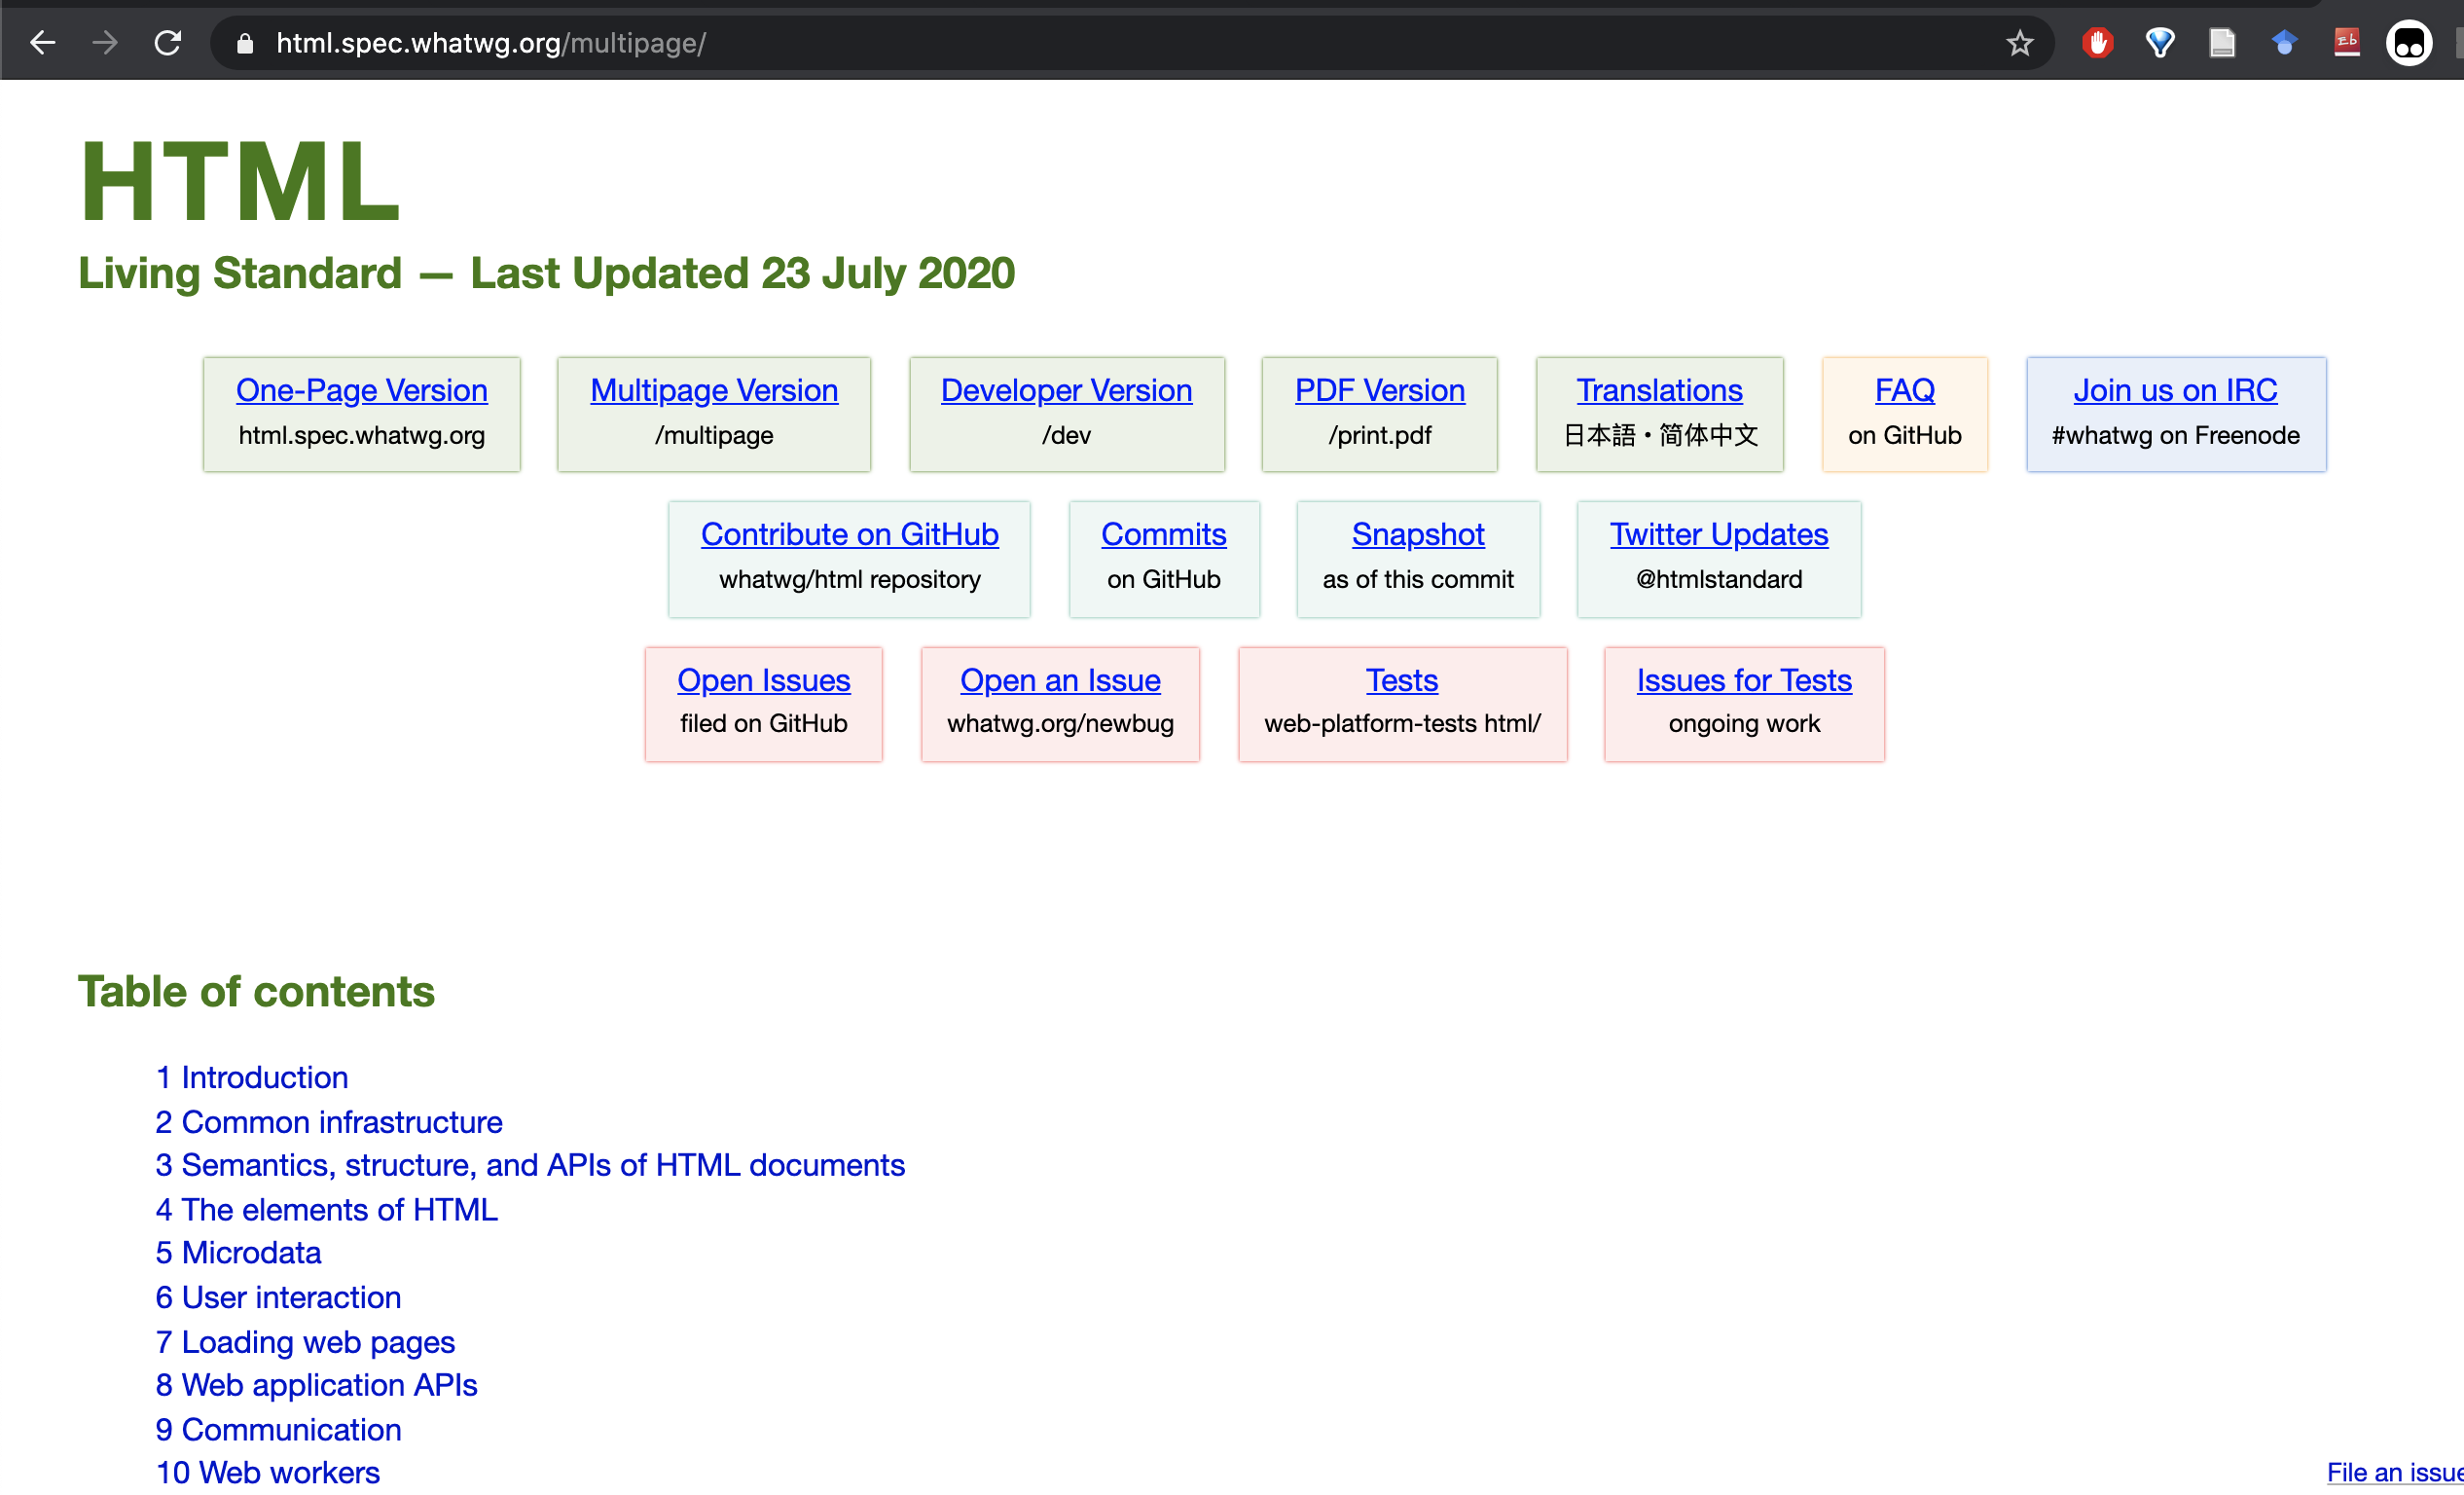
\includegraphics[trim=0cm 1cm 0cm 0cm, clip=true, width=0.75\textwidth]{img/html5standar}
\caption{HTML5 estandarra bizirik dago eta eguneraketak jasotzen jarraitzen du WHATWG webgunean: \href{https://html.spec.whatwg.org/multipage/}{https://html.spec.whatwg.org/multipage/}.}
\label{fig:quirksmode}
\end{figure}


\section{Historia apur bat}
\begin{alertinfo}{Hautazkoa}
Atal batzuk nahiko teknikoak bilaka daitezke. Hau bezalako ``Hautazko'' ohartxoak jarri ditugu horrelako azpiataletan, abisu gisa edo :)
\end{alertinfo}

HTML lengoaia hainbat bertsiotatik igaro da. Tim Berners Leek 1991n proposatu zuen HTMLren lehenengo zirriborroa, 18 etiketaz osatutakoa. Horietatik, 11 etiketa oraindik ere aurki daitezke HTML5en. Zirriborro horretan, \index{IETF} IETF (Internet Engineering Task Force) erakundeak 1993ko erdialdean HTML zehaztapenak argitaratu zituen. Ondoren, IETFk HTML espezifikazioa hobetzeko eta kudeatzeko 
``HTML Working Group'' izeneko taldea antolatu zuen. Talde horren lanaren lehenengo emaitza —beste enpresa eta erakunde batzuen ekarpena jaso ondoren, adibidez, Mosaic nabigatzaile aitzindariaren IMG etiketa— 1995ean plazaratu zen, HTML2 estandarra.

IETFk 1995ean HTML3ren proposamena jaso zuen, baina proposamena 6 hilabete geroago iraungi egin zen, inolako hobekuntzarik gabe. Bitartean, World Wide Web Consortium \index{W3C} (W3C) erakundea nabigatzaile propio bat garatzen hasia zen, \texttt{Arena} izenekoa, HTML3k proposatzen zituen berrikuntzak probatzeko asmoz (baita CSS estilo-orriak probatzeko ere). Garai hartan Netscape eta Internet Explorer sortu ziren, sekulako arrakastarekin. Nabigatzaileek eskatzen zituzten berrikuntzen kudeaketak eta HTMLk berak zuen ospeak IETFk zituen baliabideak gainezkatu zituzten. Hori dela eta, hurrengo urtetik hasita (1996), HTMLren espezifikazioa World Wide Web Consortium (W3C) erakundearen esku utzi zen.

W3C, IETFk egin zuen legez, kanpoko enpresen ekarpenak ere aztertu eta estandarra eguneratzen saiatu zen. Horren lehenengo fruitua 1997an izan zen, HTML4 estandarraren argitalpenarekin.

HTML 4.01 1999an argitaratu zen, nahiz eta akatsak zuzentzeko hainbat bertsio gehiago kaleratu behar izan zituzten 2001 arte.

2004an \index{WHATWG} WHATWG (\textit{Web Hypertext Application Technology Working Group}) lantaldea sortu zen, W3Ck HTMLren espezifikazioarekin zeraman erritmo motelari aurre egiteko. Baita W3C erakundeak HTML bertan behera utzi eta horren ordez XML lengoaian oinarritutako teknologiak sustatzeko hartutako erabakiari aurre egiteko ere.

WHATWG taldearen posta-zerrenda 2004ko ekainaren 4an sortu zen. Bertan Apple, Mozilla eta Opera nabigatzaileen ingeniariak HTML5 garatzen hasi ziren. WHATWGk Microsofteko ingeniari bati ere bertan parte hartzeko gonbita luzatu zion, baina ezezkoa jaso zuen.
 
2007an, WHATWGk bere HTML5en espezifikazioa W3Cren HTML garatzeko zuen lantaldeari eskaini zion, hortik abiatzeko haien lana. Izan ere, bertan adostu zuten HTML5 izena emango ziotela lantalde horien entregagaiari. Urte horretan bertan W3Ck eskaintza onartu zuen eta bi taldeen artean hainbat urtetan zehar lan egin ondoren, 2014ko urriaren 28an HTML5en lehenengo bertsio estandarra amaitu zuten.

% Zirriborro hau izan zen hain zuzen ere IETF (Internet Engineering Task Force) erakundeak 1993ko erdialdean erabili zuena HTML lengoaiaren lehenengo espezifikazioa argitaratzeko.

% \href{https://en.wikipedia.org/wiki/Mosaic_(web_browser)}{Mosaic (1993)}

% \href{https://en.wikipedia.org/wiki/Erwise}{Erwise (1992)}

% \href{https://en.wikipedia.org/wiki/ViolaWWW}{ViolaWWW (1992)}



\section{HTML5 etiketa berriak}

\subsection{HTML5 elementu berriak}

HTML5 bertsioak web dokumentuak eta aplikazioak sortzeko lengoaiaren bertsio zaharra hobetzen du, etiketa eta API (\textit{Application Programming Interfaces}) berriak eskainiz.

Zehazki, osagai grafiko berriak (\textit{<canvas>}, SVG —\textit{Scalable Vector Graphics}, grafiko bektorial-eskalagarriak—) eta multimedia (\textit{<audio>}, \textit{<video>}) eskaintzen ditu, \textit{plugin} edo API osagarririk erabili gabe.

Horretaz aparte, web dokumentuen edukiaren semantika hobetzeko elementuak gehitzen ditu: \textit{<section>}, \textit{<article>}, \textit{<header>} eta \textit{<nav>}, besteak beste.

HTML5en sorkuntzan hasiera-hasieratik dago errotuta gailu mugikorretarako web aplikazioak garatzeko lengoaia aproposa izan behar zuela, \textit{smartphone} eta \textit{tablet}-en ezaugarriak aprobetxatuz.

\subsection{Etiketa semantiko berriak}
Etiketa berriak edo HTML4 bertsioarekiko eguneratuak landuko ditugu hemen.

\index{DOCTYPE}\subsubsection{DOCTYPE hitzaurrea}
<!DOCTYPE html> hitzaurrearekin hasi behar dute HTML5en idatzitako web orriek. Horrekin, nabigatzaileak jakin ahalko du estandar berrienei jarraituz eraiki behar duela orria. DOCTYPE ingelesezko \textit{Document Type Declaration} (Dokumentu Motaren Erazagupena) hitzen akronimoa da.

Web orri baten HTML5 egitura zuzena dela egiaztatzeko online balidatzaileak erabil ditzakegu. Balidatzaile horiek egiten duten lehenengo gauza dokumentuaren sarrerari begiratzea da, jakin ahal izateko zer arauren kontra balioztatu behar duten uneko dokumentua. HTML5 lengoaian garatutako dokumentu zuzenek \textit{<!DOCTYPE html>} sarrerarekin hasi behar dute.

\vspace{0.5cm}
\begin{alertinfo}{Quirks mode}\index{Quirks mode}
    HTML5 diseinatzean ordura arte erabiltzen zen dokumentuen hitzaurrea erraztu nahi izan zen. Izan ere, nork gogoratzen du garai hartan erabiltzen zen hurrengo ``sarreratxoa''?
   \textit{<!DOCTYPE html PUBLIC \textquotedbl-//W3C/DTD HTML 4.01//EN\textquotedbl{}   \textquotedbl http://www.w3.org/TR/html4/strict.dtd\textquotedbl>}

Sarreratxo horri \texttt{DOCTYPE switch} deritzo. Agertuz gero, dokumentuak estandarrak betetzen dituela (estandarrei jarraituta idatzi dela) esan nahi du. Ez bada agertzen, estandarrei erdipurdi jarraituta edo estandarrak kontuan izan gabe idatzi dela esan nahi du (normalean webgune zaharretan gertatzen dena). Azken modu anarkiko horri \texttt{quirks mode} deritzo. HTML5en, DOCTYPE sarrera asko laburbildu da. Orain nahikoa da honela idaztea: \textit{<!DOCTYPE html>}
 
    \end{alertinfo}

\subsection{META etiketak}

META etiketak bilatzaileek erabiltzen dituzte batez ere jakin ahal izateko, automatikoki, zeintzuk diren dokumentuaren gako-hitzak (\textit{keywords}), hizkuntza, dokumentu mota edo erabilitako karaktere-jokoa. HTML5 sortu arte, hau zen maiz erabilitako META etiketa bat:
\begin{lstlisting}[numbers=none]
<meta http-equiv="content-type" content="text/html; charset=UTF-8">
\end{lstlisting}
Bertan, dokumentua HTMLz osatutako dokumentua zela zehazten zen. Baita UTF-8 karaktere-jokoa erabiltzen zela ere. Berriro, maiz erabilitako etiketa izateko, oso luzea, ezta? Orain, horrela laburbil daiteke, guztiz zuzena izanik:
\begin{lstlisting}[numbers=none]
<meta charset="utf-8">
\end{lstlisting}

Gauza bera gertatzen da estilo-orriak zehazteko garaian. Lehen honela idazten zena: 
\begin{lstlisting}[numbers=none]
<link type="text/css" rel="stylesheet" href="estiloak.css">
\end{lstlisting}
HTML5en beste era honetara idazten da:
\begin{lstlisting}[numbers=none]
<link rel="stylesheet" href="estiloak.css">
\end{lstlisting}
Edo JavaScript-en egindako \textit{skriptak} estekatzean lehen honela egiten zena: 
\begin{lstlisting}[numbers=none]
<script type="text/javascript" src="kodigoa.js"></script>
\end{lstlisting}
orain honela laburbildu da: 
\begin{lstlisting}[numbers=none]
<script src="kodigoa.js"></script>
\end{lstlisting}
Gauza bera orriaren hizkuntza adierazteko. Lehen:
\begin{lstlisting}[numbers=none]
<html xmlns="http://www.w3.org/1999/xhtml" lang="en" xml:lang="en"> 
\end{lstlisting}
orain:
\begin{lstlisting}[numbers=none]
<html lang="en">
\end{lstlisting}

Etiketa semantiko berriak \index{<header>}\index{<nav>}\index{<article>}\index{<section>}\index{<aside>}(\textit{<header>, <footer>, <nav>, <article>, <section>, <aside>}) hurrengo gaian jorratuko ditugu. Osagai grafiko berriak aztertzeko ere atal bereziak izango ditugu liburu honetan. Zehazki, \textit{<canvas>} eta <svg> etiketak 8. atalean zehazten dira eta multimediarekin lotutako etiketak, \textit{<audio>} eta \textit{<video>}, 9. atalean.

\section{Ariketak}

\begin{enumerate}

\item Bihurtu HTML5 formatura HTML4n programatutako lerro hauek:

\begin{lstlisting}[numbers=none]
<meta http-equiv="content-type"content="text/html; charset=UTF-8">
\end{lstlisting}
     
\begin{lstlisting}[numbers=none]
<link type="text/css" rel="stylesheet" href="estiloak.css">
\end{lstlisting}
    
\begin{lstlisting}[numbers=none]
<script type="text/javascript" src="kodigoa.js"></script>
\end{lstlisting}

\begin{lstlisting}[numbers=none]
<html xmlns="http://www.w3.org/1999/xhtml" lang="eu_ES" xml:lang="eu_ES">
\end{lstlisting}

\item Bihurtu HTML5 formatura HTML4n programatutako adibide hau:

\begin{lstlisting}[language=HTML,numbers=none]
<!DOCTYPE html PUBLIC "-//W3C//DTD XHTML 1.0 Strict//EN"
"http://www.w3.org/TR/xhtml1/DTD/xhtml1-strict.dtd">
<html xmlns="http://www.w3.org/1999/xhtml"
 lang="eu_ES"
 xml:lang="eu_ES">
 <head>
 <meta charset="utf-8" />
 <title>1. Ariketa </title>
 <link href="css/style.css" rel="stylesheet" />
 </head>
 <body>
 </body>
</html>
\end{lstlisting}
\end{enumerate}
%% 2. HTML5 Egitura osagaiak
\chapter{HTML5 egitura-osagaiak}

Hainbat etiketa semantiko berri aurki ditzakegu HTML5en  \href{https://html.spec.whatwg.org/multipage/sections.html}{espezifikazioan}\footnote{https://html.spec.whatwg.org/multipage/sections.html}. Horietatik, garrantzitsuenak eta askotan erabiltzen direnak, \textit{header}, \textit{footer}, \textit{nav}, \mbox{\textit{article}}, \textit{section} eta \textit{aside} dira.

\index{header}
Deskribapen eta eztabaida sakon eta aspergarri bat eman ordez, hobe iruditu zait adibideekin aztertzea. Dena den, etiketa garrantzitsu horien deskribapen oso labur batekin hasiko gara.
% <header>  <footer> <nav> <article> <section> <aside> 


\textbf{<header>} Webgunearen goiburua irudikatzeko etiketa. 

\index{footer}
\textbf{<footer>} Webgunearen orri-oina irudikatzeko etiketa. Adi, ez da beti orriaren beheko aldean zertan agertu. 

\index{nav}
\textbf{<nav>} Webgunetik nabigatzeko menua (edo antzeko funtzionalitatea) gordeko du.

\index{article}
\textbf{<article>} Bere baitan zentzua daukan eduki puska gordeko du. Etiketa honen barruan gordetzen dugun edukiak zentzua izan beharko luke RSS jario baten elementu gisa (adibidez, egunkari baten berriak emateko RSS baten barruan, berri-laburpen bat <article> bat izan daiteke)

\index{section}
\textbf{<section>} Artikuluak (<article> osagaiak) gaiaren arabera multzokatzeko erabil daitezke, baina baita artikulu baten barruan dagozkion atalak zehazteko ere.

\index{aside}
\textbf{<aside>} Alboko edukiak eduki bloke bat zehazten du, bere inguruan dagoen eduki nagusiarekin zerikusia duen zerbait gordetzeko (baina eduki nagusiaren jarioarekin guztiz bat ez datorren zerbait).

\begin{figure}[ht]
	\centering
\begin{tikzpicture}
\node[anchor=south west,inner sep=0] (image) at (0,0)
   {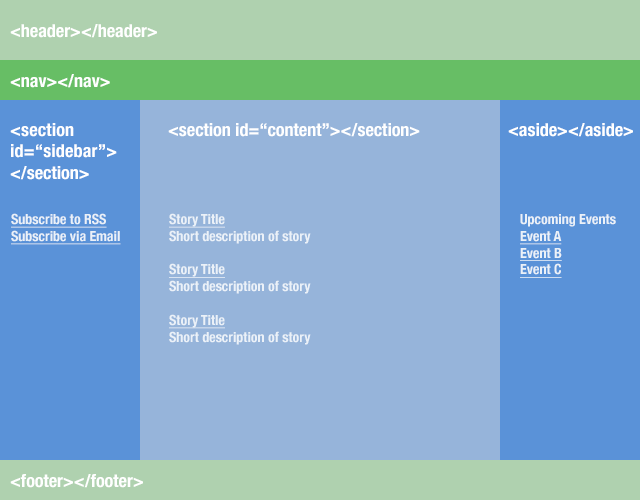
\includegraphics[trim=0cm 0cm 0cm 0cm, clip=true, width=0.75\textwidth]{img/structural_content}};
%    \begin{scope}[x={(image.south east)},y={(image.north west)}]
% \fill[color=red] (0.503, 0.44) rectangle(0.533, 0.685);
%\end{scope}
\end{tikzpicture}
\caption{HTML5 egitura-osagaiak. Iturria: \href{http://stackoverflow.com/a/24765186/243532}{http://stackoverflow.com/a/ 24765186/243532}.}
\label{fig:html5etiketasematikoak}
\end{figure}

Goazen adibideetara. Lehenengoa, nola ez, \href{http://stackoverflow.com/a/24765186/243532}{StackOverflow webgunetik}\footnote{http://stackoverflow.com/a/24765186/243532} hartua da eta \ref{fig:html5etiketasematikoak}. irudian ikus dezakegu. Bertan orri baten goiburua adierazteko \textit{header} etiketa erabiltzen dela adierazten dugu. Ildo beretik, askotan nabigatzeko barra bat ikusten da, \textit{nav} etiketekin adierazita irudian. Orri baten atal nagusiak, edukia bera eta dokumentuaren azpiataletik nabigatzeko esteka zuzenak, \textit{section} etiketen barruan sartuko ditugu. Uneko dokumentuarekin lotura zuzena ez baina zeharkako lotura duen beste eduki bat kodean antolatzeko, \textit{aside} etiketa erabil dezakegu. Bukatzeko, orri-oinak \textit{footer} gisa markatuko ditugu. Aipatutakoa, antolaketa modu bat da, W3Ck gomendatzen duena hain zuzen ere, baina kontuz, zenbait xehetasun daude. Alde batetik, \textit{footer} etiketaren edukiak ez du beti dokumentuaren beheko aldean agertu behar, baliteke beste oin batzuk izatea. \textit{Section} baten barruan artikulu (\textit{article}) batzuk izan ditzakegu... eta alderantziz! Ikus ditzagun adibide zehatz batzuk hau guztia ondo barneratzeko.

\begin{figure}[ht]
	\centering
\begin{tikzpicture}
\node[anchor=south west,inner sep=0] (image) at (0,0)
   {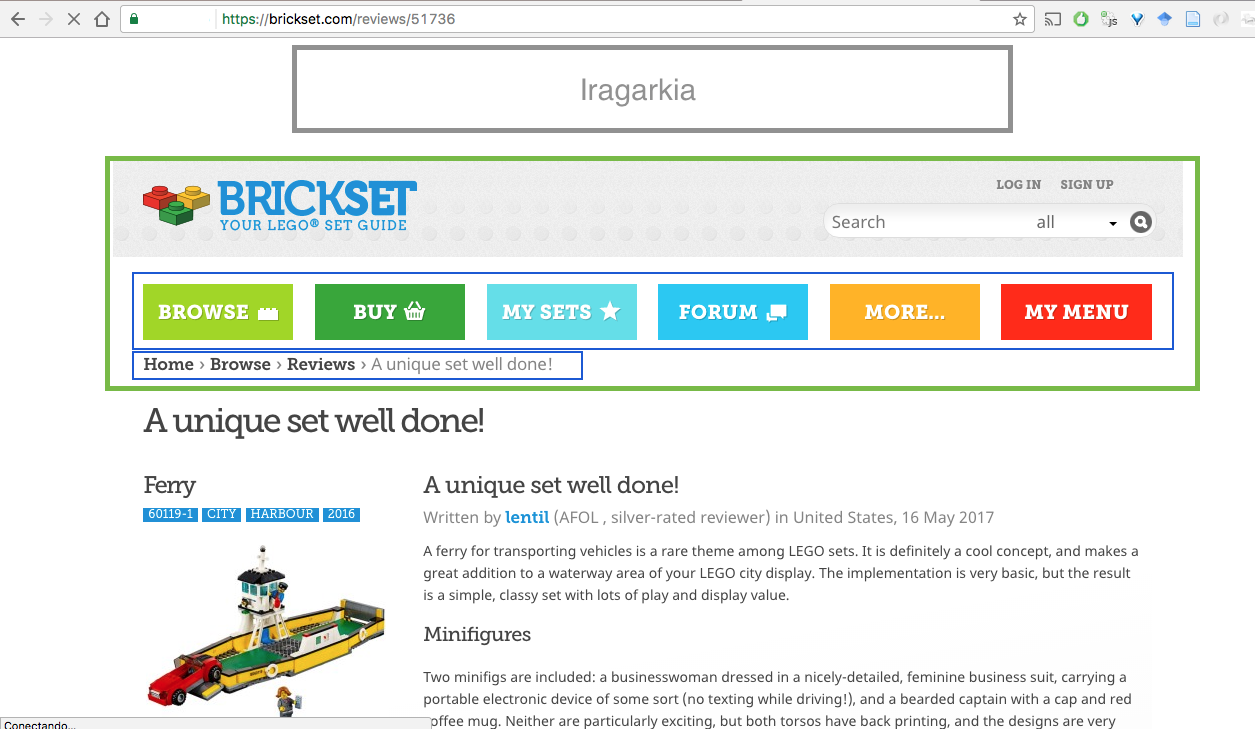
\includegraphics[trim=0cm 0cm 0cm 0cm, clip=true, width=.75\textwidth]{img/lego_html}};
\end{tikzpicture}
\caption{HTML5 egitura-osagaiak.}
\label{fig:legohtml5etiketak}
\end{figure}

\begin{figure}[ht]
	\centering
\begin{tikzpicture}
\node[anchor=south west,inner sep=0] (image) at (0,0)
   {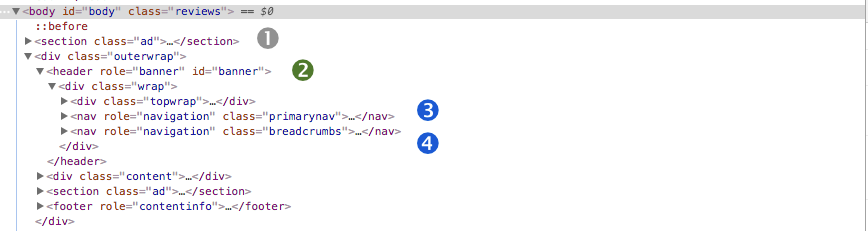
\includegraphics[trim=0cm 0cm 0cm 0cm, clip=true, width=\textwidth]{img/html_kodea}};
\end{tikzpicture}
\caption{HTML5 etiketa semantikoak: Lego orriaren adibidea. Kodea.}
\label{fig:legohtml5etiketakkodea}
\end{figure}


Adibidez, har dezagun  \href{https://brickset.com/reviews/51736}{Lego webgunearen orri bat}\footnote{https://brickset.com/reviews/51736},  \ref{fig:legohtml5etiketak}. irudian ikus dezakeguna. Orriari dagokion HTML kodea  \ref{fig:legohtmledukiakodea} irudian daukagu. Bertan 1. puntuan (grisez), \textit{section} bat aurkitzen dugu, orriaren iragarkia edo \textit{banner-a} adierazteko. Jarraian, 2. puntuan, \textit{header} etiketa, Lego webgunetik nabigatu ahal izateko botoiak, bilatzailea eta ogi-papurren bidea adierazteko. Goiburuaren (\textit{header-}en) barruan, bi \textit{nav} etiketa, nabigatzeko lehenengo botoi-barra eta ogi-papurren bidea markatzeko.

\begin{figure}[ht]
	\centering
\begin{tikzpicture}
\node[anchor=south west,inner sep=0] (image) at (0,0)
   {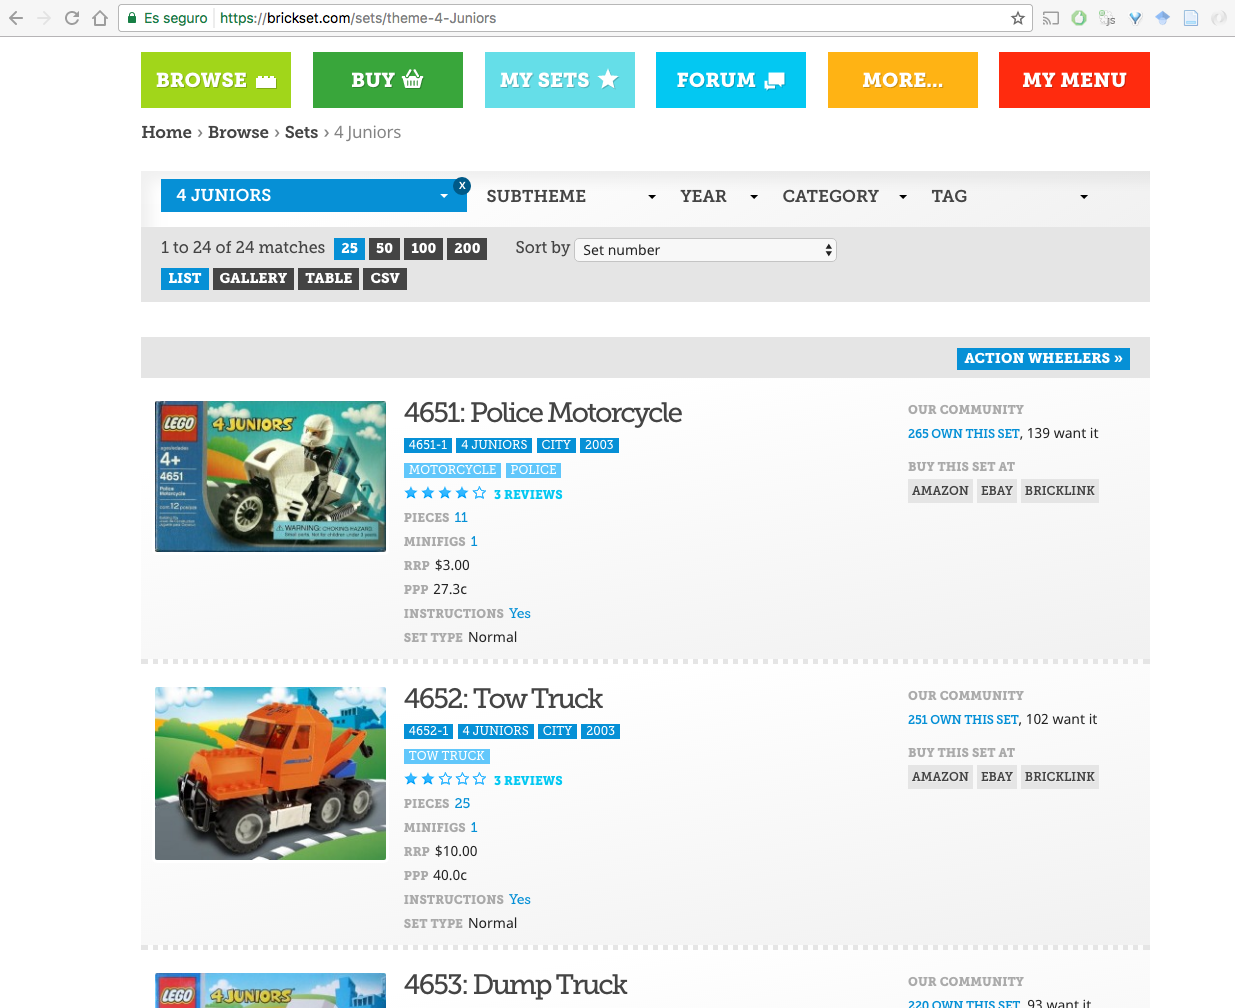
\includegraphics[trim=0cm 0cm 0cm 0cm, clip=true, width=.75\textwidth]{img/lego_content}};
\end{tikzpicture}
\caption{HTML5 egitura-osagaiak. Eduki nagusia.}
\label{fig:legohtml5edukia}
\end{figure}

\begin{figure}[ht]
	\centering
\begin{tikzpicture}
\node[anchor=south west,inner sep=0] (image) at (0,0)
   {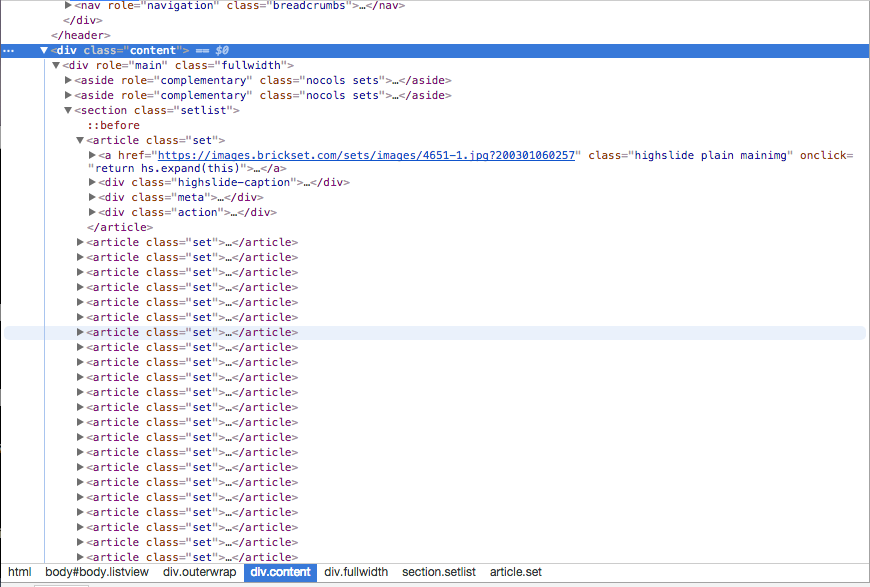
\includegraphics[trim=0cm 0cm 0cm 0cm, clip=true, width=0.75\textwidth]{img/lego_content_kodea}};
\end{tikzpicture}
\caption{HTML5 etiketa semantikoak: Lego orriaren adibidea (II). Kodea.}
\label{fig:legohtmledukiakodea}
\end{figure}

Lego bilduma-bilatzailean sartuz gero, goiburua (\textit{header}) berdina bada ere, edukia noski, aldatzen da (ikus \ref{fig:legohtml5edukia}. irudia). Eduki horri dagokion kodea \ref{fig:legohtmledukiakodea}. irudian aztertuko dugu. Bertan, bi \textit{aside} daude, figura-bildumetatik nabigatzeko eta iragazketa egiteko inprimakiekin. Jarraian, \textit{section} etiketaren barruan, figura-bilduma guztiak, banan-banan, bakoitza \textit{article} etiketa baten barruan.

\section{Ariketak}

\begin{enumerate}

\item Ordezkatu <div> etiketa bakoitza dagokion HTML5 etiketa semantiko egokiaz:
 
 \begin{lstlisting}[language=HTML,numbers=none]
 <div id="header">
<h1> Goi mailako goiburu bat naiz</h1
</div>
<div id="footer">
 <h3> UPV/EHU </h3>
 <p> 2020/21 ikasturtea </p>
</div>
 \end{lstlisting}
 
 
\item Ordezkatu <div> etiketa bakoitza dagokion HTML5 etiketa semantiko egokiaz:

 \begin{lstlisting}[language=HTML,numbers=none]
 <div id="navigation">
<ul>
<li>Euskal Herrian</li>
<li>Datuak munduan</li>
<li>Shock ekonomikoa</li>
<li>Buletin berezia</li>
</ul>
</div>
  \end{lstlisting}
 
 \item Ordezkatu <div> etiketa bakoitza dagokion HTML5 etiketa semantiko egokiaz eta bihurtu goiburu-etiketak h1 eta h2:

\begin{lstlisting}[language=HTML,numbers=none]
<div class="section">
 <h2>Berrinfekzio kasuen berri eman dute Belgikan eta
Herbehereetan ere</h2>
 <h3>OME Osasunaren Mundu Erakundearen iritzia</h3>
 <p>Astelehenean jakin zen COVID-19 birusarekin berrinfektutako
pertsona bat atzeman zutela lehen aldiz...</p>
</div>
 \end{lstlisting}
 
 \item Gehitu beharrezko <article> etiketak:
 \begin{lstlisting}[language=HTML,numbers=none]
 <section id="koronabirusa">
<header>
 <h1>Eguneraketa</h1>
</header>
 <h2>Osasun sistemaren gaitasuna</h2>
 <p>Urkulluren ustez, osasun sistemaren gaitasuna ''bermaturik''
dago</p>
 <h2>Berrinfekzioak</h2>
 <p>Berrinfekzio kasuen berri eman dute Belgikan eta Herbehereetan
ere</p>
</section>
\end{lstlisting}

\item Ordezkatu <p class=\textquotedbl{}aside\textquotedbl{}> etiketa dagokion HTML5eko osagai egokiaz:

\begin{lstlisting}[language=HTML,numbers=none]
<section id="koronabirusa">
<header>
 <h1>Eguneraketa</h1>
</header>
<article>
 <h2>Osasun sistemaren gaitasuna</h2>
 <p>Urkulluren ustez, osasun sistemaren gaitasuna 
 ''bermaturik''
dago</p>
 <p class="aside">Pedro Sanchez Espainiako Gobernuko presidenteak ere agerraldia egin zuen atzo...</p>
</article>
</section>

\end{lstlisting}

\item 

Bihurtu HTML5 formatura HTML4n programatutako
adibide hau:

\begin{lstlisting}[language=HTML,numbers=none]

<!DOCTYPE html PUBLIC "-//W3C//DTD XHTML 1.0 Strict//EN"
"http://www.w3.org/TR/xhtml1/DTD/xhtml1-strict.dtd">
<html xmlns="http://www.w3.org/1999/xhtml"
 lang="eu_ES"
 xml:lang="eu_ES">
 <head>
 <meta charset="utf-8" />
 <title>1. Ariketa</title>
 <link href="css/style.css" rel="stylesheet" />
 </head>
 <body>
<div id="header">
<h1> Koronabirusa</h1
<h2>Euskal Herrian eta Munduan</h2>
</div>
<div id="navigation">
 <ul>
 <li>Euskal Herrian</li>
 <li>Datuak munduan</li>
 <li>Shock ekonomikoa</li>
 <li>Buletin berezia</li>
 </ul>
</div>
<div id="section">
 <h2>Zelaa aztertzen ari da COVID-19a duten haurren gurasoei
gaixo agiria ematea</h2>
<div class="article">
 <h3>Bihar elkartuko dira autonomia erkidegoetako
ordezkariekin</h3>
 <p>Maskarak, gel hidroalkoholikoak, PCRak, distantzia...
Funtsean, COVID-19ak baldintzatuko du 2020-2021eko ikasturtea.</
p>
 <p class="aside">Bihar bilera: Zelaak azaldu duenez, bihar
elkartuko dira autonomia erkidegoetako ordezkariekin</p>
</div>
<div class="article">
 <h3>Berrinfekzio kasuen berri eman dute Belgikan eta
Herbehereetan ere</h3>
 <p>
 OME Osasunaren Mundu Erakundeak esan du berrinfekzioen
gaineko berriak oraindik ''anekdotikoak'' direla, eta zer ikertua
franko dagoela
 </p>
</div>
</div>
<div id="footer">
 <h3> UPV/EHU </h3>
 <p> 2020/21 ikasturtea </p>
</div>
</body>
</html>
\end{lstlisting}

\item Bihurtu HTML5 formatura HTML4n programatutako
adibide hau:

\begin{lstlisting}[language=HTML,numbers=none]

<!DOCTYPE html PUBLIC "-//W3C//DTD HTML 4.01//EN"
"http://www.w3.org/TR/html4/strict.dtd">
<html>
<head>
<meta http-equiv="content-type" content="text/html; charset=UTF-8">
<title>Taberna</title>
<link type="text/css" rel="stylesheet" href="taberna.css">
<script type="text/javascript" src="taberna.js"></script>
</head>
<body>
<h1>Ongi Etorri Tabernara</h1>
<p>
<img src="edariak.gif" alt="Edariak">
</p>
<p>
Arratsaldero elkartzen gara xake edo mus partida batzuk jolastera <a
href="garagoardoak.html">garagardo batzuk</a> edaten dugun bitartean,
solasaldi ederraz gozatuz. WiFi sarea ere badugu, konexio on batekin.
</p>
</body>
</html>
\end{lstlisting}
\end{enumerate}

%% 3. JS 5 minututan
\chapter{JavaScript bost minututan}

HTML5en arrakasta ez dago sartu dituen HTML etiketa semantiko berrietan oinarrituta, \index{API} JavaScript API berrietan baizik. API horietan murgildu baino lehenago, ezinbestekoa dugu gure JavaScript-en ezagupen herdoilduak apur bat berritu eta garbitzea. Horretarako, atal honetan, JavaScript lengoaiak eskaintzen dituen funtzionalitate nagusiak izango ditugu hizpide. Berriro, jada JavaScript apur bat badakizula onartuko dugu eta soilik HTML5eko APIak ondo erabili ahal izateko  funtzionalitate garrantzitsuenetan sakonduko dugu.


\section{Aldagaien erazagupena}
\index{var}\index{let}\index{const} Nola deklaratu aldagai bat JavaScript-en? Zer erabili, \textit{var}, \textit{let} edo \textit{const}? Galdera hauei erantzuten saiatuko gara, labur-labur.

Orain dela urte batzuk (\textit{let} eta \textit{const} existitzen ez zirenean ere), honela erazagutu behar ziren aldagaiak:

%\begin{minipage}{\linewidth}
\begin{lstlisting}[language=JavaScript]
// Iruzkina
var zabalera ; // hasieratu gabeko aldagai baten erazagupena
var txapeldunak = 2;
var txapeldunak = 4; /* ez da batere gomendagarria aldagai bat ber-erazagutzea, baina 'var' erabiliz, posible da */
var irakitePuntua = 100;
var irakitePuntua = "Ehun"; /* aldagai mota dinamikoki alda daiteke. Berriro, ez da batere gomendagarria, baina egin daiteke */
var nahikoAdin = false;
var temp = 100, lema = "Kaixo";
temp = (temp - 12) * 5 / 9;   // Adierazpen matematikoa
lema = lema + " mundua!"; 
var pos = Math.random(); 

\end{lstlisting}
%\end{minipage}

Arau nagusiak hiru dira:
\begin{itemize}
\item Aldagaiaren izena hizki batez (edo \_ edo \$ karaktereez) hasten da.
\item Jarraian, zenbakiak edo hizkiak edo \_ edo \$ karaktereak kateatu daitezke, hainbat aldiz.

\item Hitz erreserbatuak daude (gako-hitzak), erabili ezin direnak:

\fbox{\begin{minipage}{\linewidth}
abstract, as, boolean, break, byte, case, catch, char, class,
continue, const, debugger, default, delete, do, double, else, enum,
export, extends, false, final, finally, float, for, function, goto,
if, implements, import, in, instanceof, int, interface, is, long,
namespace, native, new, null, package, private, protected, public,
return, short, static, super, switch, synchronized, this, throw,
throws, transient, true, try, typeof, use, var, void, volatile, 
while, with
\end{minipage}}
\end{itemize} 

Gaur egun, \textit{\hlc[lightgray]{var}} ez erabiltzea gomendatzen da. Horren ordez \textit{\hlc[lightgray]{let}} (aldagaiak deklaratzeko) eta \textit{\hlc[lightgray]{const}} (konstanteak erazagutzeko) lehenesten dira. \textit{\hlc[lightgray]{Let}} aldagai bat ezin da birritan erazagutu (saiatuz gero, errore bat jasoko dugu), baina haren balioa, ordea, bai, alda daiteke. \textit{\hlc[lightgray]{Const}} baten kasuan, berriz, ezin da ez berrerazagutu, ezta haren balioa aldatu ere. 

\begin{minipage}{\linewidth}
\begin{lstlisting}[language=JavaScript]
// Let
let zabalera ; // hasieratu gabeko aldagai baten erazagupena
let txapeldunak = 2;
let txapeldunak = 4; // ERRORE bat jasoko dugu
const PI = 3.14;
PI = 3.1415; // ERRORE BAT jasoko dugu, jada konstantea zehaztuta baitago

\end{lstlisting}
\end{minipage}



\section{\textit{While} eta \textit{for} begiztak}

Iterazioak lortzeko (datu-egiturak zeharkatzeko edo baldintza bat betetzen den bitartean kode zati bat exekutatzeko), \textit{while} eta \textit{for} begiztak erabiltzen dira. Noizbait beste programazio-lengoaia batean programatu baduzu, ez duzu inolako arazorik izango kode bloke hauek ulertzeko:

\begin{minipage}{\linewidth}
\begin{lstlisting}[language=JavaScript]
var i=0;
while (i < kafeKop) {
 kafeaEdan();
 i = i + 1;
}

for (var i=0; i < kafeKop; i++){
 kafeKop();
}
\end{lstlisting}
\end{minipage}

\section{Baldintzazko adierazpenak}
\textit{if-then-else} baldintzazko adierazpen klasikoa ere beste lengoaia batzuetan bezala erabiltzen da, honako patroiari jarraituz:

\begin{verbatim}
if (baldintza) {
   baldintza betetzen denenean exekutatu beharreko kodea
} else {
   baldintza betetzen EZ denean exekutatu beharreko kodea
}
\end{verbatim}

Adibidez:

%\begin{minipage}{\linewidth}
\begin{lstlisting}[language=JavaScript]
if (nahikoAdin) {
 emaitza = "Gidatu ahal duzu!";
} else {
 emaitza = "Tamalez, oraindik ezin duzu gidatu.";
}
\end{lstlisting}
%\end{minipage}

\section{Arrayak}
\index{Array}
Arrrayak datu multzo bat memorian gordetzeko datu-egiturak dira. Adibidez, bost zenbaki gorde nahi baditugu taula izeneko array batean:

%\begin{minipage}{\linewidth}
\begin{lstlisting}[language=JavaScript]
let taula = new Array();
taula[0] = 5.1;
taula[1] = 6.1;
taula[2] = -2.5;
taula[3] = -3;
taula[4] = -4;
\end{lstlisting}
%\end{minipage}
 

Edo modu laburrean idatzita (aurrekoaren baliokidea):
 
\begin{minipage}{\linewidth}
\begin{lstlisting}[language=JavaScript]
let taula = [5.1, 6.1, -2.5, -3 -4];
\end{lstlisting}
\end{minipage}

 Beste lengoaia batzuetan array baten tamaina finkoa da bai eta gordetzen dituen datu motak ere. JavaScript-en ez da horrela, alegia, array baten tamaina ez da hasiera-hasieratik zehaztu behar (dinamikoa da) eta barruan gordetzen diren balioen datu motak ere ez du zertan berdina izan.
 
\begin{minipage}{\linewidth}
\begin{lstlisting}[language=JavaScript]
// JavaScript-en arrayak dinamikoak dira.
// Demagun taula aldagaia erazagutu eta hasieratu dugula

let taula = [];
// Jarraian, hau eginez gero:

taula[5] = 38; 

// Orain taulan 6 posizio izango ditugu eta 6.ean (0-tik
// hasten dira indizeak) 38 zenbakia aurkituko dugu. 
// Tartean, "undefined" elementuak.
// Beraz, orain taularen luzera eskatuz gero, 6 emango digu

console.log(taula.length); // Emaitza: 6

// zenbakiak gorde baditugu ere, hurrengo posizioan string bat gorde dezakegu, arazorik gabe (eta honekin, berriro, dinamikoki luzatu dugu arrayaren tamaina)

taula[6] = "Sagarra";

console.log(taula); // Emaitza: (7) [empty x 5, 38, "Sagarra"]

\end{lstlisting}
\end{minipage}
 
% Ikusi dugun bezala, array batek hainbat balio ezberdin aldagai baten barruan gorde ditzake. Balio horiek  indize baten bidez atzitu daitezke:
% 
% \begin{minipage}{\linewidth}
% \begin{lstlisting}[language=JavaScript]
% let markak = new Array();
% markak[0]="Saab";
% markak[1]="Volvo";
% markak[2]="BMW";
% \end{lstlisting}
% \end{minipage}
% 
% Badago beste modu laburragoa arrayak zehazteko:
% 
% \begin{lstlisting}[language=JavaScript]
% let markak = new Array("Saab","Volvo", "BMW");
% \end{lstlisting}
% 
% edo literalak erabiliz:
% \begin{lstlisting}[language=JavaScript]
% let markak = ["Saab","Volvo", "BMW"];
% \end{lstlisting}
% 
% JavaScript-en array baten barruan gordetzen diren elementuak ez dute zertan datu-mota berdina izan behar:
% 
% \begin{minipage}{\linewidth}
% \begin{lstlisting}
% let nireArray = new Array();
% nireArray[0] = Math.random(); // float
% nireArray[1] = "kate bat"; // string
% nireArray[2] = markak; // array
% \end{lstlisting}
% \end{minipage}
% 

\index{Array}
Jarraian, \hl{Array} klaseak eskaintzen dituen beste metodo interesgarri batzuk aztertuko ditugu:

\fbox{\begin{minipage}{\linewidth}
concat, indexOf, join, lastIndexOf, pop, push, reverse,
shift, slice, sort, splice, toString, unshift, valueOf
while, with
\end{minipage}}

% Length (array-aren luzera) da askotan erabiliko dugun atributu bat. Esaterako, aurreko adibidean:

%\begin{verbatim}
% nireArray.length // 3 itzuliko du.    
%\end{verbatim}
\vspace{5mm} %5mm vertical space
\index{concat()} Elementuak kateatzeko (\textit{concat}):

\begin{minipage}{\linewidth}
\begin{lstlisting}[language=JavaScript]

let batzuk = ["Carlos", "Lierni"];
let besteak = ["Eneritz", "Tadeo", "Linus"];
let denak = batzuk.concat(besteak);
// denak: ["Carlos", "Lierni", "Eneritz", "Tadeo", "Linus"]
\end{lstlisting}
\end{minipage}

\index{indexOf()} Elementu baten indizea lortzeko (\textit{indexOf}):

\begin{minipage}{\linewidth}
\begin{lstlisting}[language=JavaScript]
let taldeak = ["Athletic", "Barcelona", "Erreala"];
let ind = taldeak.indexOf("Erreala"); // ind = 2
\end{lstlisting}
\end{minipage}

\index{join()} Elementuak lotzeko (\textit{join}):

\begin{minipage}{\linewidth}
\begin{lstlisting}[language=JavaScript]
let frutak = ["Banana", "Laranja", "Sagarra", "Mango"];
let energia = frutak.join(".");
// energia = "Banana.Laranja.Sagarra.Mango"
\end{lstlisting}
\end{minipage}

\index{lastIndexOf()} Elementu batek arrayan duen azken posizioaren indizea lortzeko (\textit{lastIndexOf}):

\begin{minipage}{\linewidth}
\begin{lstlisting}[language=JavaScript]
let lengoaiak = ["Pascal", "Ada", "C++", "Java", "JavaScript", "Ada"];
lengoaiak.lastIndexOf("Ada"); // 5
\end{lstlisting}
\end{minipage}

\index{pop()} Arrayaren azken elementua lortzeko eta arraytik ateratzeko (\textit{pop}):

\begin{minipage}{\linewidth}
\begin{lstlisting}[language=JavaScript]
let paloak = ["urreak", "kopak", "ezpatak", "bastoiak"];
paloak.pop(); // "bastoiak"
// paloak: ["urreak", "kopak", "ezpatak"]
\end{lstlisting}
\end{minipage}

\index{shift()} Arrayaren lehen elementua arraytik atera (\textit{shift}):

\begin{minipage}{\linewidth}
\begin{lstlisting}[language=JavaScript]
let paloak = ["urreak", "kopak", "ezpatak", "bastoiak"];
paloak.shift(); // "urreak"
// paloak: ["kopak", "ezpatak", "bastoiak"]
\end{lstlisting}
\end{minipage}


\index{push()} Arrayaren azken elementua txertatzeko (\textit{push}):

\begin{minipage}{\linewidth}
\begin{lstlisting}[language=JavaScript]
// push metodoak elementua azken posizioan txertatu eta hori egin ondoren arrayan zenbat elementu dauden bueltatzen du
let paloak = ["urreak", "kopak", "ezpatak"];
paloak.push("bastoiak"); // 4
// paloak: ["urreak", "kopak", "ezpatak", "bastoiak"]
\end{lstlisting}
\end{minipage}

\index{reverse()}  Arrayaren elementuak iraultzeko (\textit{reverse}):

\begin{minipage}{\linewidth}
\begin{lstlisting}[language=JavaScript]
let paloak = ["urreak", "kopak", "ezpatak", "bastoiak"];
paloak.reverse();
// paloak : ["bastoiak", "ezpatak", "kopak", "urreak"]
 
\end{lstlisting}
\end{minipage}


Dimentsio anitzeko arrayak ere sor daitezke (alegia, arrayez osatutako arrayak):

\begin{minipage}{\linewidth}
\begin{lstlisting}[language=JavaScript]

let elementuak = [[1,2],[3,4],[5,6]];
console.log(elementuak[0][0]); // 1 ematen du
\end{lstlisting}
\end{minipage}

10 x 20 elementuz osatutako array bat sortzeko adibidearekin bukatuko dugu:

\begin{minipage}{\linewidth}
\begin{lstlisting}[language=JavaScript]

let x = new Array(10);
 for (let i = 0; i < 10; i++) {
 x[i] = new Array(20);
 }
 
 x[5][12] = 3.0;  // elementu bat txertatu (5,12) gelaxkan
\end{lstlisting}
\end{minipage}
 
 \section{Ariketak}


 Irakurri \hlc[lightgray]{var}, \hlc[lightgray]{let} eta \hlc[lightgray]{const} klausulen arteko ezberdintasunak lantzen dituen dokumentu hau: \\
 \href{ https://dev.to/sarah\_chima/var-let-and-const--whats-the-difference-69e}{https://dev.to/sarah\_chima/var-let-and-const--whats-the-difference-69e}.
    
    \textbf{Adi}! Garatzaileei laguntzeko eta JavaScript-en modu azkarrean gauzak probatu ahal izateko Google Chrome-k bere Chrome DevTools kontsolan \textit{let} aldagaiak behin baino gehiagotan erazagutzen uzten du. Firefox-en lan egiten baduzu, ez da hori gertatuko. Ikus: \href{https://umaar.com/dev-tips/214-redeclare-let-console/}{https://umaar.com/dev-tips/214-redeclare-let-console/}.
    
\begin{enumerate}
    \item Zer lortuko dugu pantailan honakoa idaztean?    
\begin{lstlisting}[language=JavaScript,numbers=none]
var tester = "hey hi";
function newFunction() {
   var hello = "hello";
}
console.log(hello);

\end{lstlisting}

\item Posible al da hau egitea?
\begin{lstlisting}[language=JavaScript,numbers=none]
var greeter = "hey hi";
var greeter = "say Hello instead";   
    \end{lstlisting}

\item  Posible al da hau egitea errorerik jaso gabe? Baiezkoan, nola deitzen zaio JavaScript-eko
ezaugarri honi (aldagai baten balioa kodean deklaratu baino lehenago erabiltzeari)?
\begin{lstlisting}[language=JavaScript,numbers=none]
console.log (greeter);
var greeter = "say hello"    
    \end{lstlisting}

\item  Zer bistaratuko da kontsolan kode hau exekutatzean?
\begin{lstlisting}[language=JavaScript,numbers=none]
var ind = 0;
for(var ind=3; ind<10; ind++); // gorputzik gabeko begizta
console.log(ind);

\end{lstlisting}

\item Zer inprimatzen da kode honen amaieran?
(adi, DevTools erabiltzen ari bazara, gogoratu fitxa berri bat irekitzeaz testuinguru berri batetik
abiatzeko beti)

\begin{lstlisting}[language=JavaScript,numbers=none]
let ind = 0;
for(let ind=3; ind<10; ind++); // gorputzik gabeko begizta
console.log(ind);
\end{lstlisting}

\item Honakoa egin daiteke errorerik jaso gabe?

\begin{lstlisting}[language=JavaScript,numbers=none]
let agurra = "Hola";
let agurra = "Kaixo"
 \end{lstlisting}
 
 \item  Eta hau?
\begin{lstlisting}[language=JavaScript,numbers=none]
var agurra = "Hola";
var agurra = "Kaixo";
 \end{lstlisting}
 
 \item  Honakoa egin daiteke errorerik jaso gabe?
 
\begin{lstlisting}[language=JavaScript,numbers=none]
console.log (greeter);
let greeter = "say hello";
 \end{lstlisting}
 (Adi, ez da 3. ariketaren berdina)
 
 \item Badago errorerik hemen? Zer lortzen dugu pantailan?
\begin{lstlisting}[language=JavaScript,numbers=none]
const AGUR="agur!"
AGUR="adiós!";
 \end{lstlisting}
 
 \item Badago errorerik hemen? Zer lortzen dugu pantailan?
\begin{lstlisting}[language=JavaScript,numbers=none]
const AGUR="agur!";
if (true){
 const AGUR="adiós!";
}
console.log(AGUR);
 \end{lstlisting}
 
 \item  Badago errorerik hemen? Zer lortzen dugu pantailan?
 
\begin{lstlisting}[language=JavaScript,numbers=none]
const hiztegia = {
 hola : "kaixo",
 casa : "etxea"
};
hiztegia.hola = "iepa!";
console.log(hiztegia.hola);
 \end{lstlisting}

\end{enumerate}

Bigarren ariketa multzoan arrayak erabiliko ditugu. Lasai hartu, arrayek JavaScripten badute bere zailtasuna eta.
 
 \begin{enumerate}
     \item Demagun 3 puntuz osatutako arraya sortu dugula:
     \begin{lstlisting}[language=JavaScript]
     
function Point(x,y){
 this.x = x;
 this.y = y;
}
let puntuak = [new Point(5,0), new Point(11,1), new Point(2,2)]

\end{lstlisting}

Programa ezazu array horren barruan dauden eta x koordenatua > 10 balioa duten
puntuak ezabatzeko \textit{script}a. Proba ezazu zure soluzioa array hauekin ere:

\begin{lstlisting}[language=JavaScript]
let puntuak = [new Point(5,0), new Point(11,1), new Point(15,1), new Point(2,2)];
let puntuak = [new Point(5,0), new Point(4,1), new Point(5,2), new Point(6,0), new Point(11,1), new Point(15,2)];
\end{lstlisting}

\item Programa ezazu \textit{script} bat puntuen arraya x koordenatuaren arabera ordenatzeko, goranzko hurrenkera jarraituz.
\end{enumerate}
%% 4. DOM
\chapter{JavaScript eta DOM}

DOM, \textit{Document Object Model} edo Dokumentuaren Objektu Eredua XML edo HTML dokumentu bat hainbat nodoz osatutako zuhaitz-egitura bat bezala tratatzen duen interfazea da.  Nodo bakoitzean dokumentuaren zati bat irudikatzen duen objektu bat dago. Beste era batera esanda, DOM interfazeak dokumentu bat zuhaitz logiko batez irudikatzen du.  DOM eredua JavaScript bidez nola atzitu eta nola alda dezakegun ikasiko dugu gai honetan, modu dinamikoan web orri baten edukia aldatu ahal izateko. 

Zuhaitz logiko horren barruan dauden objektuak JavaScript erabiliz atzitu, irakurri, aldatu edo ezabatu ditzakegu.
Nabigatzaileak automatikoki eta berehala interpretatuko ditu DOM zuhaitzean egindako aldaketak.

Adibide batekin ikusiko dugu. Demagun HTML orri soil hau kargatu nahi dugula:

\begin{lstlisting}[language=HTML,numbers=none]
<!DOCTYPE html>
<html>
<head>
<title>My title</title>
</head>
<body>
<h1>A heading</h1>
<a HREF="">Link text</a>
</body>
</html>
\end{lstlisting}


Horri dagokion DOM zuhaitza \ref{fig:DOM}. irudian ikus dezakegu.

\begin{figure}[ht]
	\centering
\begin{tikzpicture}
\node[anchor=south west,inner sep=0] (image) at (0,0)
   {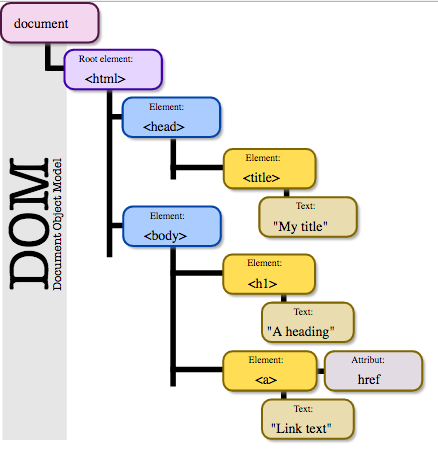
\includegraphics[trim=0cm 0cm 0cm 0cm, clip=true, width=0.5\textwidth]{img/DOM}};
\end{tikzpicture}
\caption{DOM Eredua. Iturria: \newline
\href{http://upload.wikimedia.org/wikipedia/commons/5/5a/DOM-model.svg}{http://upload.wikimedia.org/wikipedia/commons/5/5a/DOM-model.svg}.}
\label{fig:DOM}
\end{figure}

\section{DOM aldatzen JS bidez}

Demagun \ref{fig:ariketaDOM}. irudiko DOM zuhaitza dugula. Bertan, JS erabiliz, hirugarren paragrafoaren (\hl{<p>}) testua aldatu nahi dugu, \textquotedbl{}estás\textquotedbl{} jarri ordez, \textquotedbl{}zaude?\textquotedbl{} ager dadin. Nola egin?

\index{getElementById()}
Lehenengo \textit{hiru} izeneko identifikatzailea duen objektua atzituko dugu,
\index{innerHTML} \hl{document.getElementById()} metodoaz. Metodo horrek DOM zuhaitza zeharkatuko du parametro gisa pasatu diogun identifikatzailea bilatuz. Identifikatzailea bakuna denez, soilik elementu bat aurkituko du. Objektu horrek hainbat metodo eta atributu izango ditu, adibidez \textquotedbl{}innerHTML\textquotedbl{} atributua, objektuaren barruko HTMLa atzitu edo editatzeko aukera emango diguna. Beraz, \textquotedbl{}estás\textquotedbl{} hitza \ref{list:ariketaDOM}. listatuko kodearekin lortu beharko genuke. Probatuko dugu ea egia den...

\begin{figure}[ht]
	\centering
\begin{tikzpicture}
\node[anchor=south west,inner sep=0] (image) at (0,0)
   {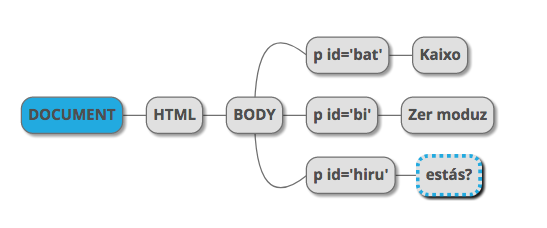
\includegraphics[trim=0cm 0cm 0cm 0cm, clip=true, width=0.5\textwidth]{img/DOMAriketa}};
\end{tikzpicture}
\caption{DOM interfazea ulertzeko ariketaren testuingurua.}
\label{fig:ariketaDOM}
\end{figure}


\begin{lstlisting}[language=JavaScript,numbers=none, label={list:ariketaDOM}, caption={getElementById erabil dezakegu DOM zuhaitzeko objektu bat atzitzeko.}]
let osagai = document.getElementById("hiru");
osagai.innerHTML = "zaude?";
\end{lstlisting}

\section{Nola txertatu JS script bat zure orrian}
Aurreko kodea index.html izeneko orri batean txerta dezakegu. Bi modu daude, \textit{inline} deritzona edo erreferentzia gisa. \index{inline}

\begin{lstlisting}[language=JavaScript,label={list:inlinejs}, caption={\textit{inline} izeneko moduan kodea zuzenean txertatzen da <script> etiketen artean. Ikus: \href{https://codesandbox.io/s/4-gaia-dom-k701t?file=/index.html}{https://codesandbox.io/s/4-gaia-dom-k701t?file=/index.html}}.]
<!DOCTYPE html>
<html lang="eu-es">
  <head>
    <meta charset="utf-8" />
    <script>
      let osagai = document.getElementById("hiru");
      osagai.innerHTML = "zaude?";
    </script>
  </head>
  <body>
    <p id="bat">Kaixoooo</p>
    <p id="bi">Zer moduz</p>
    <p id="hiru">estás?</p>
  </body>
</html>
\end{lstlisting}

\begin{lstlisting}[language=HTML,label={list:referencejs}, caption={JS kodea erreferentziaz ere txerta dezakegu. Horretarako, JS fitxategiaren izena pasatuko diogu <script> etiketari, src atributuan}.]
<!DOCTYPE html>
<html lang="eu-es">
  <head>
    <meta charset="utf-8" />
    <script src="scripta.js"></script>
  </head>
  <body>
    <p id="bat">Kaixoooo</p>
    <p id="bi">Zer moduz</p>
    <p id="hiru">estás?</p>
  </body>
</html>
\end{lstlisting}

Bi kode zati horiek probatuz gero, funtzionatzen ez dutela ikusiko dugu (ikus \ref{fig:no-onload}. irudia). Zergatik? Nabigatzaileak ikusi eta exekutatu duen lehenengo gauza (kodea irakurriz goitik hasita) <head> blokean dagoena delako. Bertan gure <script>-a exekutatu du, baina oraindik ez du orriaren gorputza (body-a) kargatu! Hori dela eta, ezin du aldaketarik egin. Izan ere, kontsola irekitzen badugu, honako errorea ikusiko dugu:

\begin{lstlisting}[language=JavaScript,numbers=none]
Uncaught TypeError: Cannot set property 'innerHTML' of null at (index):9
\end{lstlisting}
    
Alegia, nabigatzailea saiatu da osagaia aurkitzen \textit{document.getElementById("hiru")} eginez, baina ez du ezer topatu. Beraz, \textit{osagai = null} da, eta, hortaz, 
\textit{osagai.innerHTML = "zaude?";} egiten saiatzean, errorea.

\index{onload}
Nola konpondu? Nola esan diezaiokegu nabigatzaileari JavaScript kodea orriaren gorputza kargatu eta gero exekutatu behar duela? Horretarako jaio zen \hl{onload} gertaera-kudeatzailea. Azter dezagun hurrengo atalean.

\begin{figure}[ht]
	\centering
\begin{tikzpicture}
\node[anchor=south west,inner sep=0] (image) at (0,0)
   {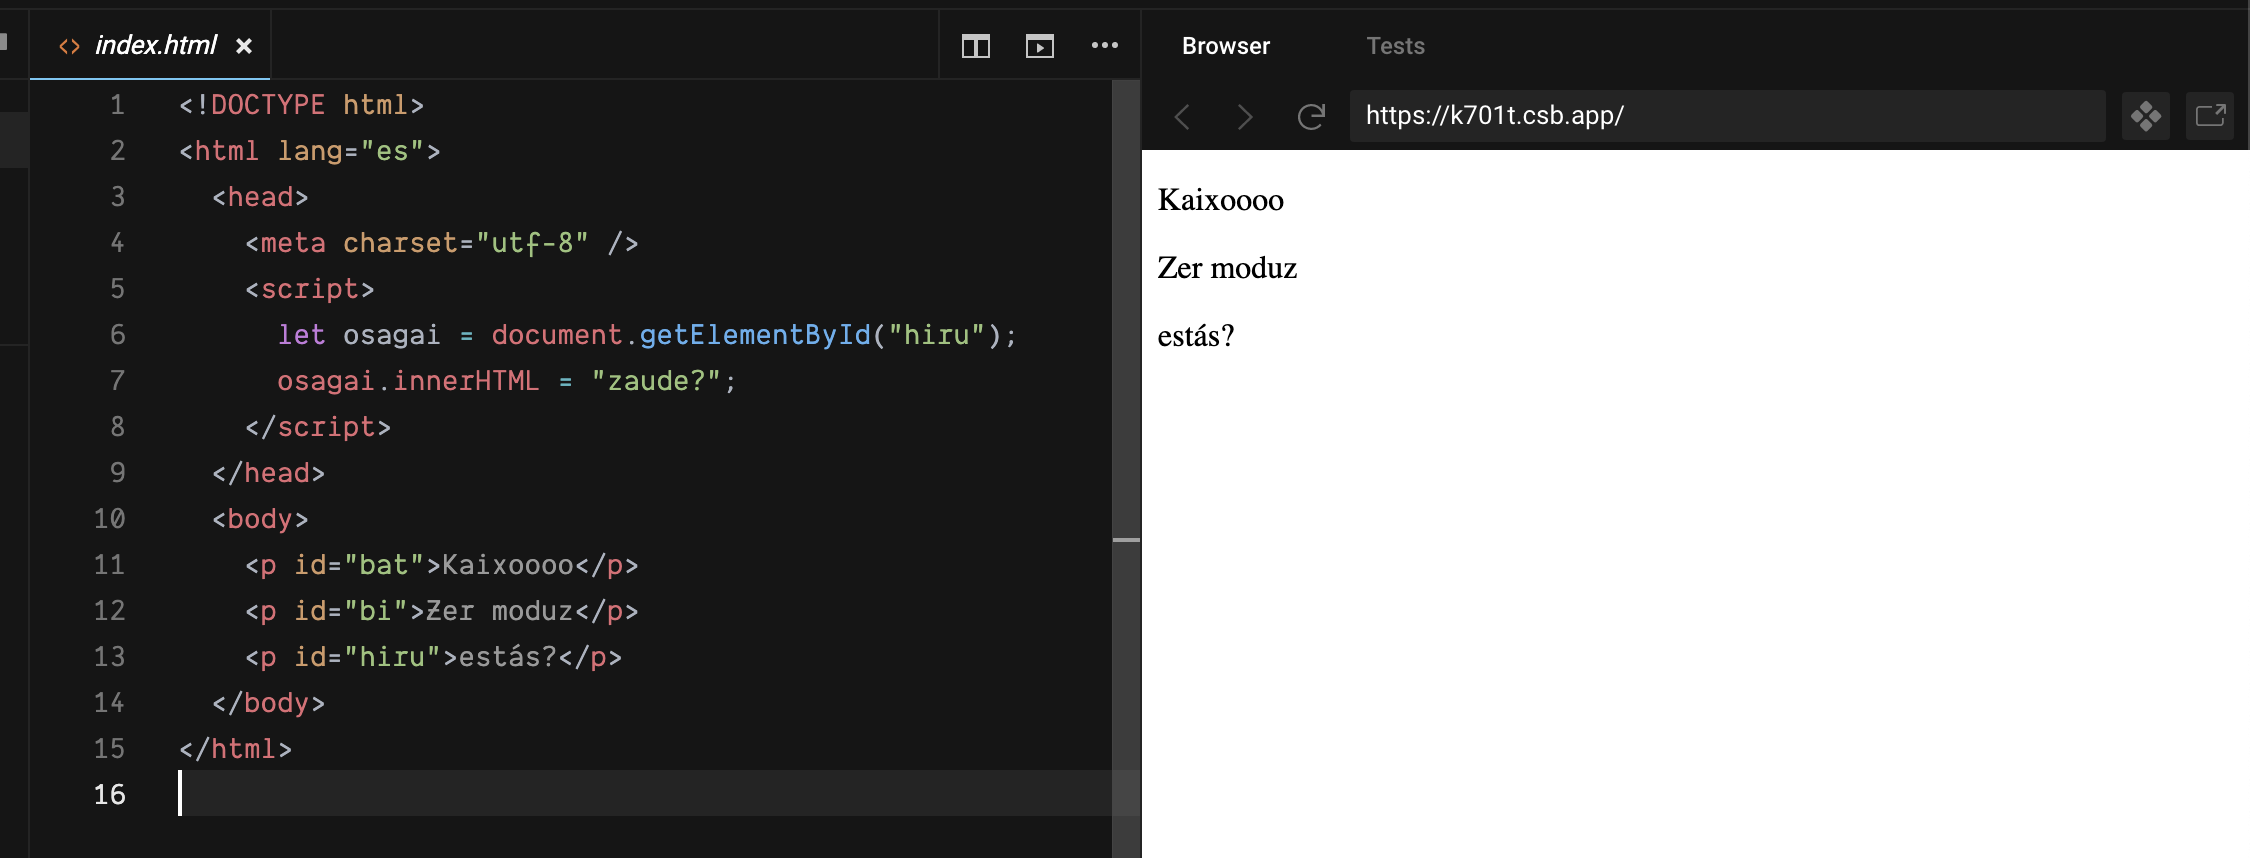
\includegraphics[trim=0cm 0cm 0cm 0cm, clip=true, width=1.0\textwidth]{img/4gaia-no-onload.png}};
\end{tikzpicture}
\caption{DOM edukia aldatzen saiatu gara, baina ez dugu lortu. Zergatik izango ote da... Gai honetan  azalduko dugu.}
\label{fig:no-onload}
\end{figure}

\subsection{onload gertaera-kudeatzailea}

\begin{lstlisting}[language=HTML,label={list:onloadjs}, caption={window.onload egitean gertaera-kudeatzaile bat ezartzen ari gara. Kasu honetan kudeatzailea orriaren edukia kargatu ostean exekutatu egin behar dela esaten ari gara. Ikus: \href{https://codesandbox.io/s/4-gaia-onload-x7wkr?file=/index.html}{https://codesandbox.io/s/4-gaia-onload-x7wkr?file=/index.html}}.]
<!DOCTYPE html>
<html lang="eu-es">
  <head>
    <meta charset="utf-8" />
    <script>
      function edukiaAldatu() {
        let osagai = document.getElementById("hiru");
        osagai.innerHTML = "zaude?";
      }
      window.onload = edukiaAldatu;
    </script>
  </head>
  <body>
    <p id="bat">Kaixoooo</p>
    <p id="bi">Zer moduz</p>
    <p id="hiru">estás?</p>
  </body>
</html>
\end{lstlisting}


\textit{Window} objektuak onload gertaera-kudeatzailea dauka, besteak beste (\textit{window.onload}). Horri esker nabigatzailearen portaera kudea dezakegu. Zehazki, orriaren edukia kargatzen bukatzen denean, \textit{loaded} gertaera altxatuko da. Gertaera hori antzeman eta \hl{edukiaAldatu} izeneko funtzioarekin tratatu nahi dugula esaten ari gara lerro honekin:

\begin{lstlisting}[language=JavaScript, numbers=none]
   window.onload = edukiaAldatu;
\end{lstlisting}

Noski, DOM edukia aldatzeko prestatuta genuen kodea orain \hl{edukiaAldatu} izeneko funtzioan sartu dugu:

\begin{lstlisting}[language=JavaScript]
 function edukiaAldatu() {
        let osagai = document.getElementById("hiru");
        osagai.innerHTML = "zaude?";
      }
\end{lstlisting}

Eta orain bai, dena ondo dabil (ikus \ref{fig:onload}. irudia). Gertaera mota ezberdin interesgarri askoz gehiago daude. Izan ere, horretarako beste gai bat bereziki prestatu dugu liburu honetan (ikus \textbf{6. Gertaerak} kapitulua).

\begin{figure}[ht]
	\centering
\begin{tikzpicture}
\node[anchor=south west,inner sep=0] (image) at (0,0)
   {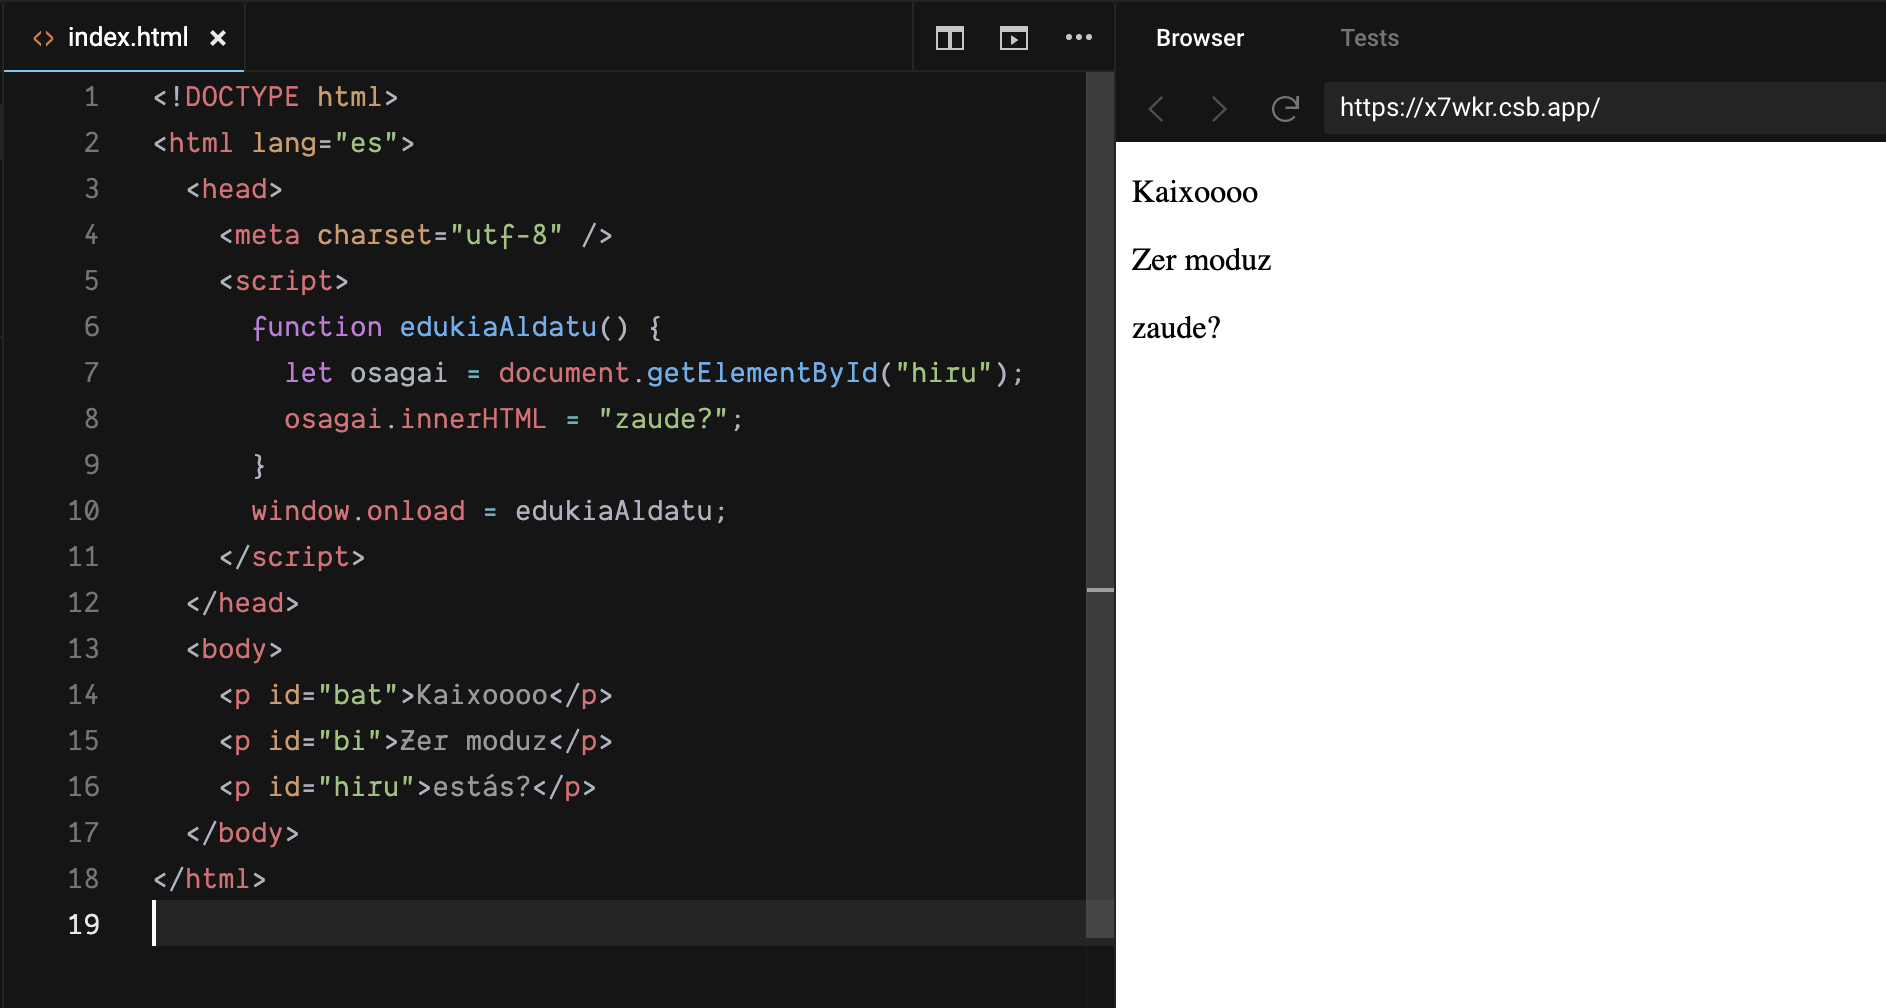
\includegraphics[trim=0cm 0cm 0cm 0cm, clip=true, width=1.0\textwidth]{img/4gaia-onload.png}};
\end{tikzpicture}
\caption{DOM edukia aldatzeko, lehenengo eta behin, orriaren edukia kargatu behar da. Hori lortzeko \textit{window.onload} gertaera-kudeatzailea prestatu dugu.}
\label{fig:onload}
\end{figure}


\section{Ariketak}

Esteka honetan \href{https://labur.eus/WOXzZ}{https://www.dropbox.com/s/7kq7nm8j6m3o9zh/initializr.tgz?dl=1} hurrengo ariketa egiteko beharrezkoak diren fitxategiak aurkituko
dituzu. Jaitsi, destrinkotu eta zure nabigatzailean
index.html orria ireki.

Bertan, webgune baten HTML kodea ematen zaizu. Zure eginbeharra: JS \mbox{script} baten bidez orri nagusian dagoen goiburua ordezkatu, "Uno", "Dos", \mbox{\textquotedbl{}Three\textquotedbl{}} katearen ordez \textquotedbl{}Bat\textquotedbl{}, \textquotedbl{}Bi\textquotedbl{}, \textquotedbl{}Hiru\textquotedbl{} katea ager dadin.

\begin{figure}[ht]
	\centering
\begin{tikzpicture}
\node[anchor=south west,inner sep=0] (image) at (0,0)
   {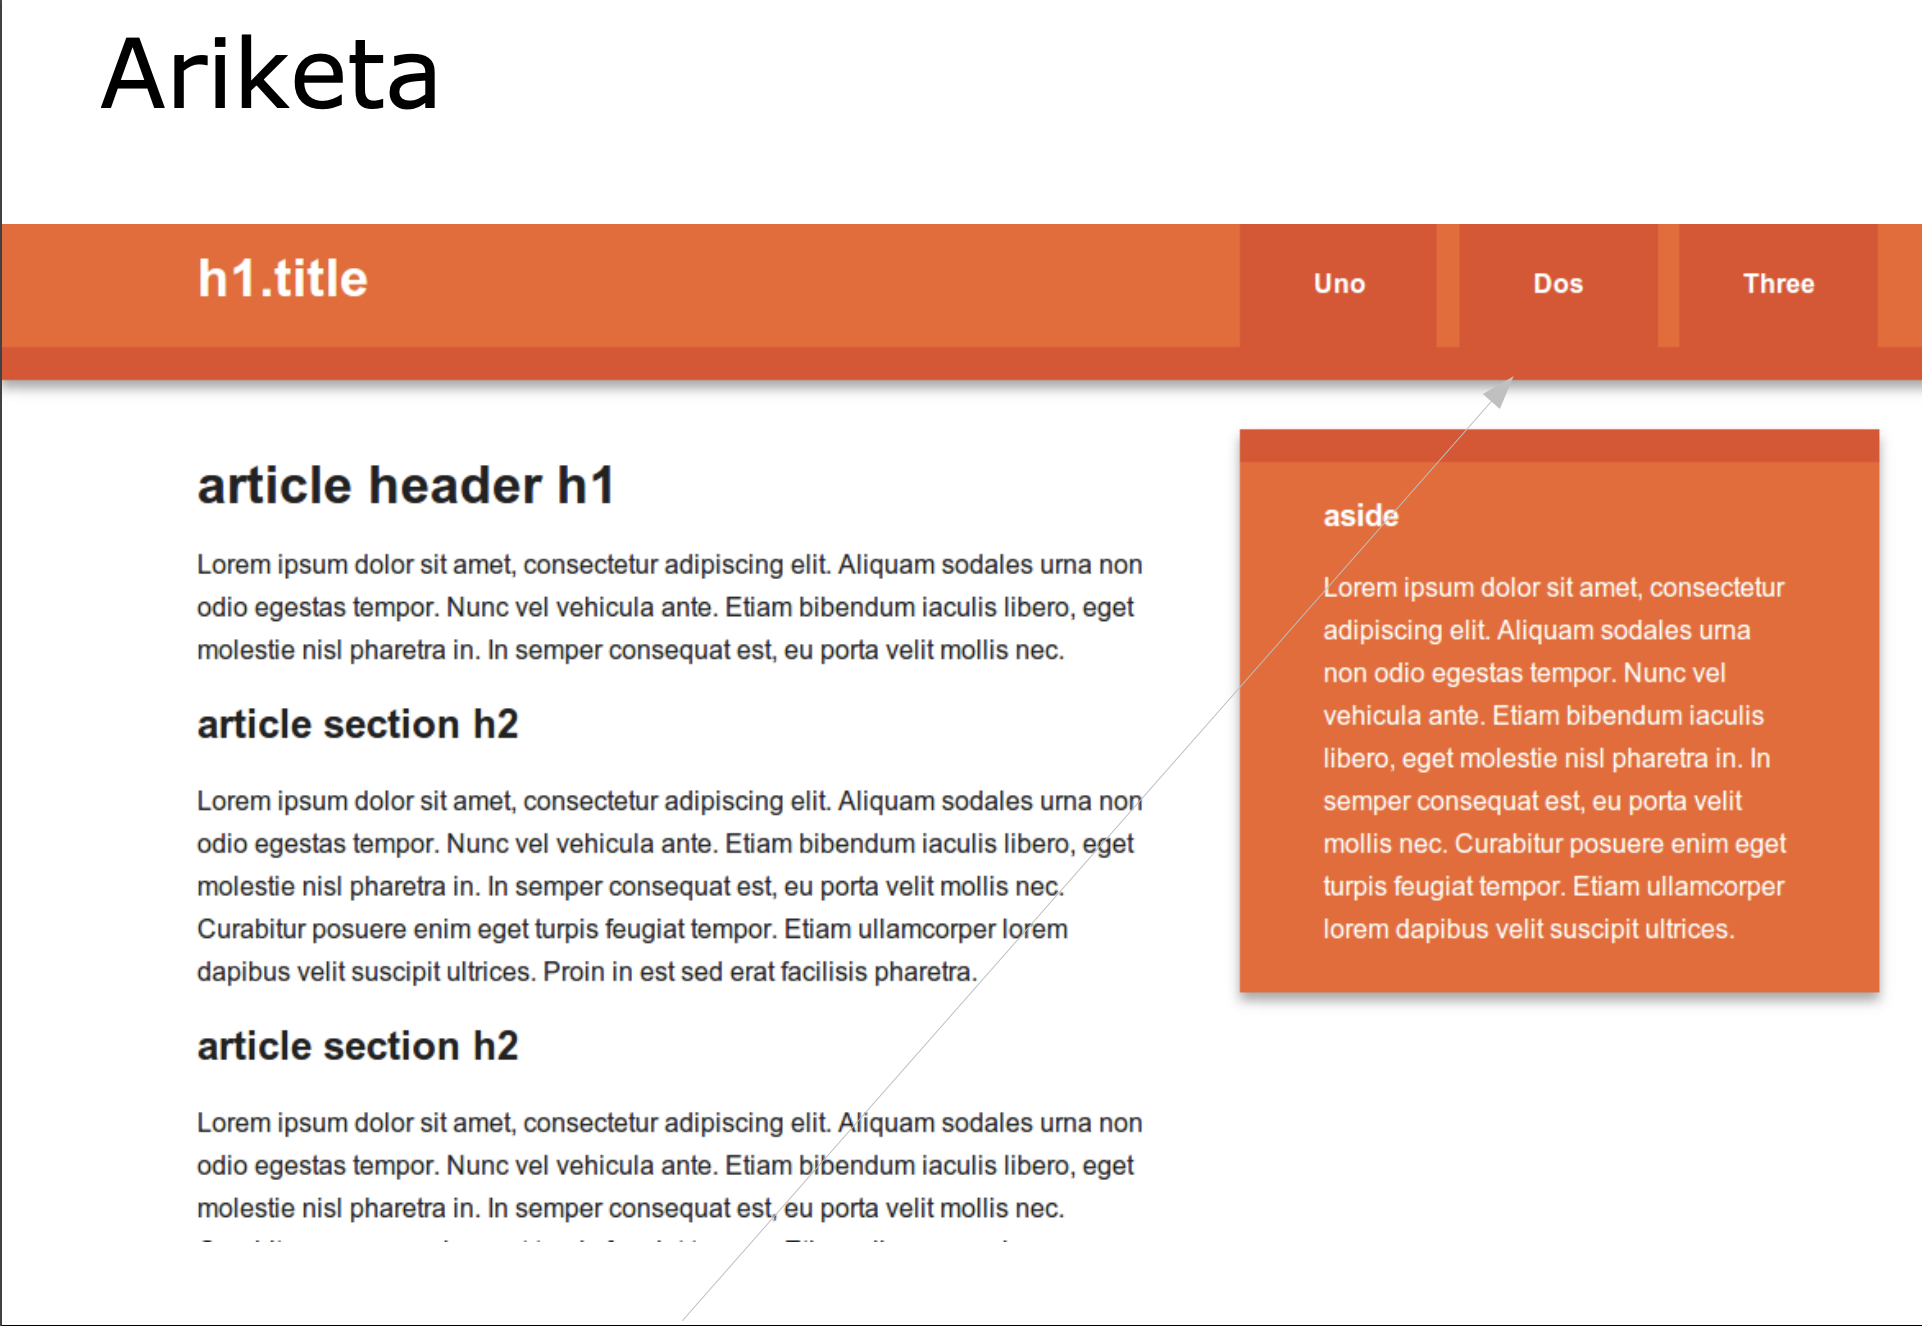
\includegraphics[trim=0cm 0cm 0cm 0cm, clip=true, width=.75\textwidth]{img/dom_ariketa.png}};
\end{tikzpicture}
\caption{DOM edukia aldatzeko JS bat prestatu beharko duzu.}
\label{fig:onload}
\end{figure}
%% 5. OOP
\chapter{Objektuetara zuzendutako programazioa JavaScript-en}

\section{Klaseak JavaScript-en}
JavaScript ez da berez objektuetara zuzendutako programazio (OZP) lengoaia bat, baizik prototipoetan oinarritutakoa. Azken paradigma hori erabilita badago objektuak, herentzia, klaseak, etab. sortzea. Alegia, posible da objektuetara zuzendutako programazio-paradigmari jarraitzea, JavaScript-en helburua beste bat bada ere. Dena den, OZPa hain arrakastatsua bilakatu da JSn, non \index{ECMAScript}\index{ES2015} ECMAScript 2015\footnote{\href{https://262.ecma-international.org/6.0/}{https://262.ecma-international.org/6.0/}} bertsioan klaseak modu erraz batean programatzeko sintaxia onartu baitzen. Sintaxi berri horren bidez, klaseak, objektuak eta klaseen arteko herentzia inplementatzeko kodea erraztu egiten da erabat.

\subsection{Klaseen erazagupena}

Lauki izeneko klase bat erazagutzeko honako egiturari jarraituko diogu:

\index{class}

\begin{lstlisting}[language=JavaScript, numbers=none]
class Lauki {
  constructor(altuera, zabalera) {
    this.altuera = altuera;
    this.zabalera = zabalera;
  }
}
\end{lstlisting}

\index{constructor}\index{this}
Adibidean, Lauki klaseak eraikitzaile metodo bat dauka, \hlc[lightgray]{constructor} izenekoa (eraikitzailea beti deituko da \textit{constructor}). Barruan bi atributu deklaratu dira: altuera eta zabalera. Ohart zaitez atributuak erazagutzeko \hl{this} gako-hitza erabili dela, hots, \textit{this.altuera} eta \textit{this.zabalera}. Atributu hauen balioak esleitzeko, eraikitzaileari  parametro gisa pasatu dizkiogun aldagaien balioak erabili ditugu.

\index{new}
Berez, JSn, klase (\hl{class}) bat funtzio berezi bat besterik ez da. Funtzio horri \hl{new} gako-hitza erabiliz deitzen badiogu, funtzio horrek irudikatzen duen klasea instantziatuko dugu, objektua sortuz. Adibidez, Lauki klaseko laukia izeneko objektu bat instantziatzeko:

\begin{lstlisting}[language=JavaScript, numbers=none]
let laukia = new Lauki(3,4);
\end{lstlisting}

Funtzio arruntetan gertatzen den lez, klase-espresioak ere erabil daitezke:
\begin{lstlisting}[language=JavaScript, numbers=none]
let laukiKlasea = class Lauki {
  constructor(altuera, zabalera) {
    this.altuera = altuera;
    this.zabalera = zabalera;
  }
};

let laukia = new laukiKlasea(3,4);
\end{lstlisting}

\subsection{Get metodoak}
\index{get()}
\index{set()}

Hurrengo adibidean \textit{zabalera()} metodoa \hlc[lightgray]{get} hitzaz apaindu dugu. \hlc[lightgray]{get} gako-hitza da, sintaxia errazteko beste teknika bat. Horrela, \textit{laukia.zabaleraKalkulatu()} bezalako deia erabili ordez, zuzenean \textit{laukia.zabalera} erabili ahalko dugu. Gauza bera \hl{set} metodo bereziarekin. \hl{set} metodo bat erazagutuz, posible da balio bat esleitzea edozein atributuri modu laburrean (adib. \textit{laukia.altuera = 10;})

\begin{lstlisting}[language=JavaScript, numbers=none]
class Lauki {
  constructor(altuera, zabalera) {
    this.altuera = altuera;
    this.zabalera = zabalera;
  }

  set altuera(balioBerria) {
     this.altuera = balioBerria;
  }
  
  get zabalera() {
    return this.zabaleraKalkulatu();
  }

  zabaleraKalkulatu() {
    return this.altuera * this.zabalera;
  }

}
const laukia = new Lauki(5, 10);
console.log(laukia.zabalera); // (get metodoari deitu ondoren, emaitza=50)
laukia.altuera = 2; // set 
console.log(laukia.zabalera); // (get metodoari deitu ondoren, emaitza=20)

\end{lstlisting}

\subsection{Herentzia}

\index{herentzia}
\index{extends}
\index{ES2015}
Herentzia inplementatzeko sintaxia ere erraztu egin du ES2015 estandarrak, \hlc[lightgray]{extends} gako-hitzari esker.

\begin{lstlisting}[language=JavaScript, numbers=none]
class Karratu extends Lauki {
   zabaleraKalkulatu(){
       return this.altuera**2;
   }
   get alde() {
      return this.altuera;
   }
}

let karratu = new Karratu(10,10);
console.log(karratu.alde); // 10
console.log(karratu.zabalera); // 100

\end{lstlisting}

Ohart zaitez \textit{Karratu} klaseko \hl{zabaleraKalkulatu()} metodoan. Gainidatzitako metodo bat da, berez bere gurasoa (Lauki klasea) duen metodoa deuseztatu eta Laukiak bere metodo propioa inplementatzen du. Karratu klaseak \textit{set zabalera()} metodoa ere badu, Lauki klasetik heredatu egin duelako.

\section{Ariketak}

 Objektuetara zuzendutako programazioa erabili beharko duzu hainbat ariketa \newline JavaScript-en programatzeko.

\index{map()}
\index{filter()}
\index{reduce()}
\index{=>}
\index{gezi funtzioa}
\index{arrow}
\begin{enumerate}
\item ES6 sintaxia erabiliz, inplementatu Puntu izeneko klase bat, bi dimentsioko espazioan dagoen puntu bat irudikatzen duena. Puntu batek bi atributu ditu, \hl{x} eta \hl{y}, metodo eraikitzailetik pasatuko dizkiogunak. \textit{batu()} izeneko metodo bat ere badu, parametro gisa beste puntu bat hartzen duena eta emaitza gisa bi puntuen batura itzultzen duena. Alegia, beste puntu berri bat bueltatzen du, non x balioa bi puntuen x balioen batura den (eta gauza bera y puntuari dagokionez).

Beraz, kode hau exekutatzean: 

\begin{lstlisting}[language=JavaScript, numbers=none]
console.log(new Puntu(1, 2).batu(new Puntu(2, 1)))
\end{lstlisting}

Pantailan honako emaitza jaso behar dugu:
\begin{lstlisting}[language=JavaScript, numbers=none]
Puntu{x: 3, y: 3}
\end{lstlisting}

\item Gehitu \textit{hurrengoa()} izeneko metodo bat kontagailu objektuari. Metodo horrek \hl{kont} aldagaiaren uneko balioa itzuli behar du eta unitate batean handitu (erabili \hl{++} eragilea)
\begin{lstlisting}[language=JavaScript, numbers=none]
let kontagailu = {
 kont: 0
 [zure kodea hemen]
}
console.log(kontagailu.hurrengoa())
// -> 0
console.log(kontagailua.hurrengoa())
// -> 1
console.log(kontagailu.hurrengoa())
// -> 2
\end{lstlisting}

\item 
\index{programazio funtzionala}
map(), filter() eta reduce() programazio funtzionalean asko erabiltzen diren array klaseko hiru metodo dira. Webgune honetan \href{https://medium.com/poka-techblog/simplify-your-javascript-use-map-reduce-and-filter-bd02c593cc2d}{https://labur.eus/vGIW4} (medium.com) ikus ditzakezu metodo horien oinarrizko erabileraren adibideak. Horren inguruan zenbait ariketa proposatzen dira.

Honako objektu literala emanik (\hl{biltegia} izenekoa):
\begin{lstlisting}[language=JavaScript, numbers=none]

const biltegia = [
 {mota: "garbigailua", balioa: 5000},
 {mota: "garbigailua", balioa: 650},
 {mota: "edalontzia", balioa: 10},
 {mota: "armairua", balioa: 1200},
 {mota: "garbigailua", balioa: 77}
]

let guztiraGarbigailuenBalioa = zure kodea hemen;

console.log ( guztiraGarbigailuenBalioa ); // 5727 erantzuna espero da
\end{lstlisting}

Erabili \hl{filter()} eta \hl{reduce()} biltegiko garbigailuen balio totala lortzeko. 

\item Gezi funtzioa (\textit{arrow function})  \hl{=>} ES6 estandarrak ekarri duen eta oso preziatua  den funtzioa  bat da. Irakurri gehiago beraren inguruan hemen:  \newline \href{https://www.sitepoint.com/es6-arrow-functions-new-fat-concise-syntax-javascript/}{https://labur.eus/1XZv0} (sitepoint.com).

Jarraian, moldatu hurrengo kodea, \hl{arrow} funtzioa erabili dezan:

\begin{lstlisting}[language=JavaScript, numbers=none]
biltegia.forEach( function(item) {
console.log(item.balioa);
});
\end{lstlisting}

\item Egin hirugarren ariketaren errefaktorizazioa, \textit{arrow} funtzioa erabil dezan.


\end{enumerate}


% 6. Gertaerak
\chapter{Gertaerak eta gertaera-kudeatzaileak}

Web orri baten barruko elementuen egoera aldatzean, gertaerak altxatzen dira. Adibidez, botoi baten gainean klik egitean, botoiaren egoera aldatu dela adierazteko, nabigatzaileak gertaera bat altxatuko du \index{onclick}(\textit{onclick} gertaera, hain zuzen ere). Edo orri baten elementu guztiak kargatzen bukatzean, \index{onload}\textit{onload} gertaera altxatuko da. Gertaerak tratatu nahi izanez gero, gertaera-kudeatzaile bat programatu beharko dugu. Ezezkoan, ez dugu ezer egin behar, alegia, gertaera altxatuko da, baina ez badu inork tratatzen, ez da ezer gertatuko.


\section{Gertaera motak}

Adibideetan ikusi dugun bezala, bi gertaera mota daude: erabiltzaileak sortutakoak (botoi baten gainean klik egin, sagua mugitu, leihoa handitu, tekla bat sakatu...) eta sistemak automatikoki sortutakoak (orri baten elementuak kargatzen bukatzean, bideo bat bistaratzeko prest dagoenean, errore bat gertatzen denean...).  Azter ditzagun horrelako gertaera zehatzen adibide batzuk.

\subsection{Erabiltzaileak sortutako gertaerak}

Maiz erabiltzen diren gertaera mota hauen adibideak:
\begin{itemize}
\item onclick (saguarekin elementu baten gainean klik egitean)
\item \index{onmouseover} onmouseover (sagua elementu baten gainean jartzean)
\item \index{onblur} onblur (elementu batek fokua galtzen duenean)
\item \index{onfocus} onfocus (elementu batek fokua hartzen duenean)
\item \index{ondrag} ondrag (elementu bat arrastatzean)
\item \index{onkeypress} onkeypress (tekla bat sakatzean)
\end{itemize}


\subsection{Sistemak sortutakoak}
  Maiz erabiltzen diren gertaera mota hauen adibideak:

\begin{itemize}
\item \index{onload} onload (elementu bat kargatzen bukatzean)
\item \index{oncanplay} oncanplay (elementu multimedia bat kargatu eta ikusi edo jo dezakegunean)
\item \index{onoffline} onoffline (konexioa galtzean)
\end{itemize}


\section{Nola kudeatu gertaerak JavaScript-en}

Hiru modu ezberdin daude gertaerak JSn kudeatzeko. Kudeatzaileak HTML kodean txertatuz, gertaeraren iturri-osagaiaren gainean kudeatzaile bat zuzenean definituz edo \index{addEventListener} metodo generikoa erabiliz.

\subsubsection{JavaScript HTML kodean txertatu}

Elementuaren ostean \textit{onclik} atributuan zer funtzio exekutatu nahi dugun zehaztuko dugu, adibidez:

\begin{lstlisting}[language=JavaScript,numbers=none]
<button onclick="alert('Hello world');">
  Sakatu hemen
</button>
\end{lstlisting}

\subsubsection{Osagaiaren gainean kudeatzailea zuzenean definitu}

Askotan gomendagarria da gertaera-kudeatzaileak JS fitxategi batean gordetzea eta funtzio horiek osagaiaren izena erabiliz zehaztea, honelako patroiari jarraituz:

\begin{lstlisting}[language=JavaScript,numbers=none]
osagaia.gertaera = function()
{
   // gertaera kudeatzeko kodea
}
\end{lstlisting}

Adibidez, aurreko adibide bera honela programatu dezakegu:
\begin{lstlisting}[language=JavaScript,numbers=none]
  botoia.onclick = function()
  {
    //
   // gertaera kudeatzeko kodea
   };
\end{lstlisting}

\index{addEventListener}
\subsubsection{addEventListener metodo generikoa erabiliz}

\textit{addEventListener} metodoak 2 parametro hartzen ditu\footnote{addEventListener metodoa gainkargatuta dago, alegia, 2 parametro baino gehiagoko bertsioak ere baditu. addEventListener eta removeEventListener inguruan informazio gehiago MDNn aurkituko duzu (\href{https://developer.mozilla.org/en-US/docs/Web/API/EventTarget/addEventListener}{https://developer.mozilla.org/en-US/docs/Web/API/EventTarget/addEventListener}).}, tratatu nahi dugun gertaeraren izena eta funtzio-kudeatzailearen izena, eskema honi jarraituz:

\begin{lstlisting}[language=JavaScript,numbers=none]
osagaia.addEventListener('gertaera', funtzioa);
\end{lstlisting}

Gauza bera gertaera-kudeatzaile bat elementu batetik ezabatu nahi izanez gero. Kasu honetan, \textit{removeEventListener} metodoa erabiliko dugu.

Adibidez, botoiaren gainean sakatzean funtzio bat exekutatzeko:

\begin{lstlisting}[language=JavaScript,numbers=none]
botoia.addEventListener('click', funtzioarenizena);
\end{lstlisting}

Eta momentu batean esleipen hori kendu nahiko bagenu, \index{removeEventListener}\textit{removeEventListener} erabiliko genuke:

\begin{lstlisting}[language=JavaScript,numbers=none]
botoia.removeEventListener('click', funtzioarenizena);
\end{lstlisting}


\section{Adibide praktikoa}

Demagun \ref{fig:gertaerakadibidepraktikoa}. irudian ikusten den bezalako webgune bat dugula. Irudian zenbait errezetaren argazkiak agertuko dira, sekuentzian. Gure helburua errezeta baten gainean klik egitean, kontsolan mezu bat agertzea da.

\begin{figure}[ht]
	\centering
\begin{tikzpicture}
\node[anchor=south west,inner sep=0] (image) at (0,0)
   {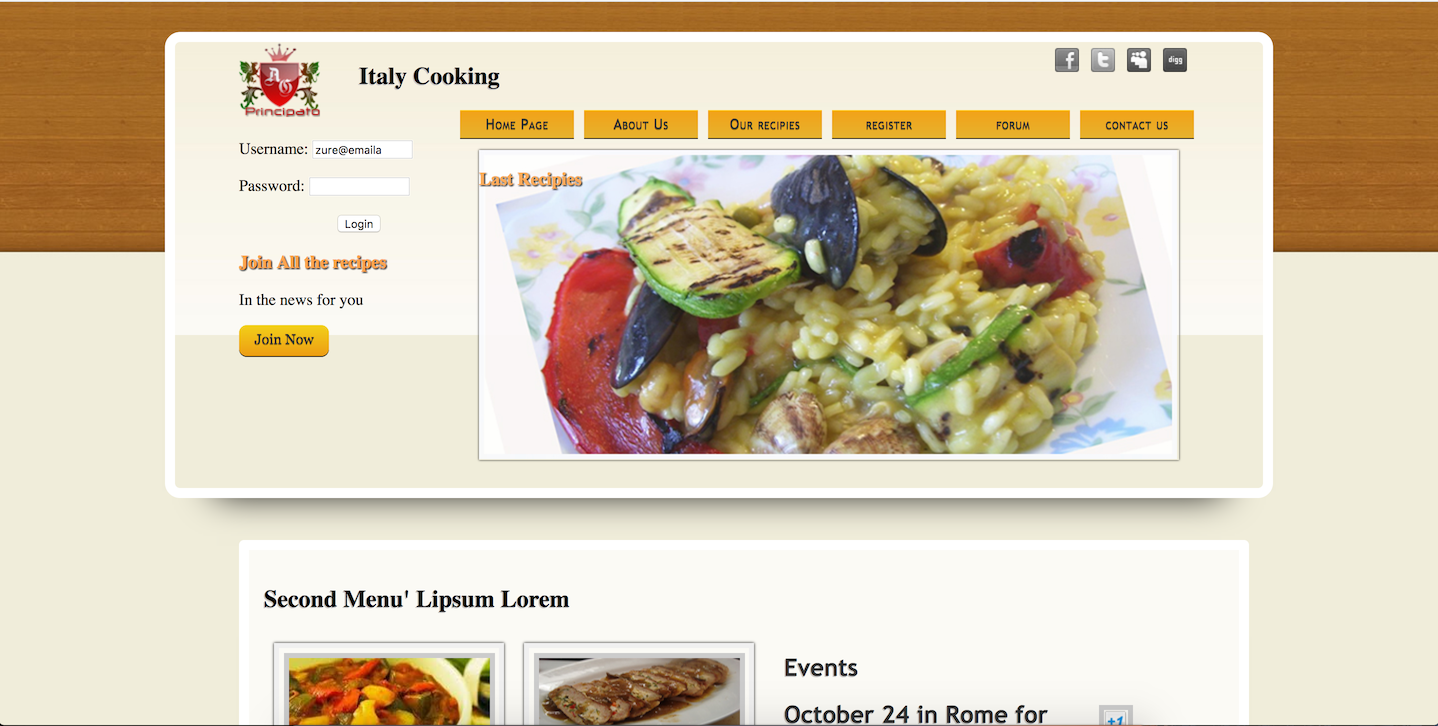
\includegraphics[trim=0cm 0cm 0cm 0cm, clip=true, width=0.75\textwidth]{img/errezetak}};
\end{tikzpicture}
\caption{Gertaerak: adibide praktikoak.}
\label{fig:gertaerakadibidepraktikoa}
\end{figure}




\begin{lstlisting}[language=JavaScript,numbers=none]
function kudeatzaileakHasieratu()
{
   let irudia = document.getElementById('irudia');
   irudia.onclick = function() {
      console.log("Irudia sakatu duzu");
  }
}


window.onload = kudeatzaileakHasieratu;
\end{lstlisting}

\index{onload}
Garrantzitsua da \textit{window.onload}-en gertaera-kudeatzailea zehaztea. Horrela egingo ez bagenu, eta zuzenean \hl{kudeatzaileakHasieratu} metodoari deituko bagenio,
posible litzateke irudia oraindik kargatu gabe egotea, eta, hortaz, \hl{getElementById()} egitean \textit{null} aurkitzea.

\subsubsection{Gertaerak kudeatzen: \textit{onblur}, \textit{onfocus}}

Aurreko irudian ikusten dugun inprimakian erabiltzailearen datuak (email-helbide eta pasahitza) eskatzen dira. Helbide elektroniko bat testu-eremu batean idatzi behar duela gogorarazteko trikimailu bat erabil dezakegu \textit{onblur} gertaeraz baliatuz. Erabiltzaileak email-helbidea ez badu oraindik idatzi eta horretarako dagoen testu-eremua hutsik badago, orduan \textquotedbl{}zure@emaila\textquotedbl{} bezalako argibidea idatziko dugu bertan testu-eremu horrek fokua galtzean (\textit{onblur}). Berriz, testu-eremu horrek berriro fokua hartzen duenean (\textit{onfocus}), eta oraindik email-helbidea idatzi gabe badu, balioa hustu egingo dugu. 

\begin{lstlisting}[language=JavaScript]
let erabiltzaile = document.getElementById('erabiltzaile');
erabiltzaile.value = 'zure@emaila';

erabiltzaile.onfocus = function(event){
  let input = event.target
  if (input.value == 'zure@emaila'){
    erabiltzaile.value = '';
 }
}

erabiltzaile.onblur = function(event){
	let input = event.target
	if (input.value == ''){
	    erabiltzaile.value = 'zure@emaila';
  	}
}

\end{lstlisting}

\subsubsection{Gertaerak kudeatzen: \textit{onchange}}

Erabiltzaileak aukera-zerrenda (\textit{combobox}) bateko aukeraren bat hautatzean \textit{onchange} gertaera altxatzen da. Zerrendan hainbat osagai daude <select> etiketaren  barruan:

\begin{lstlisting}[language=HTML,numbers=none]
    <option value="rice">Arroza</option>
    <option value="mushrooms">Txanpinoiak</option>
\end{lstlisting}

Hurrengo adibidean \textit{zerrendaKudeatzaile} funtzio bat prestatu dugu gertaera horri erantzuteko. Zehazki, aukeratu den elementuaren balioa (\textit{value} atributuan dagoena), elementu horren indizea zerrendan \index{\textit{selectedIndex}}(selectedIndex) eta aukera horren testua (adibidez, Arroza).

\begin{lstlisting}[language=HTML5]
let item = document.getElementById('combobox');
item.addEventListener('change', zerrendaKudeatzaile);

function zerrendaKudeatzaile(event){
   let item = event.target
   console.log(item.value); // rice
   console.log(item.selectedIndex);  // 2
   console.log(item.options[item.selectedIndex].text); // Rice with mushrooms
}

<select name="GoMenu" style="width:159px" id="combobox">
<option selected="selected">Select a recipe</option>
<option class="_self" value="spaghetti">Spaghetti with aubergine</option>
<option class="_self" value="rice">Rice with mushrooms</option>
<option class="_self" value="rolls">Rolls with polenta</option>
<option class="_self" value="chicken">Chicken Hunter</option>
<option class="_self" value="tortiglioni">Tortiglioni filled</option>
<option class="_self" value="swordfish">Smoked swordfish</option>
<option class="_self" value="pumpkins">Stuffed pumpkins</option>
</select>
\end{lstlisting}

\subsubsection{Gertaerak kudeatzen: \textit{onsubmit}}
Inprimaki baten \textit{onsubmit} gertaera inprimakiaren ``Bidali'' botoian sakatzean altxatzen da. Gertaera hori erabil dezakegu inprimakian sartu diren balioak zuzenak diren edo ez egiaztatzeko (zerbitzarira bidali baino lehen). Horretarako, funtzio bat esleituko diogu \textit{onsubmit} kudeatzaileari. Funtzio horrek parametroak aztertu eta denak zuzenak badira, \hl{true} bueltatu behar du. \hl{False} kontrako kasuan.

\begin{lstlisting}[language=JavaScript]
let inprimakia = document.getElementById('inprimakia');
inprimakia.onsubmit = function(){
console.log("Bidali botoian klikatu duzu");
 // eremuak baliostatu. 
// Baten bat bete gabe balego, false itzuli
// Bestela, true itzuli
return false;
}
\end{lstlisting}

\subsubsection{Gertaerak kudeatzen: \textit{onchange} \textit{range}}

\index{range}
Inprimaki baten \textit{range} motako osagaiak \textit{onchange} gertaera altxatzen du erabiltzaileak tiraderatik tira egiten duenean alde batera edo bestera. \textit{Range} osagaiaren balioa une oro ikusi ahal izateko, gertaera horri honako kudeatzailea esleitu diezaiokegu:

\begin{lstlisting}[language=JavaScript]
<form>
 <input type='range' min=1 max=100 step=1 id='tartea'>
 </form>

 <div id='balioa'></div>
 <script>
let kudeatzaileHasieratu = function()
{
   let tartea = document.getElementById('tartea');
   tartea.addEventListener('change', balioaBistaratu)

   function balioaBistaratu( event ){
       let tartea = event.target
       document.getElementById('balioa').innerHTML = tartea.value;
   }
} 

window.onload = kudeatzaileaHasieratu;
</script>

\end{lstlisting}

\subsubsection{Gertaerak kudeatzen: \textit{setTimeout}, \textit{setInterval}}

\index{setTimeout}
\index{setInterval}
Bukatzeko, aldiro-aldiro funtzio bat exekutatu nahiko bagenu (adibidez, 5 segundoan behin funtzio bat exekutatu nahiko bagenu), oso interesgarria litzateke \textit{setInterval} metodoa. Bi parametro hartzen ditu, exekutatu nahi den funtzioaren izena eta zer maiztasunez exekutatu nahi dugun, milisegundotan.

Adibidez, idatzi() izeneko funtzioa 5 segundoan behin exekutatu nahiko bagenu:
\begin{lstlisting}[language=JavaScript]
function idatzi() {
       console.log("Idazten..." + new Date());
}
let erlojua = setInterval(idatzi, 5000);
\end{lstlisting}

Beste batzuetan ez dugu aldiro-aldiro exekutatu nahiko, baizik eta behin bakarrik X segundo pasa ostean. Horretarako, \textit{setTimeOut} funtzioa erabiliko dugu. Adibidez, idatzi funtzioa 5 segundo barru exekutatzeko (ez aldiro, baizik eta soilik behin, 5 segundo barru):

\begin{minipage}{\linewidth}
\begin{lstlisting}[language=JavaScript]
function idatzi()
{
      console.log("Idazten...." + new Date());
}
let reloj = setTimeOut(idatzi, 5000);
\end{lstlisting}
\end{minipage}

\section{Ariketak}

Gai honen inguruan planteatzen diren ariketak webgune baten gainean egin behar dira. Jaitsi beharrezkoak diren txantiloia \href{https://www.ikasten.io/html5/ariketak/fitxategiak/06_txantiloia.zip}{https://labur.eus/2DWcm} (ikasten.io) eta  irudiak \href{https://www.ikasten.io/html5/ariketak/fitxategiak/06_irudiak.zip}{https://labur.eus/BiAms} (ikasten.io) eta jarrai iezaiezu ariketa egiteko argibideei.

\begin{itemize}
    \item JavaScript erabiliz dinamikoki alda daiteke <div> etiketa baten barruan zehazten den irudia. Adibidez, \ref{fig:gertaerak-ariketa-1}. irudian dugun webgunearen kasuan, errezetaren irudia alda dezakegu.
    
    \begin{figure}[ht]
	\centering
\begin{tikzpicture}
\node[anchor=south west,inner sep=0] (image) at (0,0)
   {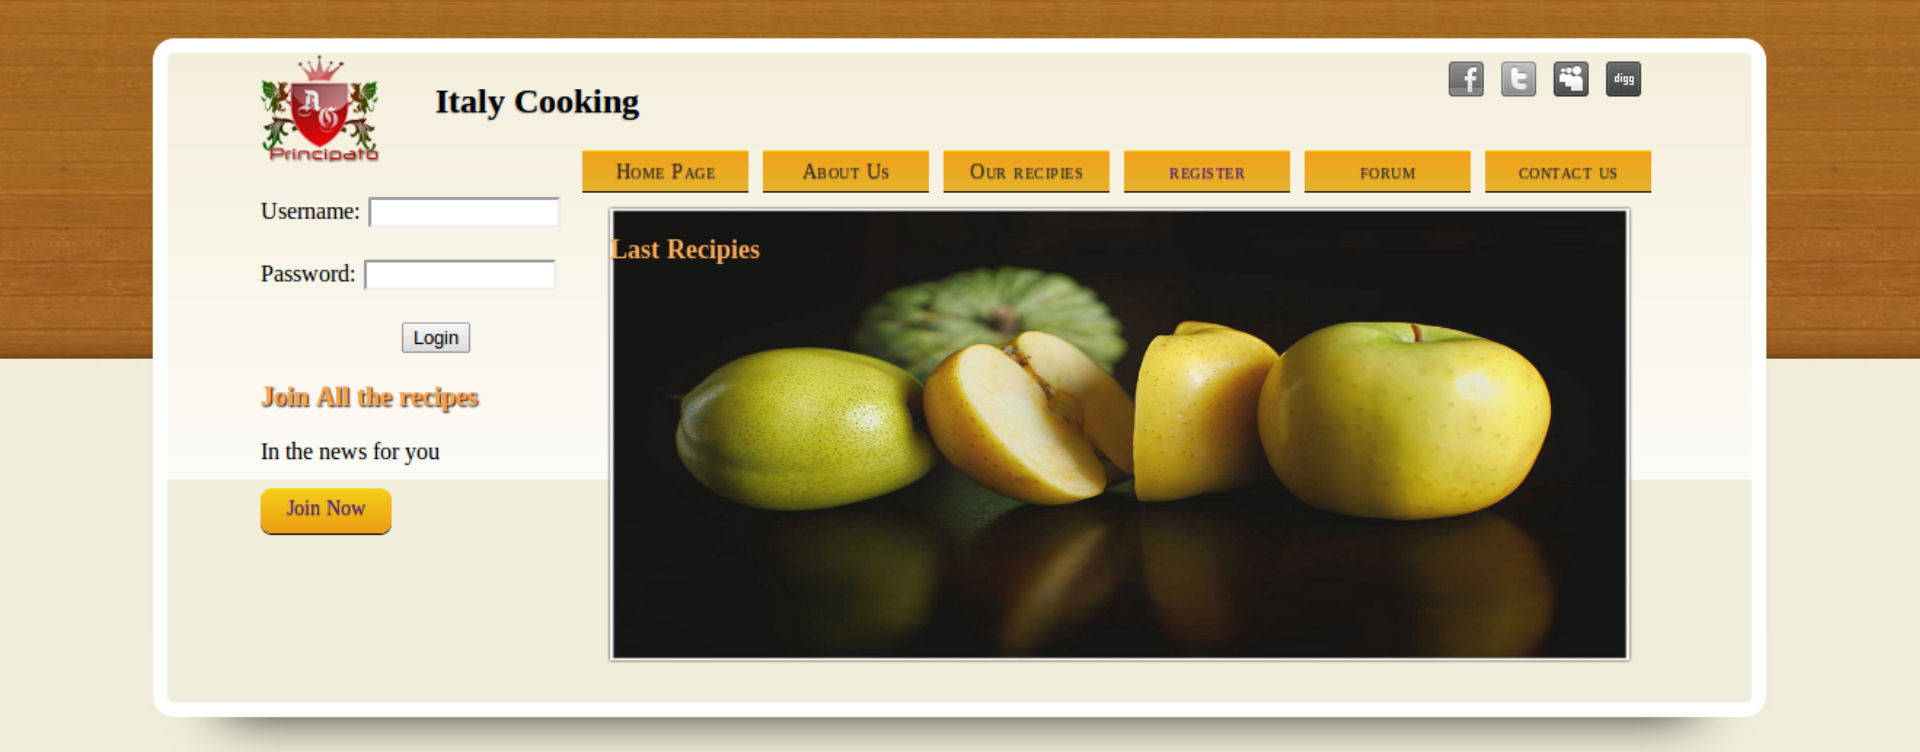
\includegraphics[trim=0cm 0cm 0cm 0cm, clip=true, width=0.75\textwidth]{img/gertaerak/gertaerak_ariketa_2.png}};
\end{tikzpicture}
\caption{Gertaerak: ariketaren hasierako egoera.}
\label{fig:gertaerak-ariketa-1}
\end{figure}

Horretarako, honako kodea erabiliko dugu:

\begin{lstlisting}[language=JavaScript,numbers=none]
let irudia = document.getElementById("irudia")
irudia.style.backgroundImage = "url(irudiak/irudiberria.jpg)"
\end{lstlisting}

Ariketa honetan irudi hori 5 segundoan behin aldatzea  eskatzen da (ikus \ref{fig:gertaerak-ariketa-2}. irudia). Sei irudiz osatutako array batetik hartuko dugu hurrengo irudia. Alegia, gai honetan ikusi dugun webgunean oinarrituta, beharrezkoa den JavaScript kodea programatu irudi guztiak sekuentzian bistaratzeko (5 segundoan behin). Erabiltzaileak irudiaren gainean sakatzen badu, irudien animazioa eten egin behar da. Irudiaren gainean ez badu sakatzen, 6. irudiaren ondoren berriro lehenengoa bistaratuko da, sekuentziari jarraituz (ikus: \href{http://www.youtube.com/watch?v=aaoNMmnfGD4}{http://www.youtube.com/watch?v=aaoNMmnfGD4}).

\begin{figure}[ht]
	\centering
\begin{tikzpicture}
\node[anchor=south west,inner sep=0] (image) at (0,0)
   {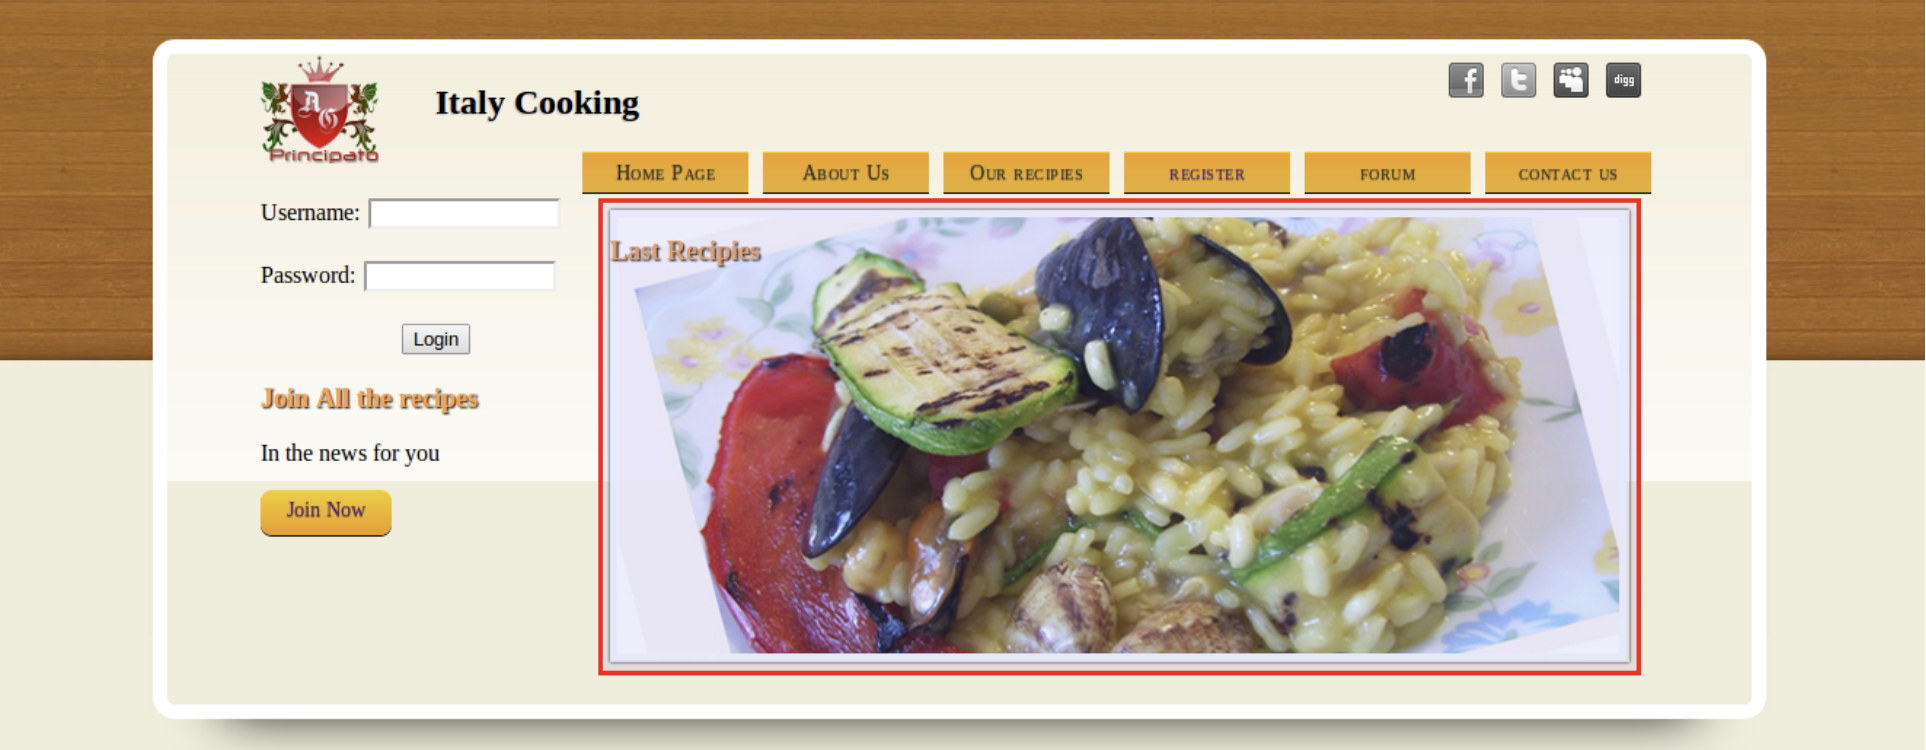
\includegraphics[trim=0cm 0cm 0cm 0cm, clip=true, width=0.75\textwidth]{img/gertaerak/gertaerak_ariketa_1.png}};
\end{tikzpicture}
\caption{Gertaerak: ariketaren helburu-egoera.}
\label{fig:gertaerak-ariketa-2}
\end{figure}




\end{itemize}

%% 7. JSON & AJAX & Promesak
\chapter{Datuen komunikazio asinkronoa: JSON, Ajax eta Promesak}

Nabigatzaileek kanpoko zerbitzariei web orriak eta gainontzeko elementuak eskatzeko HTTP protokoloa erabiltzen dute. Besterik ezean, nabigatzaileak eskaera sinkronoak egiten ditu: orria eskatu eta HTML kodearen zain geratzen da. Jaso ondoren, URLa aldatu eta beste orri bat eskatu ahalko dugu (aurrekoa gainidatziz).

\begin{figure}[ht]
	\centering
\begin{tikzpicture}
\node[anchor=south west,inner sep=0] (image) at (0,0)
   {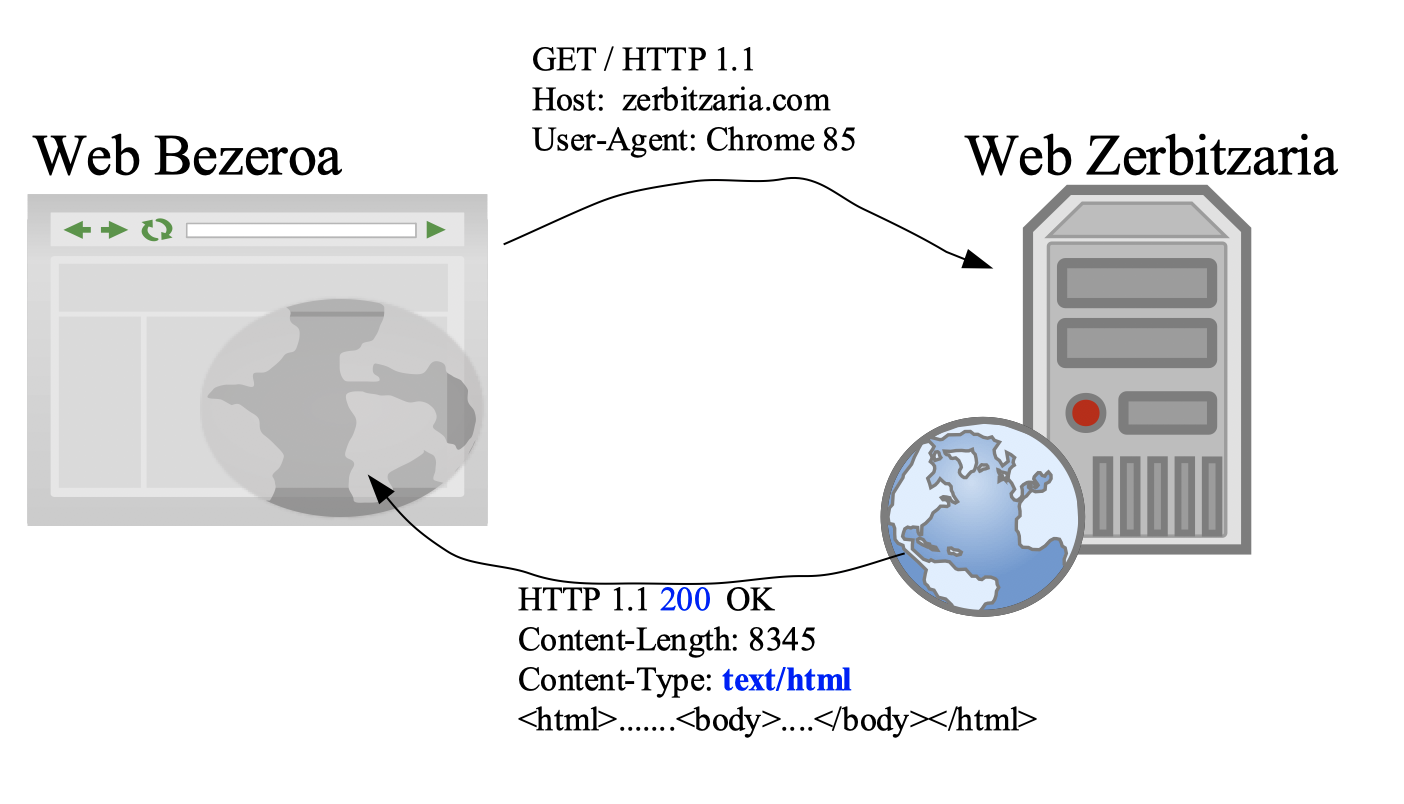
\includegraphics[trim=0cm 0cm 0cm 0cm, clip=true, width=0.75\textwidth]{img/http-protokoloa.png}};
\end{tikzpicture}
\caption{HTTP protokoloa eskaera sinkronoak eta asinkronoak egiteko erabil dezakegu.}
\label{fig:http-protocol}
\end{figure}

Baina batzuetan, behar dugun gauza bakarra ez dira web orri osoak izango, datu gordinak baizik. Are gehiago, batzuetan web orri baten barruan soilik datu zehatz bat bistaratu nahiko dugu, eta datua jasotzean ez dugu web orria zapaldu nahi, baizik eta datu hori pantailan ikusten dugun orriarekin integratu.

Adibidez, demagun Bilbo hiriaren GPS geokokapena non dagoen jakin nahi dugula. OpenWeatherMap izeneko zerbitzu bati, munduko hirien latitudea eta longitudea gordetzen dituen web zerbitzu bati, deitu diezaiokegu horretarako. Irudian ikusten dugun bezala, haren erantzuna ez da HTML formatuan etorriko, \index{JSON}JSON formatuan (JavaScript Object Notation) baizik. Horrez gain, eskaera ez dugu HTTP sinkrono bat erabiliz jaso nahi, baizik eta eskaera asinkrono batekin. Alegia, pantailan dugun orriaren edukia ordezkatu gabe, nabigatzaileak eskaera bat egingo dio OpenWeatherMap zerbitzuari eta JSON erantzuna jasotzean, Bilboko koordenatuak orrian bertan txertatu, dagokion lekuan.

HTTP eskaera asinkrono hauek \index{XHR}XHR (\index{XMLHttpRequest}XMLHttpRequest) edo AJAX \index{AJAX} izenarekin ezagutzen dira.

\begin{figure}[ht]
	\centering
\begin{tikzpicture}
\node[anchor=south west,inner sep=0] (image) at (0,0)
   {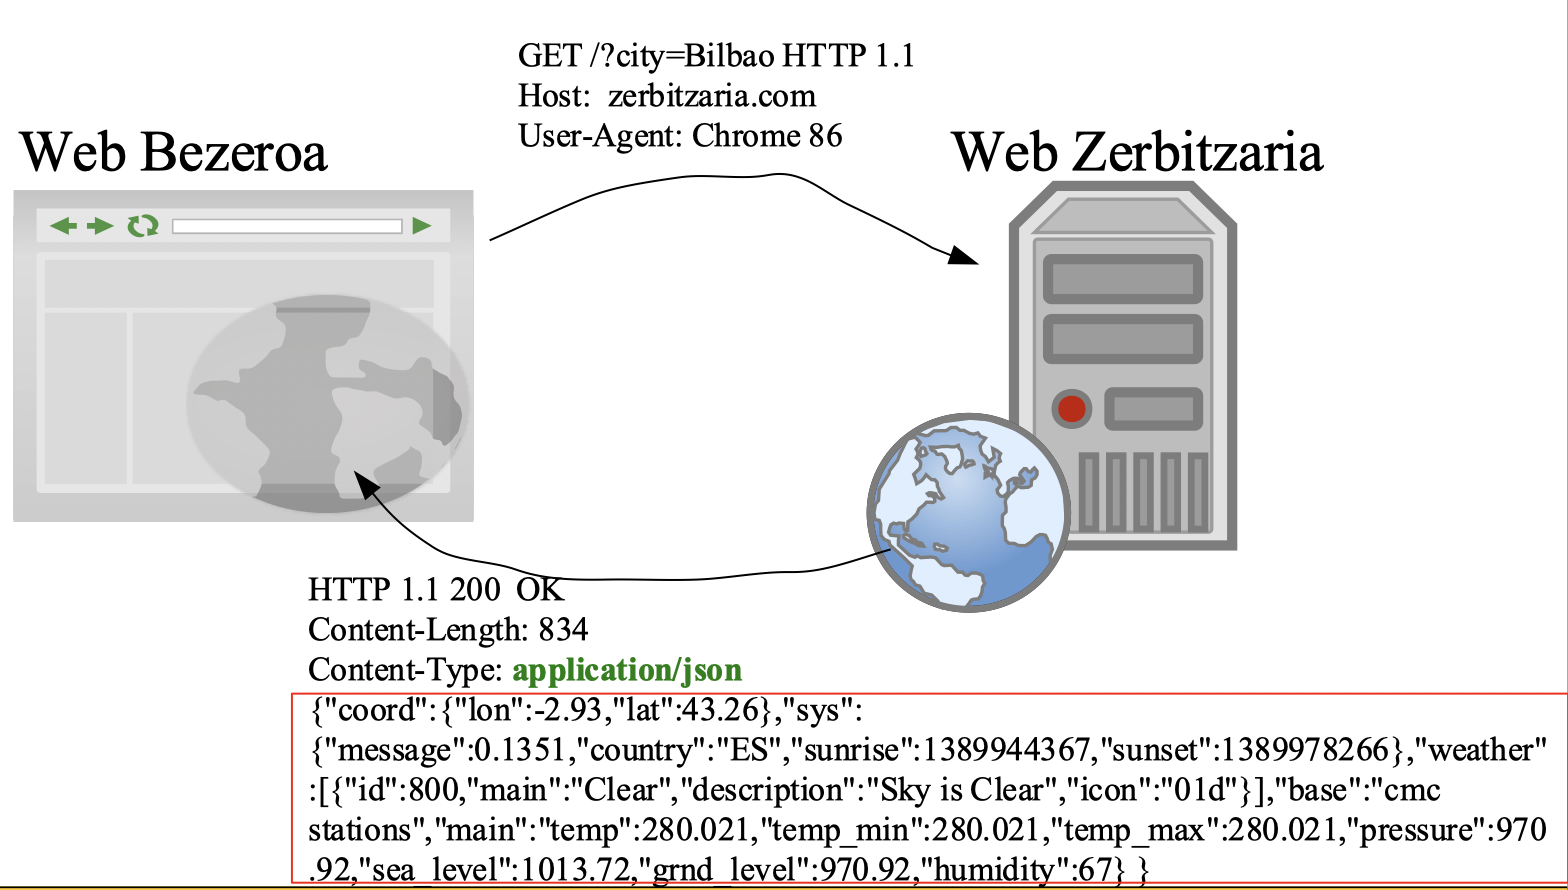
\includegraphics[trim=0cm 0cm 0cm 0cm, clip=true, width=0.75\textwidth]{img/xhr.png}};
\end{tikzpicture}
\caption{HTTP protokoloa erabiliz eskaera asinkronoak egiteari AJAX edo XHR deritzo. Adibidean, XHR dei bat egin diogu web zerbitzariari eta hark erantzuna bidali digu JSON formatuan.}
\label{fig:XHR}
\end{figure}

Adi! \index{XHR} XHR eskaerak egitean ez dugu zertan XML erabili. Hasieran XML Interneteko formatu estandarra bazen ere, gaur egun gehien erabiltzen den formatua JSON da eta, berez, XHR eskaeretan XML edo JSON jaso dezakegu.

Orain dela urte batzuk AJAX edo XHR eskaera bat egiteko kodea nahiko korapilatsua zen:

\begin{minipage}{\linewidth}
\begin{lstlisting}[language=JavaScript]
// zerbitzaria eta eskaera zehaztu
let url = "http://api.openweathermap.org/data/2.5/weather? q=Bilbao,es";

// Eskaera kudeatzeko XHR objektua sortu
let kontsulta = new XMLHttpRequest();

// URL horri eskaera egiteko GET metodoa erabiliko dugula zehaztu
kontsulta.open("GET", url);

//  eskaera asinkronoaren erantzuna kudeatuko duen funtzioa zehaztu
kontsulta.onload = function() {
  if (kontsulta.status == 200) {
    console.log("Arrakastaz egikaritutako kontsulta");
    console.log( kontsulta.responseText );
  }
};
// bukatzeko, eskaera jaurti besterik ez zaigu falta 
kontsulta.send();
\end{lstlisting}
\end{minipage}

AJAX eskaera baten erantzuna JSON formatuan baldin badator ere (ikus \ref{fig:XHR}. irudia), \textit{string} huts bat da. Modu eroso batean tratatu nahi badugu, JSON objektu bihurtu beharko dugu.
Adibidez, aurreko kode zatian, \index{responseText}\textit{kontsulta.responseText} katea JSON objektu bihurtzeko, \index{JSON.parse}\textit{JSON.parse} metodoa erabili beharko dugu.

\begin{verbatim}
    let erantzuna = JSON.parse(kontsulta.responseText);
\end{verbatim}

Gaur egun, kode hori guztia asko laburbil daiteke \index{fetch APIa}\textit{fetch} APIarekin. Izan ere, aurreko AJAX eskaera egiteko eta JSON formatura bihurtzeko, nahikoa litzateke lerro bakar hau exekutatzea (ikus \ref{fig:fetchAPI}. irudia):

\begin{verbatim}
fetch("http://api.openweathermap.org/data/2.5/weather?
q=Bilbao,es").then( r => r.json())
\end{verbatim}


\begin{figure}[ht]
	\centering
\begin{tikzpicture}
\node[anchor=south west,inner sep=0] (image) at (0,0)
   {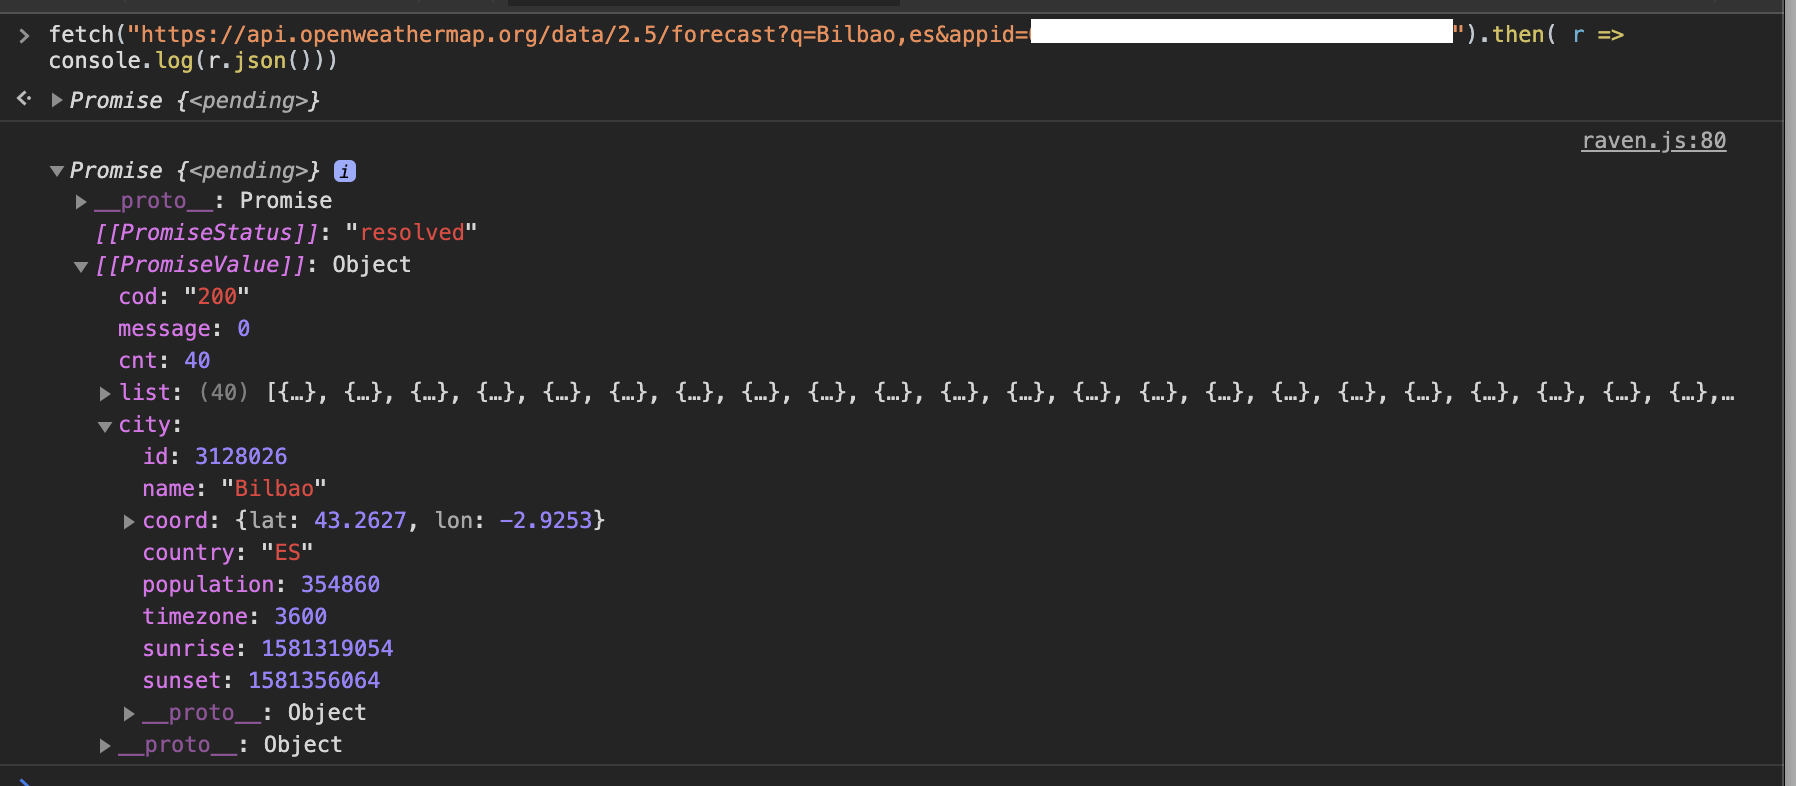
\includegraphics[trim=0cm 0cm 0cm 0cm, clip=true, width=0.75\textwidth]{img/openweatherfetch.png}};
\end{tikzpicture}
\caption{OpenWeatherMap (OWM) zerbitzuari AJAX eskaera bat egiteko HTML5ek eskaintzen duen \textit{fetch} APIa erabil dezakegu. Adi, doako API key bat eskatu beharko baitugu lehenengo OWM webgunean.}
\label{fig:fetchAPI}
\end{figure}

\index{Promise}\index{Promesak}
\section{Promesak}
Promes baten funtzionamendua ondo ulertzeko adibide bat ekarriko dugu. Irudi bat kargatu nahi dugu dinamikoki, promes baten bidez. Irudia deskargatu eta prest dagoenean dokumentuari erantsiko diogu DOM erabiliz, honela:

\begin{lstlisting}[language=JavaScript]
loadImage('https://developers.google.com/web/images/ web-fundamentals-icon192x192.png').
	then( image => document.body.appendChild(image) )
\end{lstlisting}

loadImage() irudia kargatzeko funtzioa da, promes bat itzultzen duena. Promesa betetzean (\textit{then} klausulan) document.body atzitu eta irudia erantsiko diogu .


\begin{lstlisting}[language=JavaScript]
function loadImage(url){
	return new Promise(resolve => {
		const image = new Image();
		image.addEventListener('load', () => {
			resolve(image);
		});
		image.src = url;
		});
}
\end{lstlisting}

loadImage() funtzioak, hortaz, URL bat hartzen du (irudiaren URLa) parametro gisa eta promes bat bueltatzen du. Promesak, aldiz, parametro gisa funtzio bat hartzen du ( \textit{.then} klausularen barruan definitu duguna aurreko kode zatian). Promes batek beti deituko dio parametro gisa jasotzen duen \textit{resolve} funtzioari, promesa betetzen denean.

Gure adibidean, noiz beteko da promesa? Lehenengo irudi bat sortzen dugu (new Image()). Jarraian, gertaera-kudeatzaile bat esleitzen diogu irudiari (image.addEventListener), irudia URLtik jaitsi eta prest dagoenean exekutatuko dena (onLoad). Kudeatzaile horrek deituko dio \textit{resolve} funtzioari. Noiz? image.src = url; komandoak irudia kargatzen bukatzen duenean (irudiaren iturria URLtik jaistean eta prest dagoenean). Ohart zaitez azken komando hori asinkronoa dela, alegia, badakigu noiz hasten den (komandoa exekutatzen hasten denean), baina ez noiz bukatzen den zehazki (denbora gutxiago edo gehiago har dezake irudia deskargatzeko konexio-kalitatearen arabera, adibidez).

Hurrengo irudian (\ref{fig:fetchAPI}. irudian), exekutatu dugun promesaren emaitza irudikatzen da. Zehazki, \hlc[lightgray]{fetch()} metodoaz dei asinkrono bat egin dugu eta promes bat jaso dugu. Promesa betetzean (\textit{fetch().then( r )} klausularen barruan gaudenean, non r jaso dugun erantzuna den)  erantzun bat aurkituko dugu. Erantzun hori JSON formatura bihurtu dugu (r.json() erabiliz). Orain, erantzuna JSON objektua denez, oso modu erosoan trata dezakegu. Adibidez, latitudearen eta longitudearen koordenatuak lortzeko, objektua.city.coord erabiliko genuke. Ikus hurrengo kode zatia:

\begin{lstlisting}[language=JavaScript]
fetch("https://api.openweathermap.org/data/2.5/forecast?
q=Bilbao,es&appid=XXXXXXXXXXXXXX").then( r => r.json()).then( objektua => {
  console.log(objektua);
  console.log(objektua.city.coord);
})
\end{lstlisting}

JavaScript-en edozein objektu JSON formatura bihur dezakegu eta hortik String arrunt batera \index{JSON.stringify}\hl{JSON.stringify} metodoa erabiliz (serializazioa deitzen zaio prozesu horri). Adibidez:

\begin{lstlisting}[language=JavaScript]
let liburu = new Liburu("Dublinés", "Alfonso Zapico", 18);
let jsonLiburua = JSON.stringify(liburu);
// orain jsonLinburua JSON formatuan dagoen String bat da
console.log(jsonLiburua);
// {"izenburua": "Dublinés", "egilea": "Alfonso Zapico",
// "salneurria": 18}
\end{lstlisting}

\section{Fetch APIa}

Fetch APIarekin eskaera asinkronoak egin ditzakegu, bai GET nola POST metodoak erabiliz (besteak beste). Ikus ditzagun adibide batzuk.

\subsection{Fetch APIa GET eskaerak egiteko}

OpenLibrary zerbitzuak eskaintzen duen APIa erabiliz liburu baten datuak jasoko ditugu fetch dei batekin:

\begin{lstlisting}[language=JavaScript]
fetch(
'https://openlibrary.org/api/books? bibkeys=ISBN:0451526538&format=json').
then( r => r.json() ).
then( datuak => { 
 console.log(datuak) 
 })
\end{lstlisting}

fetch egin ondoren, erantzun gordina jasoko dugu r parametroan. Parametro horren edukia JSON objektu bat denez, r.json() erabiliko dugu erantzuna JSON bihurtzeko. Jarraian, datuak izeneko parametroan jasoko dugu JSON objektua eta kontsolatik bistaratuko dugu, honako emaitza jasoz:

\begin{lstlisting}
{"ISBN:0451526538": 
{"bib_key": "ISBN:0451526538", 
"preview": "noview", 
"thumbnail_url": "https://covers.openlibrary.org/b/id/295577-S.jpg",
"preview_url": "https://openlibrary.org/books/OL1017798M/ The_adventures_of_Tom_Sawyer", 
"info_url": "https://openlibrary.org/books/OL1017798M/ The_adventures_of_Tom_Sawyer"
}}
\end{lstlisting}

Erantzun horretan thumbail\_url edo liburu-azalaren irudi txikia eskuragarri izango dugu. Beste \hl{fetch()} dei batekin jaso eta uneko orrian txertatuko dugu (\ref{fig:fetchAPIwebkontsola}. irudia):

\begin{lstlisting}[language=JavaScript]
fetch(
'https://openlibrary.org/api/books? bibkeys=ISBN:0451526538&format=json').
then( r => r.json() ).
then( datuak => { 
     let thumbnail_url = datuak["ISBN:0451526538"].thumbnail_url;
     let irudia = new Image(); irudia.src= thumbnail_url; document.body.appendChild( irudia );
 })
\end{lstlisting}

\begin{figure}[ht]
	\centering
\begin{tikzpicture}
\node[anchor=south west,inner sep=0] (image) at (0,0)
   {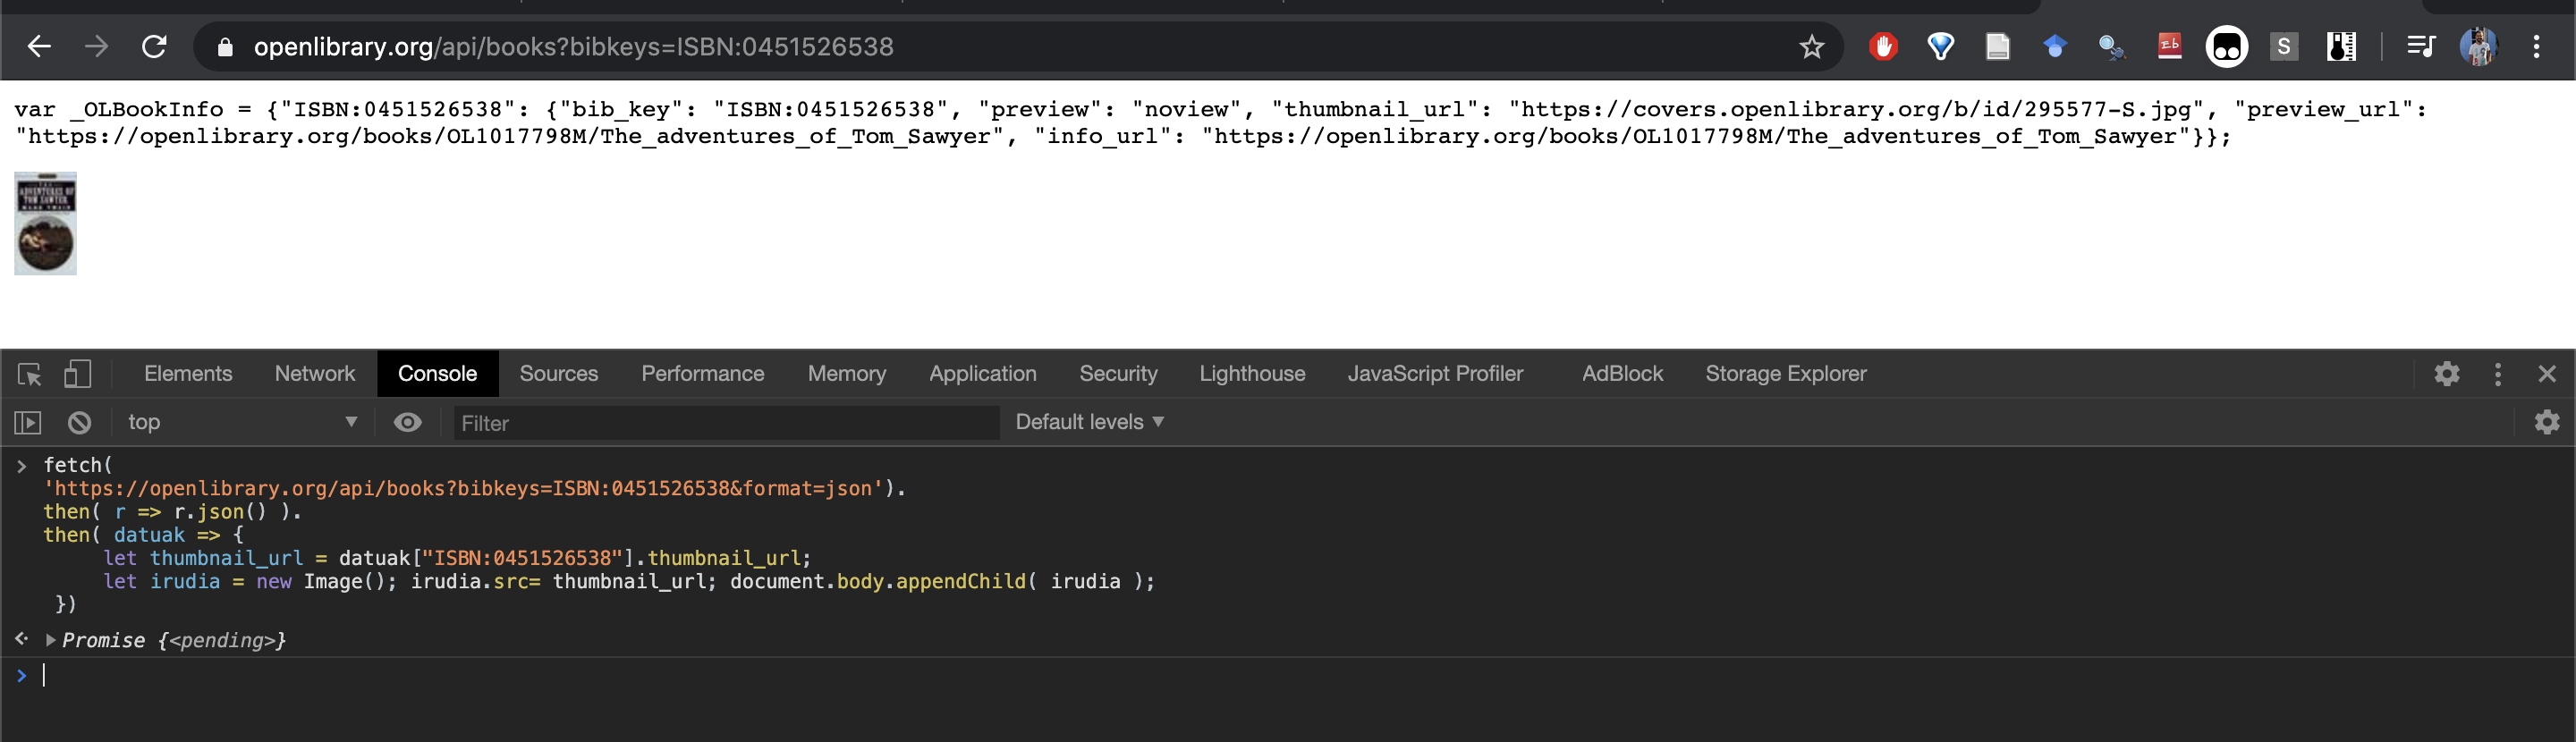
\includegraphics[trim=0cm 0cm 0cm 0cm, clip=true, width=1.0\textwidth]{img/fetch_webkontsola.png}};
\end{tikzpicture}
\caption{Fetch APIa erabiliz API bat kontsultatu eta erantzuna \textit{parseatu} ondoren, bertan zegoen irudi bat dokumentuan txertatu dugu. Probak egiteko nabigatzailearen web kontsola erabili dugu (ikus \ref{sec:webkontsola} atala).}
\label{fig:fetchAPIwebkontsola}
\end{figure}

\subsection{Fetch APIa POST eskaerak egiteko}

Fetch APIa POST eskaerak egiteko ere erabil daiteke. Horretarako, URLaren ondoren JSON objektu gisa parametroak pasa diezazkiokegu, \textit{method} eta \textit{body} atributuetan. 

Adibide gisa, httpbin.org/post helbidera (bidaltzen diogun guztia erantzun gisa errepikatuko du) POST eskaera bat bidaliko dugu, aldagai1=balio1 eta aldagai2=balio2 parametroekin:

\begin{minipage}{\linewidth}
\begin{lstlisting}[language=JavaScript]
fetch("https://httpbin.org/post", 
{ 
 method: 'POST',
 body: 'aldagai1=balio1&aldagai2=balio2'
}).then( resp => resp.text()).
then( erantzuna => console.log(erantzuna))
\end{lstlisting}
\end{minipage}

Eta erantzun gisa, honakoa jasoko dugu:

\begin{lstlisting}[language=JavaScript,numbers=none]
{
  "args": {}, 
  "data": "aldagai1=balio1&aldagai2=balio2", 
  "files": {}, 
  "form": {}, 
  "headers": {
    "Accept": "*/*", 
    "Accept-Encoding": "gzip, deflate, br", 
    "Accept-Language": "eu,en-US;q=0.9,en;q=0.8,es;q=0.7",
    "Cache-Control": "no-cache", 
    "Content-Length": "31", 
    "Content-Type": "text/plain;charset=UTF-8", 
    "Host": "httpbin.org", 
    "Origin": "chrome-search://local-ntp", 
    "Pragma": "no-cache", 
    "Sec-Fetch-Dest": "empty", 
    "Sec-Fetch-Mode": "cors", 
    "Sec-Fetch-Site": "cross-site", 
    "User-Agent": "Mozilla/5.0 (Macintosh; Intel Mac OS X 10_15_4) AppleWebKit/537.36 (KHTML, like Gecko) Chrome/83.0.4103.97 Safari/537.36", 
    "X-Amzn-Trace-Id": "Root=1-5edfaeca-dbf4fb5585f92c45ae2efda3"
  }, 
  "json": null, 
  "origin": "47.63.89.49", 
  "url": "https://httpbin.org/post"
}
\end{lstlisting}

\section{Ariketak}

Gai honetan zenbait teknologia eta teknika berri landu dira. JSON, AJAX, Fetch APIa eta Promesak. Horiek guztiak ondo ulertzeko ezinbestekoa da praktikatzea. 

\begin{enumerate}
    \item GDAX webguneak kriptotxanponen prezioa ezagutzeko API bat eskaintzen du. Adibidez, URL honi deituz \href{https://api.gdax.com/products/btc-eur/ticker}{https://api.gdax.com/products/btc-eur/ticker} \faBitcoin itcoin  baten prezioa (\faEuro urotan) emango digu, JSON formatuan (besteak beste, hainbat datu eskaintzen baititu dei horren erantzunak).
    
    \begin{figure}[ht]
	\centering
\begin{tikzpicture}
\node[anchor=south west,inner sep=0] (image) at (0,0)
   {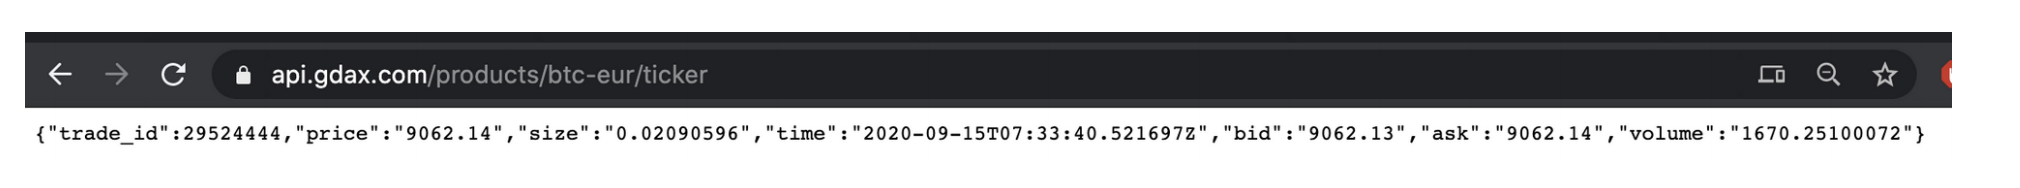
\includegraphics[trim=0cm 0cm 0cm 0cm, clip=true, width=1.0\textwidth]{img/json/json_ariketa_1.png}};
\end{tikzpicture}
\caption{JSON erantzun ezberdina jasoko dugu exekutatzen dugun guztietan, kriptotxanpon baten balioa une oro aldatzen baita.}
\label{fig:jsonariketa1}
\end{figure}

\faBitcoin itcoin baten prezioa dinamikoa da, egunean zehar hainbat aldiz aldatuko da (berez segundoero!).

fetch APIa erabiliz aurreko URLari deitu eta kontsolan idatzi \faBitcoin itcoin baten uneko prezioa.

\item loadImage() metodoa txantiloi gisa erabiliz (gogoratu gai honi dagokion kapituluan azaltzen dela bere funtzionamendua):

\begin{lstlisting}[language=JavaScript,numbers=none]
function loadImage(url){
   return new Promise(resolve => {
      const image = new Image();
      image.addEventListener('load', () => {
         resolve(image);
      });
      image.src = url;
});
}

loadImage('https://developers.google.com/web/images/ irudia.png').
then( image => document.body.appendChild(image) )
\end{lstlisting}

Inplementa ezazu loadAudio(url) izeneko beste funtzio bat, non parametro gisa audio-fitxategi baten URLa ematen zaion eta audio hori memorian kargatzen duen. Funtzioa inplementatu ondoren, dei honen bidez audioa entzun beharko litzateke:

\begin{lstlisting}[language=JavaScript,numbers=none]
loadAudio('https://zerbitzaria.com/audioa.mp3').then( audioa => audioa.play() );
\end{lstlisting}



\end{enumerate}
%% 8. Canvas
\chapter{Canvas, pantailan marrazten}\index{canvas}
Canvas osagaiak oihal edo mihise bat eskaintzen du web orrian edozein marrazketa egin ahal izateko, pixelak, formak edo testua. Canvas erabiliz 60 \textit{frame}/segundoko abiaduran pantaila osoan marraztu dezakegu, animazioak sortuz. Ospe handiko Doom edo Quake bezalako bideo-jokoak HTML5era eraman dira, besteak beste, \textit{canvas} osagaiari esker. 


\begin{figure}[ht]
	\centering
\begin{tikzpicture}
\node[anchor=south west,inner sep=0] (image) at (0,0)
   {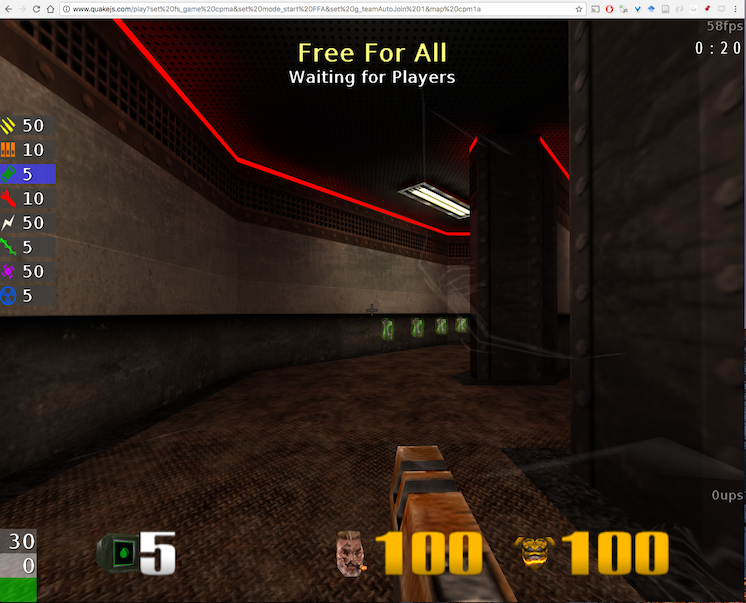
\includegraphics[trim=0cm 0cm 0cm 0cm, clip=true, width=0.75\textwidth]{img/quakejs}};
\end{tikzpicture}
\caption{Canvas eta JavaScript APIak erabiliz Quake bideo-jokoaren bertsio bat nabigatzailean.}
\label{fig:quakejs}
\end{figure}



\section{<canvas> osagaia}
Canvas-en marrazten hasteko, \textit{canvas} (oihala) osagaiaren luzera eta zabalera zehaztu behar ditugu:
\begin{verbatim}
<canvas id="oihala" width="600" height="200"></canvas>    
\end{verbatim}

Jarraian, bertan bi dimentsioko grafikoak marraztu nahi ditugula adieraziko dugu, \hlc[lightgray]{getContext('2d')} \index{getContext()} metodoaren bidez:
\begin{lstlisting}[language=JavaScript,numbers=none]
    let oihala = document.getElementById("oihala");
    let context = oihala.getContext("2d");
\end{lstlisting}

Behin 2D ingurunea prest dugunean, hainbat eragiketa izango ditugu eskuragarri, adibidez, laukizuzen beteak marrazteko \hlc[lightgray]{fillRect()} \index{fillRect} metodoa. Ikus \ref{lst:canvas1}. listatua.


\begin{figure}[ht]
	\centering
\begin{tikzpicture}
\node[anchor=south west,inner sep=0] (image) at (0,0)
   {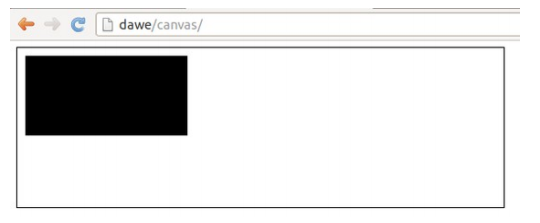
\includegraphics[trim=0cm 0cm 0cm 0cm, clip=true, width=0.75\textwidth]{img/canvas}};
\end{tikzpicture}
\caption{Canvas-en laukizuzen sinplea margotzen.}
\label{fig:canvaslaukia}
\end{figure}


\begin{figure}[ht]
	\centering
\begin{tikzpicture}
\node[anchor=south west,inner sep=0] (image) at (0,0)
   {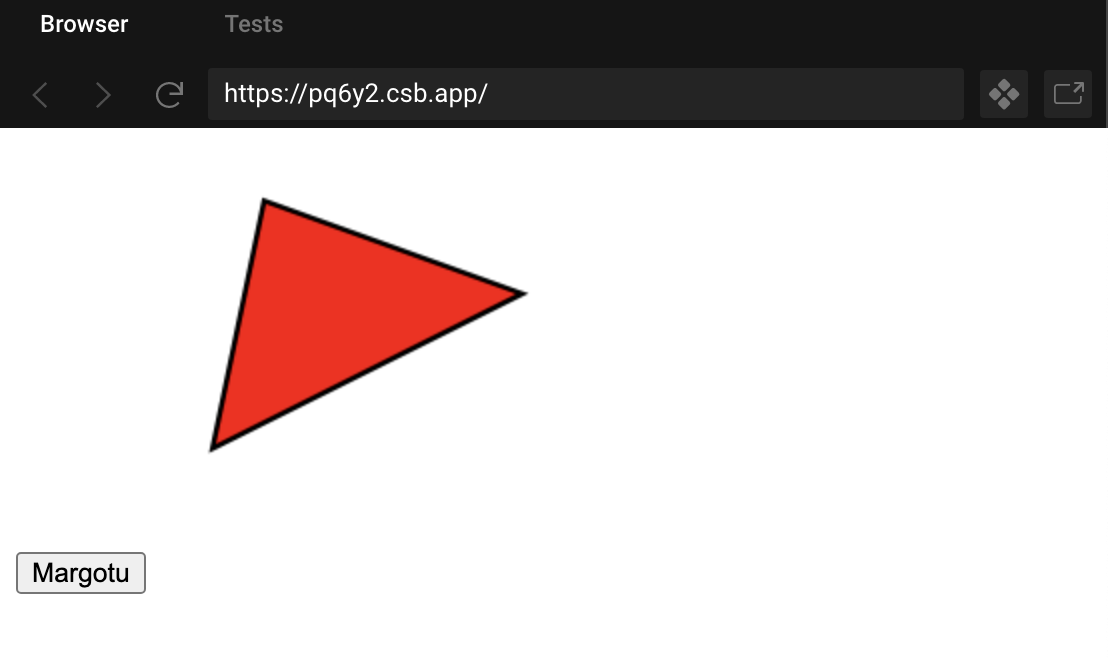
\includegraphics[trim=0cm 0cm 0cm 0cm, clip=true, width=0.75\textwidth]{img/canvas_hirukia.png}};
\end{tikzpicture}
\caption{\textit{Margotu} izeneko botoian sakatzean, canvas-en gorriz betetako hiruki bat margotuko dugu. Adibidearen kode osoa hemen: \href{https://codesandbox.io/s/canvas1-pq6y2}{https://codesandbox.io/s/canvas1-pq6y2}.}
\label{fig:canvashirukia}
\end{figure}

%\begin{minipage}{\linewidth}
\begin{lstlisting}[language=HTML5,caption={Laukizuzen bat margotuko dugu canvas osagaian.},label={lst:canvas1}]
<!doctype html>
<html lang="es">
<head>
<title>Canvas Osagaia</title>
</head>
<meta charset="utf-8">
<style>
canvas {border: 1px solid black;}
</style>
<script>
window.onload = function(){
    let oihala = document.getElementById("oihala");
    let context = oihala.getContext("2d");
    // defektuz, beltzez margotzen da
    context.fillRect(10,10,200,100);
}
</script>
</head>
<body>
    <canvas id="oihala" width="600" height="200"></canvas>
</body>
</html>
 \end{lstlisting}
%\end{minipage}

Laukizuzen beteak edo hutsak (strokeRect) \index{strokeRect()} margotu ditzakegu. Baita canvas-en dagoen zati bat laukizuzen baten bidez ezabatu (clearRect)\index{clearRect()}. Canvas-ekin lan egiteko metodo hauek ezagutzea komenigarria da:

\begin{itemize}
\item Laukizuzen hutsa margotu, x, y posizioan, w zabalera eta h altuerarekin: strokeRect(x, y, w, h) \index{strokeRect}
\item Laukizuzen betea margotu: fillRect(x, y, w, h) \index{fillRect}
\item Laukizuzen zuri batekin canvas-eko zati bat ezabatu: clearRect(x, y, w, h) \index{clearRect}
\end{itemize}

Bideak (marrak, zuzenak edo ez) ere marraztu ahal ditugu canvas osagaian, honako metodo hauen bitartez:

\begin{itemize}
\item Bidea hasi: beginPath() \index{beginPath()}
\item Mugitu posizio batera: moveTo(x, y) \index{moveTo()}
\item Marra egin, kokatua gauden posiziotik hasita eta x, y punturaino: lineTo(x, y) \index{lineTo()}
\item Arkua marraztu (parametroak ulertzeko, ikus \ref{sec:arkuak} azpiatala): arc(x, y, r, angle\_0, angle\_1, sense) \index{arc()}
\item Bidea amaitu (adibidez, hiruki bat margotzen ari bagara, soilik bi alde margotu ondoren, \textit{closePath} metodoari deitzen badiogu, hirukia itxiz hirugarren aldea automatikoki margotuko da): closePath() \index{closePath()}
\item Bide hutsa marraztu (ikus hurrengo informazio-kutxa, "Stroke metodoaren garrantzia"): stroke() \index{stroke()}
\item Bide betea marraztu: fill() \index{fill()}
\end{itemize}

\begin{alertinfo}{Stroke metodoaren garrantzia}
        Bide edo arku bat marrazten baduzu, gogoratu stroke() metodoa aplikatzeaz. Adibidez, arc() metodoaren ondoren ez baduzu stroke() erabiltzen, ez da ezer agertuko pantailan (nahiz eta arkua berez, hor egon). Stroke metodoaz gogoratzeko pentsa ezazu margolari bat zarela. Zerbait tintaz marraztu baino lehen, arkatzez egingo dituzu hasierako zirriborroak, ia-ia ikusezinak diren marrak erabiliz. Ondoren, tinta aplikatuko diozu eta orduan ikusiko da zer egin nahi zenuen. Tinta horren papera jokatzen du stroke metodoak.
    \end{alertinfo}

Aipatutako metodoak ondo ulertzeko, adibide bat aztertuko dugu jarraian. \textit{Path} edo bideak erabiliz, hiruki gorri bat margotuko dugu botoi baten gainean sakatzean:

%\begin{minipage}{\linewidth}
\begin{lstlisting}[language=JavaScript]
window.onload = function(){
   // orriko elementuak kargatzean, botoiaren erreferentzia lortu
   let margotuBotoia = document.getElementById("margotu");
   
   // botoia sakatzean kudeatzaile batek erantzun behar du
   margotuBotoia.onclick = margotuKudeatzaile;
}

function margotuKudeatzaile()
{
   let oihala = document.getElementById("oihala");
   let context = oihala.getContext("2d");
   hirukiaMargotu(context);
}

function hirukiaMargotu(context)
{
   context.beginPath();
   context.moveTo(100,150);
   context.lineTo(250,75);
   context.lineTo(125,30);
   context.closePath();
   
   context.lineWidth = 5;
   context.stroke();
   // gorriz bete
   context.fillStyle = "red";
   context.fill();
}
\end{lstlisting}
%\end{minipage}

\section{Arkuak}\label{sec:arkuak}
Arkuak marrazteko arc() \index{arc()} metodoa erabiliko dugu. Honek 6 parametro hartzen ditu (ikus \ref{fig:canvasarkua} irudia). Lehenengo biek (100,75 adibidean) arkuak osatzen duen zirkunferentziaren zentroa adierazten dute. Hurrengoak (50), erradioa. Hirugarrenak, hasierako angelua (radianetan). Laugarrenak, bukaerako angelua (non bukatu behar dugun arkua margotzen), eta, azkenak, angelua erloju-orratzen norabidean edo kontrakoan marraztu behar den.

Adibidez, \ref{fig:canvasarkua}. irudiko arkua margotzeko kodea  \ref{lst:arkua}. listatukoa izango litzateke.

\begin{figure}[ht]
	\centering
\begin{tikzpicture}
\node[anchor=south west,inner sep=0] (image) at (0,0)
   {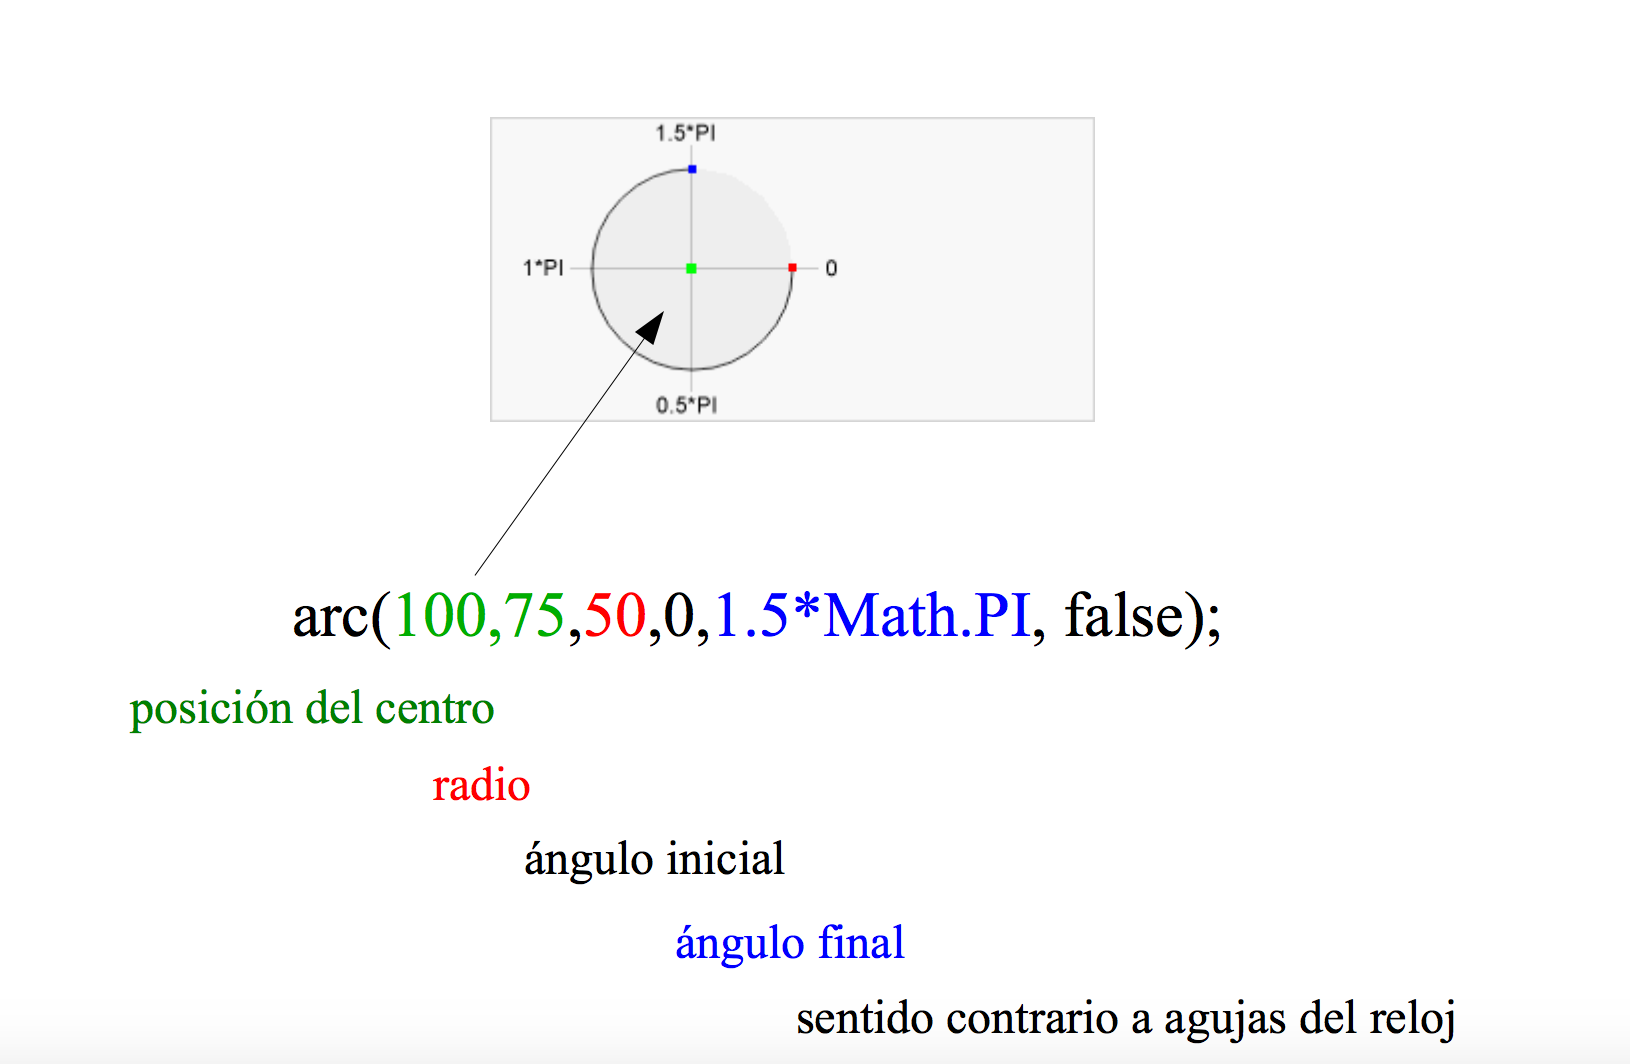
\includegraphics[trim=0cm 7cm 0cm 0cm, clip=true, width=0.75\textwidth]{img/arkuak}};
\end{tikzpicture}
\caption{Canvas osagaian arkuak margotzeko arc() funtzioa erabiliko dugu.}
\label{fig:canvasarkua}
\end{figure}

\begin{lstlisting}[language=HTML5, caption={Arku bat margotzeko kodea. Hemen eskuragarri: \href{https://codesandbox.io/s/canvas-arkua-75d7q}{https://codesandbox.io/s/canvas-arkua-75d7q}.}, label={lst:arkua}]
<!doctype html>
<html>
<head>
   <title>Canvas adibidea</title>
</head>
<body>
    <canvas id="oihala" width="150" height="150"></canvas>

<script>
var oihala = document.getElementById("oihala");
var ctx = oihala.getContext("2d");

ctx.arc(100,75,50,0,1.5*Math.PI, false);
ctx.stroke();

</script>
</body>
</html>
\end{lstlisting}

 
\section{Irudiak margotzen}
Irudi-fitxategiak ere canvas-en txerta ditzakegu. Oso funtzionalitate interesgarria du, jokoak HTML5en programatu nahi baditugu, adibidez. Honi esker, jokalaria (edo arerioak, edo ingurunea) ez dugu zertan lerroz lerro margotu, baizik eta jada existitzen diren sprite-ak (irudi-fitxategiak) canvas-en kargatu eta horiek mugituko ditugu (animazioak lortuz).

Hasteko, irudi bat canvas-en margotzeko, \hl{drawImage()}\index{drawImage()} metodoa erabiliko dugu. Metodo hori gainkargatuta dago. Ikus ditzagun adibide batzuk.

Lehenengo adibidean, UEUren ikurra kargatu eta canvas-en margotuko dugu.

\begin{lstlisting}[language=JavaScript, caption={UEUren logoa canvas-en margotuko dugu. Kodea hemen eskuragarri: \href{https://codesandbox.io/s/canvas-irudia-kk55q}{https://codesandbox.io/s/canvas-irudia-kk55q}.}, label={lst:canvas-ueu}]
<canvas id="oihala" width="120" height="110"></canvas>
<script>
 var oihala = document.getElementById("oihala");
 var context = oihala.getContext("2d");
 var logo = new Image();
 logo.src = "irudiak/ueu.png";
 
 // irudia memorian kargatzen denean oihalan idatziko dugu (ez lehenago)
 logo.onload = function() {
    context.drawImage(logo, 0, 0);
 };
</script>
\end{lstlisting}


\section{drawImage() metodoaren parametroak}
        \hl{drawImage()} metodoa gainkargatuta dago, alegia, posible da metodo horri deitzea 3, 5 edo 9 parametrorekin. Parametro kopuruaren arabera gauza bat edo bestea egingo du. Adibidez, 3 parametrorekin, zer margotu nahi dugun eta non (x,y) zehaztuko dugu. Bost parametro hartzen baditu, lehenengoa margotu nahi dugun irudiaren erreferentzia izango da (adibidean, \textit{logo} izeneko aldagaian kargatu duguna). Jarraian, x,y posizioa canvas-en. Adibidean, goi-ezkerreko pixelaren posizioa (0,0) izango da. Ondoren (eta adibidean agertzen ez direnak, hautazkoak baitira), canvas-en margotuko dugun irudiaren tamaina (zabalera, altuera). Ez badugu ezer zehazten, jatorrizko irudiaren tamaina eta canvas-en margotzen denaren tamaina berdinak izango dira. Interesgarriak dira azken bi parametro horiek animazio sinpleak lortzeko (irudia handituz edo txikituz). Bederatzi parametroren kasuan, lehenengo parametroa margotu nahi dugun irudiaren izena izango da. Jarraian dauden hurrengo 4 parametroek jatorrizko irudiaren zer zati (x, y, zabalera, altuera) hartu nahi dugun adierazten dute, eta, hurrengo laurek, canvas-en zer posiziotan eta zer tamainatan margotu nahi dugun zehazten dute.


\hlc[lightgray]{drawImage()} metodoaren 3 forma posibleen (3, 5 eta 9 parametrorekin) egindako adibide baten kodea hemen aurkituko dugu: \href{https://codesandbox.io/s/canvas-buster-ycmzu}{https://codesandbox.io/s/canvas-buster-ycmzu} (ikus \ref{fig:canvasbuster}. irudia).
Adibidean agertzen den testua, \hlc[lightgray]{fillText()}\index{fillText()} metodoa erabiliz margotu dugu. Zehazki:

\begin{lstlisting}[language=JavaScript,numbers=none]
// zer letra mota eta tamaina nahi dugun
        context.font = "20px Arial"; 
// idatzi nahi dugun testua eta non (canvas-eko posizioa)
        context.fillText("nahi duzun testua", 10, 150); 
\end{lstlisting}
        
\begin{figure}[ht]
	\centering
\begin{tikzpicture}
\node[anchor=south west,inner sep=0] (image) at (0,0)
   {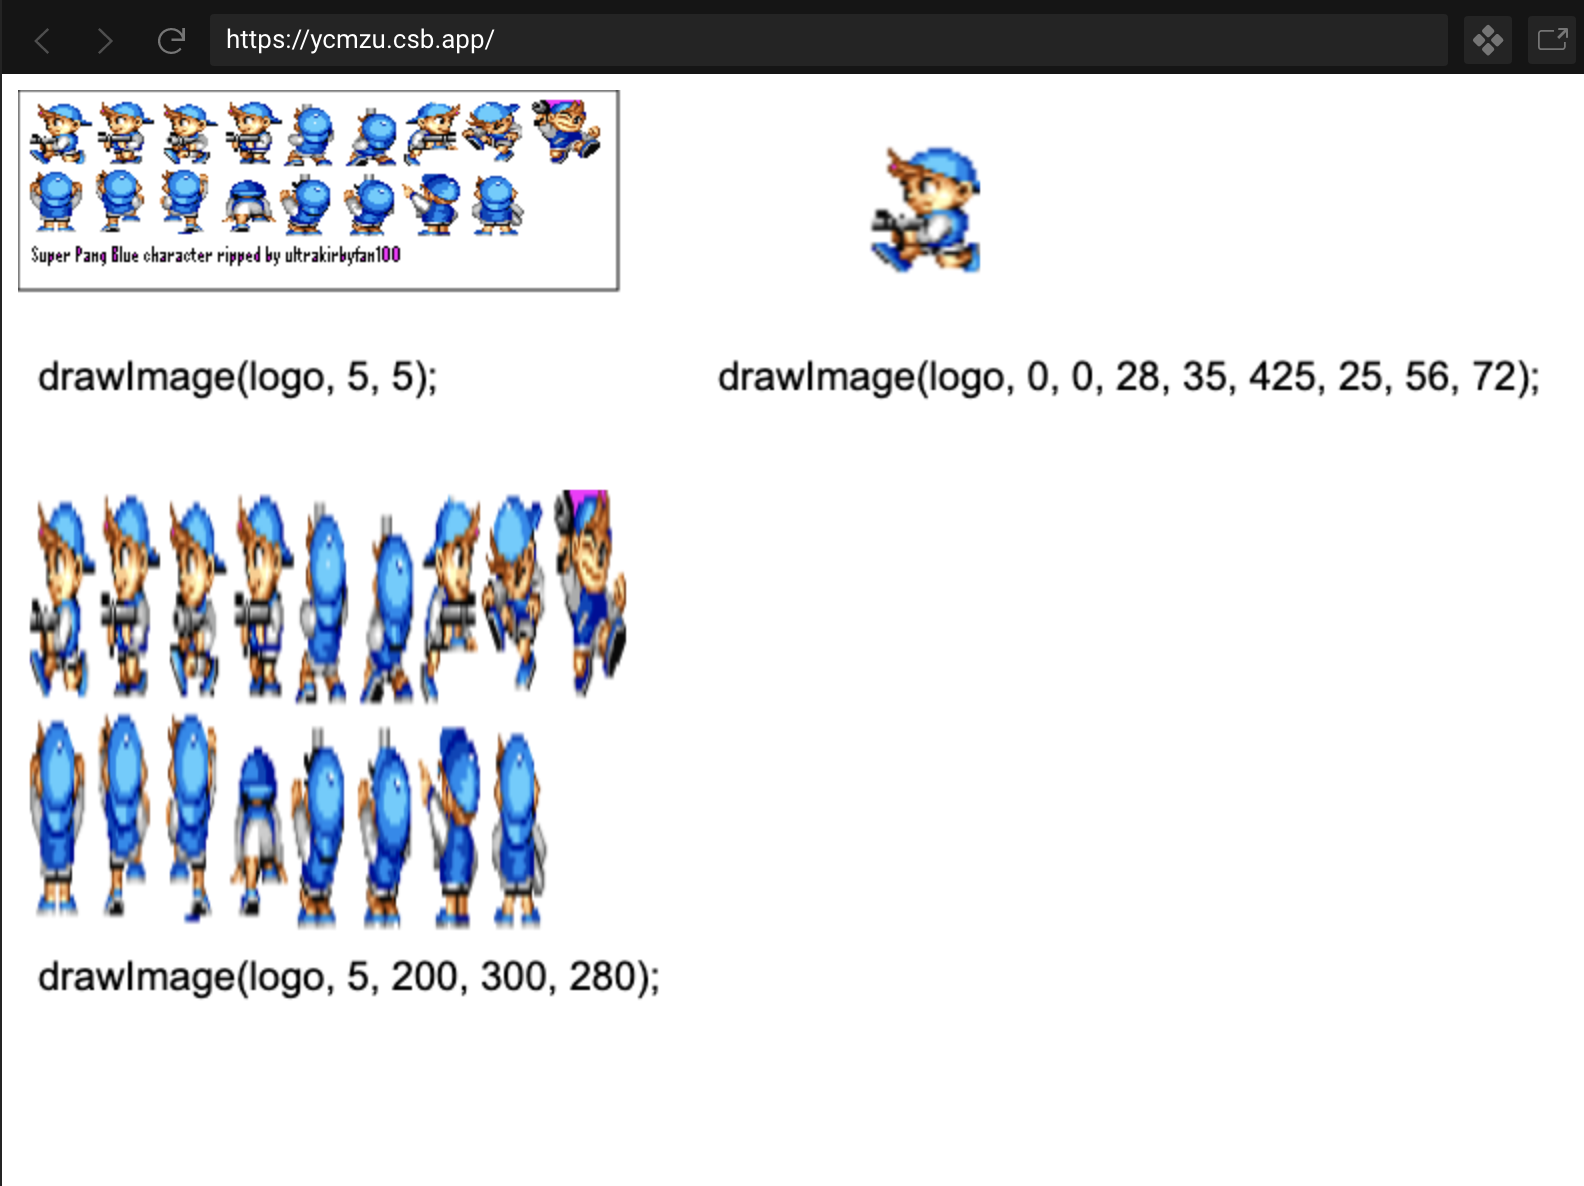
\includegraphics[trim=0cm 0cm 0cm 0cm, clip=true, width=0.75\textwidth]{img/canvasbuster}};
\end{tikzpicture}
\caption{Canvas osagaian irudiak margotzeko drawImage metodoa erabiliko dugu. Adibide honetan irudi bera agertzen da, baina drawImage erabiliz, irudiaren zati bat margotu dezakegu, aukeran zoom eginez, edo irudi osoa, berriro ere, aukeran zoom eginez. }
\label{fig:canvasbuster}
\end{figure}



% \begin{figure}[ht]
% 	\centering
% \begin{tikzpicture}
% \node[anchor=south west,inner sep=0] (image) at (0,0)
%    {
\includegraphics[trim=0cm 0cm 0cm 0cm, clip=true, width=0.75\textwidth]{img/drawimage}};
% \end{tikzpicture}
% \caption{Canvas osagaian irudiak margotzeko drawImage metodoa erabiliko dugu}
% \label{fig:drawimage}
% \end{figure}

\section{Ariketak}

Ariketa hauetan (\href{https://ikasten.io/html5/ariketak/08_gaia.pdf}{https://ikasten.io/html5/ariketak/08\_gaia.pdf}) sprite orri bat memorian kargatzen (ikus \ref{fig:canvasbuster}. irudia) ikasiko dugu. Baita sprite orri batetik irudi zehatzak ateratzen eta horiek canvas-en margotzen animazioak lortzeko. Zehazki,  Buster izeneko pertsonaiaren animazioa lortu nahi dugu.
\begin{enumerate}
    \item Hemengo helbidean \href{https://codesandbox.io/s/canvas-animazioa-8p7kx}{https://codesandbox.io/s/canvas-animazioa-8p7kx}) Buster-en irudi-orritik
(sprite orritik) lau posizio dinamikoki hartzeko kodea aurkituko duzu.

\begin{figure}[ht]
	\centering
\begin{tikzpicture}
\node[anchor=south west,inner sep=0] (image) at (0,0)
   {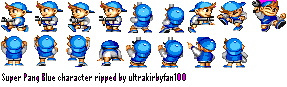
\includegraphics[trim=0cm 0cm 0cm 0cm, clip=true, width=0.75\textwidth]{img/canvas/player.png}};
\end{tikzpicture}
\caption{Buster pertsonaiaren zenbait animazio.}
\label{fig:playerbuster}
\end{figure}

Molda ezazu kodea setTimeInterval() metodoaren bidez Buster-en 4 posizio horiek leku berean,
amaigabeko bukle —begizta— batean, bata bestearen atzetik, 150 milisegundoan behin margotzeko,
animazioaren efektua lortuz. Dena ondo eginez gero, Buster ibiltzen ari dela emango du.

\item Aurreko ariketa moldatu Buster mugi dadin, pantaila eskuinetik hasita ezkerrerantz, ezkerreko
pareta ukitu arte (puntu horretan gelditu egin behar da).

\end{enumerate}
%% 9. Audioa eta Bideoa
\chapter{Audioa eta bideoa}\index{<video>}
\index{<audio>}\index{HTMLMediaElement}

HTML5 estandarrak <video> eta <audio> etiketak sartu zituen, eta horiekin batera, JavaScript bidez audioa eta bideoa kontrolatzeko HTMLMediaElement APIa. Bideoarekin lan egiten hasiko gara, termino batzuk definituz, \textit{kontainer}, \textit{codec} eta formatuak, besteak beste. 


\begin{figure}[ht]
	\centering
\begin{tikzpicture}
\node[anchor=south west,inner sep=0] (image) at (0,0)
   {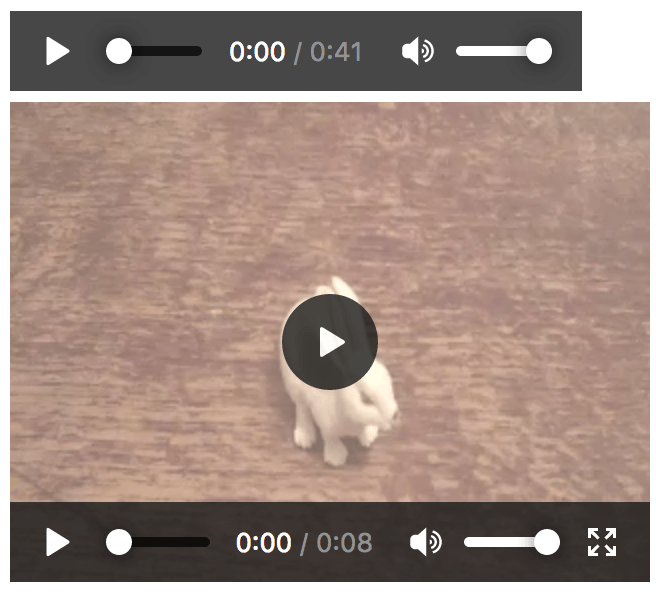
\includegraphics[trim=0cm 0cm 0cm 0cm, clip=true, width=0.75\textwidth]{img/native-controls-firefox.png}};
\end{tikzpicture}
\caption{Audio —goian— eta bideo —behean— kontrol-osagaiak.}
\label{fig:bideocontrols}
\end{figure}

\section{\textit{Kontainer} eta \textit{codec}-ak}\index{kontainer}\index{codec}
Bideo-fitxategi baten inguruan hitz egitean askotan entzun izan ditugu ``AVI fitxategi'' edo ``MP4 fitxategi'' hitzak. Baina AVI edo MP4 ez dira fitxategi mota bat, baizik eta kontainer motak. AVI MP4\index{MP4} edo WebM \index{WebM} kontainer batek, bere barnean, audio- eta bideo-kanalak gordetzen ditu, hainbat formatutan kodetuta egon daitezkeenak (\textit{codec} —kodek— ezberdinekin, Theora, H.264, VP9...).

\section{<video> etiketa}

Berez, bideo bat bistaratzeko etiketa sinple bat erabili ahal dugu:

\begin{verbatim}
    <video src="bideoa.webm"></video>
\end{verbatim}

Berriro, WebM kontainer mota bat da. Barruan duen bideoaren formatua (erabili den kodeka) zein den ez dakigu (bideoa jaitsi eta aztertu arte). HTML5 estandarrak \textit{<video>} etiketa eskaintzen badu ere, ez du zehazten bideoak erabili behar duen formatua... edo nabigatzaileak berak onartu behar dituen formatuak. Izan ere, hainbat aukera ditugu (\ref{fig:bideokodek} irudian adibide batzuk zehazten dira).

\begin{figure}[ht]
	\centering
\begin{tikzpicture}
\node[anchor=south west,inner sep=0] (image) at (0,0)
   {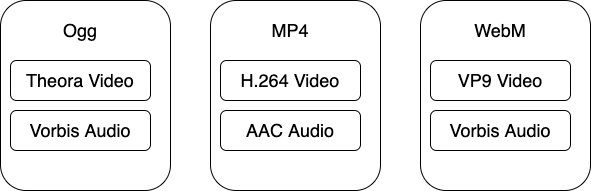
\includegraphics[trim=0cm 0cm 0cm 0cm, clip=true, width=0.75\textwidth]{img/bideoformatuak.png}};
\end{tikzpicture}
\caption{Bideo-kontainer eta \textit{codec}-en artean hainbat aukera ditugu.}
\label{fig:bideokodek}
\end{figure}

Nabigatzaile bakoitzak kodek zehatz bat onartzen duen edo ez jakiteko, Wikipediak eskaintzen duen \href{https://en.wikipedia.org/wiki/HTML5_video}{taulara joko dugu}\footnote{https://en.wikipedia.org/wiki/HTML5\_video} (ikus \ref{fig:bideokodekwikipedia}. irudia). Bertan kontainer eta kodeken bateragarritasuna nabigatzailearen arabera zehazten da.



\begin{figure}[ht]
	\centering
\begin{tikzpicture}
\node[anchor=south west,inner sep=0] (image) at (0,0)
   {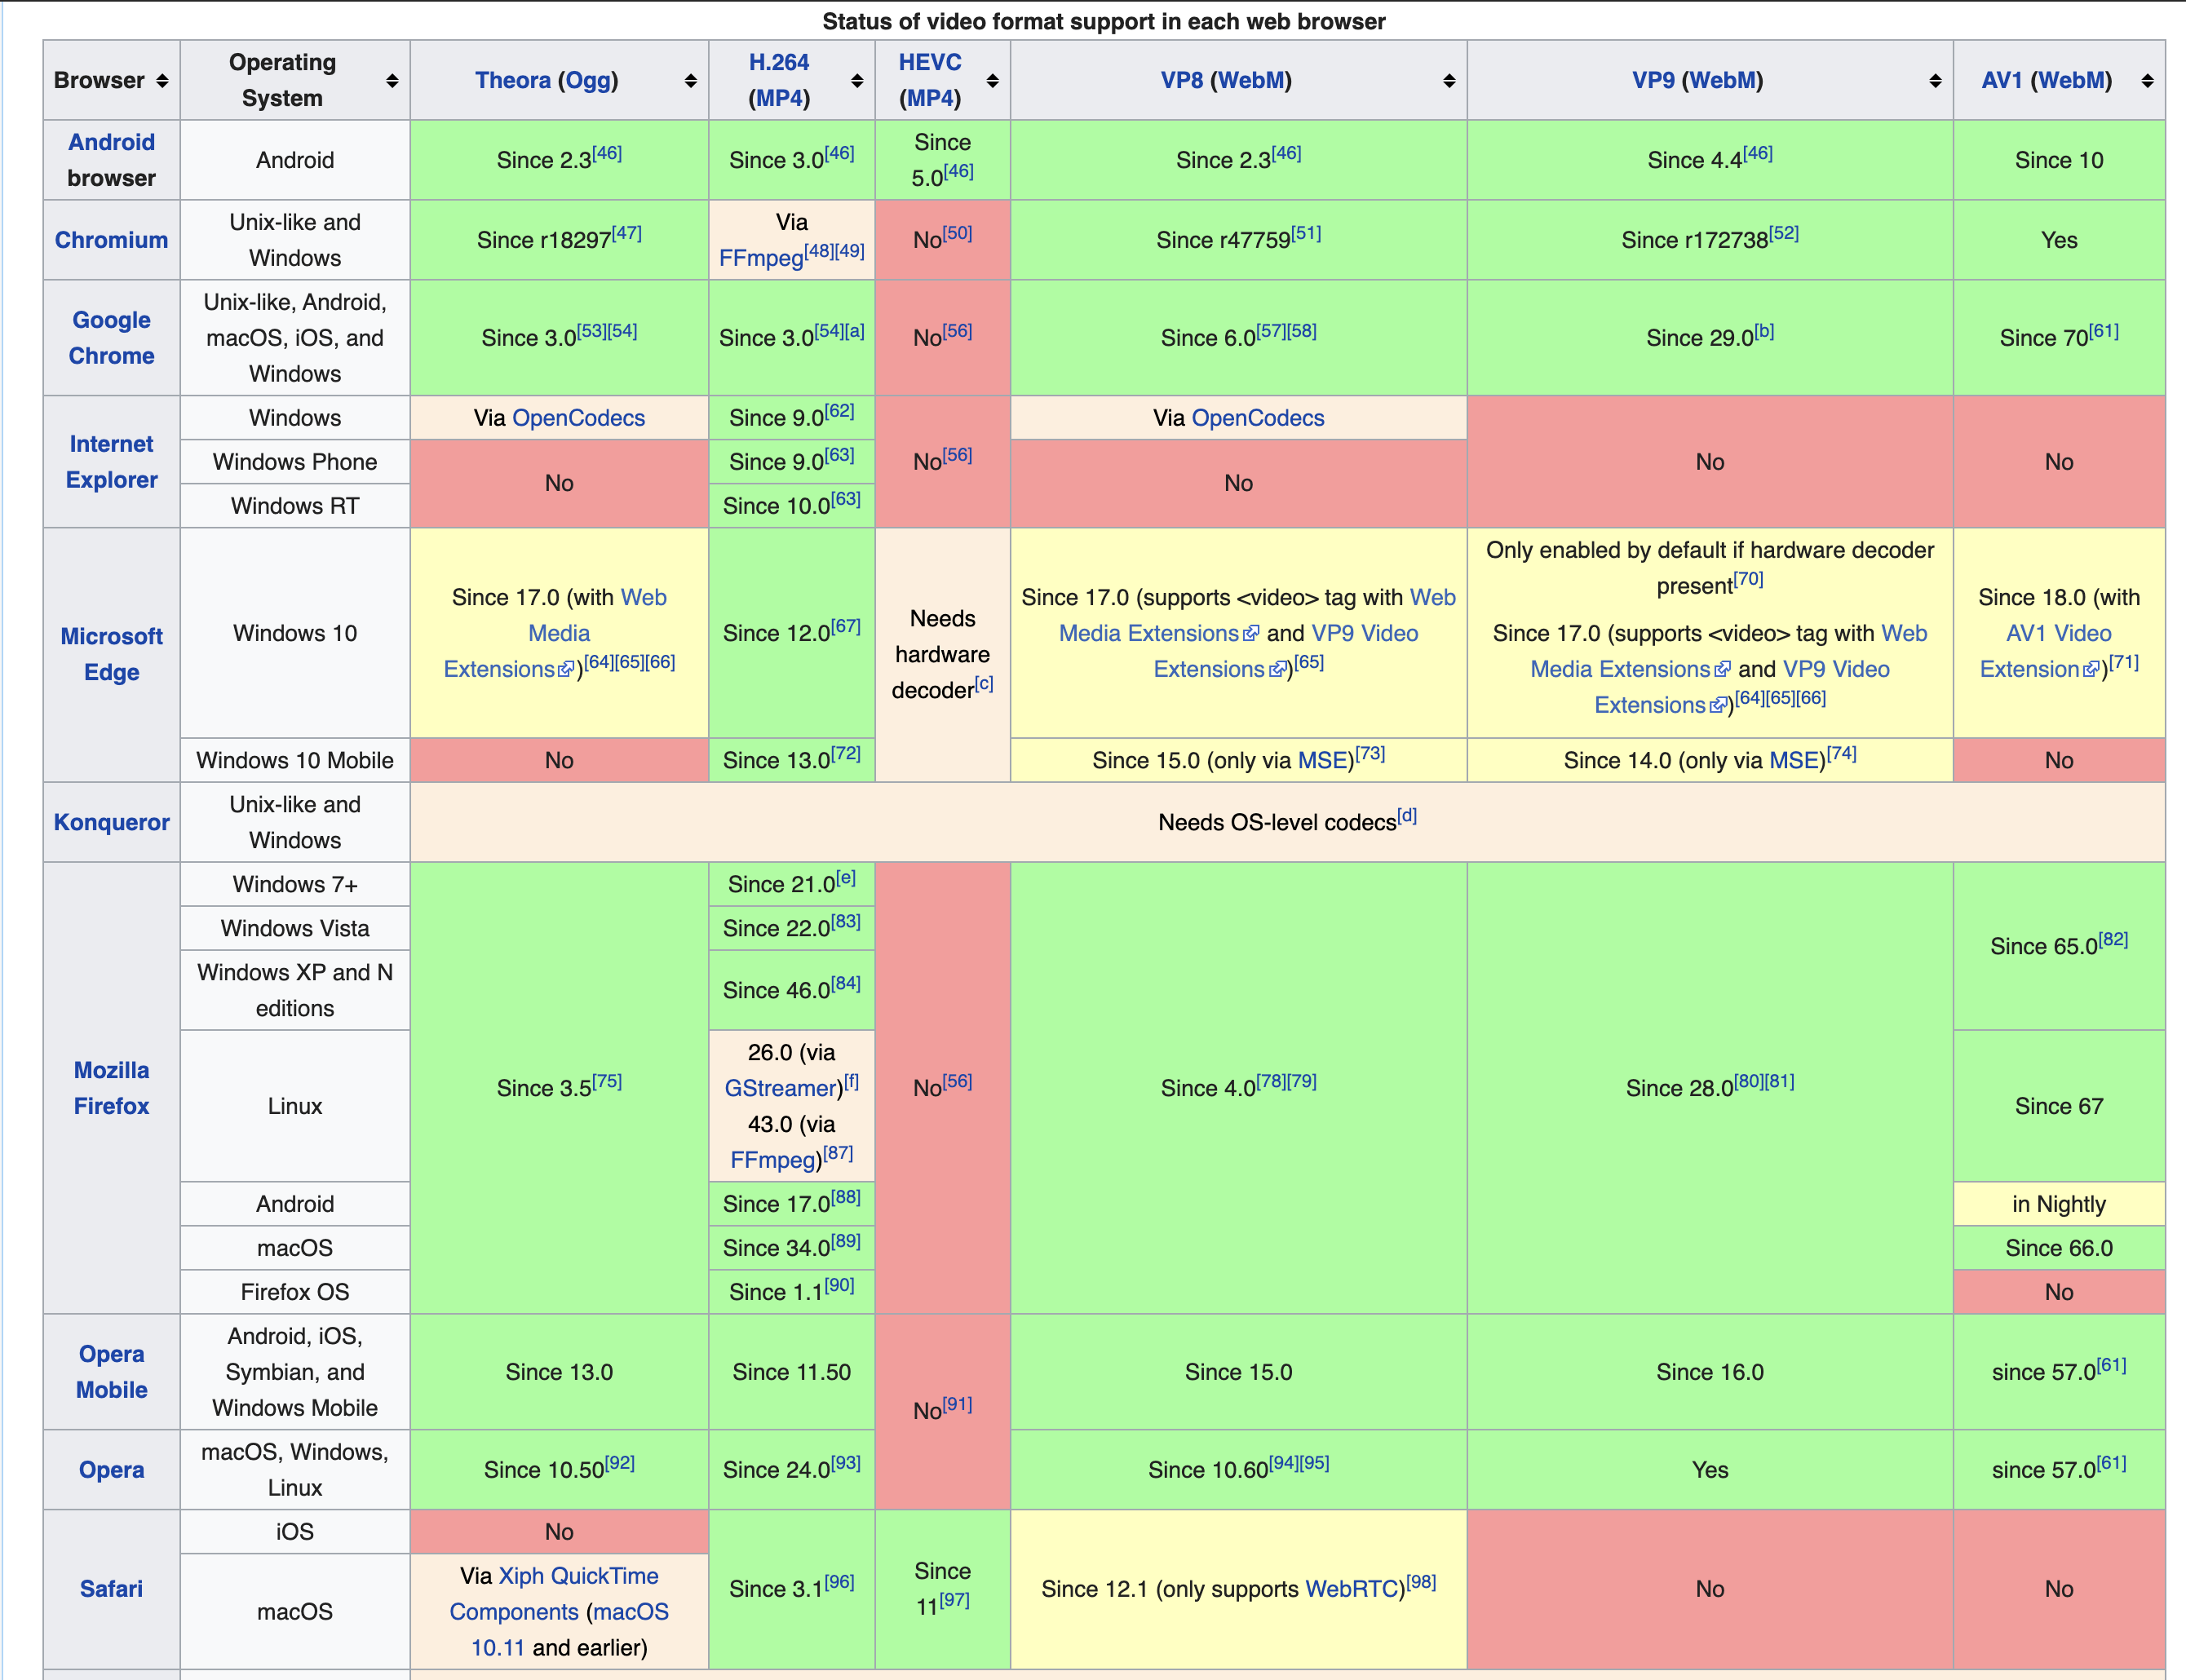
\includegraphics[trim=0cm 0cm 0cm 0cm, clip=true, width=0.75\textwidth]{img/kodekwikipedia.png}};
\end{tikzpicture}
\caption{Wikipediak badu orri bat nabigatzaileen arteko bideo-kodek eta kontainerren bateragarritasuna neurtzeko.}
\label{fig:bideokodekwikipedia}
\end{figure}


Hori guztia kontuan hartuta, ulertzekoa da <video> etiketaren erabilera aurkeztu dugun adibidea baino konplexuagoa izatea. Hurrengo listatuan <video> etiketaren erabileraren adibide zehatza ikus dezakegu:

\begin{lstlisting}[language=JavaScript,label={lst:bideoadibidea}]
<video width="320" height="240" controls>
 <source src="clip.mp4" type="video/mp4; codecs=avc1,mp4a">
 <source src="clip.webm" type="video/webm; codecs=vp8,vorbis">
 <source src="clip.ogv" type="video/ogg; codecs=theora,vorbis">
</video>
\end{lstlisting}

Bertan 320 x 240 tamainako bideo bat bistaratu nahi dugula zehaztu dugu. Bideoarekin batera, \textit{controls} atributuarekin, \textit{Play}, \textit{Pause}, \textit{FastForward} eta \textit{Rewind} egiteko aukera izan nahi dugula esaten ari gara.\index{<video> controls}

Horrez gain, \hl{type=video/mp4} atributuarekin, MP4 kontainerra hobesten dugula esaten ari gara, barruan avc1 bideo-kodeka eta mp4 audio-kodeka izango dituena (\hl{codecs=avc1,mp4a}). Hori ezinezkoa balitz (nabigatzaileak onartuko ez balu), orduan WebM kontainerra aukeratuko genuke, vp8 \index{VP8} bideo-kodek eta vorbis\index{Vorbis} audioarekin. Eta hori ere ezinezkoa balitz, orduan Ogg \index{OGG} kontainerra izango litzateke gure aukera, \textit{theora video} eta \textit{vorbis} audioarekin.

\textit{Controls} izeneko atributua ez da erabil dezakegun bakarra. Badugu autoplay\index{autoplay}, loop\index{loop}, preload\index{preload} eta poster\index{poster} izenekoak ere.

\begin{itemize}
    \item \textit{autoplay}: bideoa kargatu bezain pronto martxan jarri nahi dugula zehazten du.
    \item \textit{loop}: bideoa amaitzean berriro hasieratik automatikoki hasiko dela adierazteko.
    \item \textit{preload}: \hl{preload=auto} edo \hl{preload=metadata} izan daiteke atributu honen balioa. \textit{Auto}-ren kasuan, nabigatzaileari bideoa ahal bezain pronto kargatzea (orria kargatzen den unean) gomendatzen diogu. Alegia, erabiltzaileak \textit{play} botoian sakatu baino lehen, automatikoki buffer batean bideoa kargatzea nahi dugula zehazten du. Horrela erabiltzaileak \textit{play} botoian sakatzean, bideoa berehala hasiko da bistaratzen, inolako etenik gabe. \textit{Metadata}-ren kasuan gauza bera, baina bideo osoa aurrekargatu beharrean, bideoaren metadatuak (luzera, \textit{track} kopurua, bideoaren lehenengo fotograma, poster gisa erabiltzeko...) aurrekargatuko dira
   \item \textit{poster}: bideoa hasi baino lehen pantailan bideoari dagokion irudi txiki bat agertuko da.
\end{itemize}

Bideo bat JS erabiliz kontrolatzeko API bat daukagu eskuragarri HTML5en. Metodo, atributu eta gertaera asko eskaintzen baditu ere, garrantzitsuenak \ref{tab:bideoAPI}. taulan aurki daitezke.

% Please add the following required packages to your document preamble:
% \usepackage{booktabs}
\begin{table}[]
\begin{tabular}{@{}lllll@{}}
\toprule
\multicolumn{2}{c}{\textbf{Atributuak}} & \multicolumn{1}{c}{\textbf{Metodoak}} & \multicolumn{2}{c}{\textbf{Gertaerak}} \\ \midrule
width            & currentTime          & play()   \index{play()}                             & progress            & timeupdate       \\
height           & paused               & pause()   \index{pause()}                            & loadeddata          & volumechange     \\
loop             & duration             & load() \index{load()}                               & error               & ended            \\
muted            & readyState           & canPlayType()   \index{canPlayType()}                       & loadedmetadata      & play            \\
ended            & seeking              &                                       & pause               & abort            \\
error            & volume               &                                       & waiting             &                  \\ \bottomrule
\end{tabular}
\caption{Bideoak JavaScript-ez kontrola ditzakegu, hainbat metodo, atributu eta gertaeraren bidez.}
\label{tab:bideoAPI}
\end{table}

Bideoen inguruko APIa hobeto ulertzeko adibide pare bat ekarriko ditugu hona. Lehenengoak hiru bideo kargatzen ditu array batean eta, APIa erabiliz, bata bestearen ondoren joko ditu. 

\begin{lstlisting}[language=JavaScript]
let position = -1;
let playlist;
let bideo;
window.onload = function() {
	playlist = ["video/bat.mp4","video/bi.mp4", "video/hiru.mp4"];
	bideo = document.getElementById("video");
	bideo.addEventListener("ended", hurrengoBideoa);
        hurrengoBideoa();
}

function hurrengoBideoa(){
     position++;
     if (position >=  playlist.length) position = 0;
     bideo.src = playlist[position];
     bideo.load();
     bideo.play();
}
\end{lstlisting}


Bigarren adibidean gauza bera egiten dugu, baina bideoa martxan jarri baino lehen bideoaren kontainerra nabigatzaileak onartzen duen edo ez begiratuko dugu. 

\begin{lstlisting}[language=JavaScript]

window.onload = function() {
// ...
	playlist = ["video/bat","video/bi", "video/hiru"];
// ...
}
function hurrengoBideoa(){
// ...
     bideo.src = playlist[position] + getFormatExtension();
// ...
}
function getFormatExtension() {
    if (bideo.canPlayType("video/mp4") != "") {
    	    return ".mp4";
    } else if (bideo.canPlayType("video/ogg") != "") {
        return ".ogv";
    } else if (bideo.canPlayType("video/webm") != "") {
        return ".webm";
    }
}
\end{lstlisting}


 \begin{alertinfo}{canPlayType() metodoaren balio posibleak}
        Bideoa baten \textit{canPlayType()}\index{canPlayType()} metodoak parametro bat hartzen du, bideoaren kontainer mota (adibidez "video/webm", edo "video/mp4") eta hiru balio posible itzultzen ditu: kate hutsa (""), "maybe" edo "probably". Kate hutsaren kasuan, nabigatzaileak kontainer mota hori ez duela onartzen esan nahi du. \textit{maybe} kasuan, agian bistaratu dezakeela eta \textit{probably} ia ziur onartzen duela. Nabigatzaileak ezin du erabat ziurtatu jo ahal duen edo ez, kontainer baten barruan kodek ezberdinak egon daitezkeelako.
    \end{alertinfo}

\section{Audio-etiketa}\index{<audio>}

Audioaren eta bideoaren etiketek oso antzera funtzionatzen dute. Ikus bestela honako HTML5 <audio> etiketaren adibidea:

\begin{lstlisting}[language=JavaScript]
<audio controls>
<source src="horse.ogg" type="audio/ogg">
<source src="horse.mp3" type="audio/mpeg">
Zure nabigatzaileak ez du audio etiketa onartzen.
</audio>
\end{lstlisting}

Ogg motako kontainerra ez bada onartzen, orduan MP3 kontainer mota duen audioarekin saiatuko gara. Horrekin ere ezin badu nabigatzaileak, orduan errore-mezu bat emango dugu. Ohart zaitez \textit{controls} atributua ere erabiltzen ari garela, \textit{<video>} etiketan egin genuen bezala.

Nabigatzaileek audio-formatuekin duten bateragarritasun-maila jakin ahal izateko badugu Wikipedian orri berezi bat ere\footnote{\href{http://en.wikipedia.org/wiki/HTML5\_Audio}{http://en.wikipedia.org/wiki/HTML5\_Audio}}.

\section{Ariketak}

Ariketa multzo honetan canvas eta <video> etiketak uztartuko ditugu, adibidez \ref{fig:bideoariketa}. irudian dagoen ariketa egiteko. 

\begin{figure}[ht]
	\centering
\begin{tikzpicture}
\node[anchor=south west,inner sep=0] (image) at (0,0)
   {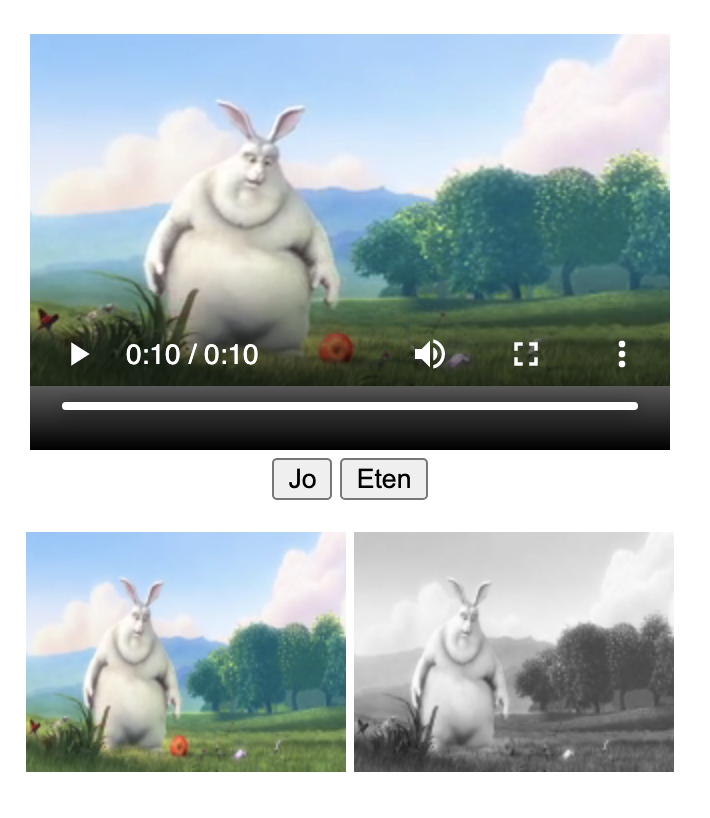
\includegraphics[trim=0cm 0cm 0cm 0cm, clip=true, width=0.75\textwidth]{img/azala.png}};
\end{tikzpicture}
\caption{Bideo batetik fotogramak atera daitezke eta canvas batean utzi baino lehen itxuraz aldatu. Adibidez, irudia zuri-beltz bihurtzeko.}
\label{fig:bideoariketa}
\end{figure}

Hemengo kode-adibideari jarraituz
\href{https://codesandbox.io/s/bideo-ariketa-1-bh3cg}{https://codesandbox.io/s/bideo-ariketa-1-bh3cg}:

\begin{enumerate}
    \item  Controls atributua ezabatu <video> etiketatik. Jarraian 3 botoi prestatu bideoaren azpian agertzeko: Jo, Eten, Kaptura.

\begin{itemize}
    \item Jo botoian sakatzean, bideoa martxan jarriko da.
     \item  Eten botoian sakatzean, bideoa eten egingo da. Berriro martxan jartzeko, Jo botoian sakatu.
     \item Kaptura botoian sakatzean, bideoaren uneko fotogramaren kaptura egingo da. Kaptura
     <canvas> etiketan bistaratu behar da, dimentsioak aldatuz —txikiagoa ikusi behar da bideoa baino, zuk aukeratu tamaina—. Adibide gisa, ikus \ref{fig:bideoariketa2}. irudia.
     
\begin{figure}[ht]
\centering
\begin{tikzpicture}
\node[anchor=south west,inner sep=0] (image) at (0,0)
   {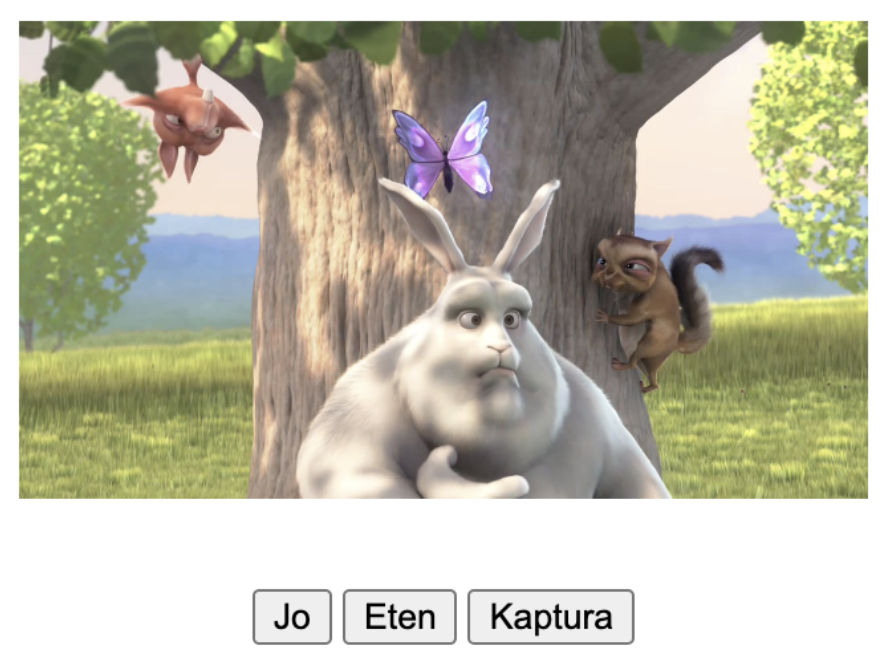
\includegraphics[trim=0cm 0cm 0cm 0cm, clip=true, width=0.75\textwidth]{img/audiobideo/joetenkaptura.png}};
\end{tikzpicture}
\caption{Kaptura botoian sakatzean uneko fotogramaren kaptura egin behar da eta tamaina txikian margotu, irudian bezala.}
\label{fig:bideoariketa2}
\end{figure}
     
Argibidea:\textit{ drawImage()} metodoak lehenengo parametroan bideo baten erreferentzia onartzen du. 
\end{itemize}

Ariketaren soluzioa begiratu gabe egiten saia zaitez, baina argibideren bat behar baduzu, hona hemen ariketaren soluzioa:\newline \href{https://codesandbox.io/s/bideoariketak-soluzioa-i3kp8}{ https://codesandbox.io/s/bideoariketak-soluzioa-i3kp8}

\item Aurreko ariketa moldatu bideoaren kapturak automatikoki egin daitezen, alegia \textit{canvas} osagaian bideoaren fotogramak agertuko dira bideoa martxan dagoen bitartean, automatikoki.

Honako lerro hau lagungarria egingo zaizu:

\begin{lstlisting}[language=JavaScript,numbers=none]
bideoa.addEventListener("play", function () { .... zure kodea ... }
\end{lstlisting}

Bideoa amaitzen denean edo bideoa etetean (``pause'' egitean), \textit{canvas} osagaian fotogramak kopiatzeari utzi.

Beste lerro hau ere lagungarria egingo zaizu:

\begin{lstlisting}[language=JavaScript,numbers=none]
bideoa.addEventListener("pause", function () { ... zure kodea hemen ...}
\end{lstlisting}

Ariketaren soluzioa begiratu gabe egiten saia zaitez, baina argibideren bat behar baduzu, hona hemen: \href{https://codesandbox.io/s/bideosoluzioa2-jiqyn}{https://codesandbox.io/s/bideosoluzioa2-jiqyn}.


\item Hurrengo ariketan <video> eta <canvas> etiketak uztartuko ditugu. Helburua \ref{fig:bideoariketa}. irudian dugun aplikazio lortzea da. Goiko aldean bideo bat dugu. Haren azpian bi canvas txiki. Ezkerrekoan orain arte egin duguna.
Eskuinekoan zuri-beltzez margotuko dugun beste canvas bat. Prozesua honakoa da:

\begin{itemize}
    \item Bideotik frame bat atera eta ezkerreko canvas osagaian (\textit{buffer} deritzona) utzi:

buffer.drawImage(bideoa, 0, 0, 160, 120);

Jarraian, bufferetik frame baten informazioa erauzi, array gisa:

\begin{lstlisting}[language=JavaScript,numbers=none]
let frame = buffer.getImageData(0, 0, 320, 120);
\end{lstlisting}

frame arrayak \ref{fig:bideoariketa2}. irudiko itxura izango du:

\begin{figure}[ht]
\centering
\begin{tikzpicture}
\node[anchor=south west,inner sep=0] (image) at (0,0)
   {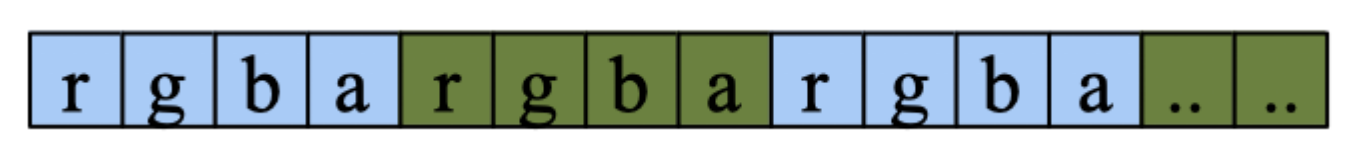
\includegraphics[trim=0cm 0cm 0cm 0cm, clip=true, width=0.75\textwidth]{img/audiobideo/rgba.png}};
\end{tikzpicture}
\caption{R = Red-Gorria, G = Green-Berdea, B = Blue-Urdina, A = Alpha-Gardentasuna.}
\label{fig:bideoariketa2}
\end{figure}
     

Alegia, pixel bakoitzak 4 balio izango ditu: R (\textit{red} edo kolore gorria), G (\textit{green} edo berdea), B (\textit{blue}
edo urdina), A (\textit{alpha} edo gardentasun-maila). Adibidez, pixel bat guztiz gorria eta  erdi gardena izango bagenu, orduan haren balioa (255, 0, 0, 100) izango litzateke. 

Zenbat pixel ditugun jakiteko, zatiketa sinple bat egin dezakegu:

\begin{lstlisting}[language=JavaScript,numbers=none]
let length = frame.data.length / 4;
\end{lstlisting}

Ondoren, pixel bakoitzeko, haren posizioa eta (r,g,b,a) balioak aterako ditugu eta horiekin
zuri-beltzez() izeneko funtzio bati deituko diogu, kolorez dagoen pixel bat zuri-beltz bihurtzeko:

\begin{lstlisting}[language=JavaScript,numbers=none]
for (let i = 0; i < length; i++) {
 let r = frame.data[i * 4 + 0];
 let g = frame.data[i * 4 + 1];
 let b = frame.data[i * 4 + 2];
 zuri-beltzez(i, r, g, b, frame.data);
 }
\end{lstlisting} 
 
 zuri-beltzez() funtzioa erraza da, kolore-osagai bakoitzaren balioak batu eta batezbestekoa lortuko
du hasieran (kolore grisa lortzeko). Ondoren pixel horri kolore grisa esleitzen dio:


\begin{lstlisting}[language=JavaScript,numbers=none]
function zuri-beltzez(pos, r, g, b, data) {
 var grisa = (r + g + b) / 3;
 data[pos * 4 + 0] = grisa;
 data[pos * 4 + 1] = grisa;
 data[pos * 4 + 2] = grisa;
}
\end{lstlisting}

Egitea falta zaigun bakarra zuri-beltzez lortu dugun frame arraya canvas-en margotzea da:
\begin{lstlisting}[numbers=none]
zuri-beltza.putImageData(frame, 0, 0);
\end{lstlisting}

Ariketaren soluzioa begiratu gabe egiten saia zaitez, baina argibideren bat behar baduzu, hona hemen: \href{https://juananpe.github.io/txuribeltz/}{https://juananpe.github.io/txuribeltz/}.

\item Audio-ariketa batekin jarraituko dugu. Hiru fitxategiz osatutako array bat dugularik:
\textit{[\textquotesingle{}audio1.mp3\textquotesingle{}, \textquotesingle{}audio2.mp3\textquotesingle{}, \textquotesingle{}audio3.mp3\textquotesingle{}]}, programa ezazu script bat hiru audio horiek jotzeko, bata bestearen atzetik. Bukatzean, lehenengoarekin jarraitu, amaigabeko begizta batean.
\end{itemize}

\end{enumerate}
%% 10. Biltegiratze lokala
\chapter{Biltegiratze lokala, localStorage APIa}
\index{localStorage}\index{stateless}

HTTP protokoloak ez du memoriarik. Eskaera baten eta ondorengoen artean protokoloak ez du ezer gogoratzen, hau da, \textit{stateless} protokoloa dela esaten dugu. Adibide batekin aztertuko dugu hau. Demagun hiru web orri ditugula (ikus \ref{fig:localstorage1}. irudia):

\begin{figure}[ht]
	\centering
\begin{tikzpicture}
\node[anchor=south west,inner sep=0] (image) at (0,0)
   {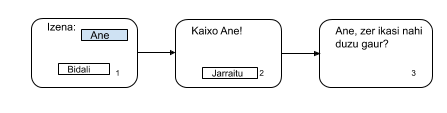
\includegraphics[trim=0cm 0cm 0cm 0cm, clip=true, width=.75\textwidth]{img/localstorage/localstorage1.png}};
\end{tikzpicture}
\caption{HTTP protokoloak ez du memoriarik. Formulario batek jasotzen duen informazioa bistaratzeko ez dago arazorik, baina 3. pantaila batera informazio hori bidaltzeko bai, ordea.}
\label{fig:localstorage1}
\end{figure}


Lehenengo orrian, erabiltzaileari izena eskatzen zaio. Kasu honetan ``Ane'' idatzi, \hl{Bidali} botoian sakatu eta bigarren orrira goaz. Bertan zerbitzariak ``Kaixo Ane!'' idatzi behar du eta jarraitzeko botoi bat eskaini. Hau lortzeko ez dugu arazorik, ``Ane'' izena parametro gisa baitoa formularioan. Baina bigarren orritik hirugarren orrirako jauzian, nola bidali ``Ane'' izena? Aukera bat izan daiteke \mbox{\textit{hidden}} motako eremu batean bidaltzea. Baina badago beste aukera bat sartu ditugun datuak HTTP zerbitzariari gogorarazteko: cookieak \index{cookie} erabiltzea. Honela funtzionatuko du (ikus \ref{fig:localstorage2} irudia):

\begin{figure}[ht]
	\centering
\begin{tikzpicture}
\node[anchor=south west,inner sep=0] (image) at (0,0)
   {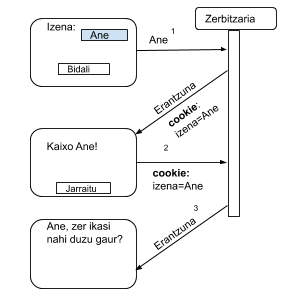
\includegraphics[trim=0cm 0cm 0cm 0cm, clip=true, width=.35\textwidth]{img/localstorage/localstorage2.png}};
\end{tikzpicture}
\caption{HTTP protokoloan egoera mantentzeko cookieak erabiltzen ohi dira.}
\label{fig:localstorage2}
\end{figure}


Erabiltzaileak Ane izena sartu eta Bidali botoian sakatu ondoren, zerbitzariak ``Ane'' parametroa jaso eta erabiltzaileari hurrengo orria bidaltzen dio, cookie batekin batera (cookiearen balioa izena=Ane delarik). Erabiltzailearen nabigatzaileak, hemendik aurrera, zerbitzari horri edozein gauza eskatzearekin batera beti bidaliko dio jaso duen cookiea, lekuko bat izango balitz bezala. Bigarren pausoan zerbitzariak cookiea jaso eta izena=Ane ikusita badaki zeinek bidali dion. Gauzak horrela, azken (hirugarren) orrialdea prestatu eta nabigatzaileari bidaliko dio, 
``Ane, zer ikasi nahi duzu gaur'' testuarekin batera. Landu dugun adibide honen inplementazioarekin praktikatzeko, hemengo\footnote{https://gist.github.com/juananpe/824b1d9ad2141d5c64bc8693492863f9} kodea erabili (martxan ikusi nahiko bazenu, Heroku aplikazio honetan \footnote{https://mighty-anchorage-92406.herokuapp.com/} argitaratu da).

Beraz, cookieek informazioa gordetzeko balio dute, eta, horrekin batera, HTTP protokoloari egoera gogoratzeko bide bat emango diogu. % Cookieek saioak gordetzeko ere balioko dute baina hori beste gai batean jorratuko da. 

\begin{alertinfo}{Informazio pribatua eta cookieak}
Adi! Ez gorde informazio pribatua cookie baten barruan (adibidez, ez gorde inoiz pasahitzak cookie baten barruan). Horren ordez, cookiean identifikatzaile bat gorde dezakegu eta zerbitzariaren lana izango da cookie horren identifikatzaileari edukia esleitzea eta gordetzea. Horrela, informazio pribatua zerbitzarian gordeko da beti, eta ez bezeroan. 
\end{alertinfo}

Cookie baten tamaina maximoa 4 KB da, beraz biltegiratze lokala lortzeko ez du askotarako ematen. Baina HTML5ek beste API bat eskaintzen du datuak bezeroan gorde eta kudeatu ahal izateko, Web Storage API \index{Web Storage API} delakoa.

\section{Web Storage APIa}

API honek \textit{izena=balioa} formatuari jarraitzen dioten balioen biltegiratze lokala (\textit{localStorage} \index{localStorage} delakoa) ahalbidetzen du. Domeinu bakoitzeko 5-10 MB gorde ditzake nabigatzailean bertan. Cookieekin ez bezala, behar direnean erabiltzen dira (gogoratu cookieen kasuan nabigatzaileak beti bidali behar zituela zerbitzarira).

\textit{LocalStorage} biltegian idazteko \textit{setItem} \index{setItem} metodoa erabiliko dugu:

\begin{lstlisting}[language=javascript,numbers=none]
localStorage.setItem("gakoa", balioa);
\end{lstlisting}

Eta balio bat irakurtzeko, \textit{getItem}:
\index{getItem}
\begin{lstlisting}[language=javascript,numbers=none]
let balioa = localStorage.getItem("gakoak");
\end{lstlisting}
 
LocalStorage array bat izango balitz bezala ere trata daiteke, bai datuak irakurtzeko:

\begin{lstlisting}[language=javascript,numbers=none]
let balioa  = localStorage["gakoa"];
\end{lstlisting}

nola gordetzeko:

\begin{lstlisting}[language=javascript,numbers=none]
localStorage["gakoa"] = balioa;
\end{lstlisting}

Balio bat localStorage-tik ezabatzeko, \textit{removeItem}  \index{removeItem} erabiliko dugu:

\begin{lstlisting}[language=javascript,numbers=none]
localStorage.removeItem("gakoa");
\end{lstlisting}


Posible da, halaber, localStorage biltegian dauden aldagai guztiak ezabatzea, \textit{clear} metodoarekin \index{clear}:

\begin{lstlisting}[language=javascript,numbers=none]
localStorage.clear();
\end{lstlisting}

\textit{length} atributua eta \textit{key()} metodoaren laguntzaz, localStorage biltegiko balioak zeharka ditzakegu \index{length}\index{key}:

\begin{lstlisting}[language=javascript,numbers=none]
for (let i=localStorage.length; i >= 0; i--){
    let gakoa = localStorage.key(i);
    console.log( localStorage.get(gakoa) );
}
\end{lstlisting}

\subsection{Nola aztertu localStorage biltegian dagoen edukia}

Firefox-en \textit{Biltegiratzea} izeneko erlaitzean, \textit{Biltegiratze lokala} atalean aurkituko dugu localStorage biltegia, domeinuka antolatuta. Adibidez, \ref{fig:localstorage3} irudian, berria.eus webgunean sartzean gordetzen den informazioa ikus daiteke.

\begin{figure}[ht]
	\centering
\begin{tikzpicture}
\node[anchor=south west,inner sep=0] (image) at (0,0)
   {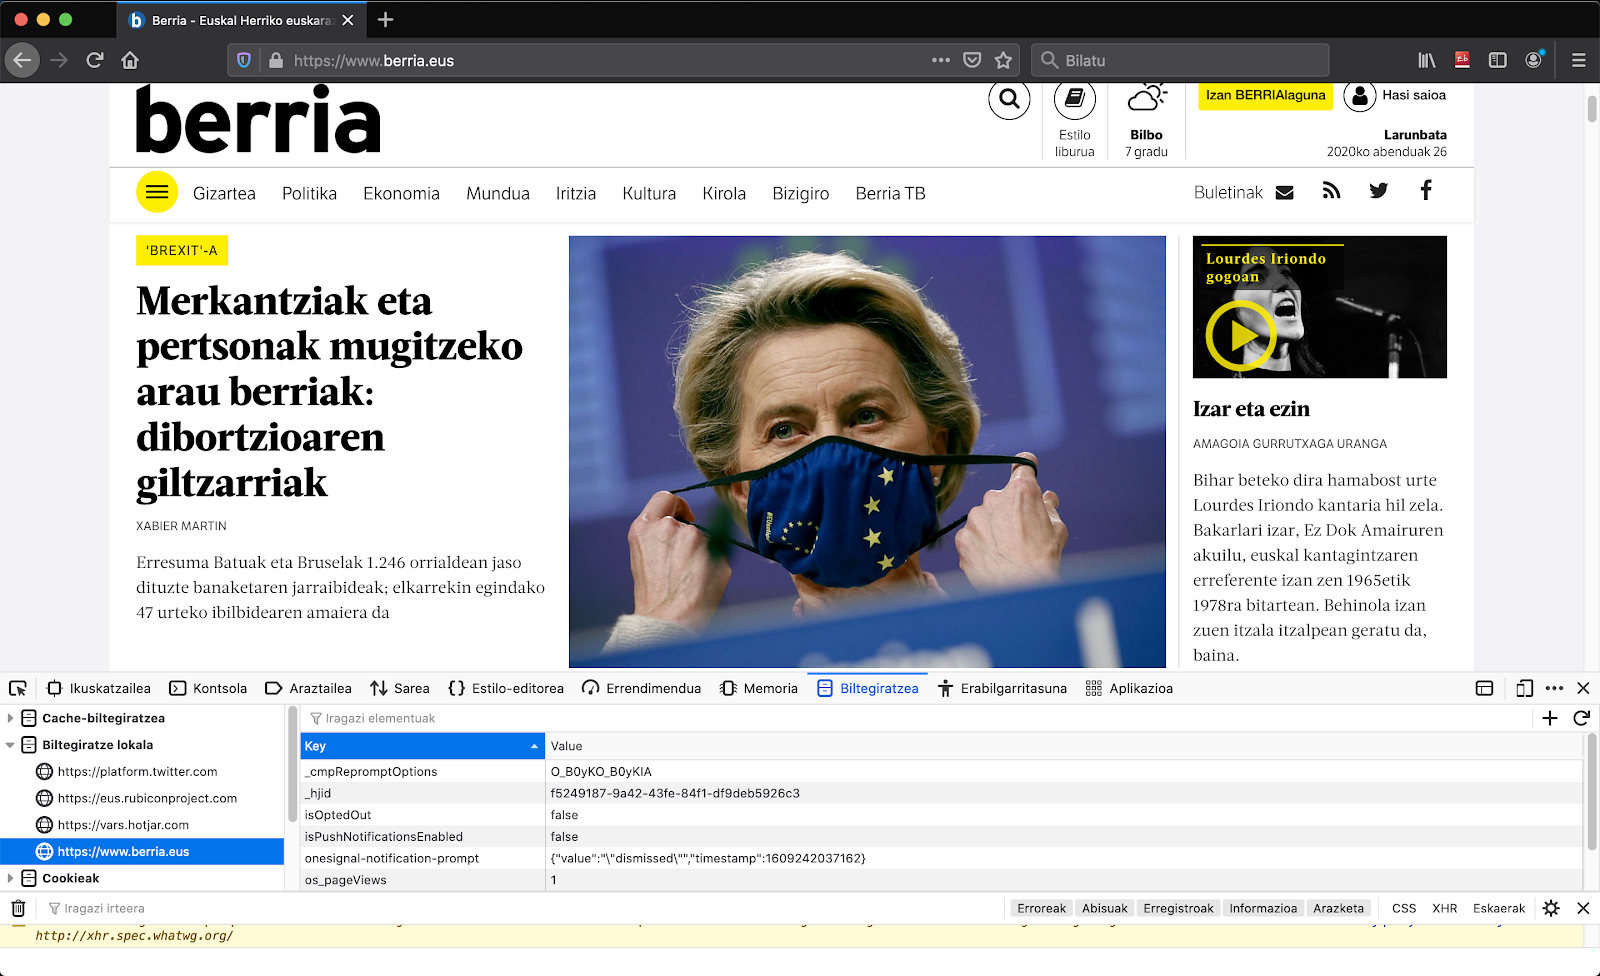
\includegraphics[trim=0cm 0cm 0cm 0cm, clip=true, width=.70\textwidth]{img/localstorage/localstorage3.png}};
\end{tikzpicture}
\caption{Berriak localStorage erabiltzen du hainbat informazio nabigatzailean bertan gordetzeko, besteak beste erabiltzailearen baimena (\textit{push})\index{push} jakinarazpenak jaso nahi dituen edo ez zehazteko.}
\label{fig:localstorage3}
\end{figure}

Kontsolan \textit{localStorage.clear()} \index{clear} metodoari deitzean, bertan zeuden datu guztiak ezabatu ahalko ditugu.

% \begin{figure}[ht]
% 	\centering
% \begin{tikzpicture}
% \node[anchor=south west,inner sep=0] (image) at (0,0)
%    {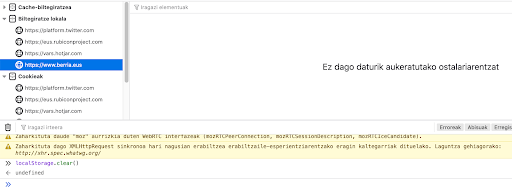
\includegraphics[trim=0cm 0cm 0cm 0cm, clip=true, width=.5\textwidth]{img/localstorage/localstorage4.png}};
% \end{tikzpicture}
% \caption{localstorage4}
% \label{fig:localstorage4}
% \end{figure}

LocalStorage biltegia hutsik dagoelarik, berriro kargatzen badugu berria.eus webgunea, Berriak (push) jakinarazpenak jaso nahi ditugun galdetuko digu (\ref{fig:localstorage5} irudia). 


\begin{figure}[ht]
	\centering
\begin{tikzpicture}
\node[anchor=south west,inner sep=0] (image) at (0,0)
   {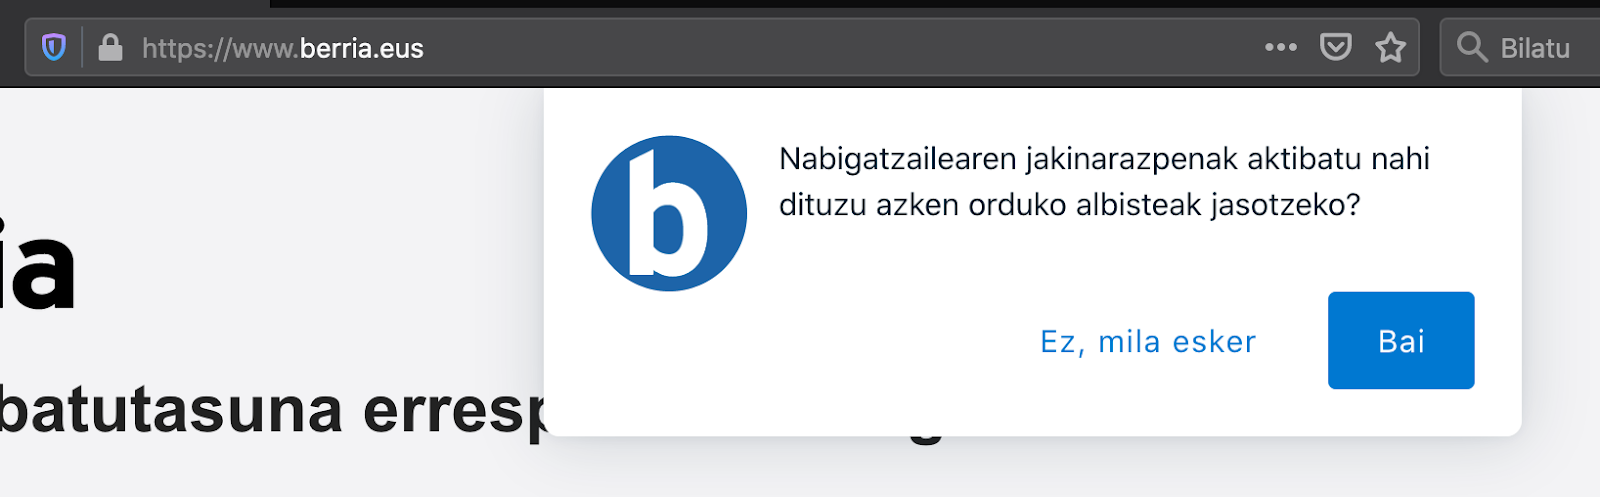
\includegraphics[trim=0cm 0cm 0cm 0cm, clip=true, width=.5\textwidth]{img/localstorage/localstorage5.png}};
\end{tikzpicture}
\caption{Berriak push jakinarazpenak jaso nahi ditugun edo ez galdetuko digu lehendabiziko bisitan. Erabiltzailearen erantzuna localStorage biltegian gordetzen da (horrela ez zaio berriro ere galdetuko hurrengo bisitan).}
\label{fig:localstorage5}
\end{figure}

% Dirudienez localStorage-n gordetzen du jakinarazpenak jaso nahi ditugun edo ez, isPushNotificationsEnabled aldagaian:
% 
% \begin{figure}[ht]
% 	\centering
% \begin{tikzpicture}
% \node[anchor=south west,inner sep=0] (image) at (0,0)
%    {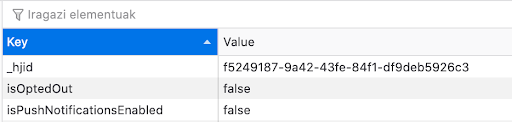
\includegraphics[trim=0cm 0cm 0cm 0cm, clip=true, width=.5\textwidth]{img/localstorage/localstorage6.png}};
% \end{tikzpicture}
% \caption{localstorage6}
% \label{fig:localstorage6}
% \end{figure}

\newpage
\section{Ariketak}

OpenLibrary APIa erabil dezakegu liburu baten datuak lortzeko bere ISBNa pasatuz. Adibidez:
 
 
\begin{lstlisting}[language=javascript,numbers=none]
 fetch("https://openlibrary.org/api/books? bibkeys=ISBN:9781491906187&
 jscmd=details&format=json").then( r=> r.json()).then( r => console.log (r['ISBN:9781491906187'].details))
\end{lstlisting}
   
    

% \begin{figure}[ht]
% 	\centering
% \begin{tikzpicture}
% \node[anchor=south west,inner sep=0] (image) at (0,0)
%    {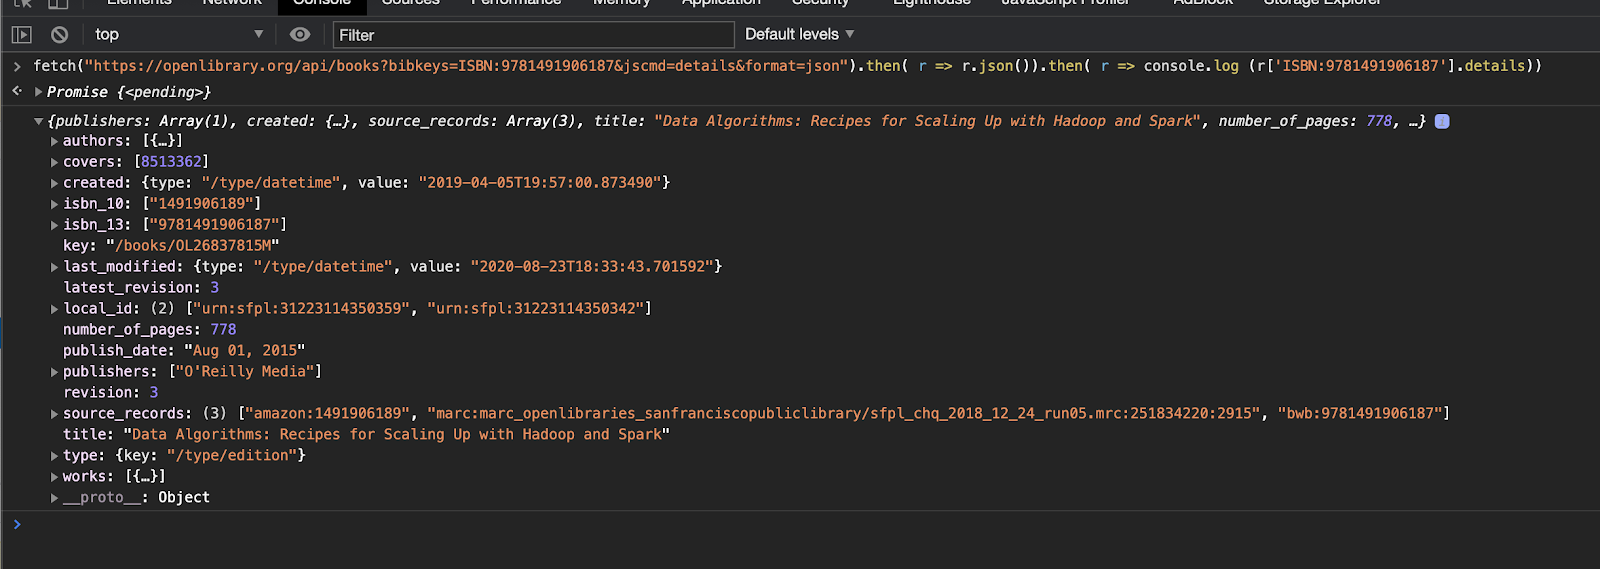
\includegraphics[trim=0cm 0cm 0cm 0cm, clip=true, width=.75\textwidth]{img/localstorage/localstorage7.png}};
% \end{tikzpicture}
% \caption{OpenLibrary APIa erabiliz liburu baten metadatuak jaso ditzakegu. Horiek localStorage biltegian gordetzea da ariketa honen helburua.}
% \label{fig:localstorage7}
% \end{figure}
%

 OpenLibrary APIa erabiliz, egin ezazu programa bat ISBN array honetan dauden liburu guztien datuak localStorage biltegian gordetzeko:
 
\begin{lstlisting}[language=javascript,numbers=none] 
 ['ISBN:9781491906187', 'ISBN:9781491920497', 'ISBN:1491910399',
     'ISBN:1491946008', 'ISBN:1491978236', 'ISBN:9781491906187']
 \end{lstlisting}
 
 Bukatzean, dena ondo egin badugu, kode hau exekutatzean:
 
 \begin{lstlisting}[language=javascript,numbers=none]
 let liburua = localStorage.getItem( 'ISBN:9781491906187');
  console.log( liburua.title ); 
 \end{lstlisting}
 
 
 Emaitza hau jaso beharko genuke:
 "Data Algorithms: Recipes for Scaling Up with Hadoop and Spark".
 
 \textbf{Soluzioa}:
 \href{https://github.com/juananpe/express/blob/master/public/js/module.mjs}{https://github.com/juananpe/express/blob/master/public/js/module.mjs}
 
 

%% 11. Geokokapena
\chapter{Geokokapen APIa}

Geokokapen APIak erabiltzailearen kokapen zehatza aurkitzeko metodoak eskaintzen ditu. API hau bereziki interesgarria da HTML5 euskarria ematen duten gailu mugikorretan erabiltzeko. W3C erakundeak argitaratutako espezifikazioa bada ere, berez geokokapen APIa ez dago HTML5en espezifikazioaren barruan.
API honen bidez, munduko puntu baten geokokapena lortu ahalko dugu, adibidez: Bilbo, latitudea: 43° 15' iparra, longitudea: 2° 55' mendebaldea.
Ikus dezagun API honen erabileraren adibide bat. Gure helburua uneko geokokapena lortzea izango da.

\begin{figure}[ht]
	\centering
\begin{tikzpicture}
\node[anchor=south west,inner sep=0] (image) at (0,0)
   {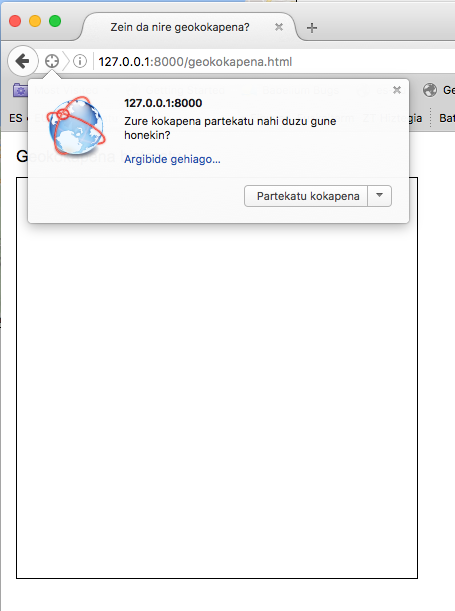
\includegraphics[trim=0cm 0cm 0cm 0cm, clip=true, width=0.5\textwidth]{img/geopermission}};
\end{tikzpicture}
\caption{Geokokapena lortzeko nabigatzaileak erabiltzaileari baimena eskatu behar dio (lehendabiziko aldia bada).}
\label{fig:kokapenabaimena}
\end{figure}

\begin{figure}[ht]
	\centering
\begin{tikzpicture}
\node[anchor=south west,inner sep=0] (image) at (0,0)
   {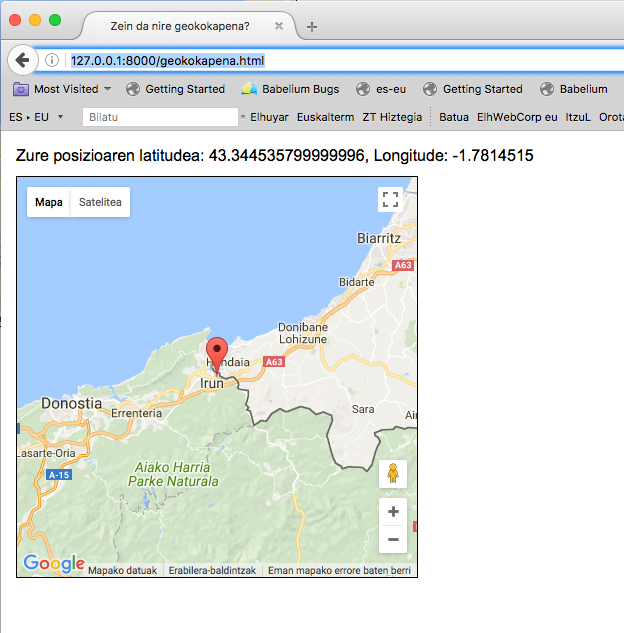
\includegraphics[trim=0cm 0cm 0cm 0cm, clip=true, width=0.5\textwidth]{img/geoapi}};
\end{tikzpicture}
\caption{Google Maps API eta geokokapen APIa erabiliz, uneko kokapena lortu eta mapa batean margotu dugu.}
\label{fig:kokapenagooglemaps}
\end{figure}

\begin{alertinfo}{HTTPS protokoloa erabili geokokapena partekatu ahal izateko}
       Segurtasuna dela eta, ezin da file:// protokoloa erabili geokokapena lortzeko. Alegia, HTTP zerbitzari bat beharko duzu gai honen inguruko ariketak egiteko. Askotan ikasleek file:// protokoloa erabiltzen dute beren probak egiteko. Orain arte horrela egiteak ez zuen inolako oztoporik sortzen, baina orain bai, ordea. Ez baduzu Apache (HTTP zerbitzari ezagunena) instalatu edo konfiguratu nahi, Python erabil dezakezu, modu errazean HTTP zerbitzari bat martxan jarri ahal izateko:

       \$ python -mSimpleHTTPServer 

Komando horrek Pythonek eskaintzen duen HTTP zerbitzari sinple bat martxan jarriko du, 8000 portuan entzunez, uneko karpetaren fitxategiak eskainiz. Orain, nabigatzailean, http://localhost:8000 edo http://127.0.0.1:8000 idatziz, HTTP protokoloa erabili ahalko duzu gai honen ariketak modu erraz batean probatu ahal izateko. Pribatutasuna dela eta, HTTPS da erabili beharreko protokoloa localhost domeinua ez badugu erabiltzen.
\end{alertinfo}

\section{Posizioa lortzen. getCurrentPosition metodoa}

\textit{getCurrentPosition()} \index{getCurrentPosition()} metodoaren sinadura hau da:

\begin{lstlisting}[numbers=none]
getCurrentPosition(callback, errorea, aukerak)   
\end{lstlisting}


Funtzio horri deitzean, nabigatzaileak egiaztatu beharko du ea erabiltzaileak posizioa ezagutzeko baimena eman duen edo ez. Baiezkoan, \textit{callback} funtzioari deituko dio. Ezezkoan, erabiltzaileari galdetu eta haren erantzunaren arabera \textit{callback} edo errore-funtzioari deituko dio (ikus \ref{fig:geolocationapi}. irudia). \textit{Aukerak} izeneko hautazko parametroaren bidez kokapenaren zehaztasun batzuk ezar daitezke.

\begin{lstlisting}[numbers=none,language=JavaScript]
// defektuzko balioak 
let aukerak = {
enableHighAccuracy: false, // zehaztasun maila altua nahi den edo ez
timeout: Infinity,  // asko jota zenbat denbora itxaron behar den geokokapena lortzen errorerik eman gabe
maximumAge: 0 // cachean dauden geokokapenen denbora maximoa berrerabiliak ahal izateko, milisegundutan. 0 = ez erabili cachea
}
\end{lstlisting}

Ikus dezagun adibide zehatz bat (inplementazioa \href{https://codesandbox.io/s/geokokapena-v9vbz?file=/index.html}{hemen\footnote{https://github.com/yuchenlin/rebiber}} proba dezakezu).

\begin{figure}[ht]
	\centering
\begin{tikzpicture}
\node[anchor=south west,inner sep=0] (image) at (0,0)
   {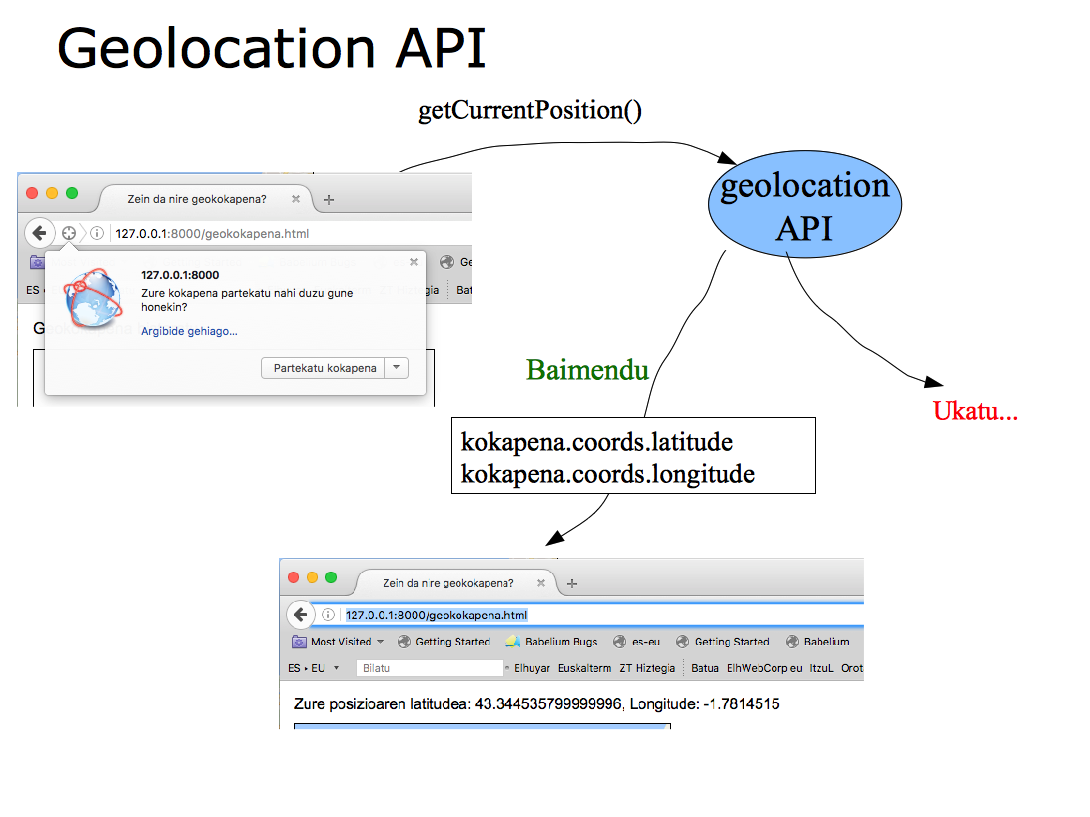
\includegraphics[trim=0cm 0cm 0cm 0cm, clip=true, width=0.5\textwidth]{img/geolocation_api_eu}};
\end{tikzpicture}
\caption{Kokapena: Nola funtzionatzen duen Geolocation \index{Geolocation API} APIak.}
\label{fig:geolocationapi}
\end{figure}

\begin{lstlisting}[language=JavaScript]
window.onload = lortuGeokokapena;

function lortuGeokokapena() {

// nabigatzaileak geolocation APIa inplementatzen du?
	if (navigator.geolocation) {

		navigator.geolocation.getCurrentPosition( bistaratuGeokokapena , bistaratuErrorea);
	}
	else {
		alert("Nabigatzaile honek ez du geokokapen APIa onartzen");
	}
}

function bistaratuGeokokapena(posizioa) {
	let latitude = posizioa.coords.latitude;
	let longitude = posizioa.coords.longitude;

	let div = document.getElementById("geokokapena");
	div.innerHTML = "Zure posizioaren latitudea: " + latitude + ", Longitude: " + longitude;

//	mapaBistaratu(posizioa.coords);

}

function bistaratuErrorea(error) {
	const errorTypes = {
		0: "Errore ezezagun",
		1: "Ez duzu kokapena lortzeko baimenik",
		2: "Kokapena ez dago eskuragarri",
		3: "Itxaron denbora agortu da"
	};
	let errorMessage = errorTypes[error.code];
	if (error.code == 0 || error.code == 2) {
		errorMessage = errorMessage + " " + error.message;
	}
	let div = document.getElementById("geokokapena");
	div.innerHTML = errorMessage;
}
\end{lstlisting}

\begin{alertinfo}{macOS sistema erabiltzen duzu?}
Adi! macOS sistema eragilean bazaude Security\&Privacy fitxan Chrome edo Firefox nabigatzaileei geokokapena lortzeko baimena eman beharko diezu Geolocation APIa erabili ahal izateko.
\end{alertinfo}

\section{Geokokapena Google Maps-en marrazten}
Aurreko kodean erabiltzailearen geokokapena lortu dugu, baina ez dugu mapa batean marraztu. Horretarako, Google Maps-eko APIaren laguntza beharko dugu. Ohart zaitez aurreko kodean 22. lerroa komentatuta dagoela (\textit{mapaBistaratu} metodoari deia). Lerro hori deskomentatu eta jarraian dugun \textit{mapaBistaratu} metodoa aztertu. 

\begin{lstlisting}[language=HTML5]
<head>
<script type="text/javascript" src="//maps.googleapis.com/maps/api/js?key=GAKOA"> </script>
</head>
<body>
<div id="kokapena">
Zure geokokapena hemen bistaratuko da.
</div>
<div id="mapa">
</div>

</body>
</html>
\end{lstlisting}

\begin{alertinfo}{Google Maps API key}
Adi! Google Maps-eko APIa erabiltzeko API gako bat eskatu beharko duzu hemen \href{https://developers.google.com/maps/documentation/javascript/get-api-key}{https://developers.google.com/maps/documentation/javascript/get-api-key}
\end{alertinfo}


\begin{lstlisting}[language=JavaScript]
let map; // aldagai globala

function mapaBistaratu(coords) {
let googleLatAndLong = new google.maps.LatLng(coords.latitude,coords.longitude);

const mapOptions = {
zoom: 10,
center: googleLatAndLong,
mapTypeId: google.maps.MapTypeId.ROADMAP
};

let mapDiv = document.getElementById("mapa");
map = new google.maps.Map(mapDiv, mapOptions);
}
\end{lstlisting}

Bi metodo erabiltzen ari gara hemen, 
\index{google.maps.LatLng}\textit{google.maps.LatLng} (mapan kokatu nahi dugun puntuaren latitudea eta longitudea parametro gisa espero dituena)  eta \textit{google.maps.Map}\index{google.maps.Map} eraikitzailea. Horrek bi parametro jasotzen ditu: \textit{div} etiketa baten erreferentzia (mapa zer geruzatan marraztu nahi dugun jakiteko) eta aukera-objektu bat, \textit{mapOptions}, zer motatako mapa eta zer zoomekin ikusi nahi dugun zehazteko.

Orain arte landutako adibidea \href{https://ikasten.io/html5/geokokapena.html}{https://ikasten.io/html5/geokokapena.html} webgunean aurki dezakezu.

\subsection{Markatzaileak}
Falta zaigun gauza bakarra markatzaile gorri bat jartzea da (\textit{marker} bat). Markatzaile horren gainean klik egitean, gure uneko kokapena agertuko da maparen gainean. Presta dezagun \hl{markatzaileaGehitu} izeneko funtzio bat. 

\begin{lstlisting}[language=JavaScript]
function markatzaileaGehitu(mapa, latlong, izenburua, edukia){
    let markerOptions = {
        position: latlong,
        map: mapa,
        title: izenburua,
        clickable: true
    };
    let marker = new google.maps.Marker(markerOptions);
    

    let infoWindowOptions = {
        content: edukia,
        position: latlong
    };
    let infoWindow = new google.maps.InfoWindow(infoWindowOptions);
    google.maps.event.addListener(marker, "click", function() {
        infoWindow.open(mapa);
    });
}
\end{lstlisting}

Orain \textit{mapaBistaratu()} funtziotik, \textit{markatzaileaGehitu} funtzioari deituko diogu:
\begin{lstlisting}[language=JavaScript]
let izenburua = "Zure kokapena";
let edukia = "Hemen zaude kokatua: " + coords.latitude + ", " + coords.longitude;
markatzaileaGehitu(map, googleLatAndLong, izenburua, edukia);
\end{lstlisting}

Markatzaileak erabiltzen dituen kodearen adibidea online ikusteko, jo ezazu honako helbide honetara: \newline
\href{https://ikasten.io/html5/markadorea.html}{https://ikasten.io/html5/markadorea.html}
\begin{figure}[ht]
	\centering
\begin{tikzpicture}
\node[anchor=south west,inner sep=0] (image) at (0,0)
   {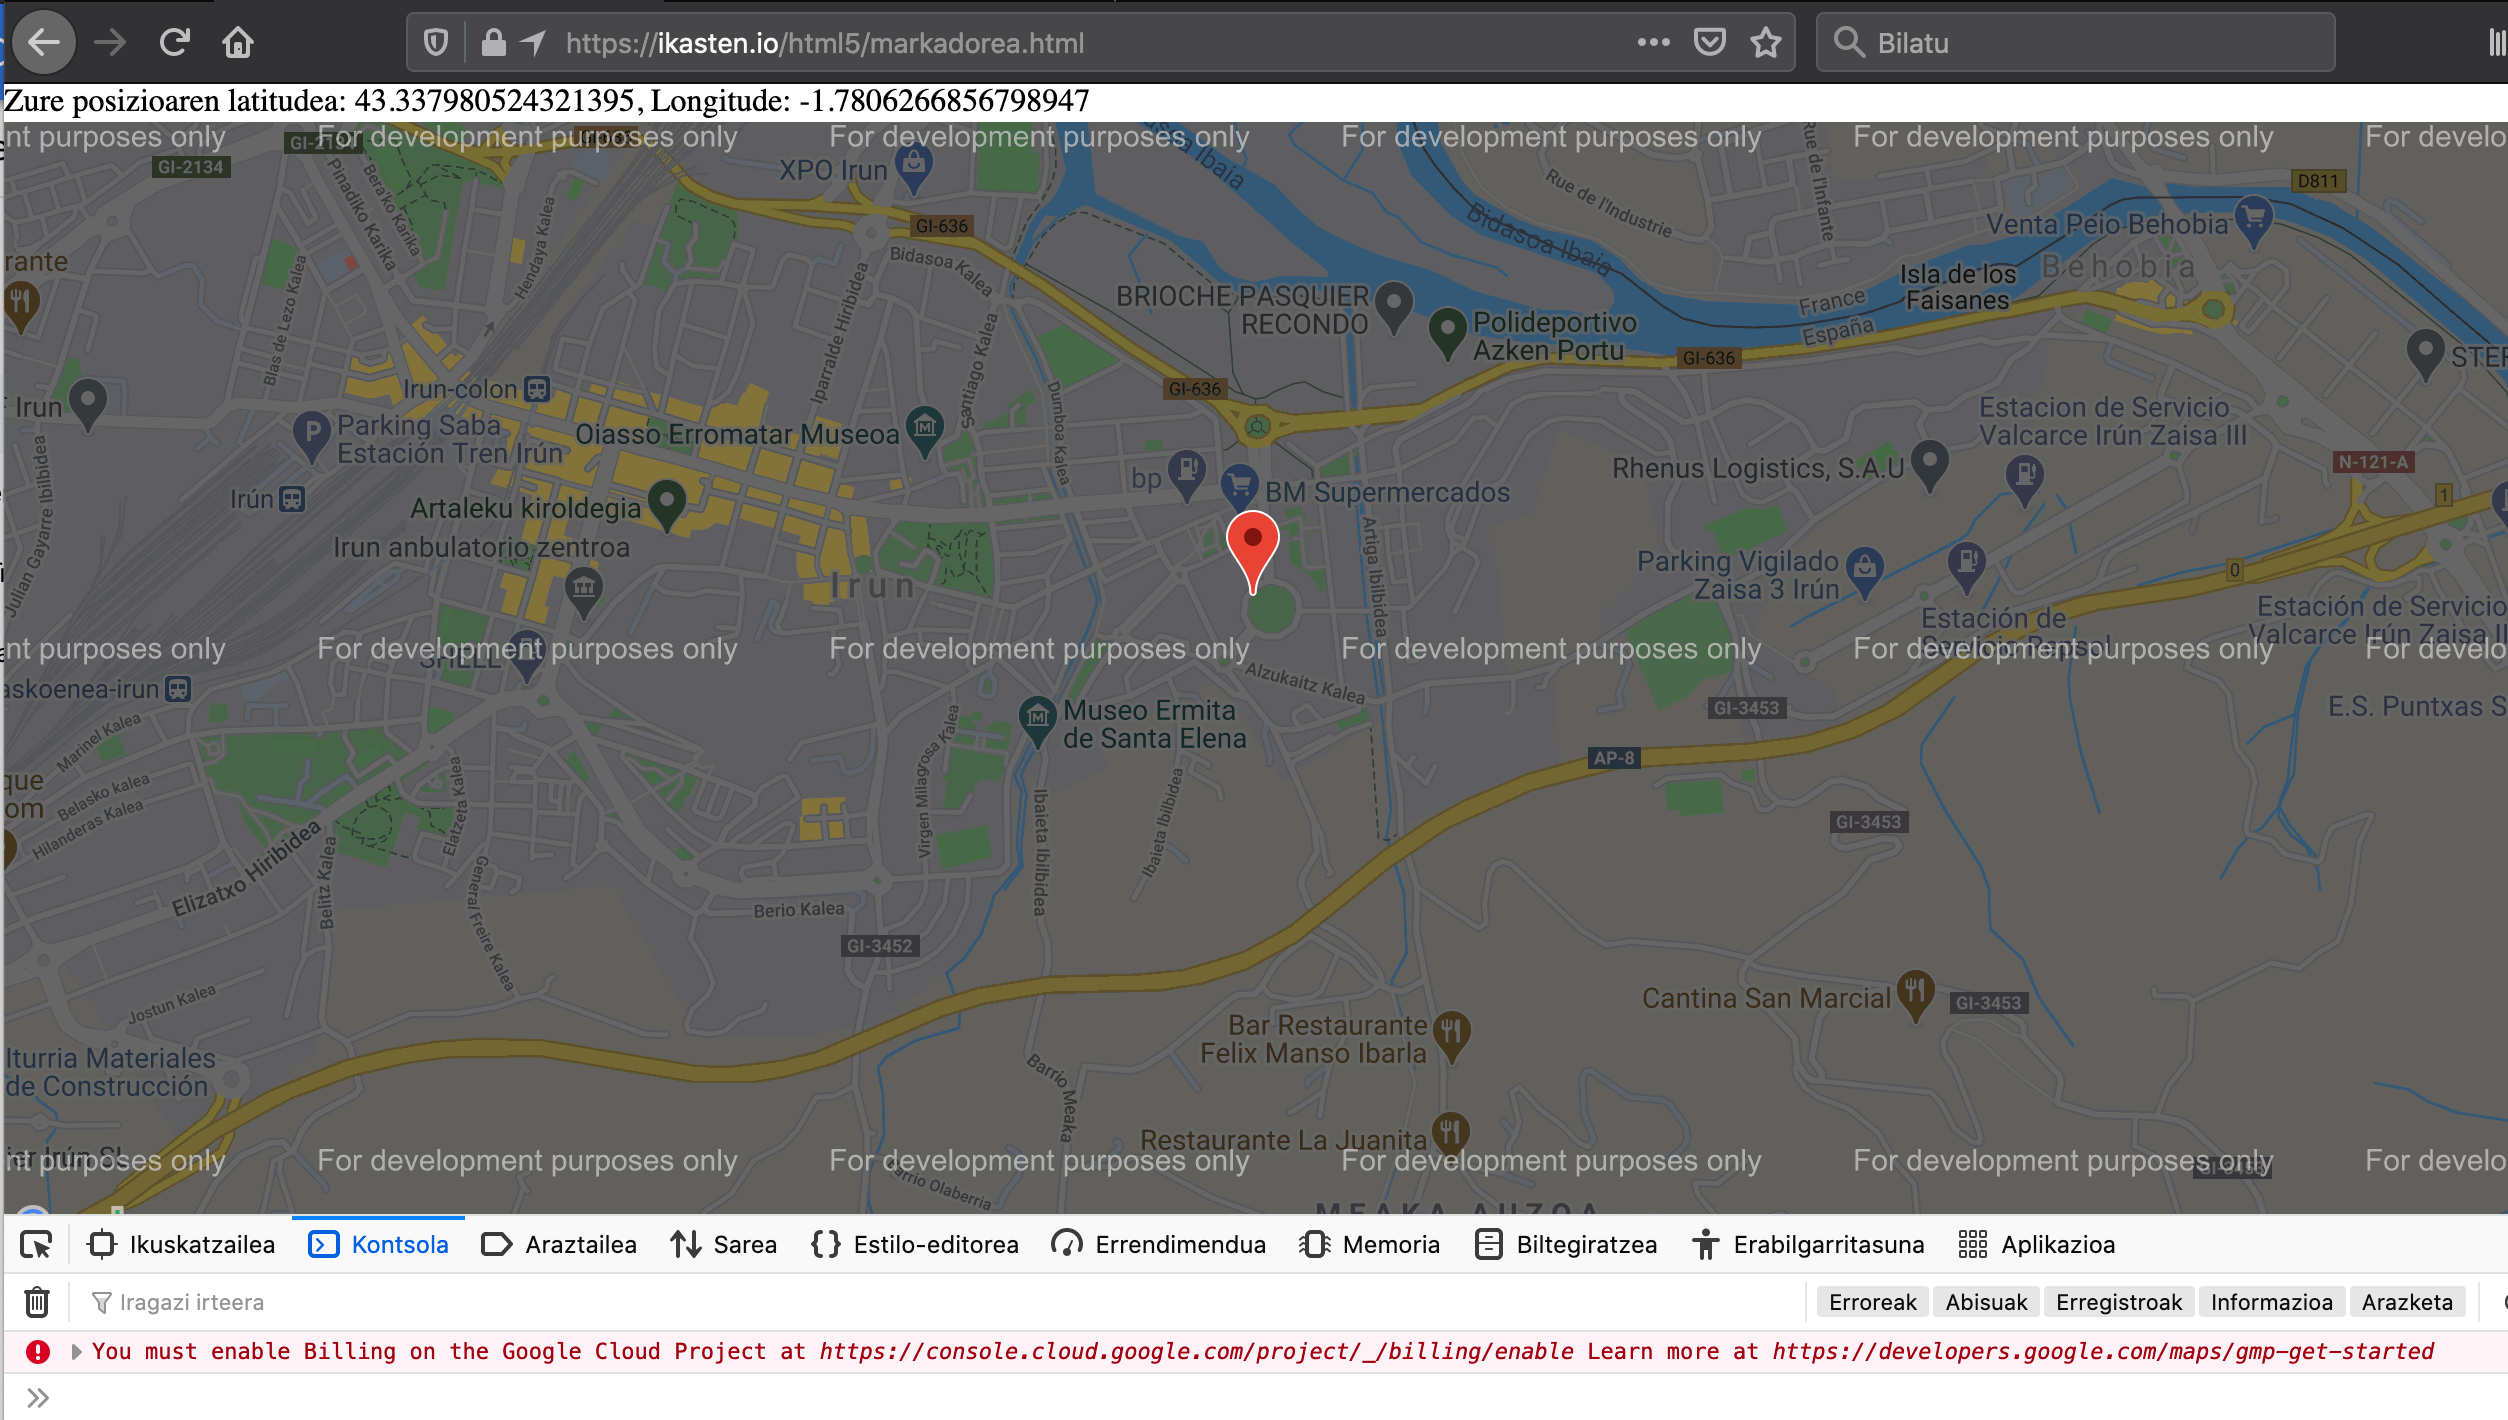
\includegraphics[trim=0cm 0cm 0cm 0cm, clip=true, width=0.75\textwidth]{img/geokokapena/markadorea.png}};
\end{tikzpicture}
\caption{Markatzaileak (mapan agertzen den ikur gorria) Google Maps APIa erabiliz maparen gainean jar daitezke. Ohart zaitez \textit{``For development purposes only''} mezuan eta kontsolan agertzen den mezu gorrian. Mezu horiek kentzeko (eta mapa hobeto ikusteko) ordainpeko kontu bat ireki beharko dugu Google Maps-en honako helbide honetan: \href{https://console.cloud.google.com/project/\_/billing/enable }{https://console.cloud.google.com/project/\_/billing/enable }.}
\label{fig:markadorea}
\end{figure}

\section{Ariketak}

Mugitu ahala zure geokokapena mapa baten gainean bistaratu nahi dugu. Zure geokokapenaren gainean dagoen markatzailean sakatzean, irekitzen den informazio-panelean longitudea eta latitudea bistaratzeaz gain, zauden tokiaren altitudea ere ikusi nahi dugu. Horretarako, Google Maps-ek eskaintzen duen \textit{locationService} APIaren bidez altitudea lortzea eskatzen da. 


Geokokapen APIaren \textit{Coordinates} klaseak hautazko lau parametro eskaintzen ditu (ez daude nabigatzaile guztietan inplementatuta edo ezin dira denak erabili gailu guztietan):
\textit{altitude}, \textit{altitudeAccuracy}, \textit{heading} eta \textit{speed}.

Txantiloi honetan oinarriturik:
\href{https://jsfiddle.net/juanan/jsexk3rh/12/}{https://jsfiddle.net/juanan/jsexk3rh/12/} bertan dagoen JavaScript kodea aldatu markagailu batean klikatzean pantailan uneko posizioa  eta altitudea bistaratu ahal izateko (ikus \ref{fig:maps-ariketa}. irudia). Altueraren datu hori zuzenean eskuratzea posible ez balitz, Google Maps-ek eskaintzen duen elevationService()\footnote{
\textit{elevationService()} metodoaren dokumentazioa hemen aurkituko duzu:\\
\href{https://developers.google.com/maps/documentation/javascript/examples/elevation-simple}{https://developers.google.com/maps/documentation/javascript/examples/elevation-simple}
} zerbitzuari deitu eta hortik eskuratu ahalko duzu\footnote{elevationService() zerbitzutik jasotzen duzun altuera zenbaki erreal gisa bistaratu, bi dezimalera biribilduz (\textit{parseFloat()}\index{parseFloat()} metodoa lagungarria egingo zaizu)}.

\textit{e1elevationService()}\index{elevationService()} metodoa Google Maps-eko 3. bertsiotik aurrera dago eskuragarri. Bertsio
hori nola kargatzen den ikasteko, metodoaren dokumentazioan eskaintzen den adibidearen HTML kodea aztertzea gomendagarria da.


\begin{figure}[ht]
	\centering
\begin{tikzpicture}
\node[anchor=south west,inner sep=0] (image) at (0,0)
   {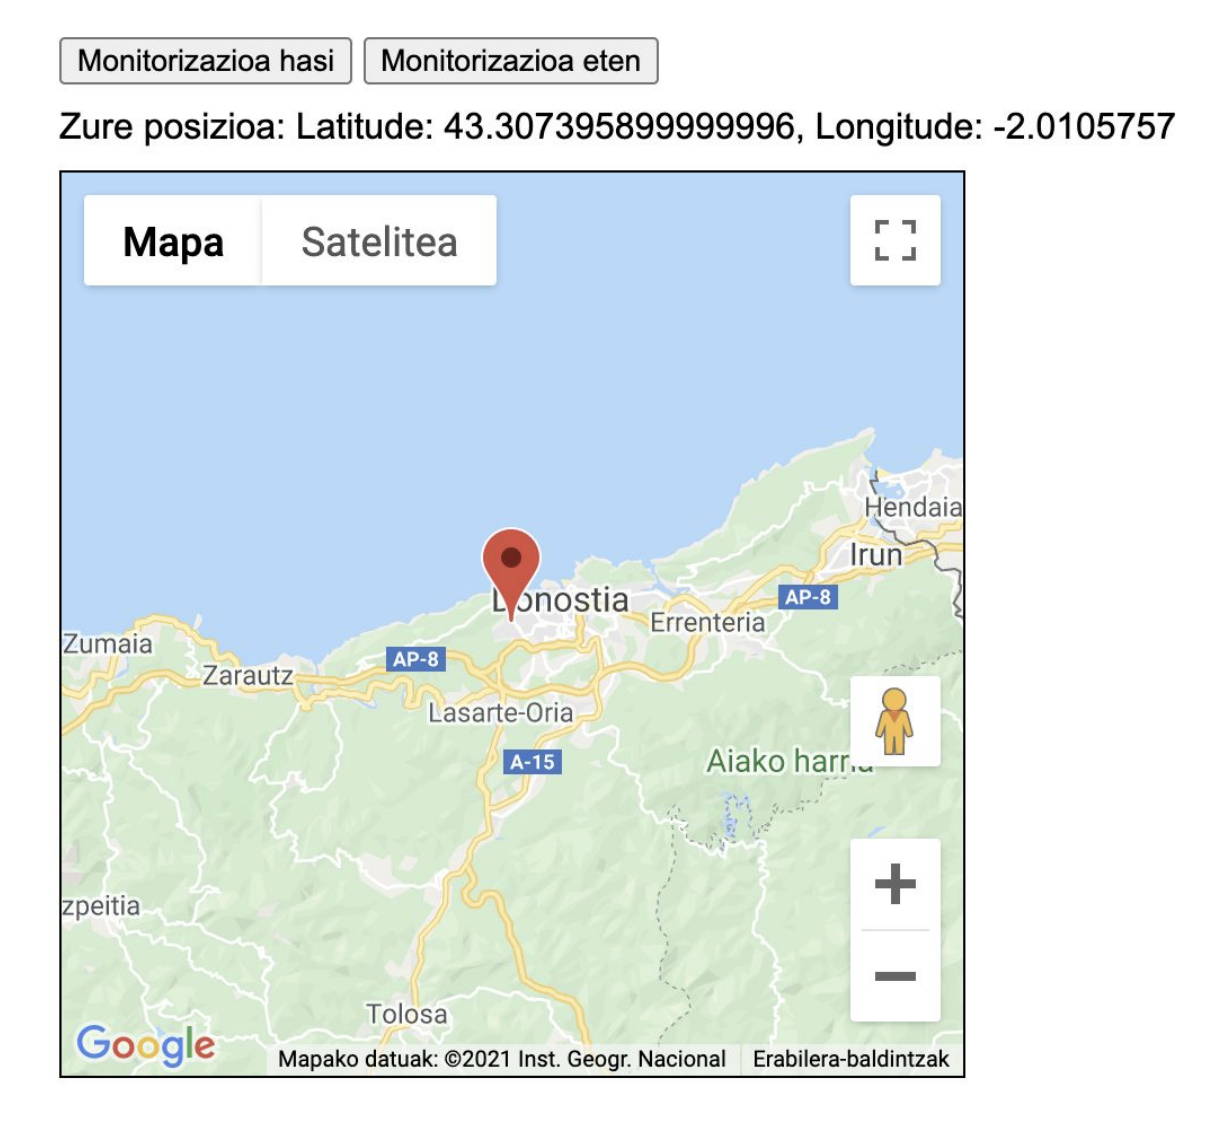
\includegraphics[trim=0cm 0cm 0cm 0cm, clip=true, width=0.5\textwidth]{img/geokokapena/maps-ariketa.png}};
\end{tikzpicture}
\caption{Google Maps-ekin egindako ariketaren emaitza.}
\label{fig:maps-ariketa}
\end{figure}


% \begin{table}[]
% \centering
% \caption{Geokokapen APIak eskaintzen dituen parametro guztiek ez dute derrigorrez balio bat emango. Taulan hautazko eta derrigorrezko atributuak zehazten dira.}
% \label{tab:my-table}
% \begin{tabular}{|l|l|}
% \hline
% \textbf{Coordinates klasea} & \textbf{Geokokapen APIa} \\ \hline
% \begin{tabular}[c]{@{}l@{}}latitude\\ longitude\\ accuracy\end{tabular} & \begin{tabular}[c]{@{}l@{}}Ezker aldeko 3 atributu horiek\\ derrigorrezkoak dira (balio bat itzuli behar\\ dute)\end{tabular} \\ \hline
% \begin{tabular}[c]{@{}l@{}}altitude\\ altitudeAccuracy\\ heading\\ speed\end{tabular} & \begin{tabular}[c]{@{}l@{}}Ezker aldeko 4 atributu horiek hautazkoak\\ dira (batzuetan ez dute baliorik izango)\end{tabular} \\ \hline
% \end{tabular}
% \end{table}

%% 12. Web Worker
\chapter{Web Workers APIa}\index{Web Workers API}
Orain arte, JavaScript erabiliz hari bakarreko programak sortu ditugu. Web Worker APIak JavaScript scriptak aldi berean exekutatzeko ahalmena ematen digu. Hau oso interesgarria da konputazio handiko prozesuak lantzeko. Web Worker-ak existituko ez balira, arazo bat izango genuke, konputazio astun horiek egitean nabigatzailearen interfaze grafikoa blokeatu egingo litzatekeelako: hari bakar batek kalkuluak egin beharko lituzke eta aldi berean ezingo lituzke erabiltzailearen sarrerak kudeatu —saguarekin egindako mugimenduak, botoi-sakatzeak, etab.—.

Kasurik okerrenean nabigatzaileak errore-mezu bat pantailaratuko luke, skript batek kontrola hartu duela eta gainontzeko eragiketa guztiak blokeatu egin direla esateko, skripta amaitzeko aukera emanez (ikus \ref{fig:webworker1}. irudia).

\begin{figure}[ht]
	\centering
\begin{tikzpicture}
\node[anchor=south west,inner sep=0] (image) at (0,0)
   {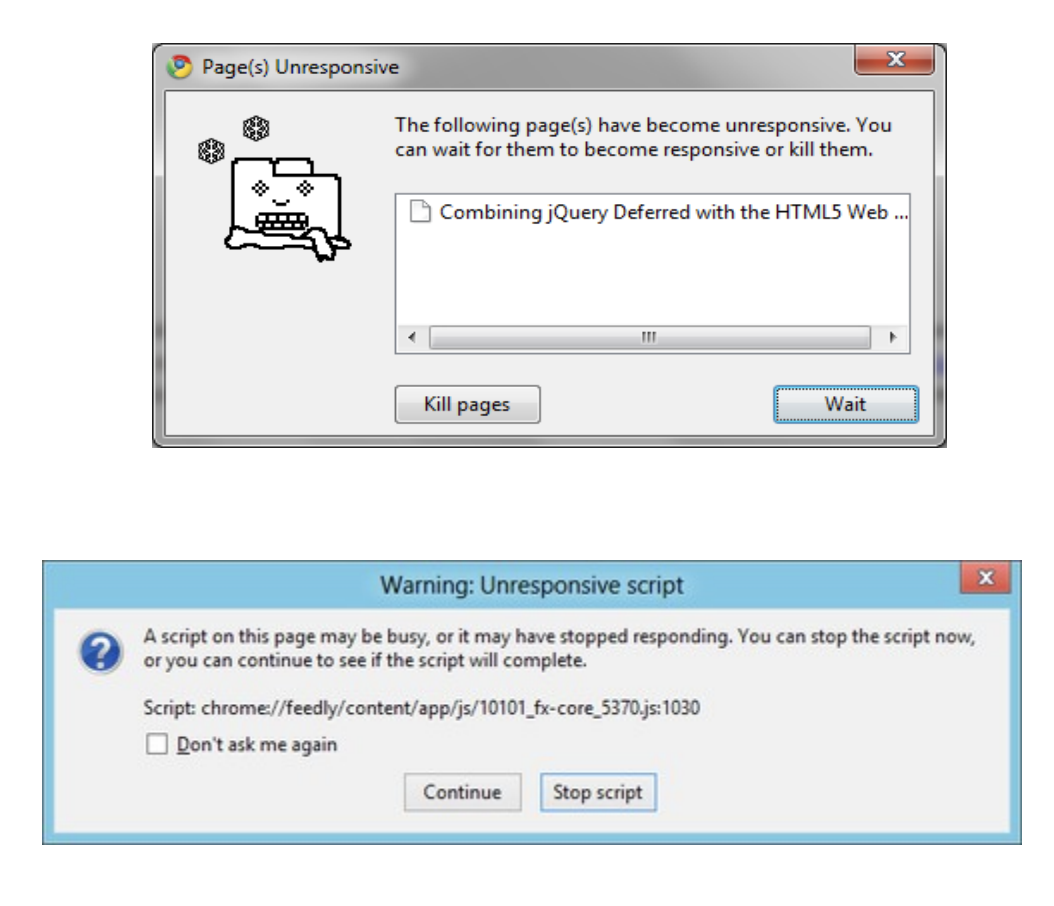
\includegraphics[trim=0cm 0cm 0cm 0cm, clip=true,
   width=0.5\textwidth]{img/page_unresponsive.png}};
\end{tikzpicture}
\caption{Nabigatzaileak exekuzio-denbora luzea behar duen skripta aurkitzen duenean, skript hori amaitu edo itxaroten jarraitu nahi dugun galdetuko digu. Web Worker APIak horrelako errore-mezuak ekiditen lagunduko digu.}
\label{fig:webworker1}
\end{figure}

Web Workers APIa bereziki garrantzitsua da RIA (\textit{Rich Internet Application}) aplikazioetan, aldi berean exekutatzen diren eragiketak egin nahi ditugulako, eta ziur asko horietako batzuk (edo asko) paraleloki egikaritu daitezkeelako, interfaze grafikoaren blokeoa saihestuz. API hau, web aplikazioen elkarreragin arina lortzeko, ezinbestekoa bilaka daiteke gure web aplikazioetan konputazio handiko eragiketak egin behar direnean.

Gai honetan ikusiko dugun Web Workers APIa erabiliz egindako adibideaz gain, John Resig \footnote{John Resig jQuery liburutegiaren sortzailea da. } programatzaileak bere blogean proposatzen dituenak ere aztertzea komeni da.\footnote{\href{http://ejohn.org/blog/web-workers/}{http://ejohn.org/blog/web-workers/}}

\section{Zer da Web Worker bat?}

Laburbilduz, Web Worker bat bigarren planoan exekutatzen den JavaScript programa bat da.

Erabiltzailearen interfaze grafikoa kudeatzen duen JavaScript haria blokeatu gabe, kalkulu-ahalmen handiko atazak exekutatzeko oso egokiak dira.

\section{Zer egin dezakegu Web Workers APIarekin?}

Web Worker-ak honako atazak sortzen dituzten kalkuluak egiteko aukera ezin hobeak dira, adibidez kasu hauetan: 
\begin{itemize}
    \item Jokoak, grafikoak, kriptografia...
    \item Sarrera/Irteera: URL bati \textit{polling} egiteko atzeko planoan.
    \item Web editoreetan erabiltzen den sintaxiaren koloreztatzea lortzeko.
    \item Bigarren planoan exekutatzen diren zuzentzaile ortografikoak.
    \item Online kalkulu-orriak  programatzeko.
    % \item      https://testdrive-archive.azurewebsites.net/Graphics/WorkerFountains/Default.html
    % \item https://msdn.microsoft.com/library/jj635756.aspx (Mandelbrot Fraktalak)
    % \item http://ejohn.org/blog/web-workers
\end{itemize}


\section{Nola erabili Web Worker APIa}

Web Worker berri bat sortzeko \textit{Worker}\index{Worker} klasea instantziatuko dugu:

\begin{lstlisting}[numbers=none]
let worker = new Worker("worker_script.js");
\end{lstlisting}

Web Worker bati mezu bat bidaltzeko \textit{postMessage} metodoa erabiliko dugu \index{postMessage}:
\begin{lstlisting}[numbers=none]
worker.postMessage("Kaixo mundua!");
\end{lstlisting}

Web Worker batek bidaltzen dizkigun erantzunak kudeatu:


\begin{lstlisting}[numbers=none]
worker.onmessage = function(event) {
   console.log("Jasotako mezua: " + event.data);
   zerbaitEgin();
}
\end{lstlisting}


Web Worker bat amaitzeko, berriz, \textit{terminate}\index{terminate} metodoaz baliatuko gara:

\begin{lstlisting}[numbers=none]
worker.terminate();
\end{lstlisting}


\section{Oinarrizko adibidea}

Zenbaki lehenak kalkulatzen lagunduko digun Web Worker bat programatuko dugu adibide honetan.

Lehenengo, lehenaDa() funtzioa programatuko dugu, \hlc[lightgray]{worker.js} fitxategian\footnote{
Adibidearen kodea hemen aurkituko duzu: \href{https://ikasten.io/html5/webworkers/index.html}{https://ikasten.io/html5/webworkers/index.html}}.

\begin{lstlisting}[numbers=none,language=JavaScript]
// worker.js fitxategia
function lehenaDa(n) {
    if (n == 2) return true;
    for (var i = 2; i <= Math.sqrt(n); ++i) {
        if (n % i == 0) return false;
    }
    return true;
}

// amaigabeko begizta batean lehenaDa metodoari
// deitu, 1-etik aurrera dauden zenbaki lehenak
// kalkulatu eta programa nagusiari postMessage 
// erabiliz bidaliko dizkiona
for (var i = 1; ; i++)
    if (lehenaDa(i))
        postMessage(i)
\end{lstlisting}

Jarraian, \textit{worker}-a instantziatu eta \textit{onmessage} metodoaren bidez \textit{worker}-aren mezuak tratatuko ditugu:

\begin{lstlisting}[numbers=none,language=HTML]
<!doctype html>
<html>
<head>
 <title>Web Worker bakar batekin zenbaki lehenak kalkulatzeko adibidea</title>
</head>
<body>
 <p>Kalkulatutako zenbaki lehen handiena: <div id="result"></div></p>
 <script>
 let worker = new Worker('worker.js');
 
 worker.onmessage = function (event) {
       document.getElementById('result').innerHTML = event.data;
 };
 </script>
</body>
</html>
\end{lstlisting}

Aplikazioa martxan jarri eta zenbaki lehenak kalkulatzen dituen bitartean, saguarekin testuaren zati bat hauta dezakegu, nabigatzailearen fitxa itxi, edo nahi duguna egin (\ref{fig:webworker2}. irudia). Programa bera probatzen badugu\footnote{Programa bera, baina Web Worker-ak erabili gabe, hemen aurkituko duzu: \href{https://ikasten.io/html5/webworkers/index2.html}{https://ikasten.io/html5/webworkers/index2.html}. Adi, workerrak erabiltzen direnez, adibide honek nabigatzailea blokeatuko du!} baina Web Worker-ak erabili gabe, nabigatzailea nola blokeatzen den nabarituko dugu (eta kasurik okerrenean ez digu utziko ezta aplikazioaren emaitza ikusi ere  —\ref{fig:webworker3}. irudia—.

\begin{figure}[ht]
	\centering
\begin{tikzpicture}
\node[anchor=south west,inner sep=0] (image) at (0,0)
   {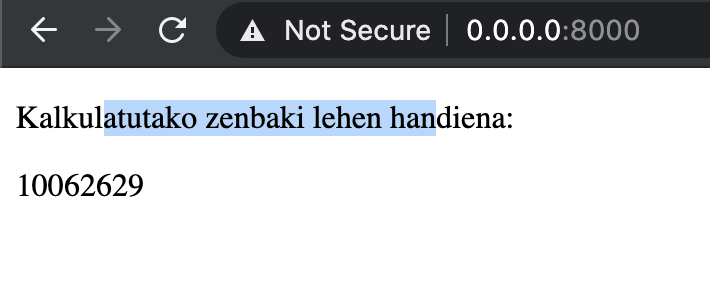
\includegraphics[trim=0cm 0cm 0cm 0cm, clip=true, width=0.5\textwidth]{img/webworkers/worker2.png}};
\end{tikzpicture}
\caption{Web Worker bat erabiliz posible da nabigatzailearekin lan egitea, kalkulu sakonak egiten diren bitartean.}
\label{fig:webworker2}
\end{figure}

\begin{figure}[ht]
	\centering
\begin{tikzpicture}
\node[anchor=south west,inner sep=0] (image) at (0,0)
   {\includegraphics[trim=0cm 0cm 0cm 0cm, clip=true, width=0.5\textwidth]{img/webworkers/webworker3.png}};
\end{tikzpicture}
\caption{Web Worker APIa erabili gabe, orri nagusiak ez du kargatu ere egiten.}
\label{fig:webworker3}
\end{figure}

\section{Ariketak}
Ariketa bakar bat oraingo honetan. Web Worker APIa erabiltzeko \textit{script} baten berridazketa egitea eskatuko zaizu.  \href{https://ikasten.io/html5/webworkers/ww.html}{https://ikasten.io/html5/webworkers/ww.html} orrian dugun skriptak zenbaki lehenak kalkulatzen dituen bitartean \# karakterea inprimatzen du pantailan, behin eta berriro. Web Worker-ik erabiltzen ez duenez, kalkuluak egiten dituen bitartean nabigatzailea erdi blokeatuta geratzen da. Ariketa honen
eginbeharra kodea Web Worker APIa erabiltzeko moldatzea da.

%\href{https://flaviocopes.com/web-workers/}{Web Workers}

%\href{https://medium.freecodecamp.org/how-web-workers-can-help-with-consistent-asynchronous-tasks-in-javascript-cd6d728fa4ee}{How to use Web Workers to schedule consistent asynchronous tasks in JavaScript}

% \href{https://www.youtube.com/watch?v=X57mh8tKkgE}{WebWorkers: Code Session - Supercharged
%}
%%% 13. Inprimakiak
\chapter{Inprimakiak HTML5en}
\index{inprimakiak}\index{form}
HTML4 bertsioan inprimakiak programatzeko hainbat osagai bagenituen ere (\textit{input}, \textit{text}, \textit{numeric}, \textit{select}, \textit{checkbox}, \textit{radiobutton}…), HTML5ek osagai eta atributu berriak ekarri ditu: \index{placeholder}\textit{placeholder}, \index{autofocus}\textit{autofocus}, \index{email}\textit{email} eta \index{url} url —URLak sartzeko eremuak—, zenbakiak sartzeko eremuak (\index{spinbox}\textit{spinbox}, \index{slider}\textit{slider}), datak hautatzeko eremua, kolore bat hautatzeko eremua, bilaketak egiteko kutxak… Berritasun horiek guztiak gai honetan aztertuko dira.

HTMLn, oinarrizko inprimaki baten itxura honakoa da:

\begin{lstlisting}[language=JavaScript]
<form name="inprimakia" action="/kudeatzailea">
   Izena: <input type="text">
   <br><input type="submit">
</form>
\end{lstlisting}


HTML4 bertsioan, inprimakietan erabil zitezkeen eremu motak \ref{tab:my-table}.  taulan zehazten dira.

\begin{table}[]
\resizebox{\textwidth}{!}{% use resizebox with textwidth
\begin{tabular}{lll}
\multicolumn{1}{c}{\textbf{Eremu mota}} & \multicolumn{1}{c}{\textbf{HTML kodea}}                           & \multicolumn{1}{c}{\textbf{Iruzkinak}}             \\ \hline
Kontrol-laukia                          & \textless{}input type="checkbox"\textgreater{}                    & gaitu eta desgaitu daiteke                         \\
Aukera-botoia                           & \textless{}input type="radio"\textgreater{}                       & multzokatu egiten dira                             \\
Pasahitza-eremua                         & \textless{}input type="password"\textgreater{}                    & puntuak idatziko ditu edozein tekla sakatzean \\
Aukera-zerrenda                         & \textless{}select\textgreater{}\textless{}option\textgreater{}... &            \textit{combobox} izenarekin ere ezagutzen dira                                        \\
Fitxategi-eremua                        & \textless{}input type="file"\textgreater{}                        & disko gogorretik fitxategi bat hautatzeko eremua                    \\
Bidaltzeko botoia                       & \textless{}input type="submit"\textgreater{}                      & submit botoia sakatuko dugu inprimakia bidaltzeko \\
Testu-eremua                            & \textless{}input type="text"\textgreater{}                        &            gehien erabiltzen den eremu mota                                        \\ \hline
\end{tabular}
}
\caption{HTML4 bertsioan inprimakietan erabil zitezkeen zenbait eremu mota.}
\label{tab:my-table}
\end{table}

Noski, eremu horiek HTML5en ere erabil daitezke, baina bertsio berri honetan beste eremu mota batzuk sartu ziren, atal honetan aztertuko ditugunak.

\section{Eremu eta atributu berriak HTML5en}

Banan-banan hurrengo atributu eta funtzionalitate berriak landuko ditugu:

\begin{enumerate}
    \item placeholder
    \item autofocus
    \item email eta URLak sartzeko eremuak 
    \item zenbakiak (\textit{spinbox}, \textit{slider})
    \item data bat hautatzeko eremua 
    \item kolore bat hautatzeko eremua 
    \item bilaketak egiteko kutxak 
    \item derrigorrezko eremuak 
    \item inprimakien baliozkotzea
\end{enumerate}

\subsection{Placeholder atributua}
 
 Testu-eremu batean sar daitekeen testu adibide bat bistaratzeko atributua da \textit{placeholder} (ikus \ref{fig:placeholder}. irudia). Adibidez:
 
 \begin{lstlisting}[language=JavaScript,numbers=none]
 <form>
    <input name="q" placeholder="Zure izena">    
    <input type="submit" value="Bidali">
</form>
 \end{lstlisting}
 
 \begin{figure}[ht]
	\centering
\begin{tikzpicture}
\node[anchor=south west,inner sep=0] (image) at (0,0)
   {\includegraphics[trim=0cm 0cm 0cm 0cm, clip=true, width=0.5\textwidth]{img/placeholder.png}};
\end{tikzpicture}
\caption{\textit{Placeholder} atributu motaren adibidea.}
\label{fig:placeholder}
\end{figure}

 \subsection{Autofocus atributua}
 \textit{Autofocus} atributuak duen eremuak fokua hartuko du orria kargatzen denean. Adibidez, google.com kargatzean zuzenean idatz dezakezu bilatu nahi duzuna, inongo eremuan klik egin gabe, bilaketaren testua idazteko eremuak \textit{autofocus} atributua gaituta duelako.
 
 \begin{lstlisting}[language=JavaScript,numbers=none]
 <form>
  <input name="q" autofocus>
  <input type="submit" value="Search">
</form>
 \end{lstlisting}
 
 \subsection{Email eremu mota}
 
 Email eremu mota (\ref{fig:emailmota}. irudia) testu-eremu motakoa bezalakoa da, berezitasun pare batekin: 
 
 \begin{itemize}
     \item Android eta iOS sistema eragileetan teklatu mota aldatzen da bertan klik egitean.
     \item Nabigatzaile batzuek egiaztapen automatikoak egiten dituzte (helbide elektroniko zuzena dela egiaztatzeko).
 \end{itemize}

 \begin{lstlisting}[language=JavaScript,numbers=none]
 <form>
  <input type="email">
  <input type="submit" value="Go">
</form>
\end{lstlisting}
 
 \begin{figure}[ht]
	\centering
\begin{tikzpicture}[framed]
\node[anchor=south west,inner sep=0] (image) at (0,0)
   {\includegraphics[trim=0cm 0cm 0cm 0cm, clip=true, width=0.25\textwidth]{img/email.jpg}};
   \draw [draw=red] (0.70,0.70) rectangle ++(0.3,0.3);
\end{tikzpicture}
\caption{Email motako eremu batean sakatzean, mugikorretan irekitzen den teklatuan, @ karaktereak berezko tekla izango du (testu arruntetan \textit{emojiak} idazteko okupatzen duen tekla).}
\label{fig:emailmota}
\end{figure}

 \begin{figure}[ht]
	\centering
\begin{tikzpicture}[framed]
\node[anchor=south west,inner sep=0] (image) at (0,0)
   {\includegraphics[trim=0cm 0cm 0cm 0cm, clip=true, width=0.75\textwidth]{img/firefoxemailfield.png}};
\end{tikzpicture}
\caption{Nabigatzaileek automatikoki egiaztatzen dute email zuzen bat sartu dela email motako eremu batean.}
\label{fig:emailmota}
\end{figure}

\subsection{URL eremu mota}

URL eremu mota URLak sartzeko erabiliko dugu (adibidez, https://domeinua.eus).
Nabigatzaileak automatikoki egiaztatuko du benetan URL bat dela, hainbat arau betetzen dituela baieztatuz (barra bat / agertzen dela, gutxienez puntu bat, ez duela zuriunerik...)


\subsection{Zenbakiak sartzeko eremuak: \textit{range}, \textit{slider} eta \textit{spinbox} eremu motak}

Zenbakiak \hl{text} edo \hl{range} motako eremuak erabiliz sar daitezke. \index{range}\textit{Range} eremu motan \ref{fig:rangeeremumota}. irudian bistaratzen den bezalako osagai bat izango dugu. Osagai horri \index{slider} \textit{slider} ere esaten zaio. Beste eremu mota bat zenbakiak sartzeko \index{number}\textit{number}  izenekoa da. Mota horri, berriz, \index{spinbox}\textit{spinbox} ere esaten zaio. Bertan soilik zenbakiak sar daitezke eta gezien bidez zenbakia handitu edo gutxitu egin daiteke. Zenbakien arteko jauzia ere kontrola daiteke \index{step}\textit{step} atributuarekin (ikus \ref{fig:numbereremumota} irudia).


 \begin{figure}[ht]
	\centering
\begin{tikzpicture}[framed]
\node[anchor=south west,inner sep=0] (image) at (0,0)
   {\includegraphics[trim=0cm 0cm 0cm 0cm, clip=true, width=0.75\textwidth]{img/range.png}};
\end{tikzpicture}
\caption{\textit{Range} eremu mota.}
\label{fig:rangeeremumota}
\end{figure}

 \begin{figure}[ht]
	\centering
\begin{tikzpicture}[framed]
\node[anchor=south west,inner sep=0] (image) at (0,0)
   {\includegraphics[trim=0cm 0cm 0cm 0cm, clip=true, width=0.75\textwidth]{img/spinbox.png}};
\end{tikzpicture}
\caption{\textit{Number} (edo \textit{spinbox}) eremu mota.}
\label{fig:numbereremumota}
\end{figure}


\subsection{Datak sartzeko eremuak}

 HTML4 bertsioan ez zegoen eremu zehatzik datak sartzeko inprimaki batean; izan ere, JavaScript liburutegi ezberdinak sortu ziren arazo hori konpontzeko (adibidez, \href{https://jqueryui.com/datepicker/}{jQuery DatePicker}\footnote{https://jqueryui.com/datepicker/}). HTML5en, berriz, hainbat osagai ditugu datak eta orduak hautatzeko (\ref{fig:datakorduak}. irudia).
 
 
 \begin{figure}[ht]
	\centering
\begin{tikzpicture}
\node[anchor=south west,inner sep=0] (image) at (0,0)
   {\includegraphics[trim=0cm 0cm 0cm 0cm, clip=true, width=0.65\textwidth]{img/dataetaorduak.png}};
\end{tikzpicture}
\caption{Data eta orduak hautatzeko eremuak.}
\label{fig:datakorduak}
\end{figure}

\subsection{Kolore bat hautatzeko eremu mota}
Kolorea hautatzeko eremua ere berria da HTML5en. Eremuaren izena erraza da: \index{color}\textit{color}. Besterik ezeko balio bat ere eman diezaiokegu. Kolorearen balioa RGB (\textit{red,green,blue}) erabiliz edo zuzenean izen bat esleituz ezar daiteke. Alegia, kolorearen izena gorria bada, \textit{red} izena erabil dezakegu edo haren baliokidea RGB formatuan ``\#ff0000''. 

\index{RGB}RGB formatuak hiru osagai zehazten ditu: gorria, berdea eta urdina koloreen balioak, sistema hamaseitarrean. Berdea adierazteko, adibidez, ``\#00ff00'' erabiliko genuke (edo \hl{ff} baino txikiagoa den beste balio bat berde apalago bat hautatzeko). Noski, oinarrizko koloreak nahastu egin daitezke beste kolore batzuk lortzeko. Adibidez, morea lortzeko kolorea honakoa litzateke: \#ff40ff. Dena den, sistema eragileak berak  \textit{pantone} bezalako kontrol bat eskaintzen du, kolorea grafikoki hautatu ahal izateko, zenbakiak zeintzuk diren jakin gabe (ikus \ref{fig:colorinput} irudia).

\begin{figure}[ht]
	\centering
\begin{tikzpicture}
\node[anchor=south west,inner sep=0] (image) at (0,0)
   {\includegraphics[trim=0cm 0cm 0cm 0cm, clip=true, width=0.65\textwidth]{img/colorinput.png}};
\end{tikzpicture}
\caption{Koloreak hautatzeko \textit{color} eremu mota erabiliko dugu.}
\label{fig:colorinput}
\end{figure}

\subsection{Bilaketak egiteko \textit{search} eremuak}
Bilaketak egiteko \index{search}\textit{search} motako \textit{<input>} osagaiak testu-eremu arruntak bezalakoak dira, erabiltzaileak bertan kontsultak eta bilaketen testua idazteko diseinatuak. Bisualki, berriz, berezitasunak izan ditzake, batez ere mugikorretan bistaratzen badira. Adibidez, Android sistema eragileak lupa baten ikurra jarriko dio Enter teklari (ikus \ref{fig:searchinput}. irudia).

\begin{figure}[ht]
	\centering
\begin{tikzpicture}[framed]
\node[anchor=south west,inner sep=0] (image) at (0,0)
   {\includegraphics[trim=0cm 0cm 0cm 0cm, clip=true, width=0.35\textwidth]{img/searchinput.jpg}};
    \draw [draw=red] (4.95, 0.90) rectangle ++(0.8,0.6);
\end{tikzpicture}
\caption{\textit{Search} eremu motak lupa baten ikurra erabiliko du \textit{Enter} teklan, mugikor batetik bistaratzean.}
\label{fig:searchinput}
\end{figure}

\subsection{Derrigorrezko eremuak (\textit{required})}

\textit{Color} eremu motak aztertzean, \textit{<input>} osagaian \index{required}\hl{required} atributua ikus dezakegu (\ref{fig:colorinput}. irudia). Eremu horretan erabiltzaileak zerbait aukeratu behar duela esan nahi du \textit{required} horrek. Ez badu horrela egiten, nabigatzaileak errore bat jaurtiko du inprimakia bidaltzeko botoian sakatzean eta ez digu bidaltzen utziko arazoa konpondu arte.

\subsection{Inprimakien baliozkotzea}

Inprimaki bat bidaltzean, derrigorrezko (\textit{required}) eremuez gain, eremuen balioak egiaztatu behar dira inprimakia zerbitzarira bidali baino lehen. Eremu jakin batzuen balioa automatikoki konprobatuko da (adibidez, email motakoak, \ref{fig:emailmota}. irudian ikusten den bezala). Beste elementu batzuen balioa, ordea, skript baten bidez egiaztatu beharko ditugu. Adibidez, demagun \ref{fig:datakorduak}. irudian data eta ordu bat hautatzean, erabiltzaileak soilik lanegunak direnak aukeratu ditzakeela, eta soilik 10:00-14:00 ordu-tartean. Aukeraketa hori zuzena ez bada, errore-mezu bat pantailaratuko dugu, arrazoia azalduz.

Kodea \ref{lst:inprimakiaegiaztatu}. listatuan aurkezten da. Bertan \textit{form} etiketari \index{onsubmit}\textit{onsubmit} kudeatzaile bat esleitu zaio. Kudeatzaile horrek boolear bat bueltatu behar du: dena ondo badago inprimakian,  \textit{true} (eta inprimakia zerbitzarira bidaliko da, haren \textit{action} atributua zehazten duen helbidera), eta erroreren bat aurkituz gero, \textit{false} (eta, beraz, ez da inprimakia zerbitzarira bidaliko).

\begin{figure}[ht]
	\centering
\begin{tikzpicture}[framed]
\node[anchor=south west,inner sep=0] (image) at (0,0)
   {\includegraphics[trim=0cm 0cm 0cm 0cm, clip=true, width=0.5\textwidth]{img/formegiaztatu.png}};
\end{tikzpicture}
\caption{Inprimaki baten balioak egiaztatu ondoren errore bat pantailaratu dezakegu beharrezkoa bada.}
\label{fig:searchinput}
\end{figure}

\clearpage
%\begin{minipage}[t][.8\textheight][s]{\textwidth}
\begin{lstlisting}[language=JavaScript,caption={Inprimaki baten balioak egiaztatzeko kodea.},captionpos=b]
<script>
    function egiaztatu(){
        const inprimakia = document.getElementById('inprimakia');
        // ordua:minutua formatuan dagoen string batetik ordua lortu
        const ordua = inprimakia.ordua.value.split(":")[0];
        // eguna lortu (string bat date datu motan bihurtu)
        const eguna = new Date(inprimakia.data.value);
        let erroreak = '';
        // 6 = larunbata 0 = igandea 1 = astelehena ...
        if (eguna.getDay() == 6 || eguna.getDay() == 0) {
            erroreak += 'Asteburu bat aukeratu duzu';
        }
        // ordua 10-14 tartean egon behar da
        if (ordua < 10 || ordua > 14) {
            erroreak += '<br>Soikik 10etatik 14etara gaude zabalik';
        }
        if (erroreak != ''){
            document.getElementById('erroreak').innerHTML = erroreak;
            return false;
        }
        return true;
    }
</script>
</head>
<body>

<div id="erroreak"></div>
<form id="inprimakia" method="POST" action="/inprimakia" onsubmit="return egiaztatu();" >
\end{lstlisting}
\label{lst:inprimakiaegiaztatu}
%\end{minipage}

\section{Ariketak}

Sor ezazu \ref{fig:inprimakiak}. irudian dagoen inprimakia HTML5ek eskaintzen dituen eremu berriak erabiliz eta honako arauak kontuan hartuz:

\begin{figure}[ht]
	\centering
\begin{tikzpicture}[framed]
\node[anchor=south west,inner sep=0] (image) at (0,0)
   {\includegraphics[trim=0cm 0cm 0cm 0cm, clip=true, width=0.5\textwidth]{img/inprimakiak/inprimakia.png}};
\end{tikzpicture}
\caption{Erabiltzaileak datuak idatzi ostean \textit{Bidali} botoian  sakatuko du. Akatsik balego, jakinaraziko zaio.}
\label{fig:inprimakiak}
\end{figure}

\begin{itemize}
    \item Izena eremuak orria kargatzean fokua hartu behar du.

\item Telefonoa eremua ez da orain arte agertu, baina gai
izango zinateke programatzeko? Eta telefono baten
patroia automatikoki antzemateko? (Argibidea: ikus \textit{regex} patroiak
HTML5en)

\item Ohart zaitez eremu batzuetan txantiloi gisa zerbait agertzen dela aurreidatzita (\textit{placeholder} bat).

\item Liburuak izeneko eremuan klik bikoitza egitean 5 libururen izenak agertu behar dira (ikus \textit{Datalist} HTML5en).
\end{itemize} 
%% 14. WebSocketak
\chapter{WebSocket-ak}

\index{WebSocket}WebSocket-ak jaio baino lehen, bezeroak zerbitzaritik datu bat jaso nahi zuenean, \index{AJAX}AJAX bidez egin behar zuen eskaera (\index{XmlHttpRequest}XmlHttpRequest edo \index{XHR}XHR objektu bat sortuz edo Fetch APIa erabiliz). Baliabide bakoitzeko XHR konexio bat ireki behar da: irudi bat lortzeko, JavaScript fitxategi bat atzitzeko, HTML orri bat jaisteko... 
Gauza bera bezeroak zerbitzarian dagoen prozesu baten egoera ezagutu nahiko balu:  une oro XHR eskaerak egin beharko lituzke (\textit{polling} delakoa\index{polling}). Prozedura hori ez da batere eraginkorra. Hoberena izango litzateke bezeroa entzuten jartzea eta zerbitzariak, noizbait bezeroari jakinarazi behar dion gertaeraren bat ikustean, bezeroari mezu bat bidaltzea. Hori da hain zuzen ere WebSocket APIaren zeregin nagusia. 

WebSocket-a ordenagailuen arteko \textit{full-duplex} edo bi norabideko komunikazioa lortzeko protokolo bat da, TCP konexio bakar baten gainean.

Horretaz aparte, nabarmendu daitekeen beste abantaila bat zera litzateke: WebSocket bat eraiki ondoren, bertatik bidaltzen diren pakete-goiburuen tamaina HTTP protokoloan erabiltzen direnena baino askoz txikiagoa da (ikus \ref{fig:wsheader}. irudia).


\begin{figure}[ht]
	\centering
\begin{tikzpicture}
\node[anchor=south west,inner sep=0] (image) at (0,0)
   {\includegraphics[trim=0cm 0cm 0cm 0cm, clip=true, width=1.0\textwidth]{img/http_header.png}};
\end{tikzpicture}
{\includegraphics[trim=0cm 0cm 0cm 0cm, clip=true, width=0.5\textwidth]{img/ws_header.png}}
\caption{HTTPn pakete-goiburuen tamaina (goiko aldean, 1.356 byte) WebSocket protokoloan erabiltzen direnena (beheko aldean, 247 byte) baino askoz handiagoa da.}
\label{fig:wsheader}
\end{figure}


 WebSocket APIaz, HTTP zerbitzari baten kontra konexio bat ireki eta bertatik datuak jaso edo bidali ahal izango ditugu.  Zerbitzariak datu berriak bidali nahi dituenean, zuzenean egingo du, bezeroak ezer eskatu gabe. Horrez gain, WebSocket zerbitzari batek hainbat bezerorekin konexio irekiak izan ditzake aldi berean, bakoitzarekin \textit{socket} bat irekiz, komunikazioa denbora errealean garatuz. Gaur egun, HTML5en programatutako bideo-joko eta aldibereko talde-lana egiteko tresna askotan WebSocket-ak erabiltzen dira komunikazio eraginkorra lortzeko. Adibidez, Google Driven, dokumentu bat hainbat pertsonaren artean aldi berean editatzen dugunean, edo \ref{fig:whiteboard}. irudian ikusten dugun arbel digital partekatuan, WebSocket APIa erabiltzen ari gara.
 
 
\begin{figure}[ht]
	\centering
\begin{tikzpicture}
\node[anchor=south west,inner sep=0] (image) at (0,0)
   {\includegraphics[trim=0cm 0cm 0cm 0cm, clip=true, width=1.0\textwidth]{img/whiteboardws.png}};
\end{tikzpicture}
\caption{WebSocket protokoloa erabiliz arbel digital partekatu bat programatu dezakegu, aldi berean hainbat erabiltzaileri bertan margotzeko aukera eskainiz. Iturria: \href{http://www.unionplatform.com/?page\_id=2762}{http://www.unionplatform.com/?page\_id=2762}.}
\label{fig:whiteboard}
\end{figure}


\section{WebSocket APIa nola erabili}

\subsection{Socket berri bat sortu (bezeroan)}

WebSocket-ek \index{ws}ws (edo \index{wss}wss, WebSocketSecure) protokoloa erabiliko dute HTTP edo HTTPS protokoloaren ordez.

Bezeroak socket-konexio berri bat sortu nahi duenean, WebSocket klasea instantziatuko du.

\begin{lstlisting}[language=JavaScript,numbers=none]
    let socket = new WebSocket("ws://domeinua/zerbitzua")
\end{lstlisting}

\subsection{Konexioa ezarri}

 Socketa irekitzean \textit{open} gertaera altxatuko da. Hori kudeatzeko \textit{socket.onopen} kudeatzailea zehaztuko dugu \index{onpen}:

 \begin{lstlisting}[language=JavaScript,numbers=none]
 socket.onopen = function(){
  console.log("Konexioa lortu da!");
}
\end{lstlisting}

\subsection{Mezuak jaso eta bidali}

Bezerotik zerbitzarira mezuak bidaltzeko \index{send}\textit{send} metodoaz baliatuko gara:

\begin{lstlisting}[language=JavaScript,numbers=none]
socket.send("mugimendu zuzena");
\end{lstlisting}

Bezeroak zerbitzaritik datozen mezuak entzuteko \index{onmessage}\textit{onmessage} izeneko \textit{callback} bat prestatuko du:

\begin{lstlisting}[language=JavaScript,numbers=none]

socket.onmessage = function(erantzuna) {
   console.log("Jasotako erantzuna: " + erantzuna.data);
}
\end{lstlisting}

Gaur egun ez da WebSocket APIa zuzenean programatzen, baizik eta horren ordez ospetsua egin den \index{socket.io}socket.io izeneko liburutegia erabiltzen da. Liburutegi hori bezeroan kargatzea erraza da:

\begin{lstlisting}[language=HTML,numbers=none]
    <script type="text/javascript" src="/socket.io/socket.io.js"></script>
\end{lstlisting}

Jabetu zaitez /socket.io/ karpetaren izena dela. Bertan dagoen \hl{socket.io.js}
fitxategiak gordetzen ditu erabil ditzakegun funtzioak, \textit{io} objektua barne. 

Hurrengo adibidean, \textit{socket.io} liburutegiaz baliatuko gara WebSocket konexio bat irekitzeko (\textit{connect} metodoaz). Jarraian \textit{socket}-etik mezuak bidaltzeko \index{emit}\textit{emit} metodoa erabiliko dugu.  Zerbitzaritik mezu bat jasotzean, \textit{socket.on} bidez zer funtzio egikarituko den zehazten da. Funtzioa jaso den mezuaren edukiaren arabera zehazten da. Adibidean, \hl{socket.on(\textquotesingle{}mugi\textquotesingle{})} dugu, baina baita \hl{socket.on(\textquotesingle{}phone-connect\textquotesingle{})} mezu mota ere. 

\begin{lstlisting}[language=JavaScript,numbers=none]
const serverURL = window.location.host;

// websocket zerbitzarira konektatu
export const socket = io.connect(serverURL);

// socket-atik mezu bat bidali
socket.emit('desktop-connect');

// socket-atik "mugi" mezu mota datorrenean
// mugitu metodoari deitu
socket.on('mugi', mugitu);

// socket-atik "phone-connect" mezu mota datorrenean
// phoneConnected metodoari deitu
socket.on('phone-connect', phoneConnected);

\end{lstlisting}

Zerbitzariaren aldetik, kodea oso antzekoa da.

\begin{lstlisting}[language=JavaScript,numbers=none]

const io = require('socket.io')(3000);

io.on('connection', socket => {
  // posible da mezu bat zuzenean bidaltzea
  socket.send('Hello!');

  // edo emit() bidez, gertaera zehatz batzuk bidaltzea
  socket.emit('mugi', {'nondik': 12, 'nora': 14});

  // bezeroak  socket.send() erabiliz gertaera bat bidali digu. Hori kudeatzeko:
  socket.on('message', (data) => {
    console.log(data);
  });

  // desktop-connect mezu mota jasotzean, kontsolan mezu bat bistaratuko dugu
  socket.on('desktop-connect', () => {
    console.log("Parametrorik gabeko deia");
  });
});

\end{lstlisting}

Zerbitzarian socket.io instalatzeko, \hl{npm} komando hau erabiliko dugu:
\begin{lstlisting}[language=Bash,numbers=none]
npm install socket.io
\end{lstlisting}

Oharra: npm, nodejs eta orokorrean zerbitzariaren aldeko kodearen inguruan beste liburu bat idatz daiteke. Nolanahi ere, honen inguruan oinarrizko ezagutza beharrezkoa ikusten denez, NodeJS-ri buruzko kapitulu bat eskaini da liburu honetan (ikus  \ref{chap:nodejs}. kapitulua).)

Zerbitzarian ez dugu soilik WebSocket bat izango, baizik eta hasierako HTTP protokoloa kudeatzeko zerbitzu bat ere eskaini behar dugu. Dena batera egin ahal izateko aurreko kodea apur bat aldatu beharra dago, honela:

\begin{lstlisting}[language=JavaScript,numbers=none]

const content = require('fs').readFileSync(__dirname + '/index.html', 'utf8');

const httpServer = require('http').createServer((req, res) => {
  // index.html orria zerbitzatu 
  res.setHeader('Content-Type', 'text/html');
  res.setHeader('Content-Length', Buffer.byteLength(content));
  res.end(content);
});

const io = require('socket.io')(httpServer);

io.on('connection', socket => {
  // posible da mezu bat zuzenean bidaltzea
  socket.send('Hello!');

  // edo emit() bidez, gertaera zehatz batzuk bidaltzea
  socket.emit('mugi', {"nondik": 12, "nora": 14});

  // bezeroak  socket.send() erabiliz gertaera bat bidali digu. Hori kudeatzeko:
  socket.on('desktop-connect', (data) => {
    console.log(data);
  });

});


httpServer.listen(3000, () => {
  console.log('go to http://localhost:3000');
});


\end{lstlisting}

Bezeroaren azken bertsioa, berriz, honela:

\begin{lstlisting}[language=HTML,numbers=none]
<!DOCTYPE html>
<html>
<head>
	<script type="text/javascript" src="/socket.io/socket.io.js"></script>
</head>

<body>

 <ul id="events"></ul>

	<script>
	
		// funtzio laguntzailea
		const $events = document.getElementById('events');
		const newItem = (content) => {
		  const item = document.createElement('li');
		  item.innerText = content;
		  return item;
		};


		// zerbitzariaren URLa
		const serverURL = window.location.host;
	
		console.log(serverURL);

		// websocket zerbitzarira konektatu
		const socket = io.connect(serverURL);

		// konexioa lortzean funtzio laguntzaileari deitu eta pantailan idatzi
		socket.on('connect', () => {
		console.log("Connect");
		  $events.appendChild(newItem('connect'));
		});

		// socket-atik mezu bat bidali
		socket.emit('desktop-connect', {"datuak": "adibide bat"});

		// socket-atik "mugi" edo "phone-connect" mezu mota datorrenean
		// newiItem metodoari deitu
		socket.on('mugi', (datuak) => {
					$events.appendChild(newItem(JSON.stringify( datuak)));
				});
	</script>


</body>
</html>
\end{lstlisting}

Adibidea probatzeko, terminal bat ireki eta, bertatik, \hlc[lightgray]{node server.js} komandoa landu.

Dena ondo badoa, http://localhost:3000 helbidean HTTP eta WS zerbitzaria entzuten egongo dira. Nabigatzailea irekitzean \ref{fig:websocketadibidea}. irudian ikusten dena ikusi beharko genuke. Bertan, dagoen lehenengo \textquotesingle{}connect\textquotesingle{} lerroa bezeroak zerbitzariaren kontra konexioa ondo irekitzean idatziko da. Hurrengo lerroa, berriz, zerbitzaritik \textquotesingle{}mugi\textquotesingle{} gertaera jasotzean agertuko da (gertaera horren barruan dauden datuak bistaratuz).

\begin{figure}[ht]
	\centering
\begin{tikzpicture}
\node[anchor=south west,inner sep=0] (image) at (0,0)
   {\includegraphics[trim=0cm 0cm 0cm 0cm, clip=true, width=.75\textwidth]{img/websockets/websocket.png}};
\end{tikzpicture}
\caption{WebSocket-en adibidea martxan jartzean horrelako emaitza lortu beharko genuke.}
\label{fig:websocketadibidea}
\end{figure}

Adibidearen kode osoa hemen aurkituko duzu:
\href{https://gist.github.com/juananpe/06df4742dae0cc01351089b5bed4c641}{https://labur.eus/5cEjB} (github.com).

\section{Ariketak}
WebSocket-ak eta mugikor bat erabiliko ditugu urruneko aginte bat programatzeko. Zehazki, pantailan grafiko bat bistaratuko da eta mugikorra eskuin aldera biratzean grafikoa eskuinera mugitu behar da. Ezkerrera biratzean, aldiz, grafikoa ezker aldera mugituko da (ikus \ref{fig:websocketariketa}. irudia).

\begin{figure}[ht]
	\centering
\begin{tikzpicture}
\node[anchor=south west,inner sep=0] (image) at (0,0)
   {\includegraphics[trim=0cm 0cm 0cm 0cm, clip=true, width=1.0\textwidth]{img/websockets/websocketariketa.png}};
\end{tikzpicture}
\caption{WebSocket-ak erabiliz mugikor batetik kontrolatu dezakegu pantailan agertzen den irudi bat, ezker-eskuinera mugituz, mugikorra alde batera edo bestera biratzean.}
\label{fig:websocketariketa}
\end{figure}

Mugikorraren biraketak kontrolatzeko kodea hemen aurkituko duzu:\newline
\href{https://www.dropbox.com/s/dh81ca4f9isb44g/sockets\_mobile.zip?dl=1}{https://labur.eus/evkQ2} (dropbox.com).

Zerbitzariaren kode-txantiloia ere lagungarria aurkituko duzu: \href{https://gist.github.com/juananpe/6c27962e19163adb1bd145298d9ec611}{https://labur.eus/J9van} (github.com). NodeJS-n programatuta dago, beraz, ondo ulertzeko liburu honen NodeJS-ri buruzko gaia aztertzea gomendagarria da.
%%% 15. Service Worker APIa
\chapter{Zerbitzu-langileak (Service Worker-ak)}
\index{Service Worker}
Service Worker-a (SW) nabigatzailean, atzeko planoan eta web orririk gabe exekutatzen den \mbox{script} bat da. Script hauek egikaritzeko ez da behar ez erabiltzailearen interakziorik ezta web orririk ere. Ezaugarri horri esker, Service Worker-ak Interneteko konexiorik gabe geratzen garenean erabiltzaileari beste zerbait eskaintzeko erabil ditzakegu. Adibidez, demagun erabiltzailea inprimaki batean mezu bat idazten ari denean konexioa galdu egiten duela. Idazten ari zen mezu hori bidali nahiko balu, inprimakian bidali botoian sakatu eta... mezua galdu egingo du! Ez badugu ezer programatzen egoera hori ekiditeko, mezua galdu egingo da erabiltzailea konexiorik gabe baitago. Hemen sartzen da Service Worker APIa. SW batek konexiorik ez dagoela antzeman dezake eta mezua nabigatzailearen katxean gorde, erabiltzaileari ohartaraziz konexiorik gabe dagoela (baina mezua ez duela galdu). Konexioa berriro lortzean Service Worker-ak egoera berria antzeman eta gordeta zituen mezu guztiak zerbitzarira bidal ditzake (sinkronizazioa lortuz). Gai honetan, hain zuzen ere, deskribatutako konexiorik gabeko (\textit{offline}\index{offline}) egoera hori kudeatzen ikasiko dugu.

\section{Service Worker-ak nola erabili}

Gure adibidea prestatuko dugu. Hasteko, webgune bat kargatzean, konexioa baldin badago, \ref{fig:serviceworker1}. irudiko egoera bistaratu nahiko dugu, alegia, ikur bat eta konexioa dagoela dioen mezu bat.
\begin{figure}[ht]
	\centering
\begin{tikzpicture}
\node[anchor=south west,inner sep=0] (image) at (0,0)
   {\includegraphics[trim=0cm 0cm 0cm 0cm, clip=true, width=0.75\textwidth]{img/online.png}};
\end{tikzpicture}
\caption{Service Worker-a konexioa dagoenean kargatzen da eta nabigatzailearen atzeko planoan exekutatzen geratzen da (egoiliar).}
\label{fig:serviceworker1}
\end{figure}

Baina konexioa galtzean, erabiltzaileak orri bera kargatzen badu, \ref{fig:serviceworker2}. irudian agertzen den ikurra eta mezua ikustea nahiko dugu.

\begin{figure}[ht]
	\centering
\begin{tikzpicture}
\node[anchor=south west,inner sep=0] (image) at (0,0)
   {\includegraphics[trim=0cm 0cm 0cm 0cm, clip=true, width=0.75\textwidth]{img/offline.png}};
\end{tikzpicture}
\caption{Service Worker bat probatzeko konexioa eten egin behar dugu. Horretarako Chrome-k Network fitxan \textit{Offline} egoerara jauzi egiteko aukera ematen du.}
\label{fig:serviceworker2}
\end{figure}

Service Worker-a hasierako orria kargatzean nabigatzailearen atzeko planoan geratzen da egoiliar. Hortik, \index{proxy} \textit{proxy} baten lanak egiten ditu (\ref{fig:serviceworker3}. irudia) Hau da, web aplikazioak HTTP(s) eskaera bat egiten duenean SWatik igaroko da eta horrek hortik aurrera konexioak monitorizatuko ditu, proxy baten lanak eginez. Konexioa badago (\textit{online} egoeran bagaude), SWa gardena izango da, dagokion webgunetik baliabidea eskatuko du eta aplikazioari itzuliko dio. Konexioa galtzen bada (\textit{offline} egoera), alternatiba bat \textit{cache} batetik jasoko du eta hori izango da aplikazioan bistaratuko dena. Hurrengo ataletan prozesu hau nola inplementatzen den ikasiko dugu.

\begin{figure}[ht]
	\centering
\begin{tikzpicture}
\node[anchor=south west,inner sep=0] (image) at (0,0)
   {\includegraphics[trim=0cm 0cm 0cm 0cm, clip=true, width=0.75\textwidth]{img/serviceworker3.png}};
\end{tikzpicture}
\caption{Service Worker batek proxy-aren lanak egiten ditu \textit{fetch} eskaerak antzematen. Konexioa dagoenean, urruneko zerbitzariari birbidaliko dizkio eskaerak. Ez dagoenean, \textit{cache} batetik jasoko ditu. Iturria: \href{https://auth0.com/blog/creating-offline-first-web-apps-with-service-workers/}{https://auth0.com/blog/creating-offline-first-web-apps-with-service-workers/}.}
\label{fig:serviceworker3}
\end{figure}

\section{Konexiorik gabeko aplikazioak}

Aipatutako konexiorik gabeko aplikazioa lortzeko, hiru fasetan banatuko ditugu eman beharreko pausoak:

\begin{itemize}
    \item SWa instalatu eta \textit{cache}an \textit{offline} orria txertatu (\textit{offline} egoeran ikusi behar den orriaren kopia bat).
    \item Erabiltzailea konexiorik gabe nabigatzen saiatzen bada, \textit{cache}an dagoen orria itzuli.
    \item Erabiltzaileak konexioa izanik orrian nabigatzen badu, zerbitzaritik jasoko du orriaren edukia (SWrik egongo ez balitz bezala).
\end{itemize}

\section{Service Worker-a instalatu}

Service Worker-a instalatzeko honako scripta erabiliko dugu.

\begin{lstlisting}[language=JavaScript]
<script>
		// Service Worker-a erregistratu
		if ('serviceWorker' in navigator) {
			navigator.serviceWorker.register('./service-worker.js')
			.then(function(registration) {
		        // Ondo erregistratu da
		        console.log('ServiceWorker-a irismen honekin erregistratu da: ', registration.scope);
		}).catch(function(err) {
		    // Erregistroak kale egin du  :(
		    	console.log('ServiceWorker-a ezin izan da erregistratu: ', err);
		    });
		}
	</script>
\end{lstlisting}
\index{scope}
Bertan ServiceWorker-a uneko nabigatzailean onartzen den edo ez egiaztatu ondoren (3. lerroa), erregistratu egiten da, promes baten bidez. Erregistratzeko\index{register} \hl{navigator.serviceWorker.register} metodoa erabiliko dugu. Metodo horrek parametro gisa SWaren kodea duen scriptaren bidea jasoko du. Parametro hori garrantzitsua da. Adibidean, \textquotesingle{}./\textquotesingle{} (uneko katalogoa); alegia, uneko karpetaren barruan egiten diren eskaerak monitorizatuko dituela soilik (haren irismena \textquotesingle{}./\textquotesingle{} dela esango dugu). Edo teknikoki, \textit{fetch}\index{fetch} gertaerak soilik \textquotesingle{}./\textquotesingle{} karpetan monitorizatuko direla. Horren ordez, bidea  \hl{/adibidea/service-worker.js} izango balitz, irismena soilik \hl{/adibidea/} karpetaren barrukoa izango litzateke.

SW bat hainbat aldiz erregistratzen saiatuz gero, ez da ezer gertatuko (nabigatzaileak behin bakarrik erregistratuko du).  

\section{ServiceWorker-a programatzen}

SWa programatzeko garbi izan behar dugu haren funtzionamendua (ikus \ref{fig:serviceworker4}. irudia). ServiceWorker bat irismen baten barruan erregistratu ondoren, irismen horren barruan dagoen eskaera berriak jasotzen hasiko da.


\begin{figure}[ht]
	\centering
\begin{tikzpicture}[framed]
\node[anchor=south west,inner sep=0] (image) at (0,0)
   {\includegraphics[trim=0cm 0cm 0cm 0cm, clip=true, width=0.75\textwidth]{img/serviceworker4.png}};
\end{tikzpicture}
\caption{\textit{Fetch} gertaerak antzeman eta gero SWak erabaki egin behar du nondik jaso horiei erantzuteko balioak: Internetetik (konexioa badago), cache batetik edo zuzenean sortu programa baten bidez (konexiorik izan ezean).
Iturria:  https://developer.mozilla.org/en-US/docs/Web/API/Service\_Worker\_API/Using\_Service\_Workers.}
\label{fig:serviceworker4}
\end{figure}


 Eskaera horiei erantzuteko SWak \index{respondWith} \hl{event.respondWith()} metodoa erabiliko du, erantzunaren objektua parametro gisa pasatuz. Erantzun-objektu horren edukia betetzeko hiru aukera ditu: 1) konexioa badago, eskaera dagokion zerbitzariari bidaliko dio eta horren erantzuna bueltatuko du. 2) Konexiorik egon ezean, SWak \textit{cachea} erabil dezake erantzuna eraikitzeko, edo 3) zuzenean, erantzuna eraiki script bat exekutatuz.

\section{\textit{Cache}-memoria betetzen}

Azter dezagun SWaren hasierako prozedura \textit{offline} edukia \textit{cache}an gordetzeko. Horretarako, \hl{caches}\index{caches} objektua erabiliko du, alegia, nabigatzaileak iraunkortasuna lortzeko eskaintzen duen mekanismo bat.

\begin{lstlisting}[language=JavaScript]
let cacheVersion = 1;
let currentCache = {
  offline: 'offline-cache' + cacheVersion
};
const offlineUrl = 'offline-page.html';

this.addEventListener('install', event => {
  event.waitUntil(
    caches.open(currentCache.offline).then(function(cache) {
      return cache.addAll([
          './img/offline.svg',
          offlineUrl
      ]);
    })
  )});
\end{lstlisting}

\index{install}\hl{Install} gertaeran (alegia, SWa exekutatzen den lehendabiziko aldian), \textquotesingle{}offline-cache1\textquotesingle{} izeneko \textit{cachea} ireki (izen hori guk erabaki dugu) eta bertan bi baliabide gordeko ditu (\hl{cache.addAll}\index{cache.addAll} metodoari bi elementuren arraya pasatuz): ``/img/offline.svg'' (ikurra) eta offline-page.html (konexiorik gabe gaudenean bistaratu nahi dugun HTML orria). \textit{Cachea}n sartutako fitxategi horiek \ref{fig:serviceworker5}. irudian ikus daitezke. \hl{waitUntil}\index{waitUntil} metodoak (8. lerroa) promes bat hartzen du parametro gisa eta promes hori bete arte itxarongo du. Promesa bi modutara bete daiteke: \textit{cachean} gorde diren fitxategi guztiak ondo instalatzen badira, zuzen beteko da (\textit{resolved})\index{resolved}; cachean ezin izan bada fitxategiren bat sartu, errore batekin beteko da eta SWa ez da instalatuko (\textit{rejected})\index{rejected}.

\begin{figure}[ht]
	\centering
\begin{tikzpicture}[framed]
\node[anchor=south west,inner sep=0] (image) at (0,0)
   {\includegraphics[trim=0cm 0cm 0cm 0cm, clip=true, width=0.75\textwidth]{img/serviceworker5.png}};
\end{tikzpicture}
\caption{Service Worker-ak kudeatzeko edo arazteko DevTools tresnak atal berezia dauka \hl{Application/Service Workers} fitxan.}
\label{fig:serviceworker5}
\end{figure}

\begin{figure}[ht]
	\centering
\begin{tikzpicture}[framed]
\node[anchor=south west,inner sep=0] (image) at (0,0)
   {\includegraphics[trim=0cm 0cm 0cm 0cm, clip=true, width=1.0\textwidth]{img/offlinecache.png}};
\end{tikzpicture}
\caption{\textit{Offline Cachea}-ren edukia ikusteko DevTools tresnak atal berezi bat eskaintzen du \hl{Application/Cache/Cache Storage} fitxan.}
\label{fig:serviceworker6}
\end{figure}

Behin instalatuta dagoenean, SWak monitorizatu egingo ditu erabiltzailearen mugimenduak (irismenaren barruan dauden mugimenduak). Alegia, beste orri batera joateko estekan sakatzean \textit{fetch} gertaera altxatuko da eta SWak jasoko du. 

Bertan, SWak HTML orri bat eskatu den begiratuko du eta horrela balitz aipatutako \hl{event.respondWith} metodoaz baliatuko da erantzuna emateko. Hurrengo kode-adibidean,  8. lerroan SWak \hl{fetch()} metodoari deituko dio, urruneko zerbitzaritik eskatutako baliabidea jaitsi nahian. Ezin badu (konexiorik ez dagoelako, adibidez), salbuespen bat altxatuko da, \textit{catch} blokean tratatuko dena. Bertan SWak \textit{cache}tik \textit{offlineUrl}-a jaso eta erabiltzaileari bidaliko dio erantzun gisa.

\index{caches.match}
Ohart gaitezen offlineUrl-ak SVG bat erabiltzen duela (ez HTML orri bat), beraz, irudi hori jaisteko \textit{fetch} gertaera datorrenean SWa \textit{if} baldintzaren \textit{else} adarretik sartuko da (12. lerroa). Hor SVGa \textit{cache}an dagoen begiratuko du eta horrela balitz (kasu honetan bai, badago), cachean dagoen baliabidea itzuliko du erantzun gisa. Ez balego, \textit{fetch()} metodoari deituko lioke Internetetik atzitu nahian (eta hor ere ez balego, errore bat emango luke).

\begin{lstlisting}[language=JavaScript]
this.addEventListener('fetch', event => {
  // request.mode = navigate ez dago eskuragarri nabigatzaile guztietan
  // horregatik sartu dugu baldintza alternatibo bat
  // Accept: text/html goiburua aztertuz
  if (event.request.mode === 'navigate' || (event.request.method === 'GET' && event.request.headers.get('accept'). includes('text/html'))) {
        event.respondWith(
          fetch(event.request.url).catch(error => {
              // offline orria bueltatu
              return caches.match(offlineUrl);
          })
    );
  }
  else{
        // erantzun ahal denarekin (cache-tik edo hor ez balego,
        // internetetik (noski, konexioa badago, bestela errore bat jasoko dugu)
        event.respondWith(caches.match(event.request)
                        .then(function (response) {
                        return response || fetch(event.request);
                    })
            );
      }
});
\end{lstlisting}

Gai honetan zehar landu dugun adibidearen kodea Dean Hume erabiltzailearen GitHubeko biltegi honetan oinarritu da: 
\href{https://github.com/deanhume/Service-Worker-Offline}{https://github.com/deanhume/Service-Worker-Offline}.

Adibidearen inplementazioa hemen proba dezakezu: \href{https://ikasten.io/Service-Worker-Offline/}{https://ikasten.io/Service-Worker-Offline}.


Adibidea probatzeko, Chromen DevTools ireki eta bertan Network fitxan sakatu. Jarraian, aukera-zerrendan \textit{online} egoeratik \textit{offline} egoerara pasa (ikus \ref{fig:serviceworker6}. irudia).
\begin{figure}[ht]
	\centering
\begin{tikzpicture}[framed]
\node[anchor=south west,inner sep=0] (image) at (0,0)
   {\includegraphics[trim=0cm 0cm 0cm 0cm, clip=true, width=0.75\textwidth]{img/serviceworkers/sw6.png}};
\end{tikzpicture}
\caption{Google Chromek Online egoeratik Offline egoerara jauzia egiteko aukera ematen digu. Service Worker APIarekin probak egiteko ezin egokiagoa.}
\label{fig:serviceworker6}
\end{figure}

\textit{Offline} gaudelarik orria birkargatzen badugu, SWak egoera antzemango du eta \textit{offline} bertsioa erakutsiko digu (ikus \ref{fig:serviceworker7}. irudia).

\begin{figure}[ht]
	\centering
\begin{tikzpicture}[framed]
\node[anchor=south west,inner sep=0] (image) at (0,0)
   {\includegraphics[trim=0cm 0cm 0cm 0cm, clip=true, width=0.75\textwidth]{img/serviceworkers/sw7.png}};
\end{tikzpicture}
\caption{Interneteko konexiorik gabe gaudenean Service Worker batek \textit{offline-cachea}n dugun edukia bistara dezake, eta horrekin erabiltzaileak lan egiten jarrai dezake, konexioa bueltatu arte.}
\label{fig:serviceworker7}
\end{figure}

\section{Ariketa}
Gai honetan azaldu den adibidea inplementatu eta probatu, bai Chrome-n nola Firefox-en. 

Ohart zaitez Firefox-en, Chrome-n bezala, lineaz kanpo lan egiteko aukera bat ere badugula Web Garapenerako menuaren azken lerroan (ikus \ref{fig:lineazkanpo}. irudia).


\begin{figure}[ht]
	\centering
\begin{tikzpicture}[framed]
\node[anchor=south west,inner sep=0] (image) at (0,0)
   {\includegraphics[trim=0cm 0cm 0cm 0cm, clip=true, width=0.5\textwidth]{img/serviceworkers/lineazkanpo.png}};
\end{tikzpicture}
\caption{Firefox-en eta Chrome-n \textit{throttling} izeneko aukerak ditugu, alegia, konexio-abiaduraren baldintzak simulatzeko aukerak. Firefox-en, berriz, konexiorik gabe lan egiteko aukera menu honetan isolatuta dago.}
\label{fig:lineazkanpo}
\end{figure}

%%% 16. NodeJS
\chapter{NodeJS}\label{chap:nodejs}
\section{Sarrera}
Node.js\index{Node.js} plataformarekin JavaScript aplikazioak zerbitzarian programatu ahal izango ditugu. Orain arte HTML5ek eskaintzen dituen APIekin egin dugun guztia bezero aldean izan da. Baina web aplikazio batek, orokorrean, bezeroa eta zerbitzari bat behar ditu. Zerbitzariaren aldean programatzeko hainbat aukera ditugu: PHP, ASP.NET, Ruby, Python... eta JavaScript. Azken lengoaia horretan zerbitzarian sortuko ditugun aplikazioak programatzeko, NodeJS (askotan node izenaz laburbilduta) erabiliko dugu. Node Google Chrome-k eskaintzen duen \mbox{JavaScript} motorrean (v8 deritzona) dago oinarrituta. Gaur egun milaka aplikazio daude Node-n programatuta, eta haren inguruan sortu den ekosistema sekulakoa da.

Liburu honetan ez dugu asko sakonduko Node-n (azken finean HTML5en inguruko liburu bat da!), baina gutxienez planteatutako ariketa batzuk egin ahal izateko, gainetik ezagutu behar dugu nola sortu eta nola erabili Node-n egindako aplikazio bat. 

Adibide sinple batekin hasiko gara: betiko \textit{``Hello World''} edo \textit{``Kaixo mundua''} inprimatzen duen HTTP zerbitzari bat programatuko dugu, 4 lerrotan. Hasteko, sortu \hl{zerbitzaria.js} izeneko fitxategia, honako edukiarekin:

\index{http}\index{createServer}\index{response}\index{request}
\begin{lstlisting}[language=javascript]
const http = require('http');
http.createServer (function (request, response) {
	response.writeHead(200, {'Content-Type': 'text/plain'});
	response.end('Kaixo Mundua\n');
}).listen(8000);

console.log('Zerbitzaria http://127.0.0.1:8000/ eskuragarri duzu');
\end{lstlisting}

Lehenengo lerroan \textit{http} modulua kargatzen dugu \textit{require} \index{require} aginduaren bidez. \textit{http} moduluak HTTP zerbitzari bat sortzeko aukera ematen du (2. lerroan), 8000 portuan entzuten jarriko dena. Eskaera (\textit{request}) bat jasotzean  HTTP/200 kodearekin erantzungo du, ``Kaixo Mundua'' edukia bidaliz. Azkenengo lerroak zerbitzariko kontsolan mezu bat pantailaratuko du, informazio gisa.

Martxan jartzeko honako komandoa landuko dugu:

\begin{lstlisting}[language=Bash,numbers=none]
   node zerbitzaria.js
\end{lstlisting}



\begin{figure}[ht]
	\centering
\begin{tikzpicture}[framed]
\node[anchor=south west,inner sep=0] (image) at (0,0)
   {\includegraphics[trim=0cm 0cm 0cm 0cm, clip=true, width=0.75\textwidth]{img/nodezerbitzaria.png}};
\end{tikzpicture}
\caption{Node-n egindako HTTP zerbitzari soil bat.}
\label{fig:node1}
\end{figure}

Prestatu dugun HTTP zerbitzaria gure probatxoak egiteko ondo dago, baina ezin dugu programatu JavaScript lerro bat eskaera mota bakoitzeko! Ziur asko, hasieran jada HTML, JS, CSS eta irudiak prestatuta izango ditugu karpeta batean eta horiek HTTP bidez eskaini nahiko ditugu, ezer programatu gabe. Horretarako (fitxategi estatikoak eskaintzeko), node-k \textit{serve} \index{serve} izeneko HTTP zerbitzari sinple bat eskaintzen du, \textit{npm} pakete-kudeatzailearekin instalatu behar dena. npm (\textit{node package manager}) node-rako paketeak kudeatzeko sistema bat da. Haren erabilera erraza demostratzeko, ikus dezagun nola instala dezakegun \hl{serve} paketea npm-aren bidez.

\begin{alertinfo}{Nondik deskargatu node?}
  NodeJS bere webgune ofizialetik jaits dezakegu (\href{https://nodejs.org}{https://nodejs.org}), Linux, MacOS edo Windows-erako.
\end{alertinfo}

Hasteko, lehenengo komandoa \hl{npm init}\index{npm.init} izango da. Horrekin, mendekotasunak dituen node proiektu berri bat prestatuko dugu. npm init prozesuak galdera asko egiten badu ere, hasieran guztiei \textit{Enter} tekla sakatuz erantzungo diegu. Prozesua bukatzean \hl{package.json} izeneko fitxategi bat sortuko da. Bertan, npm-ak gure aplikaziorako beharrezkoak diren mendekotasunak apuntatuko ditu.

Ondoren, \hl{serve} paketea instalatzeko, \hl{npm install serve}\index{serve} idatziko dugu. Ohart zaitez nola sortzen den \textit{node\_modules}\index{node\_modules} izeneko karpeta bat. Horren barruan \textit{serve} zerbitzariak dituen mendekotasun guztiak instalatu dira automatikoki.

Jarraian, \hl{public/} izeneko karpeta bat sortuko dugu eta bertan HTML orri bat (adibidez, index.html, bertan ``Kaixo mundua!'' idazten duena, berriro ere) sartuko dugu.

Dena prest \textit{serve} zerbitzaria martxan jartzeko!:

\begin{lstlisting}[language=Bash,numbers=none]
serve ./public     
\end{lstlisting}

\begin{figure}[ht]
	\centering
\begin{tikzpicture}
\node[anchor=south west,inner sep=0] (image) at (0,0)
   {\includegraphics[trim=0cm 0cm 0cm 0cm, clip=true, width=0.75\textwidth]{img/nodeserve.png}};
\end{tikzpicture}
\caption{\textit{Serve} paketearen laguntzaz web zerbitzari oso bat presta dezakegu, (adibidean) 5000 portuan entzuten, lerro bakar batekin: \hl{serve ./public}.}
\label{fig:node2}
\end{figure}

Zerbitzaria modu erosoan martxan jarri ahal izateko, npm komando sinple bat presta dezakegu. Lortu nahi duguna zera da,  \hl{npm start} idaztean, automatikoki \hl{serve ./public} exekutatzea. Horretarako, \textit{package.json} fitxategia \index{package.json} editatuko dugu, zehazki \textit{scripts} atala, honela gera dadin:

\begin{lstlisting}[language=JavaScript,numbers=none]
 {
  "name": "paketeak",
  "version": "1.0.0",
  "description": "",
  "main": "index.js",
  "scripts": {
    "start": "serve ./public",
    "test": "echo \"Error: no test specified\" && exit 1"
  },
  "author": "",
  "license": "ISC",
  "dependencies": {
    "serve": "^11.3.0"
  }
}
\end{lstlisting}

\begin{alertinfo}{npm : node package manager}
  \href{https://www.npmjs.com/}{npm} node-rako paketeak instalatzeko eta kudeatzeko aplikazio bat da.\textbf{ npm install X} egitean, X izeneko paketea —eta haren mendekotasun guztiak— \textit{node\_modules} izeneko karpetan gordeko da.
  Guztira, gaur (2020/05/26), 1.100.000  \href{https://twitter.com/juanan/status/1265236302934478851}{pakete baino gehiago daude\footnote{https://twitter.com/juanan/status/1265236302934478851}}.
\end{alertinfo}

\textit{Serve} zerbitzaria oso egokia da baliabide estatikoak (html, css, js, irudiak...) HTTP bidez zerbitzatzeko, baina batzuetan zerbait dinamikoagoa beharko dugu, adibidez inprimaki baten datuak jaso eta datu-base batean gordetzeko, edo webgune profesional bat zerbitzatzeko. Horrelakoetan, \textit{serve} eskas samar geratuko zaigu, eta beste alternatiba bat beharko dugu, hala nola \textit{express}. Hori da, hain zuzen ere, hurrengo kapituluan aztertuko dugun gaia.

\section{Ariketa}

Probatu gai honetan azaldu diren adibideak. Horretarako, NodeJS instalatu beharko duzu. Baita \hl{serve} moduloa ere. Garrantzitsua da hau egitea, hurrengo gaien inguruko ariketak egin nahi badituzu (NodeJS, MongoDB eta ExpressJS uztartzen dituen ariketa bat planteatuko baita hurrengo gaietan).
%%% 17. Express
\chapter{ExpressJS}

Express edo ExpressJS \index{express} kode irekiko Node-rako web aplikazio dinamikoak programatzeko \textit{framework} bat da. Kapitulu honetan adibide batekin egingo dugu lan: bezeroen datuak kudeatzeko aplikazio sinple bat programatuko dugu, hasiera-hasieratik.

Bezeroen izen-abizenak eta helbidea elektronikoa gorde, editatu, ezabatu eta bistaratzeko inprimaki bat izango dugu. Lehendabiziko bertsioan datu horiek soilik memorian gordeko ditugu. Bigarren bertsioan, bezeroen datuak \textit{noSQL}\index{noSQL} motako datu-base batean gordeko ditugu (\textit{mongodb}\index{mongodb} izeneko datu-base batean, hain zuzen ere).

Has gaitezen, lehenengo eta behin, \textit{express} \textit{framework}-a instalatzen.

Lehenengo eta behin aplikazioa hasieratu beharko dugu, \hl{npm init} komandoaz.


\begin{lstlisting}[language=Bash,numbers=none]
$ npm init
Aplikazioaren izena: bezeroak
Bertsioa: 1.0
Deskribapena: bezeroen kudeaketa
Entry Point (nondik hasten den aplikazioa): app.js
Testak egiteko komandoa: momentuz hutsik
Git reepo: momentuz hutsik
keywords: hitz gakoak, momentuz hutsik
author: zure izena
lizentzia: momentuz hutsik

\end{lstlisting}

\textit{npm init} komandoa exekutatu ondoren, \textit{package.json} fitxategia sortuko da.

Jarraian, \textit{express} eta haren mendekotasun guztiak instalatuko ditugu:

\begin{lstlisting}[language=Bash,numbers=none]
$ npm install express --save
\end{lstlisting}

Bukatzeko, HTTP zerbitzari sinple bat programatuko dugu:

\begin{lstlisting}[language=JavaScript]
// app.js fitxategia

let express = require('express');
let path = require('path');

let app = express();
app.listen( 3000, function() {
	console.log("Zerbitzaria 3000 portuan entzuten");
})
\end{lstlisting}

Zerbitzaria martxan jartzeko, \hl{node app.js} komandoa landuko dugu.

Orain http://localhost:3000/ URLan sartzen bagara, erantzun bat jasoko dugu, baina ziur asko ez da guk espero dugun erantzuna izango:

\begin{lstlisting}[numbers=none]
"Cannot GET /"
\end{lstlisting}

Erroreak esan nahi du zerbitzariak ez dakiela nola erantzun bidali diogun GET\index{GET} motako eskaerari. Alegia, \textit{"/"} bidea (\textit{route})\index{route} ez dugula tratatu zerbitzarian.  GET motako bideak tratatzeko, metodo berri bat programatu behar dugu:

\begin{lstlisting}[language=JavaScript]
app.get("/", function(req, res) {
	res.send("Kaixo mundua!");
});
\end{lstlisting}

Orain bai, URL bera eskatzean (http://localhost:3000/), ``Kaixo mundua!'' mezua jasoko dugu erantzun gisa.

\begin{alertinfo}{Zer da \texttt{-{}-}save aukera?}
  \index{--save}\texttt{-{}-}save aukerarekin instalatu nahi dugun paketea package.json fitxategian mendekotasun gisa idatzi nahi dugula zehazten dugu. \texttt{-{}-}save aukera erabili ezean, mendekotasun-paketea gure ordenagailuan instalatuko da, baina ez dugu horren berri izango package.json fitxategian (alegia, beste garatzaileek ez dute jakingo mendekotasun hau gure aplikaziorako beharrezkoa dela).
\end{alertinfo}

\section{Baliabide estatikoak}

\index{app.get()}\textit{app.get()} edo \index{app.post()} \textit{app.post()} erabili behar dugu edozein HTML orria zerbitzatzeko? Ezin dugu HTML5en egindako orri estatiko bat zerbitzatu beste modu egokiago batean? Noski, horretarako \textit{express} aplikazioaren bideraketak zehaztu baino lehen (app.get, app.post zehaztu baino lehen) baliabide estatikoen karpeta non dagoen adierazi beharko dugu (kasu honetan, \textit{public} izeneko karpeta):

\begin{lstlisting}
app.use(express.static('public'))
\end{lstlisting}

\index{app.use}\textit{app.use} egiturari \index{middleware}\textit{middleware} deitzen zaio. Bideraketak baino lehenago egin behar diren beste ataza eta prozesuak zehaztuko ditugu middleware funtzioekin. Hurrengo ataletan gehiago sakonduko dugu middleware honetan, baina momentuz horrela utziko dugu.

Adibide gisa, \textit{public} karpetan orri estatiko hau utziko dugu, inprimaki sinple batekin, \textit{post.html} izenarekin:

\begin{lstlisting}

<!DOCTYPE html>
<html lang="en">
<head>
	<meta charset="UTF-8">
	<title>POST metodoa erabiltzen duen inprimakia</title>
</head>
<body>
<form action="/bezeroa" method="POST">
Izena: <input type="text" name="izena"><input type="submit" value="Bidali">
</form>
</body>
</html>
\end{lstlisting}

Nabigatzailean orri hori atzitzeko hurrengo URLa idatziko dugu:

\hl{http://localhost:3000/post.html}

Ohart zaitez URLan ez dugula \hl{public/post.html} idatzi. \textit{Express}-ek badaki besterik ezean, HTML orriaren fitxategi estatikoak public/ karpetan egon behar duela.

\section{GET parametroak URLan bidaltzen}

Nola bidali ahal diogu gure \textit{express} aplikazioari GET parametro bat? Alegia, demagun horrelako URL bat idatzita: http://localhost:3000/bezeroa/Oihane zerbitzariak eskaera jaso eta ``Kaixo Oihane'' mezuarekin erantzun behar duela (ikus \ref{fig:urlparametroak}. irudia). URLan agertzen den izena jasotzeko \textit{req.params}\index{req.params} objektua erabiliko dugu, honela:

\begin{lstlisting}
app.get('/bezeroa/:izena', function(req, res) {
  res.send("Bezeroaren izena: " + req.params.izena);
});
\end{lstlisting}

\begin{figure}[ht]
	\centering
\begin{tikzpicture}[framed]
\node[anchor=south west,inner sep=0] (image) at (0,0)
   {\includegraphics[trim=0cm 0cm 0cm 0cm, clip=true, width=0.75\textwidth]{img/urlparametroak.png}};
\end{tikzpicture}
\caption{URL batean bidaltzen diren parametroak (\textit{URL parameters}) jaso eta tratatu ahal dira \textit{req.params} erabiliz.}
\label{fig:urlparametroak}
\end{figure}


\section{GET parametroak eskaeran bidaltzen}
GET metodoan parametroak URLan bi modutara bidal daitezke: URL bidearen parte izanik (ikusi dugun bezala) edo URLaren azken zatian, eskaera (\textit{query string}\index{query string}) izeneko parametroetan, galdera-ikur baten ostean, honela:\newline
\href{http://localhost:3000/bezeroa/?izena=Oihane}{http://localhost:3000/bezeroa/?izena=Oihane}.

Eskaera-parametro horiek jasotzeko, \textit{req.params}\index{req.params} erabili ordez, \textit{req.query}\index{req.query} erabiliko dugu. Adibidez:

\begin{lstlisting}
app.get('/bezeroa', function(req, res) {
  res.send("Bezeroaren izena: " + req.query.izena);
});
\end{lstlisting}

Parametro bat baino gehiago bidali nahi izanez gero, aldagaiak \hl{\&} karaktereaz banatuko ditugu, honela: \href{http://localhost:3000/bezeroa/?izena=Oihane\&abizena=Pereira}{http://localhost:3000/bezeroa/?izena=Oihane\&abizena=Pereira}.

\begin{lstlisting}
app.get('/bezeroa', function(req, res) {
  res.send("Bezeroaren izena: " + req.query.izena);
  res.send("Bezeroaren abizena: " + req.query.abizena);
});
\end{lstlisting}

\section{POST parametroak}\index{POST}

Inprimaki baten datuak orokorrean POST bidez bidaltzen dira, ez GET bidez. Nola jaso POST balio horiek zerbitzarian? Eskaera (\textit{request}) baten \textit{body} atributuan daude parametro hauek. Adibidez, \index{req.body}\textit{req.body.izena}. Baina, besterik gabe, hau inplementatzen badugu:

\begin{lstlisting}
app.post('/bezeroa', function(req, res) {
    res.send("Bezeroaren izena:" + req.body.izena;
}
\end{lstlisting}

ez dugu ezer jasoko. Zergatik? Arazoa da POST parametroak bide edo \textit{route} batean sartu baino lehen tratatu egin behar direla. Nabigatzaileak bidaltzen dituen datuak zerbitzarian jaso eta bideratu baino lehen tratatu egin nahi baditugu, \textit{express}-en middleware izeneko funtzioak erabili beharko ditugu.

Middleware bat erabiltzeko, aurreko gaian ikusi dugunez, \textit{app.use(funtzioa)} erabiliko dugu, bideraketak egin baino lehen. Kasu honetan, \index{body.parser}\textit{body.parser} izeneko middlewarea erabili genezake POST bidez datozen parametroak tratatzeko. Hala ere, ez da beharrezkoa izango, Express 4.16 bertsiotik aurrera, \index{body.parser}\textit{body.parser} middleware hau jada integratuta dago.
Beraz, nahikoa da ondorengoa egitea:

\begin{lstlisting}[language=JavaScript]
// application/x-www-form-urlencoded
app.use(express.urlencoded({ extended: true }))
\end{lstlisting}

Horrekin aurreko kodeak ondo funtzionatuko du. 

\begin{lstlisting}[language=JavaScript]
// parseatu  application/x-www-form-urlencoded datuak
app.use(express.urlencoded({ extended: true }))
app.post('/bezeroa', function(req, res) {
    res.send("Bezeroaren izena:" + req.body.izena;
}
\end{lstlisting}

\begin{alertinfo}{x-www-form-urlencoded}
\ref{fig:form-urlencoded}. irudian ikusten dugunez, form baten datuak POST bidez bidaltzean, besterik ezean, HTTP eskaeraren eduki mota (Content-Type) application/x-www-form-urlencoded izango da.
\end{alertinfo}





% \begin{figure}[ht]
% 	\centering
% \begin{minipage}{.4\textwidth}
% \begin{tikzpicture}[scale=0.5]
% \node[anchor=south west,inner sep=0] (image) at (0,0)
%    {\includegraphics[trim=0cm 0cm 0cm 0cm, clip=true, width=1.0\textwidth]{img/form-urlencoded.png}};
% \end{tikzpicture} % pic 1
% \end{minipage}
% \begin{minipage}{.4\textwidth}
% \begin{tikzpicture}[scale=0.5]
% \node[anchor=south west,inner sep=0] (image) at (0,0)
%    {\includegraphics[trim=0cm 0cm 0cm 0cm, clip=true, width=1.0\textwidth]{img/urlparametroak.png}};
% \end{tikzpicture} % pic 2
% \end{minipage}
% \caption{xxxx}
% \label{fig:form-urlencoded}
% \end{figure}

\begin{figure}[ht]
	\centering
\begin{tikzpicture}[framed]
\node[anchor=south west,inner sep=0] (image) at (0,0)
   {\includegraphics[trim=0cm 0cm 0cm 0cm, clip=true, width=0.75\textwidth]{img/form-urlencoded.png}};
\end{tikzpicture}
\caption{Form baten datuak bidaltzeko bi metodo daude: POST eta GET. GET kasuan, datuak URLan ikusiko dira. POST kasuan, HTTP eskaeraren edukian joango dira eta eskaeraren eduki mota \textit{application/x-www-form-urlencoded} izango da.}
\label{fig:form-urlencoded}
\end{figure}

\section{Nodemon}\index{nodemon}
Orain arte \hl{index.js} edo beste edozein JS fitxategitan aldaketa bat egitean, \textit{express} zerbitzaria itzali eta berriro martxan jarri behar izan dugu, aldaketak har zitzan. Baina edizio-prozesu hori oso astuna bilaka daiteke. Hoberena izango litzateke modulu bat izatea JS fitxategietan aldaketak automatikoki antzematen dituena eta berak bakarrik zerbitzaria berrabiarazten duena. Hori da, hain zuzen ere, \hl{nodemon} izeneko tresnaren zeregina. nodemon instalatzeko npm erabiliko dugu:

\begin{lstlisting}
$ npm install -g nodemon    
\end{lstlisting}

-g parametroak instalazio globala egin nahi dugula adierazten du. Hortik aurrera, erabiltzaile guztiek eskuragarri izango dute nodemon aplikazioa, ez soilik uneko erabiltzaileak. Behin instalatuta erabili egingo dugu:

\begin{lstlisting}
$ nodemon index.js
\end{lstlisting}

Orain, edozein aldaketa egiten badugu \hl{index.js} fitxategian, \textit{nodemon}-ek automatikoki aldaketa antzeman eta zerbitzaria automatikoki berrabiaraziko du. 

\section{Txantiloiak: EJS}\index{ejs}
Web garapenean diharduten enpresetan web programatzaileak eta web diseinatzaileak izaten dituzte. Orokorrean, programatzaileek aplikazioaren kodea programatzen dute eta diseinatzaileek web orrien itxura moldatzen dute, alegia, orrien diseinu grafikoa. Diseinatzaileek orri baten txantiloia prestatzen dute gero programatzaileek aplikazioaren datuekin betetzeko (adibidez, datu-base batetik ekarritako datuekin). Express-ek ere HTML txantiloi baten gainean datuak bistaratzeko aukera ematen du. Izan ere, hainbat modulu daude txantiloiekin lan egiteko (\textit{ejs, pug, mustache, handlebars, jade}...). Liburu honetan ejs erabiliko dugu, erraza baita berarekin lan egitea.

Lehenengo eta behin, \textit{ejs} instalatu egin behar da:

\begin{lstlisting}
$ npm install ejs  --save
\end{lstlisting}

Jarraian, txantiloiak kudeatzeko ejs erabiliko dugula zehaztuko dugu (9. lerroan):

\begin{lstlisting}[language=JavaScript]
const express = require('express');
const path = require('path');
const bodyParser = require('body-parser')

const app = express();

app.use(express.static('public'))

app.set('view engine', 'ejs');
app.set('views', path.join(__dirname, 'views'));
\end{lstlisting}

10. lerroan txantiloiak zer karpetatan gordeko ditugun adierazten da (lerro horrek \textit{path} moduluarekin mendekotasun bat dauka, horregatik inportatu behar dugu 2. lerroan)

Orain, erro-katalogoa eskatzean, ez dugu zuzenean ``Kaixo mundua!'' katearekin erantzungo:

\begin{lstlisting}[language=JavaScript]
app.get("/", function(req, res) {
    res.send("Kaixo mundua!");
});
\end{lstlisting}

baizik eta, horren ordez, \hl{index.ejs} txantiloia bidaliko dugu:

\begin{lstlisting}
app.get("/", function(req, res) {
    res.render('index');
});
\end{lstlisting}

\hl{index.ejs} txantiloiaren edukian \ref{fig:ejs}. irudian daukagun kodea sartuko dugu, hots:

\begin{lstlisting}
<!doctype html>
<html lang="en">
<head>
    <meta charset="UTF-8">
    <title>EJS probatzen</title>
</head>
<body>
    Kaixo EJS txantiloi kudeatzailetik
</body>
</html>
\end{lstlisting}

\begin{figure}[ht]
	\centering
\begin{tikzpicture}[framed]
\node[anchor=south west,inner sep=0] (image) at (0,0)
   {\includegraphics[trim=0cm 0cm 0cm 0cm, clip=true, width=1.0\textwidth]{img/ejs.png}};
\end{tikzpicture}
\caption{EJS txantiloiak probatzeko, \hl{views/} izeneko karpeta bat sortu dugu eta bertan \hl{index.ejs} fitxategia sartu.}
\label{fig:ejs}
\end{figure}

Orain arte ikusi dugunaren arabera, ez dugu inolako aldaketarik somatzen EJS txantiloi baten eta HTML orri estatiko baten aldean (public/ karpetan ditugun orrien artean). Ezberdintasun nagusia da txantiloiek parametroak onartzen dituztela. Adibidez, \hl{app.get(\textquotesingle{}/\textquotesingle{})} kudeatzailetik parametro bat pasatu nahi badiogu txantiloiari, honakoa idatziko dugu \hl{index.ejs} fitxategiaren \textit{title} atalean, izenburua parametro gisa jasotzeko:

\begin{lstlisting}[language=HTML]
<title><%=izenburua %></title>    
\end{lstlisting}

Alegia, EJS aldagai bat \hl{<\% \%>} ikurren artean sartuko dugu. Eta aldagai hori txantiloian bistaratu nahi badugu, \hl{<\%=aldagaia\%> } idatziko dugu.

Bukatzeko, app.get(\textquotesingle{}/\textquotesingle{}) kudeatzailea honela geratuko da:

\begin{lstlisting}[language=JavaScript]
app.get("/", function(req, res) {
    res.render('index', {
        'izenburua': 'Kaixo EJS txantiloi kudeatzailetik'    
    }) 
});
\end{lstlisting}

Txantiloia ondo dabilela probatu baino lehen, \hl{public/} karpetatik \hl{index.html} ezabatu egingo dugu. Ez badugu egiten, \textit{express}-ek hor aurkituko du \textit{index} izeneko orri bat eta hori hobetsiko du txantiloiaren aurrean. 

Dena ondo badoa, \hl{http://localhost:3000} webgunea atzitzean, \ref{fig:txantiloia1-ejs}. irudian ikusten dugun emaitza lortu beharko genuke.

\begin{figure}[ht]
	\centering
\begin{tikzpicture}[framed]
\node[anchor=south west,inner sep=0] (image) at (0,0)
   {\includegraphics[trim=0cm 0cm 0cm 0cm, clip=true, width=.75\textwidth]{img/txantiloia-ejs.png}};
\end{tikzpicture}
\caption{EJS txantiloiek parametroak onartzen dituzte. Izenburuan ikus dezakegu orri honi pasatu diogun parametroa.}
\label{fig:txantiloia1-ejs}
\end{figure}

\subsection{Txantiloiak betetzen}

Demagun hiru bezeroren datuak ditugula:

\begin{lstlisting}[language=JavaScript]
let bezeroak = [
    {
        id: 1,
        izena: 'Ane',
        abizena: 'Uriarte',
        email: 'ane@ni.eus'
    },
    {
        id: 2,
        izena: 'Jon',
        abizena: 'Juanenea',
        email: 'jon@ni.eus'
    },
    {
        id: 3,
        izena: 'Oihane',
        abizena: 'Lete',
        email: 'oihane@ni.eus'
    },
]
\end{lstlisting}

Orain, datu horiek web orrian bistaratu nahi baditugu, parametro gisa pasa behar dizkiogu \hl{index.ejs} txantiloiari:

\begin{lstlisting}[language=JavaScript]
app.get("/", function(req, res) {
    res.render('index', {
        'izenburua': 'EJS probatzen',
        'bezeroak': bezeroak
    })
});
\end{lstlisting}

Eta index.ejs txantiloian datuak zeharkatu, \textit{forEach}\index{forEach} egitura erabiliz:

\begin{lstlisting}[language=HTML]
<!doctype html>
<html lang="en">
<head>
    <meta charset="UTF-8">
    <title><%=izenburua%></title>
</head>
<body>
    Kaixo EJS txantiloi kudeatzailetik
    <ul>
        <% bezeroak.forEach( function(bezeroa) { %>
        <li><%=bezeroa.izena %> <%=bezeroa.abizena%></li>
        <% }) %>
    </ul>
</body>
</html>
\end{lstlisting}

Dena ondo badoa, \hl{http://localhost:3000/} helbidean sartzean, \ref{fig:txantiloia-ejs}. irudiaren emaitza ikusiko dugu.

\begin{figure}[ht]
	\centering
\begin{tikzpicture}[framed]
\node[anchor=south west,inner sep=0] (image) at (0,0)
   {\includegraphics[trim=0cm 0cm 0cm 0cm, clip=true, width=.5\textwidth]{img/ejs-bezeroak.png}};
\end{tikzpicture}
\caption{Bezeroen datuak JSON array batean EJS txantiloiari ondo bidaltzen badizkiogu, honela ikusi beharko litzateke nabigatzailean.}
\label{fig:txantiloia-ejs}
\end{figure}

\section{Ariketa}
Prestatu inprimaki bat \hl{index.ejs} txantiloian, bezero berri baten datuak (izena, abizena eta helbide elektronikoa) zerbitzarira POST bidez bidaltzeko. Zerbitzariak datuak jaso eta pantailan bistaratuko ditu. 


%%% 18. mongodb 
\chapter{Datuen iraunkortasuna eta MongoDB}

Orain arte, inprimakiekin maneiatu ditugun datuak ez ditugu inon gorde. Express-en egindako aplikazioan ere ez gara datuen iraunkortasunaz kezkatu. Alegia, zerbitzaria itzaliz gero, memorian genituen datuak (adibidez, bezeroen izen-abizenak, helbide elektronikoak, etab.) galdu egingo ditugu. Hori ekiditeko, datuen iraunkortasuna bermatu behar dugu. Fitxategietan edo datu-baseetan gorde ditzakegu. Bigarren aukera interesgarriena da gero datu horiek modu errazean kontsultatu, iragazi edo editatu nahi baditugu. Baina datu-baseen artean sistema bat hautatzeko aukera asko ditugu. Horietako bat, MongoDB \index{MongoDB} da.

JavaScript-en programatu nahi baditugu datuen txertaketak, ezabaketak edo edizioak, oso aukera interesgarria bilakatu da MongoDB. Mongo NoSQL\index{NoSQL} motako dokumentuetara oinarritutako datu-base bat da. Mota honetako datu-baseetan ez dugu datuen eskema bat aldez aurretik derrigorrez zehaztu behar, eta datuak zuzenean txertatu ahalko ditugu JSON formatuan badaude. 

\section{MongoDB instalatu eta jaurti}

MongoDB (\textit{mongo} izenarekin askotan ezagutzen dena) Windows, Linux eta macOS sistema eragileetan instala daiteke. Bi bertsiotan banatzen da: komertziala eta doakoa (Community).  \href{https://www.mongodb.com/download-center/community}{Community server}\footnote{https://www.mongodb.com/download-center/community} doako bertsioa erabiliko dugu liburu honetan. 

Linux eta macOS-en mongo-ren konfigurazio-fitxategia bide honetan aurkituko dugu:  \hl{/usr/local/etc/mongod.conf}. Bertan zehaztuko dugu \textit{log} fitxategia non gorde nahi dugun eta zerbitzaria zer IP helbidetan jarri nahi dugun entzuten. Besterik ezeko balioak hauek dira:

\begin{lstlisting}[]
systemLog:
  destination: file
  path: /usr/local/var/log/mongodb/mongo.log
  logAppend: true
storage:
  dbPath: /usr/local/var/mongodb
net:
  bindIp: 127.0.0.1
\end{lstlisting}

Segurtasunaren aldetik interesgarria da \textit{localhost}-en (127.0.0.1 helbidean) jartzea entzuten mongodb, besterik ezeko konfigurazioan ez baitu irakurtzeko eta idazteko inolako segurtasun-neurririk indarrean, beraz, ez da batere gomendagarria \textit{bindIp} parametroan IP publiko bat jartzea.

Mongo datu-basea jaurtitzeko \hl{mongod} komandoa erabiliko dugu:

\begin{lstlisting}[numbers=none]
$ mongod --config /usr/local/etc/mongod.conf
\end{lstlisting}
 Dena ondo badoa, ez dugu inolako errorerik ikusiko. Konektatzeko, \hl{mongo}\index{mongo} komandoa landuko dugu (ikus \ref{fig:mongodb}. irudia).
 
 \begin{figure}[ht]
	\centering
\begin{tikzpicture}
\node[anchor=south west,inner sep=0] (image) at (0,0)
   {\includegraphics[trim=0cm 0cm 0cm 0cm, clip=true, width=1.0\textwidth]{img/mongo.png}};
\end{tikzpicture}
\caption{MongoDB NoSQL motako zerbitzaria jaurti ondoren lortu behar dugun mezua.}
\label{fig:mongodb}
\end{figure}

MongoDB-ra konektatu ondoren, bertan ditugun datu-baseen izenak lortzeko, \hl{show dbs}\index{show dbs} komandoa erabiliko dugu. 

\section{Datu-base berri bat ireki edo sortu}

Datu-base bat irekitzeko \hl{use}\index{use} komandoa erabiliko dugu. Adibidez, 

\begin{lstlisting}[numbers=none]
use bezeroakdb
\end{lstlisting}

Datu-basea ez bada existitzen, sortu egingo da, hasieran hutsik. Barruan dokumentuak txertatzen hasteko, bilduma bat sortu behar dugu, \hl{db.createCollection}\index{db.createCollection} komandoaz.

\begin{lstlisting}[numbers=none]
db.createCollection('bezeroak')    
\end{lstlisting}

\begin{alertinfo}{db objektua}
MongoDB-n db objektuak uneko datu-basea irudikatzen du. JavaScript objektu gisa trata dezakegu, beraz, atributuak eta metodoak izango ditu. Adibidez, db.createCollection(), db.auth(), db.getName(), db.getLastError() metodoak, edo db.bezeroak (uneko datu-basearen bezeroak bildumara apuntatzen dituena), db.constructor edo db.prototype atributuak (azken bi horiek, db JavaScript-en Object klasetik eratorritako objektu bat delako).
\end{alertinfo}

Uneko datu-basearen bildumen izenak ikusteko, \hl{show collections} komandoa erabiliko dugu.

\section{Datuak txertatzen}

Uneko datu-basean datuak txertatzeko, \hl{db.bilduma.insert} erabiliko dugu, eta parametro gisa JSON formatuan txertatu nahi ditugun dokumentuak pasatuko dizkiogu. Adibidez, aurreko ataletan landu ditugun bezeroen datuak txertatzeko:

\begin{lstlisting}[language=JavaScript, numbers=none]
db.bezeroak.insert( [    {izena: 'Ane',
        abizena: 'Uriarte',
        email: 'ane@ni.eus'},
 {
        izena: 'Jon',
        abizena: 'Juanenea',
        email: 'jon@ni.eus'
    },
    {
        izena: 'Oihane',
        abizena: 'Lete',
        email: 'oihane@ni.eus'
    }] )
\end{lstlisting}

Dena ondo badoa, \textit{mongo}-k 3 dokumentu berri txertatu ditugula esango digu (ikus \ref{fig:mongo-insert}. irudia).

\begin{figure}[ht]
	\centering
\begin{tikzpicture}
\node[anchor=south west,inner sep=0] (image) at (0,0)
   {\includegraphics[trim=0cm 0cm 0cm 0cm, clip=true, width=1.0\textwidth]{img/mongo-insert.png}};
\end{tikzpicture}
\caption{Terminalarekin lan egitea ez baduzu gustukoa, Mongo-rekin lan egiteko badaude ingurune grafiko ederrak. Horietako batzuk, Studio3T (https://studio3t.com/) eta MongoDB Compass (\href{https://www.mongodb.com/products/compass}{https://www.mongodb.com/products/compass}) dira.}
\label{fig:mongo-insert}
\end{figure}

\section{Dokumentuak bilatzen}
Bilduma baten barruan dauden objektuak zerrendatu nahi baditugu, \index{db.find()}\hl{db.find()} komandoa erabiliko dugu:

\begin{lstlisting}[language=JavaScript, numbers=none]
> db.bezeroak.find()
{ "_id" : ObjectId("...08fb9"), "izena" : "Ane", "abizena" : "Uriarte", "email" : "ane@ni.eus" }
{ "_id" : ObjectId("...08fba"), "izena" : "Jon", "abizena" : "Juanenea", "email" : "jon@ni.eus" }
{ "_id" : ObjectId("...08fbb"), "izena" : "Oihane", "abizena" : "Lete", "email" : "oihane@ni.eus" }
\end{lstlisting}

Dokumentu bakoitzari, berez dituen atributuez gain, mongo-k identifikatzaile bat esleitu dio, \textit{ObjectId}\index{ObjectId} bat. 

Badago dokumentu bat bere id edo beste atributu batzuen balioen arabera bilatzeko aukera. Adibidez, id-aren edo izenaren arabera bilatzeko:

\begin{lstlisting}[language=JavaScript, numbers=none]
db.bezeroak.find(  { _id: ObjectId("5ed4c9cb64dd7facd8008fb9")  } )
{ "_id" : ObjectId("5ed4c9cb64dd7facd8008fb9"), "izena" : "Ane", "abizena" : "Uriarte", "email" : "ane@ni.eus" }

db.bezeroak.find(  { izena: "Ane"  } )
{ "_id" : ObjectId("5ed4c9cb64dd7facd8008fb9"), "izena" : "Ane", "abizena" : "Uriarte", "email" : "ane@ni.eus" }

db.bezeroak.find(  
    { izena: { $regex: /^A/ }  } 
    
{ "_id" : ObjectId("5ed4c9cb64dd7facd8008fb9"), "izena" : "Ane", "abizena" : "Uriarte", "email" : "ane@ni.eus" }
{ "_id" : ObjectId("5ed4e879ff9c131dfbe6d23b"), "izena" : "Aitor", "abizena" : "Martikorena", "email" : "aitor@ni.eus" }
{ "_id" : ObjectId("5ed4e9328a54491e39140b49"), "izena" : "Aitor", "abizena" : "Martikorena", "email" : "aitor@ni.eus" }
)
\end{lstlisting}

Azkenengo adibidean, izena A hizkiaz hasten diren bezero guztiak bilatzen ditugu (letra larriak eta xeheak ezberdintzen dira).

Adibide horretan ohartzen bagara, Aitor Martikorena birritan agertzen da. Bigarrena ezabatzeko, \hl{db.deleteOne}\index{db.deleteOne} metodoa erabil dezakegu: 

\begin{lstlisting}[language=JavaScript, numbers=none]
db.bezeroak.deleteOne( { _id: ObjectId("5ed4e9328a54491e39140b49")  }  )
\end{lstlisting}

Konexioa ixteko, \hl{Ctrl+d} sakatu edo \hl{quit()} idatziko dugu.

\section{MongoDB eta NodeJS lotzen}
MongoDB eta NodeJS lotzeko, \textit{mongojs}\index{mongojs} paketea instalatuko dugu.

\begin{lstlisting}[numbers=none]
npm install mongojs --save     
\end{lstlisting}

Orain, \href{https://mongo-js.github.io/mongojs/}{mongojs}\footnote{https://mongo-js.github.io/mongojs/} dokumentazioari jarraituz, nodetik konexio bat irekiko dugu:

\begin{lstlisting}[language=JavaScript,numbers=none]
const mongojs = require('mongojs')
const db = mongojs(connectionString, [collections])
\end{lstlisting}

Gure kasurako doitzen badugu, honela geratuko da:

\begin{lstlisting}[language=JavaScript]
const mongojs = require('mongojs')
const db = mongojs('bezeroakdb', ['bezeroak'])
\end{lstlisting}

Lerro horiek \hl{index.js} fitxategian txertatu behar ditugu.

Orain, eskuz idatzi ditugun bezeroen datuak \hl{index.js} fitxategitik ezabatu eta \textit{mongo} erabiliz jasoko ditugu. Horretarako, \hl{app.get} bidea honela utziko dugu:

\begin{lstlisting}[language=JavaScript]
app.get("/", function(req, res) {
    db.bezeroak.find( function (err, docs) {
        if (err) {
            console.log(err)
        } else {
            console.log(docs);
            res.render('index', {
                'izenburua': 'EJS probatzen',
                'bezeroak': docs
            })
        }
    })
});
\end{lstlisting}

\section{Datuen txertaketak mongo-n}

\hl{app.post} bidea moldatu egin behar dugu  inprimakitik datozen datuak mongo-n gordetzeko, \hl{db.bilduma.insert} erabiliz, lehen ikusi dugun bezala (orain parametro gisa \textit{callback} funtzio bat pasatuko diogu)

\begin{lstlisting}[language=JavaScript]
app.post('/bezeroa', function(req, res) {
    const bezeroBerria =  {
        izena : req.body.izena,
        abizena: req.body.abizena,
        email: req.body.email
    };

    console.log(bezeroBerria);
    
    db.bezeroak.insert( bezeroBerria, function(err) {
        if (err) {
            console.log(err);
        } else {
            res.redirect('/');
        }
    })
})
\end{lstlisting}

Garrantzitsua da 15. lerroan dugun \hl{res.redirect(\textquotesingle{}/\textquotesingle{})}. Horrek, datu-basean txertaketa egin ondoren, webgunearen erro-katalogora birbideratuko gaitu, \textit{app.get} bidetik sartuko gara eta bezero guztien datuak bistaratuko ditugu.


\section{Ariketa}
 
 Bezeroen datuak bistaratzean, bezero bakoitzaren izenaren ondoan, bistaratu ``Ezabatu'' eta ``Editatu'' estekak  (ikus \ref{fig:bezeroakeditatu}. irudia).
 
 
\begin{enumerate}
     \item ``Ezabatu'' estekan sakatzean, erabiltzaileari alerta bat pantailaratu behar zaio, ezabaketa egiteko ziur dagoen egiazta dezan. Baietz erantzunez gero, aukeratutako bezeroa datu-basetik ezabatu eta zerrenda eguneratuta bistaratu behar da.
     \item ``Editatu'' botoian sakatzean, bezeroen datuak (izena, abizena, helbide elektronikoa) inprimakian agertuko dira, erabiltzaileak edita ditzan. ``Gorde'' botoian sakatzean, erabiltzaile horren datuak datu-basean eguneratuko dira. Honelako kodea erabil dezakegu:
     
     \begin{lstlisting}[language=JavaScript]
     db.bezeroak.update( 
         "query": { "_id" : ObjectId("5ed4c9cb64dd7facd8008fbb")},
         "update": { 
              $set :  { 
                 "izena" : "Oihane", 
                 "abizena": "Letamendia", 
                 email: "Oihane@ni.eus"} }, function() {
                    console.log("Eguneraketa ondo burutu da";
                    // berbideraketa egin
                 });
     \end{lstlisting}
     
     
 \begin{figure}[ht]
 \centering
 \begin{tikzpicture}
 \node[anchor=south west,inner sep=0] (image) at (0,0)
    {\includegraphics[trim=0cm 0cm 0cm 0cm, clip=true, width=.75\textwidth]{img/bezeroakeditatu.png}};
 \end{tikzpicture}
 \caption{Bezeroak editatu eta ezabatzeko estekak izango ditugu. Ohart zaitez esteka bakoitzean bezeroaren identifikatzailea sartu dugula.}
 \label{fig:bezeroakeditatu}
 \end{figure}
 
 \end{enumerate}  
 
 Soluzioa, \href{https://github.com/juananpe/html5liburua/blob/master/index.js}{GitHubeko biltegian} aurki dezakezu\footnote{https://github.com/juananpe/html5liburua/blob/master/index.js}.
%%% 19. Firefoxen Web Kontsola
\chapter{Araztailea}\label{sec:webkontsola}

\section{Firefox-en Web Kontsola}

Webgune bat garatzean ezinbestekoa egingo zaigu programatutako kodea araztea eta zuzentzea. Horretarako, nabigatzaileak berak hainbat tresna laguntzaile eskaintzen dizkigu. Firefox-ek Web Kontsola\index{Web Kontsola} deritzona. Chrome-ren kasuan DevTools \index{DevTools}(\textit{Developer Tools}).

\begin{figure}[ht]
	\centering
\begin{tikzpicture}[framed]
\node[anchor=south west,inner sep=0] (image) at (0,0)
   {\includegraphics[trim=0cm 0cm 0cm 0cm, clip=true, width=1.0\textwidth]{img/webkontsola.png}};
\end{tikzpicture}
\caption{Firefox-en Web Kontsolak informazio andana eskainiko digu ikusten ari garen web orriaren inguruan.}
\label{fig:webkontsola}
\end{figure}

Kontsola irekitzeko, Firefox-en, \hl{Hobespenak / Web Garapena / Web Kontsola} hautatu. Bertan, hainbat fitxa aurkituko dugu. \hl{Ikuskatzailea}\index{Ikuskatzailea} izeneko erlaitza izango da goi-eskuineko aldean ikusiko dugun lehenengoa. Bertan sakatzean,  \ref{fig:webkontsola}. irudiko beheko 3 panelak ikusiko ditugu: uneko orriaren HTML kodea (bertan edozein nodo ezabatu edo aldatu dezakegu eta nabigatzailean berehala ikusi emaitza), unean hautatuta dugun HTML DOM zuhaitzen elementuaren CSS estiloak eta, eskuinaldean, elementu horri aplikatzen zaizkion ertzak eta marjinak, besteak beste. \hl{ESC} tekla sakatuz gero, kontsola irekiko da (beheko panela). Kontsolan gure JavaScript kodeen zirriborroak landu ditzakegu, eta uneko orrian kargatu diren scripten funtzioak eskuz exekutatu.

Behealdeko kontsolaren panela oso txikia iruditzen bazaigu, \hl{Kontsola} izeneko fitxan sakatu eta kontsola erabat irekiko da. 

Dena den, gure programatzaile-lanak batez ere \hl{Araztailea} (\textit{debugger})\index{debugger}\index{araztailea} izeneko fitxan izango dira. Web aplikazio profesionalak lantzeko, ezinbestekoa da araztailea ondo menderatzea. Hurrengo atalean araztailea nola erabiltzen den ikasiko dugu, adibide sinple batekin.

\section{Araztailea erabiltzen}

\begin{lstlisting}[language=HTML]
<html> <head> <title>Proba</title> <script src="proba.js"></script> </head>
<body>
  Araztailearekin lanean.
</body>
</html>
\end{lstlisting}


Demagun 3 puntuz osatutako arraya sortu dugula:

\begin{lstlisting}[language=JavaScript]
function Point(x,y){
  this.x = x;
  this.y = y;
}

let puntuak = [new Point(5,0), new Point(11,1), new Point(2,2)];

\end{lstlisting}

Jarraian, array horren puntu batzuk ezabatzeko agindua jasotzen dugu. Zehazki, x koordenatua 10 baino balio handiagoa dutenak. Otu ahal zaigun
lehenengo saiakera honako kodea izan daiteke. Baina ez da zuzena, zergatik?

\begin{lstlisting}[language=JavaScript]
let luzera = puntuak.length;
for(let i=0; i < luzera; i++){
    if (puntuak[i].x > 10)
        puntuak.splice(i,1);
}
\end{lstlisting}

Exekutatuz gero, \hl{if (puntuak[i].x > 10)} lerroan errore bat jasoko dugula ikusiko dugu (ikus \ref{fig:araztaile1}. irudia):

\begin{figure}[ht]
	\centering
\begin{tikzpicture}[framed]
\node[anchor=south west,inner sep=0] (image) at (0,0)
   {\includegraphics[trim=0cm 0cm 0cm 0cm, clip=true, width=1.0\textwidth]{img/araztaile1.png}};
\end{tikzpicture}
\caption{Araztailea nola erabiltzen den ikastea ezinbestekoa da taxuzko web aplikazio bat garatu nahi badugu.}
\label{fig:araztaile1}
\end{figure}

Eten-puntu\index{eten-puntu} bat (\textit{breakpoint}\index{breakpoint} bat) jarriko dugu lerro horretan jakin ahal izateko zer gertatu den. Hamargarren lerroan (lerro-zenbakiaren gainean) klik bat eginez, urdinez markatuko da eten-puntua.

\begin{figure}[ht]
	\centering
\begin{tikzpicture}[framed]
\node[anchor=south west,inner sep=0] (image) at (0,0)
   {\includegraphics[trim=0cm 0cm 0cm 0cm, clip=true, width=1.0\textwidth]{img/araztaile2.png}};
\end{tikzpicture}
\caption{\textit{Breakpoint} edo eten-puntuak lerro-zenbakiaren gainean klik eginez zehaztuko ditugu.}
\label{fig:araztaile2}
\end{figure}

Orain orria berriro kargatzean, kodea martxan jarri eta eten-punturaino helduko da, bertan exekuzioa etenez. Araztailearen panelak ere irekiko dira. Eskuinaldeko panelean, behaketa-adierazpenak azpiatalaren barruan, \hl{+}  botoian sakatu eta \hl{i} aldagaiaren balioa ikusi nahi dugula adieraziko dugu. Baita \hl{luzera} eta \hl{puntuak} arrayaren edukia ere (ikus \ref{fig:araztaile3}. irudia).

\begin{figure}[ht]
	\centering
\begin{tikzpicture}[framed]
\node[anchor=south west,inner sep=0] (image) at (0,0)
   {\includegraphics[trim=0cm 0cm 0cm 0cm, clip=true, width=0.5\textwidth]{img/araztaile3.png}};
\end{tikzpicture}
\caption{Programa pausoz pauso egikaritzean, aldagaien balio guztiak monitorizatu ahal ditugu \textit{debugger}-aren behaketa-adierazpenak\index{behaketa-adierazpen} atalean.}
\label{fig:araztaile3}
\end{figure}

Ohart zaitez \hl{i} aldagaiaren balioa, eten-puntuan, une honetan 0 dela. \hl{Luzera}, 3. Eta, beraz, arraya zeharkatzen hasi gara, oraindik ez dugu ezer ezabatu bertatik.

Exekuzioa etenda dago. Hurrengo lerroarekin jarraitzeko, pauso bat aurrera egin behar dugu, alegia, \ref{fig:araztaile4}. irudiko 2. gezian sakatu (edo Ctrl+F10). Botoi horri ingelesez ``\textit{Step into}'' deritzo \index{step-into}.

\begin{figure}[ht]
	\centering
\begin{tikzpicture}[framed]
\node[anchor=south west,inner sep=0] (image) at (0,0)
   {\includegraphics[trim=0cm 0cm 0cm 0cm, clip=true, width=0.5\textwidth]{img/araztaile4.png}};
\end{tikzpicture}
\caption{F10 tekla sakatzean urrats bat aurrera egingo dugu gure kodean. F8 (\textit{Play}) tekla sakatuz exekuzioa aurrera egingo du hurrengo eten-puntua aurkitu arte.}
\label{fig:araztaile4}
\end{figure}

Baldintza betetzen ez denez (\hl{puntuak[0].x = 5} da), ez gara 11. lerroan sartuko eta zuzenean \textit{for} begiztara egingo dugu jauzi. Ctrl+F10 sakatu berriro eta \hl{i} aldagaiaren balioa unitate batean gehituko da (i=1). Orain (Ctrl+F10 berriro), \textit{for} begiztaren baldintza aztertuko da ( \hl{i < luzera} ) eta betetzen denez, hurrengo pausoan berriro \textit{if} baldintzan sartuko gara. Orain baldintza beteko da (\hl{puntuak[1].x = 11}) eta, beraz, \hl{puntuak.splice(1,1)} exekutatuko da. Horrek \hl{puntuak} arrayari elementu bat kenduko dio. 


\begin{figure}[ht]
	\centering
\begin{tikzpicture}[framed]
\node[anchor=south west,inner sep=0] (image) at (0,0)
   {\includegraphics[trim=0cm 0cm 0cm 0cm, clip=true, width=0.5\textwidth]{img/araztaile5.png}};
\end{tikzpicture}
\caption{Array baten edukia behaketa-adierazpenekin oso modu erosoan ikusi ahalko dugu.}
\label{fig:araztaile5}
\end{figure}

Baina adi, \hl{luzera} aldagaiaren balioa ez da eguneratzen! Ikus \ref{fig:araztaile5}. irudia. Hots, arrayan hasieran baino elementu bat gutxiago badugu ere, \hl{luzera} aldagaia ez da aldatu. Hurrengo exekuzio-lerroan, \hl{i++} egin eta \hl{i=2} bilakatuko da. Arrayak soilik 2 elementu ditu, beraz, \hl{if (puntuak[2].x = 0)} aztertzean, errore bat jasoko dugu (\hl{puntuak[2]} elementua ez baita existitzen!).

Konpontzeko, agian beste soluzio hau otu ahal zaigu:

\begin{lstlisting}[language=JavaScript]
let puntuak = [new Point(5,0), new Point(11,1), new Point(2,2)];
for(let i=0; i < puntuak.length; i++){
    if (puntuak[i].x > 10)
        puntuak.splice(i,1);
}
\end{lstlisting}

Adibidean emandako puntuekin ondo doa, baina ez da soluzio zuzena ere. Zergatik? Puntu berri bat txertatuz gero:

\begin{lstlisting}[language=JavaScript,numbers=none]
let puntuak = [new Point(5,0), new Point(11,1),  new Point(15,1), new Point(2,2)];
\end{lstlisting}

eta \textit{debugger}-arekin pausoz pauso exekutatuz gero, hau ikusiko dugu:

\begin{figure}[ht]
	\centering
\begin{tikzpicture}[framed]
\node[anchor=south west,inner sep=0] (image) at (0,0)
   {\includegraphics[trim=0cm 0cm 0cm 0cm, clip=true, width=1.0\textwidth]{img/araztaile6.png}};
\end{tikzpicture}
\caption{Exekuzioa urratsez urrats zeharkatzean, araztaileak lerro bakoitzaren ondoan bertan aldatu diren aldagaien balioak adieraziko ditu, kodearen ondoan —ikus 9. lerroaren eskuinaldea—.}
\label{fig:araztaile6} 
\end{figure}

 \hl{i=1} denean, \hl{puntuak[1]} ezabatu egingo dugu. Une honetan arrayaren edukia hau da:
 
 \begin{lstlisting}[language=JavaScript,numbers=none]
 [Point(5,0), Point(15,1)]
 \end{lstlisting}

Hurrengo iterazioan \hl{i++} egitean, \hl{i=2} bilakatuko da eta \textit{for} begiztatik irten egingo gara, azkenengo puntua (15,1) tratatu gabe!

Egoera zuzentzea ez da zaila: arraya lehenengo elementutik aztertzen hasi ordez, azkenengo elementutik lehenengo elementura zeharkatuko dugu.

\begin{lstlisting}[language=JavaScript,numbers=none]
for (let i=puntuak.length-1; i>=0; i--){
  if (puntuak[i].x > 10)
     puntuak.splice(i,1);
}
\end{lstlisting}

Gogoan izan ariketa ez zela arazoa konpontzea, baizik eta araztailea erabiltzen ikastea arazoaren arrazoia aurkitzeko.

\subsection{Baldintzazko eten-puntuak}

Demagun gure arrayan sei puntu sortu ditugula. Laugarren puntuan gaudenean kodearen portaera aztertu nahi dugu. Baina horraino heltzeko, pausoz pauso exekutatzea, prozedura neketsu eta traketsa bilaka daiteke (F10 hainbat aldiz sakatu beharko dugu... eta 4. posizioan egon ezean, 400. posizioan egonez gero, prozedura ezinezkoa litzakete). Zer egin? Kasu hauetan baldintzazko eten-puntuak oso baliagarriak bilakatuko zaizkigu. Alegia, eten-puntuek kodearen exekuzioa geratuko dute, soilik ezarritako baldintza betetzen denean. Horretarako, eten-puntuak ezarri, haien gainean eskuineko botoia sakatu eta \hl{Editatu baldintza} hautatu. Eten-puntuak orain laranjaz marraztuko dira eta eskuinaldean, eten-puntuen panelean, ezarritako baldintza agertuko da (kasu honetan \hl{i==3}, ikus \ref{fig:araztaile7}. irudia).

\begin{figure}[ht]
	\centering
\begin{tikzpicture}[framed]
\node[anchor=south west,inner sep=0] (image) at (0,0)
   {\includegraphics[trim=0cm 0cm 0cm 0cm, clip=true, width=1.0\textwidth]{img/baldintzazkoetenpuntuak.png}};
\end{tikzpicture}
\caption{Baldintzazko eten-puntuak ezarri ondoren, \faPlay \, botoian sakatu eta kodearen exekuzioa baldintza bete arte exekutatuko da, puntu horretan etenez.}
\label{fig:araztaile7} 
\end{figure}

Bukatzeko \faPlay \index{Play} ikurrean (edo F8 teklan) sakatu. Exekuzioak aurrera egingo du \hl{i==3} baldintza bete arte.

\begin{lstlisting}[language=JavaScript]
let puntuak = [new Point(5,0), new Point(4,1), new Point(5,2), new Point(6,0), new Point(11,1), new Point(15,2)];
for (let i=puntuak.length-1; i>=0; i--){
    if (puntuak[i].x > 10)
        puntuak.splice(i,1);
}
\end{lstlisting}
%%% 20. IntelliJ eta VSCode
\chapter{Garapenerako ingurune bateratuak - IDEak}\index{IDE}

Eskolak ematen ditudanean beti galdetzen didate ea zein den nik gomendatzen dudan editorea HTML5en garatzeko (edo hobeto esanda, zein den erabiltzen dudan IDEa \index{IDE} - ingelesezko \textit{Integrated Development Environment}, alegia, garapenerako ingurune bateratua). 

Bi ingurune gomendatzen ditut azken bolada honetan (nork daki etorkizunean zein izango den aukera!), \index{VSCode}\href{https://code.visualstudio.com/}{Microsoft VisualStudio Code}\footnote{https://code.visualstudio.com/} eta  \href{https://www.jetbrains.com/idea/}{IntelliJ IDEA}\footnote{https://www.jetbrains.com/idea/}. Egia esan bai bata nola bestea oso IDE onak dira, beraz, garatzaile bakoitzak, bere gustuen arabera, bata edo bestea aukera dezake. Kapitulu honetan bien inguruan oinarri-oinarrizko azalpen bat emango da, lanean hasteko lagundu nahian.

\section{IntelliJ} \index{IntelliJ}

IntelliJ IDEa bi lizentziapean banatzen da. Alde batetik, Ultimate Edition, software pribatiboa. Eta bestetik, Community Edition delakoa, software irekia. Tamalez, Community Edition ezin da erabili gure JavaScript proiektuak kudeatzeko. Zorionez, ikasleak bagara Ultimate edition delakoa dohainik lor dezakegu JetBrains-eko \href{https://www.jetbrains.com/community/education/\#students}{webgunean} eskaera eginez\footnote{https://www.jetbrains.com/community/education/\#students}.

\subsection{Hobespenak}
IntelliJ konfiguratu egin behar da JavaScript proiektuekin lan egiteko lehendabiziko aldian. Zehazki, hobespen hauek:

\begin{enumerate}
    \item \hl{Preferences / Plugins / JavaScript debugger}  (instalatuta eta gaituta dagoela egiaztatu)
    \item \hl{Preferences / Languages and Frameworks / JavaScript / EcmaScript 6} (gaituta dagoela egiaztatu)
    \item \hl{Preferences / Editor / Code Style / JavaScript / Use file extension in module name} (gaituta dagoela egiaztatu)
\end{enumerate}

Jarraian, JavaScript edo HTML proiektu sinple bat sortzeko, \hl{Create a new project / JavaScript} aukeratuko dugu (ikus \ref{fig:intellijsnewjsproject}. irudia).

\begin{figure}[ht]
	\centering
\begin{tikzpicture}
\node[anchor=south west,inner sep=0] (image) at (0,0)
   {\includegraphics[trim=0cm 0cm 0cm 0cm, clip=true, width=0.75\textwidth]{img/intellijnewproject.png}};
\end{tikzpicture}
\caption{IntelliJ-n JavaScript proiektu mota ezberdinak garatzeko txantiloiak eskuragarri ditugu.}
\label{fig:intellijsnewjsproject}
\end{figure}

Ondoren, proiektuari izena esleitu, zer karpetan gorde nahi dugun zehaztu eta berehala izango dugu proiektuan lan egiteko aukera. 

\begin{figure}[ht]
	\centering
\begin{tikzpicture}
\node[anchor=south west,inner sep=0] (image) at (0,0)
   {\includegraphics[trim=0cm 0cm 0cm 0cm, clip=true, width=0.75\textwidth]{img/intellijnewproject2.png}};
\end{tikzpicture}
\caption{\hl{File / New HTML file / HTML5} aukeratu eta IntelliJ-k automatikoki HTML5en egindako kode-txantiloi bat sortuko du.}
\label{fig:intellijs}
\end{figure}

Dena ondo konfiguratuta utzi dugula egiaztatzeko, kode hau idatziko dugu, pantailan \hl{canvas} bat sortu eta bertan lauki beltz bat marrazten duena:

\begin{lstlisting}
<!DOCTYPE html>
<html lang="en">
<head><meta charset="UTF-8"><title>Lauki beltza</title>
    <script type="module" src="js/index.js"></script>
</head>
<body><canvas id="arbela" width="640" height="480"></canvas></body></html>
\end{lstlisting}

Orain, seigarren lerroan dagoen \hl{js/index.js} fitxategia eskuz sor dezakegu, baina badago beste metodo azkarrago bat. Fitxategiaren izenaren gainean klik egin eta sagua bertan mantendu, \ref{fig:intellijs3}. irudian dagoen testuinguru-leihoa agertu arte. Bertan \hl{Create File index.js} estekaren gainean sakatu eta IntelliJ-k automatikoki \textit{js/} karpeta sortu eta bertan \textit{index.js} fitxategia gordeko du, hutsik. 


\begin{figure}[ht]
	\centering
\begin{tikzpicture}
\node[anchor=south west,inner sep=0] (image) at (0,0)
   {\includegraphics[trim=0cm 0cm 0cm 0cm, clip=true, width=0.75\textwidth]{img/intellijnewproject3.png}};
\end{tikzpicture}
\caption{ IntelliJ-k bonbilla horixka bat erakutsiko digu kodearen ondoan, kodea zuzentzeko gomendio bat duenean.}
\label{fig:intellijs3}
\end{figure}

Orain bai, JS fitxategia honako kodearekin beteko dugu:
\begin{lstlisting}[language=JavaScript,numbers=none]
const canvas = document.getElementById('arbela');
const context = canvas.getContext('2d');
context.fillRect(0,0,50,50);
\end{lstlisting}

Bukatzeko, aplikazioa nabigatzailean probatzeko, IDEak eskaintzen duen nabigatzailearen barran gure gustuko bat hautatuko dugu, adibidez, Chrome. Hautatutako nabigatzailea berehala irekiko da, gure JS aplikazioa bistaratuz, \textit{IntelliJ}-k eskaintzen duen berezko HTTP zerbitzaria erabiliz, portu berezi batean (\ref{fig:emaitza}. irudian 63342 portuan).

\begin{figure}[ht]
	\centering
\begin{tikzpicture}
\node[anchor=south west,inner sep=0] (image) at (0,0)
   {\includegraphics[trim=0cm 0cm 0cm 0cm, clip=true, width=0.75\textwidth]{img/nabigatzaileak.png}};
\end{tikzpicture}
\caption{Alt-F2 sakatuz nabigatzaileen barra agertuko da. Bertan sisteman instalatuta dituzun nabigatzaileen ikurrak ikusiko ditugu. Baten gainean sakatuz, nabigatzaile horretan irekiko da gure aplikazioa.}
\label{fig:nabigatzaileak}
\end{figure}

\begin{figure}[hb]
	\centering
\begin{tikzpicture}[framed]
\node[anchor=south west,inner sep=0] (image) at (0,0)
   {\includegraphics[trim=0cm 0cm 0cm 0cm, clip=true, width=0.75\textwidth]{img/emaitza.png}};
\end{tikzpicture}
\caption{\textit{IntelliJ}-k berezko HTTP zerbitzaria dauka eta bertatik eskainiko du gure JS aplikazioa. URLan ikusten den azken zatia ausazko kate luze bat da, cachearekin arazoak ekiditeko.}
\label{fig:emaitza}
\end{figure}


\section{VSCode} \index{VSCode}

Visual Studio Code (VSCode), Linux, macOS eta Windows-erako eskuragarri dagoen iturburu-kodea editatzeko garapen-ingurune bat da. Microsoft enpresak sortu zuen 2015ean, kode irekiko lizentziapean (MIT). Visual Studio-rekin kodea editatzeaz gain, kodea arazteko, sintaxia nabarmentzeko, automatikoki betetzeko eta hobetzeko (\textit{refactoring})\index{refactoring} aukerak ematen ditu, besteak beste. Are gehiago, ehunka gehigarri eskaintzen ditu, editoreari funtzionaltasun berriak modu erraz batean emateko (adibidez, kodea aztertzeko, beste lengoaia batzuetan programatzeko, editorearen itxura aldatzeko, datu-baseekin integratzeko, etab.)

StackOverflow webgune famatuak urtero argitaratzen duen garatzaileen arteko 2021eko inkestaren arabera, Visual Studio Code izan zen garapen-ingurune ospetsuena (82.000 erantzunen artean, \%70ek VSCode erabiltzen zutela esan zuen).

\begin{figure}[ht]
	\centering
\begin{tikzpicture}[framed]
\node[anchor=south west,inner sep=0] (image) at (0,0)
   {\includegraphics[trim=0cm 0cm 0cm 0cm, clip=true, width=0.75\textwidth]{img/ide/vscode1.png}};
\end{tikzpicture}
\caption{VSCode kode irekiko IDEa sistema eragile erabilienentzat dago eskuragarri.}
\label{fig:vscode1}
\end{figure}


\subsection{Nondik jaitsi}

VSCode-k edozein sistema eragiletarako instalatzailea eskaintzen du \newline 
(\href{https://code.visualstudio.com/}{https://code.visualstudio.com/}).
Instalatu ondoren aplikazioa ireki eta ikusiko dugun lehenengo pantaila \ref{fig:vscode1} irudian ikusten duguna izango da. Bertan, fitxategi berri bat sortu, karpeta ireki edo Git kode-biltegi batetik klonatzeko aukerak ditugu eskuragarri. Aurreko adibidearekin jarraituz, IDE honetan ere oinarrizko HTML eta JavaScript fitxategiak sortuko ditugu, aplikazioarekin lehen urratsak ematen ikasteko.

\subsection{Oinarrizko adibidea}

Lehenengo eta behin, sortu karpeta bat zure disko gogorrean. Horretarako, \mbox{VSCode-n} \textquotedbl{}\textit{Open Folder...}\textquotedbl{} aukeratu eta jarraian irekitzen den pantailan karpeta berria sortzeko aukera izango duzu. Jarraian, HTML fitxategi berri bat sortuko dugu \textquotedbl{}\textit{New File...}\textquotedbl{} botoian sakatuz. Bertan irekitzen den leihotxoan \textquotedbl{}\textit{Text File Built-in}\textquotedbl{} aukeran sakatu. Jarraian, \textquotedbl{}\textit{Select a language}\textquotedbl{} estekan klik egin eta HTML hautatu. 

\begin{figure}[ht]
	\centering
\begin{tikzpicture}[framed]
\node[anchor=south west,inner sep=0] (image) at (0,0)
   {\includegraphics[trim=0cm 0cm 0cm 0cm, clip=true, width=0.75\textwidth]{img/ide/vscode3_1.png}};
\end{tikzpicture}
\caption{VSCode-n, ezkerraldean fitxategien arakatzailea agertuko zaigu. Eskuinaldean editatzen ari garen kodea, sintaxia-nabarmentzearekin.}
\label{fig:vscode3_1}
\end{figure}

\begin{figure}[ht]
	\centering
\begin{tikzpicture}[framed]
\node[anchor=south west,inner sep=0] (image) at (0,0)
   {\includegraphics[trim=0cm 0cm 0cm 0cm, clip=true, width=0.75\textwidth]{img/ide/vscode4.png}};
\end{tikzpicture}
\caption{VSCode-k eskaintzen duen komando-paletarekin egin nahi dituzun eragiketak zuzenean idatz ditzakezu, menuetan eragiketa non dagoen bilatu beharrik gabe.}
\label{fig:vscode4}
\end{figure}

Aurreko adibidearen kode bera kopiatu (IntelliJ-en kasuan erabili dugun berbera), eta fitxategia gorde index.html izenarekin, \ref{fig:vscode3_1} irudian dugun pantaila lortuz. Bertan, hiru puntu nabarmenduko ditugu:

\begin{figure}[ht]
	\centering
\begin{tikzpicture}[framed]
\node[anchor=south west,inner sep=0] (image) at (0,0)
   {\includegraphics[trim=0cm 0cm 0cm 0cm, clip=true, width=0.75\textwidth]{img/ide/vscode6.png}};
\end{tikzpicture}
\caption{Kodearen formateatze automatikoa aplikatu ondoren, nabarmena da hobekuntza.}
\label{fig:vscode6}
\end{figure}

\begin{itemize}
    \item Aurreko editorean gertatzen zen bezala, \hl{js/index.js} fitxategia sortu gabe dagoenez, bertan sortzeko aukera ematen digu, azpimarratuta agertzen den fitxategiaren izenaren gainean kokatuz eta \textquotedbl{}\textit{Follow Link}\textquotedbl{} aukeratuz. Ondoren, \textquotedbl{}\textit{Create file}\textquotedbl{} botoian sakatu eta fitxategia automatikoki sortuko da.
    
    \item Kodearen sintaxia koloreztatuak balizko akatsak berehala antzematen laguntzen digu.
    
    \item \textit{Copy\&paste} egin dugunez, kodearen formatua ez da hoberena. Hori konpontzeko \hl{Control-Shift-P} sakatuko dugu VSCode-n aginduak sartzeko \newline \textit{Command-Palette} deritzon leihoa irekitzeko (\ref{fig:vscode4} irudia). Bertan gaudelarik, \textquotedbl{}\textit{Format Document}\textquotedbl{} hautatuko dugu, kodeari formatua emateko. Emaitza \ref{fig:vscode6} irudian ikus daiteke.    
\end{itemize}

\begin{alertinfo}{Visual Studio Code eta laster-teklak}\index{cheatsheet}\index{laster-teklak}
VSCode-k erabiltzen dituen laster-teklak oso baliagarriak dira IDE honek eskaintzen dituen milaka funtzioen artean erabilienak berehala exekutatu ahal izateko. Arazoa da laster-tekla horiek ere asko direla. Horrez gain, ezberdinak izango dira erabiltzailearen sistema eragilearen arabera. Arazo hauek konpontzeko VSCode-k \textit{txuleta} (\textit{cheatsheet}) batzuk eskaintzen ditu, Linux\footnote{\href{https://code.visualstudio.com/shortcuts/keyboard-shortcuts-linux.pdf}{https://code.visualstudio.com/shortcuts/keyboard-shortcuts-linux.pdf}}, macOS\footnote{\href{https://code.visualstudio.com/shortcuts/keyboard-shortcuts-macos.pdf}{https://code.visualstudio.com/shortcuts/keyboard-shortcuts-macos.pdf}} eta Windows  \footnote{\href{https://code.visualstudio.com/shortcuts/keyboard-shortcuts-windows.pdf}{https://code.visualstudio.com/shortcuts/keyboard-shortcuts-windows.pdf}} sistemetarako.

\end{alertinfo}




% https://tex.stackexchange.com/questions/446839/makeidx-printindex-problem-is-there-one-way-to-redefine-index-name-as-chapter
% \stepcounter{chapter}
\phantomsection
\printindex

\end{document}
